% !TEX encoding = UTF-8
% !TEX TS-program = pdflatex
% !TEX root = ../tesi.tex
% !TeX spellcheck = it_IT

\chapter{Appendice}
Qui di seguito sono presentati tutti gli allegati di cui si è discusso lungo il documento.
\section{\textit{Boxes} rilevate nei test}
\label{sec:test-boxes}
In questa sezione verranno mostrate le immagini di test con le scatole che la rete neurale ha trovato in essi. Per ogni test verranno presentate l'immagine originale e, a coppie, un'immagine con tutte le migliori scatole trovate sopra il punteggio di $0.6$ e la sua corrispondente con le scatole unite secondo l'algoritmo citato a \ref{sec:interpretazione-modifica-boxes}

\newpage
\subsection{Test 0}
\begin{figure}[!ht] 
    \centering
    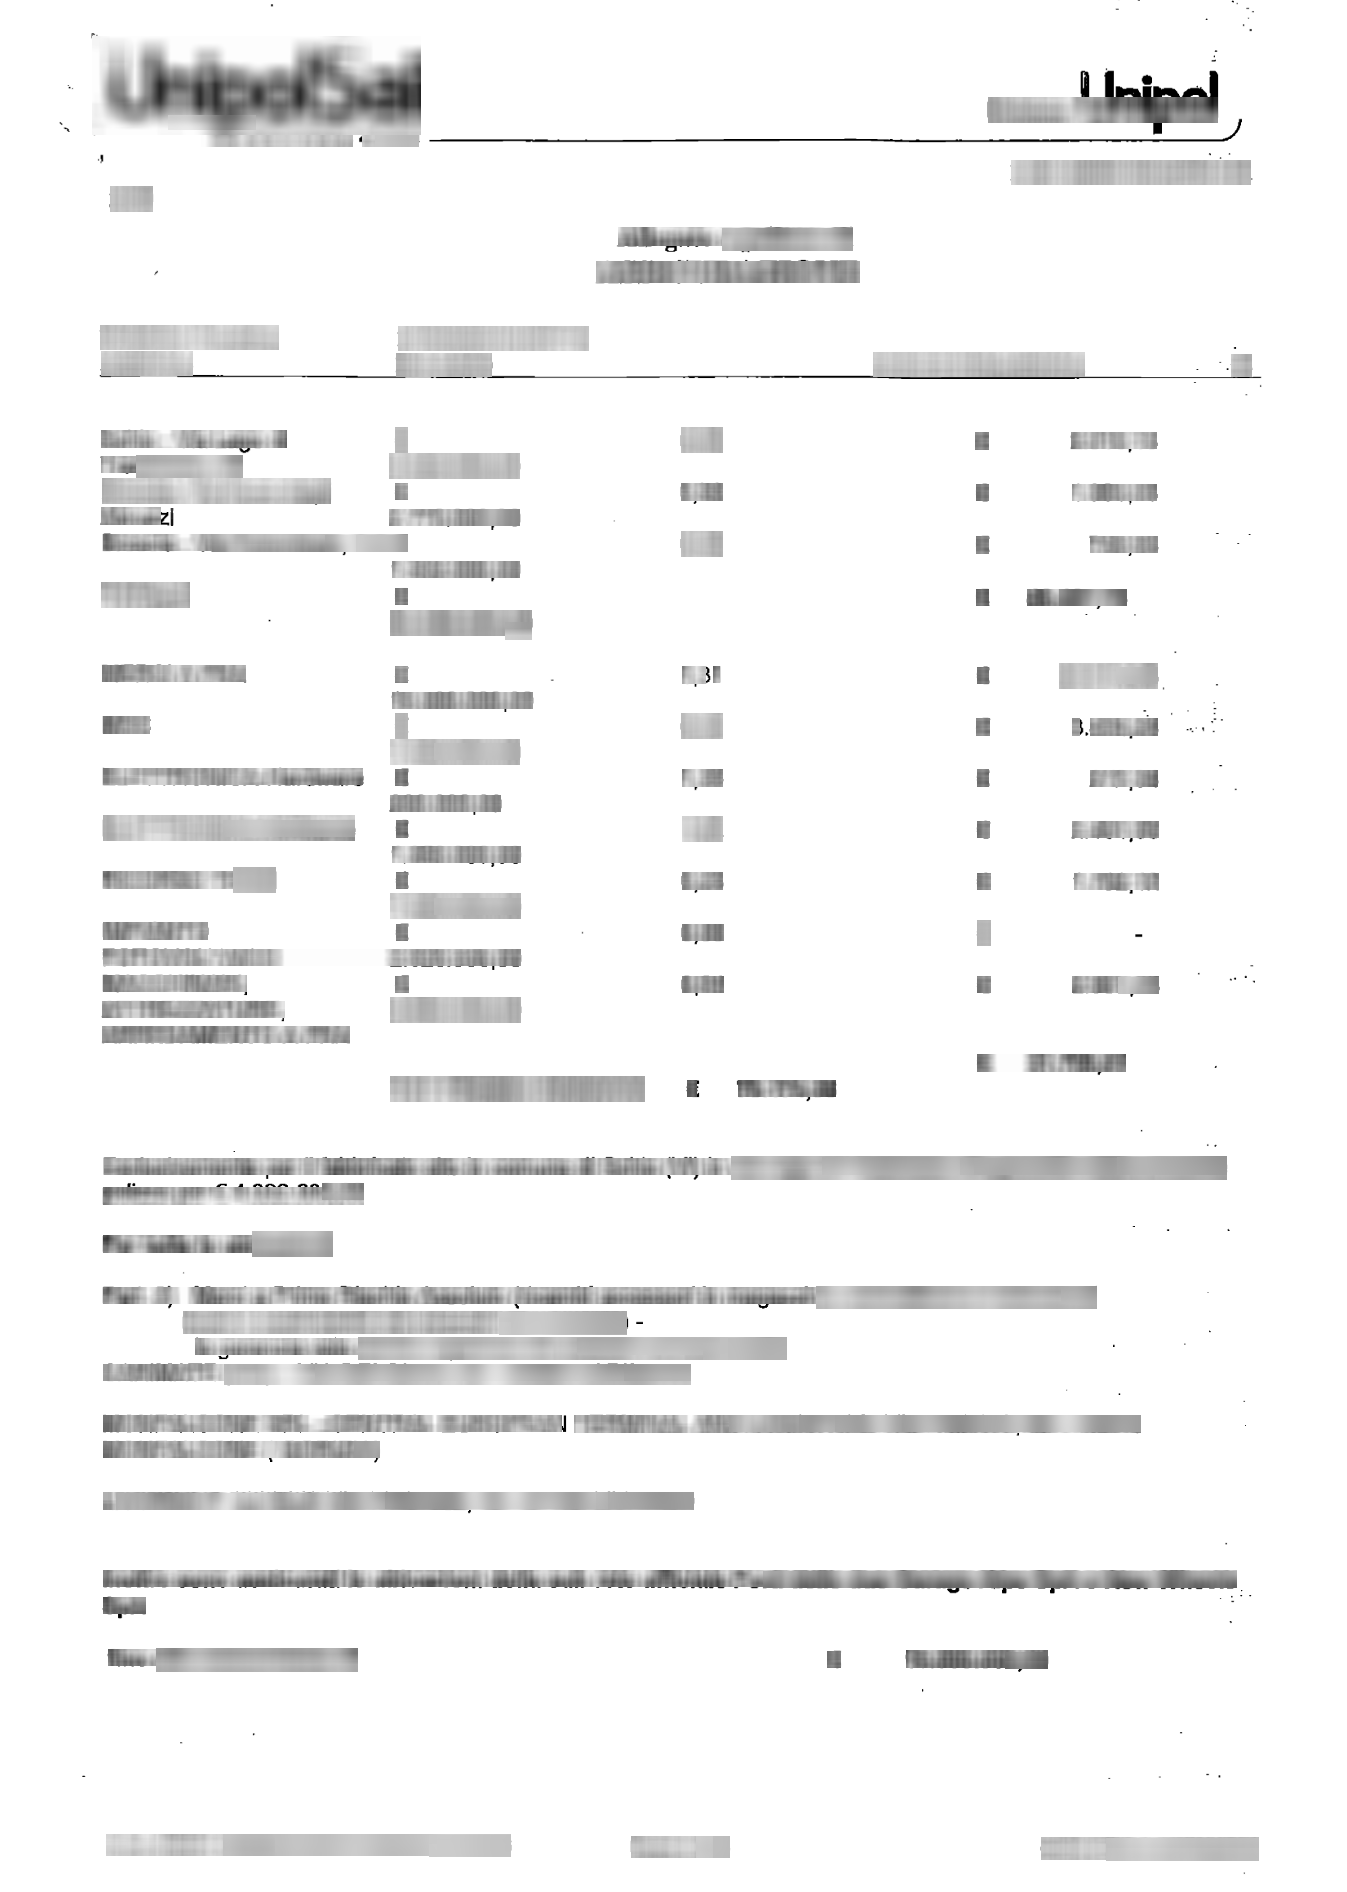
\includegraphics[width=1\columnwidth]{appendice/test0} 
    \caption{Test 0}
    \label{img:test-1}
\end{figure} 
\newpage

%============================================================================================


\begin{figure}[H]  
    \begin{minipage}{.5\columnwidth}  
        \centering  
        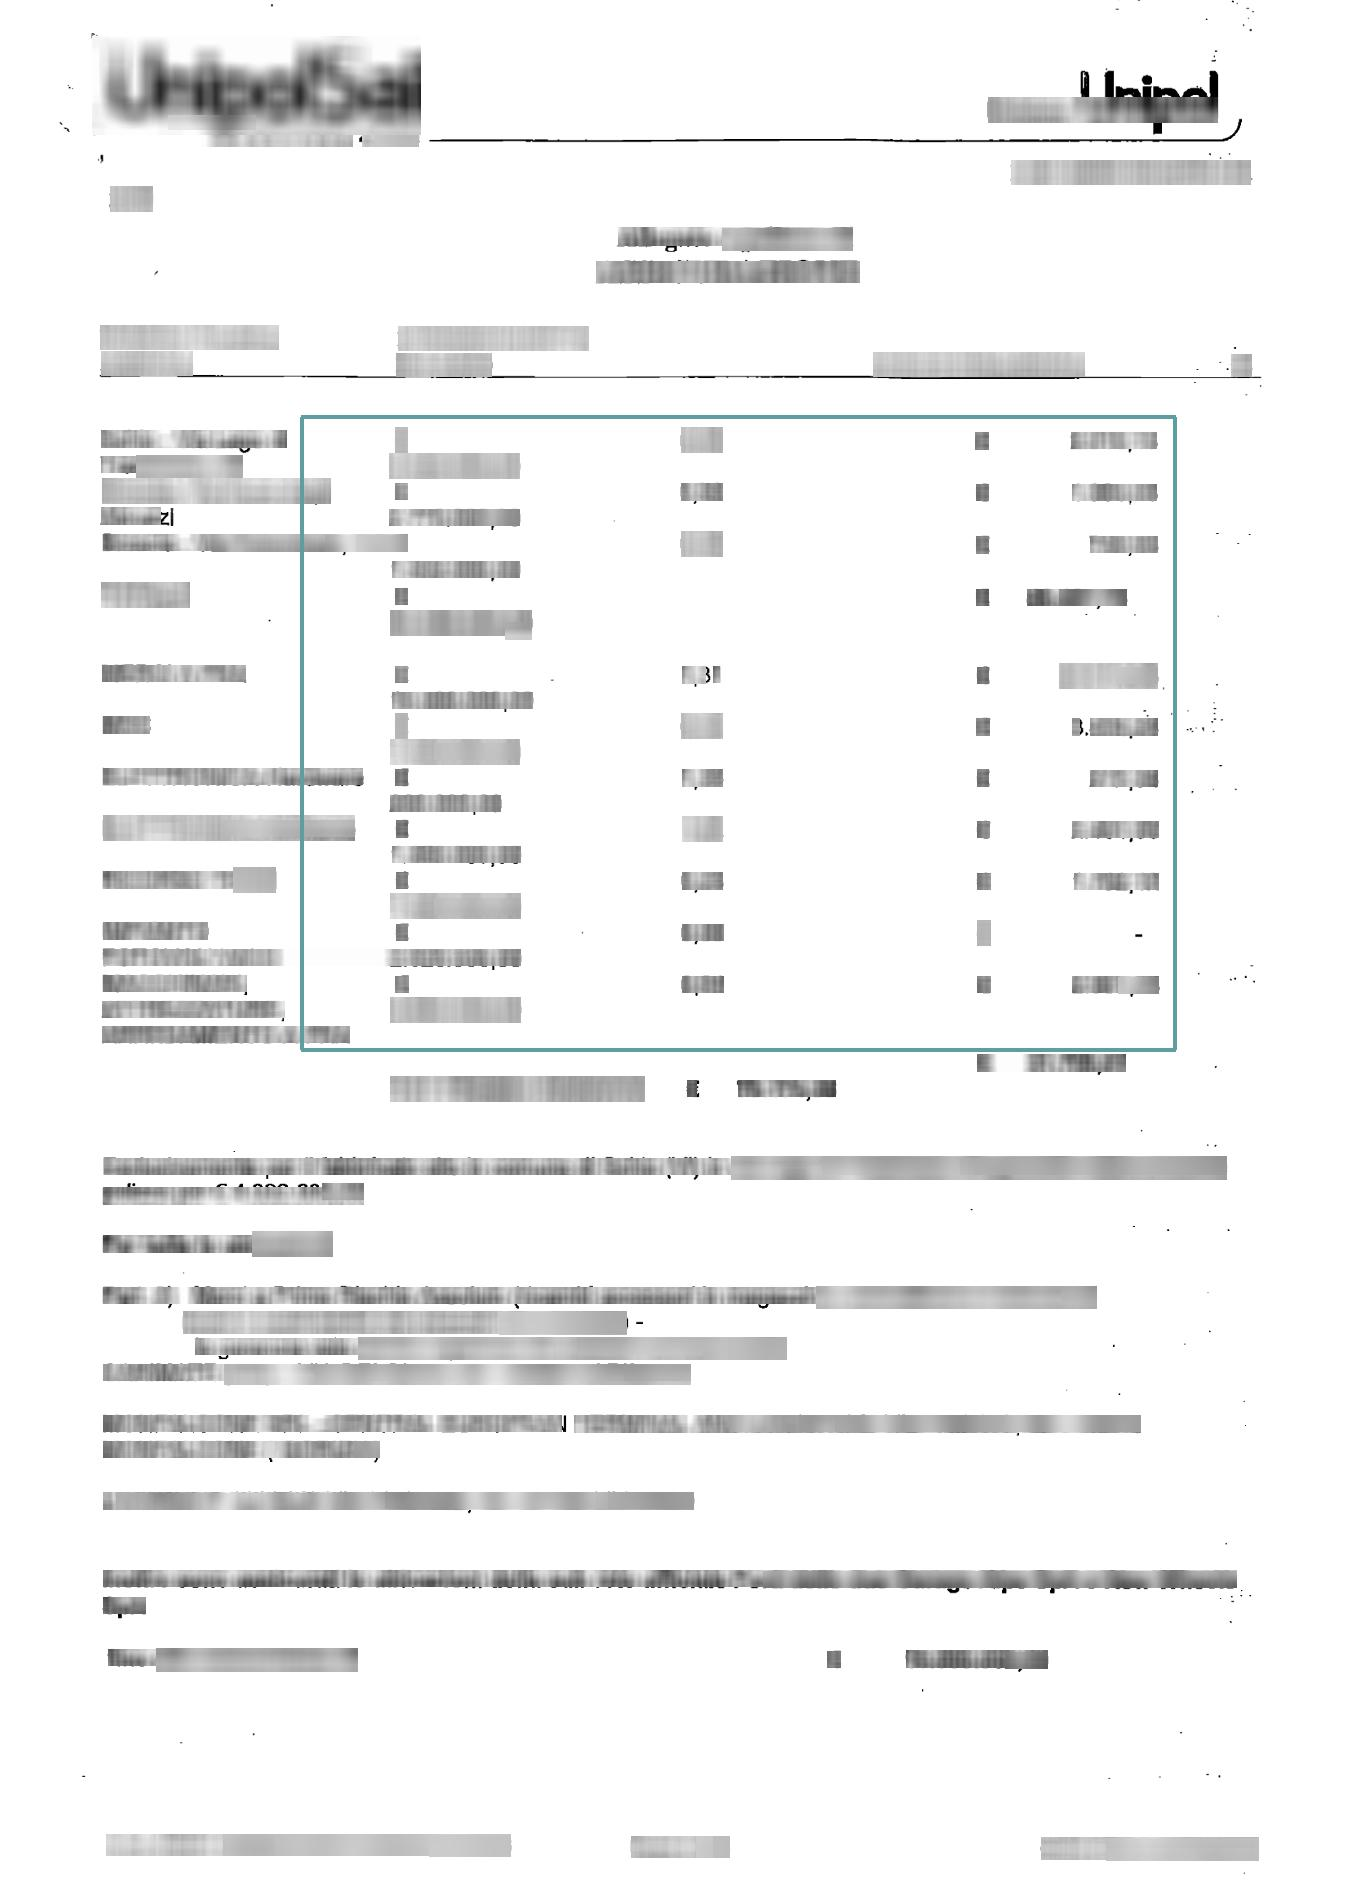
\includegraphics[width=1\columnwidth]{appendice/filtrate/test0_filtered_0_6_adam_1}  
    \end{minipage}%  
    \begin{minipage}{0.5\columnwidth}  
        \centering  
        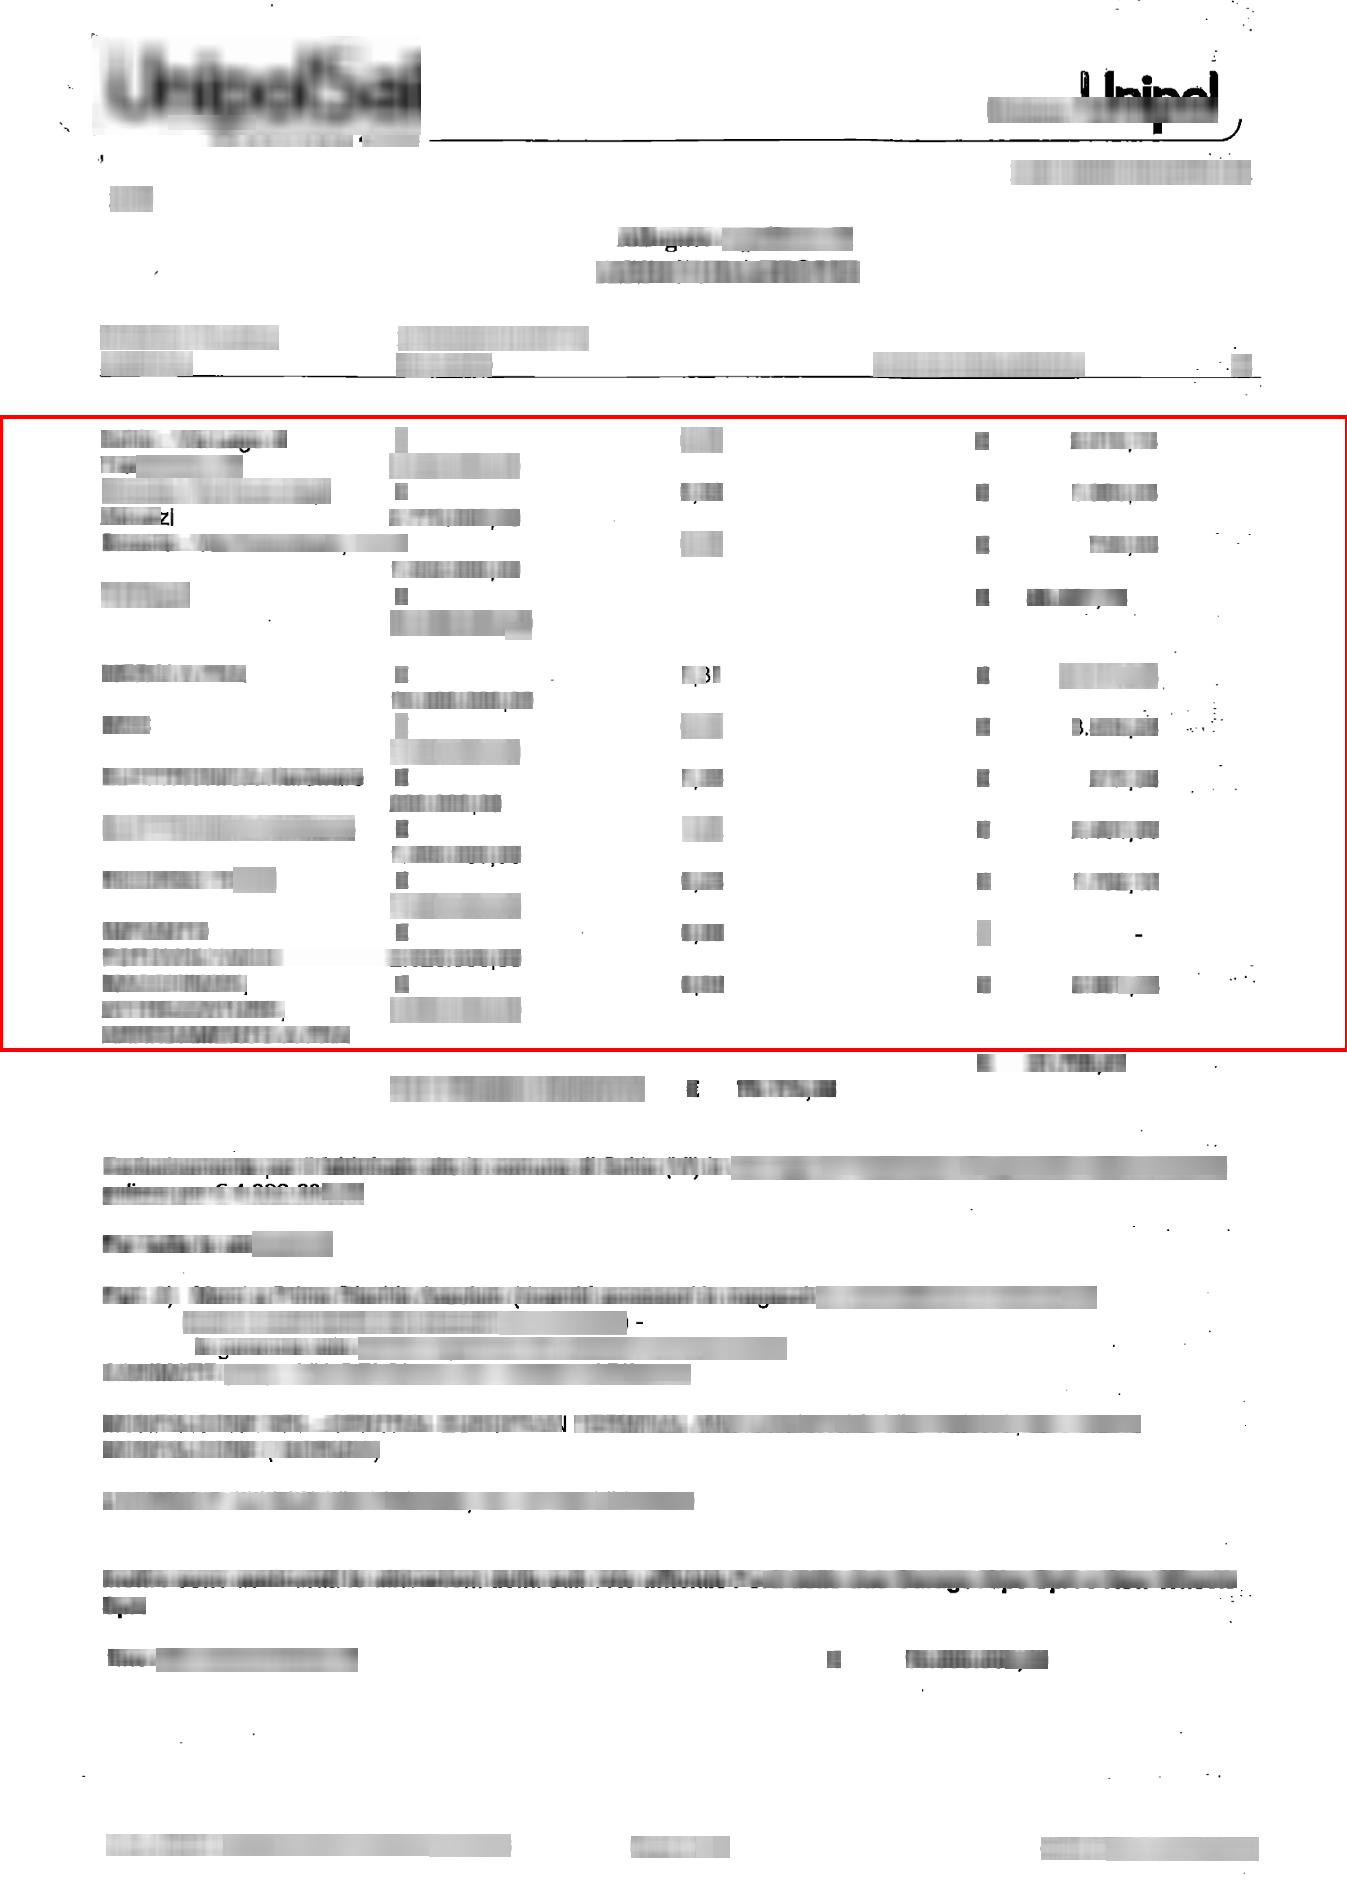
\includegraphics[width=1\columnwidth]{appendice/unite/test0_merged_0_6_adam_1}  
    \end{minipage}  
    \caption{Test 0, configurazione 1}
\end{figure}%  
Configurazione:
\begin{multicols}{2}
    \begin{lstlisting}
image_resizer {
  fixes_shape_resizer {
    width: 400
    heigth: 400
  }
}
first_stage_box_predictor {
  l2_regularizer {
    weight: 0.008
}
first_stage_nms_iou_threshold: 0.7
second_stage_box_predictor {
  l2_regularizer {
    weight: 0.004
  }
}
second_stage_post_processing {
  iou_threshold: 0.6
}
optimizer {
  adam_optimizer: {
    learning_rate: {
      manual_step_learning_rate {
        initial_learning_rate: .00008
        schedule {
          step: 4500
          learning_rate: .00004
        }
        schedule {
          step: 7000
          learning_rate: .00002
        }
        schedule {
          step: 10000
          learning_rate: .000008
        }
    ...
    }
    momentum_optimizer_value: 0.9
  }
  use_moving_average: false
}
\end{lstlisting}
\end{multicols}

%============================================================================================
\newpage
\begin{figure}[H]  
    \begin{minipage}{.5\columnwidth}  
        \centering  
        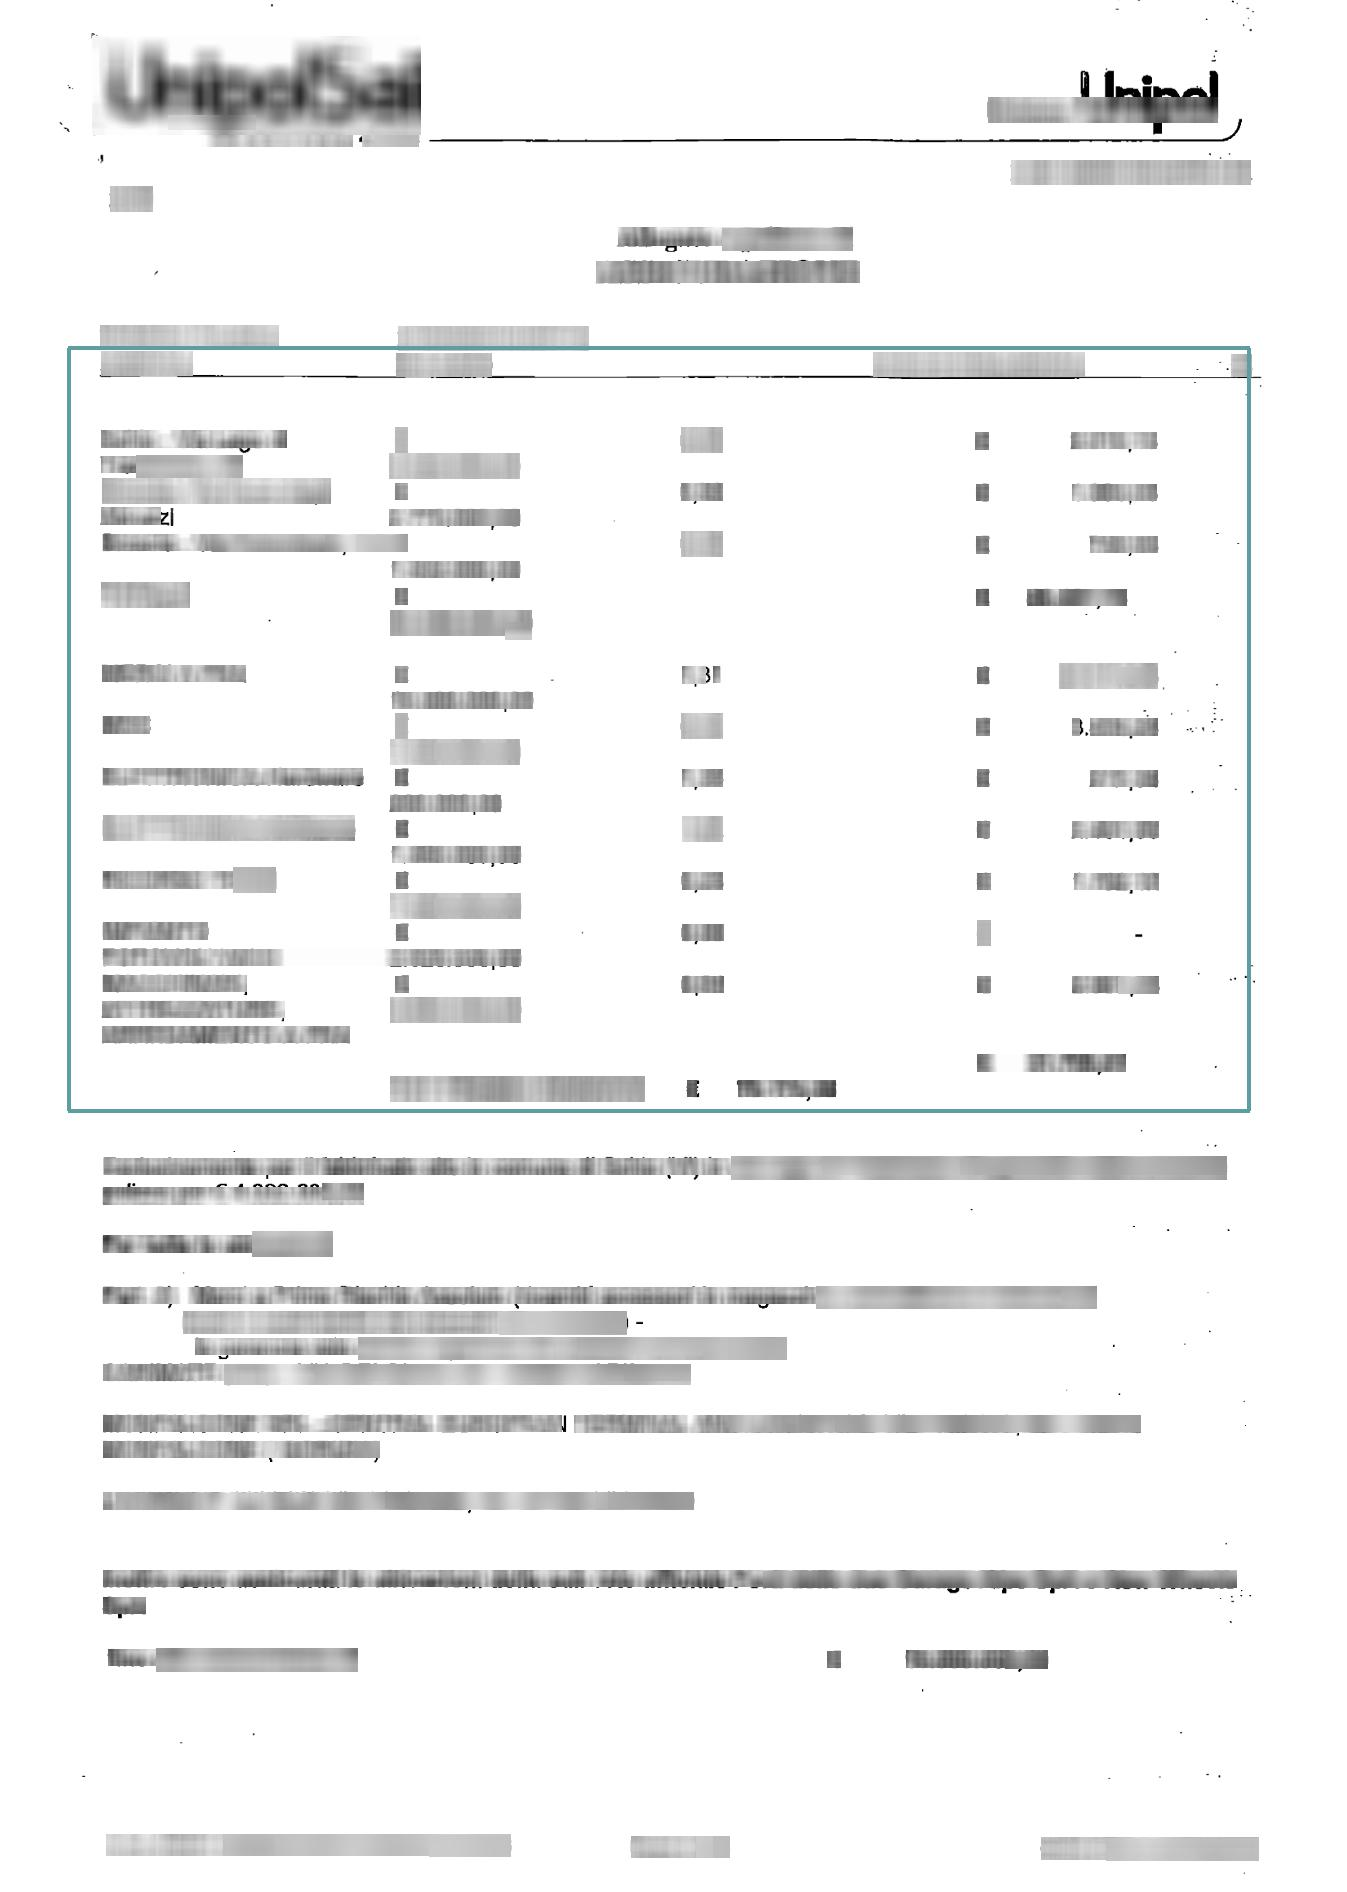
\includegraphics[width=1\columnwidth]{appendice/filtrate/test0_filtered_0_6_adam_3}  
    \end{minipage}%  
    \begin{minipage}{0.5\columnwidth}  
        \centering  
        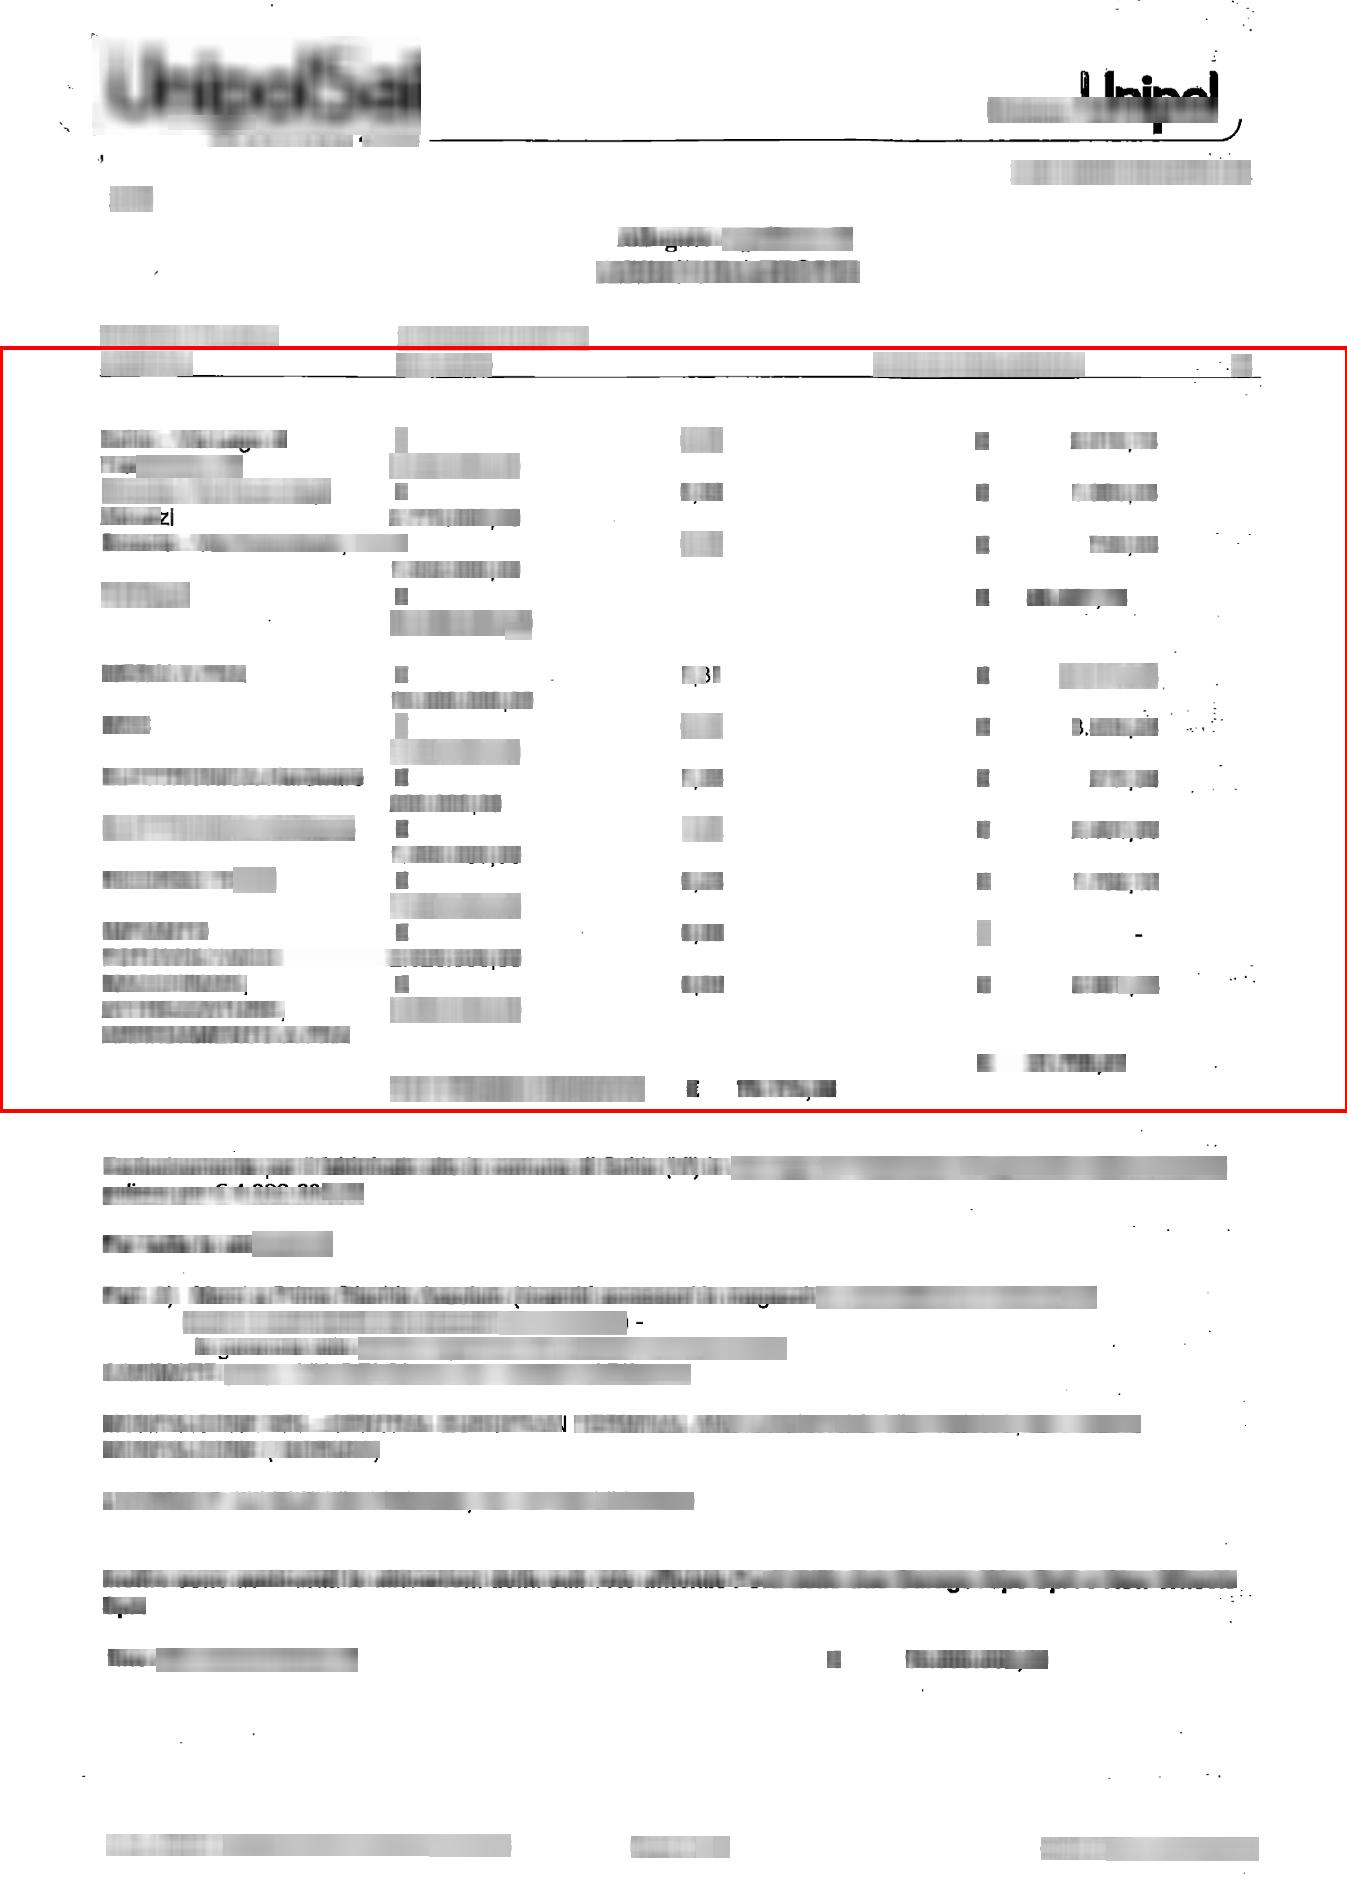
\includegraphics[width=1\columnwidth]{appendice/unite/test0_merged_0_6_adam_3}  
    \end{minipage}  
    \caption{Test 0, configurazione 2}
\end{figure}%  
Configurazione:
\begin{multicols}{2}
    \begin{lstlisting}
image_resizer {
  fixes_shape_resizer {
    width: 400
    heigth: 400
  }
}
first_stage_box_predictor {
  l2_regularizer {
    weight: 0.00001
}
first_stage_nms_iou_threshold: 0.7
second_stage_box_predictor {
  l2_regularizer {
    weight: 0.00004
  }
}
second_stage_post_processing {
  iou_threshold: 0.6
}
optimizer {
  adam_optimizer: {
    learning_rate: {
      exponential_decay_learning_rate {
        initial_learning_rate: 0.0001
          decay_steps: 600
          decay_factor: 0.95
        }
      }
    ...
  use_moving_average: false
}
    \end{lstlisting}
\end{multicols}

%============================================================================================
\newpage
\begin{figure}[H]  
    \begin{minipage}{.5\columnwidth}  
        \centering  
        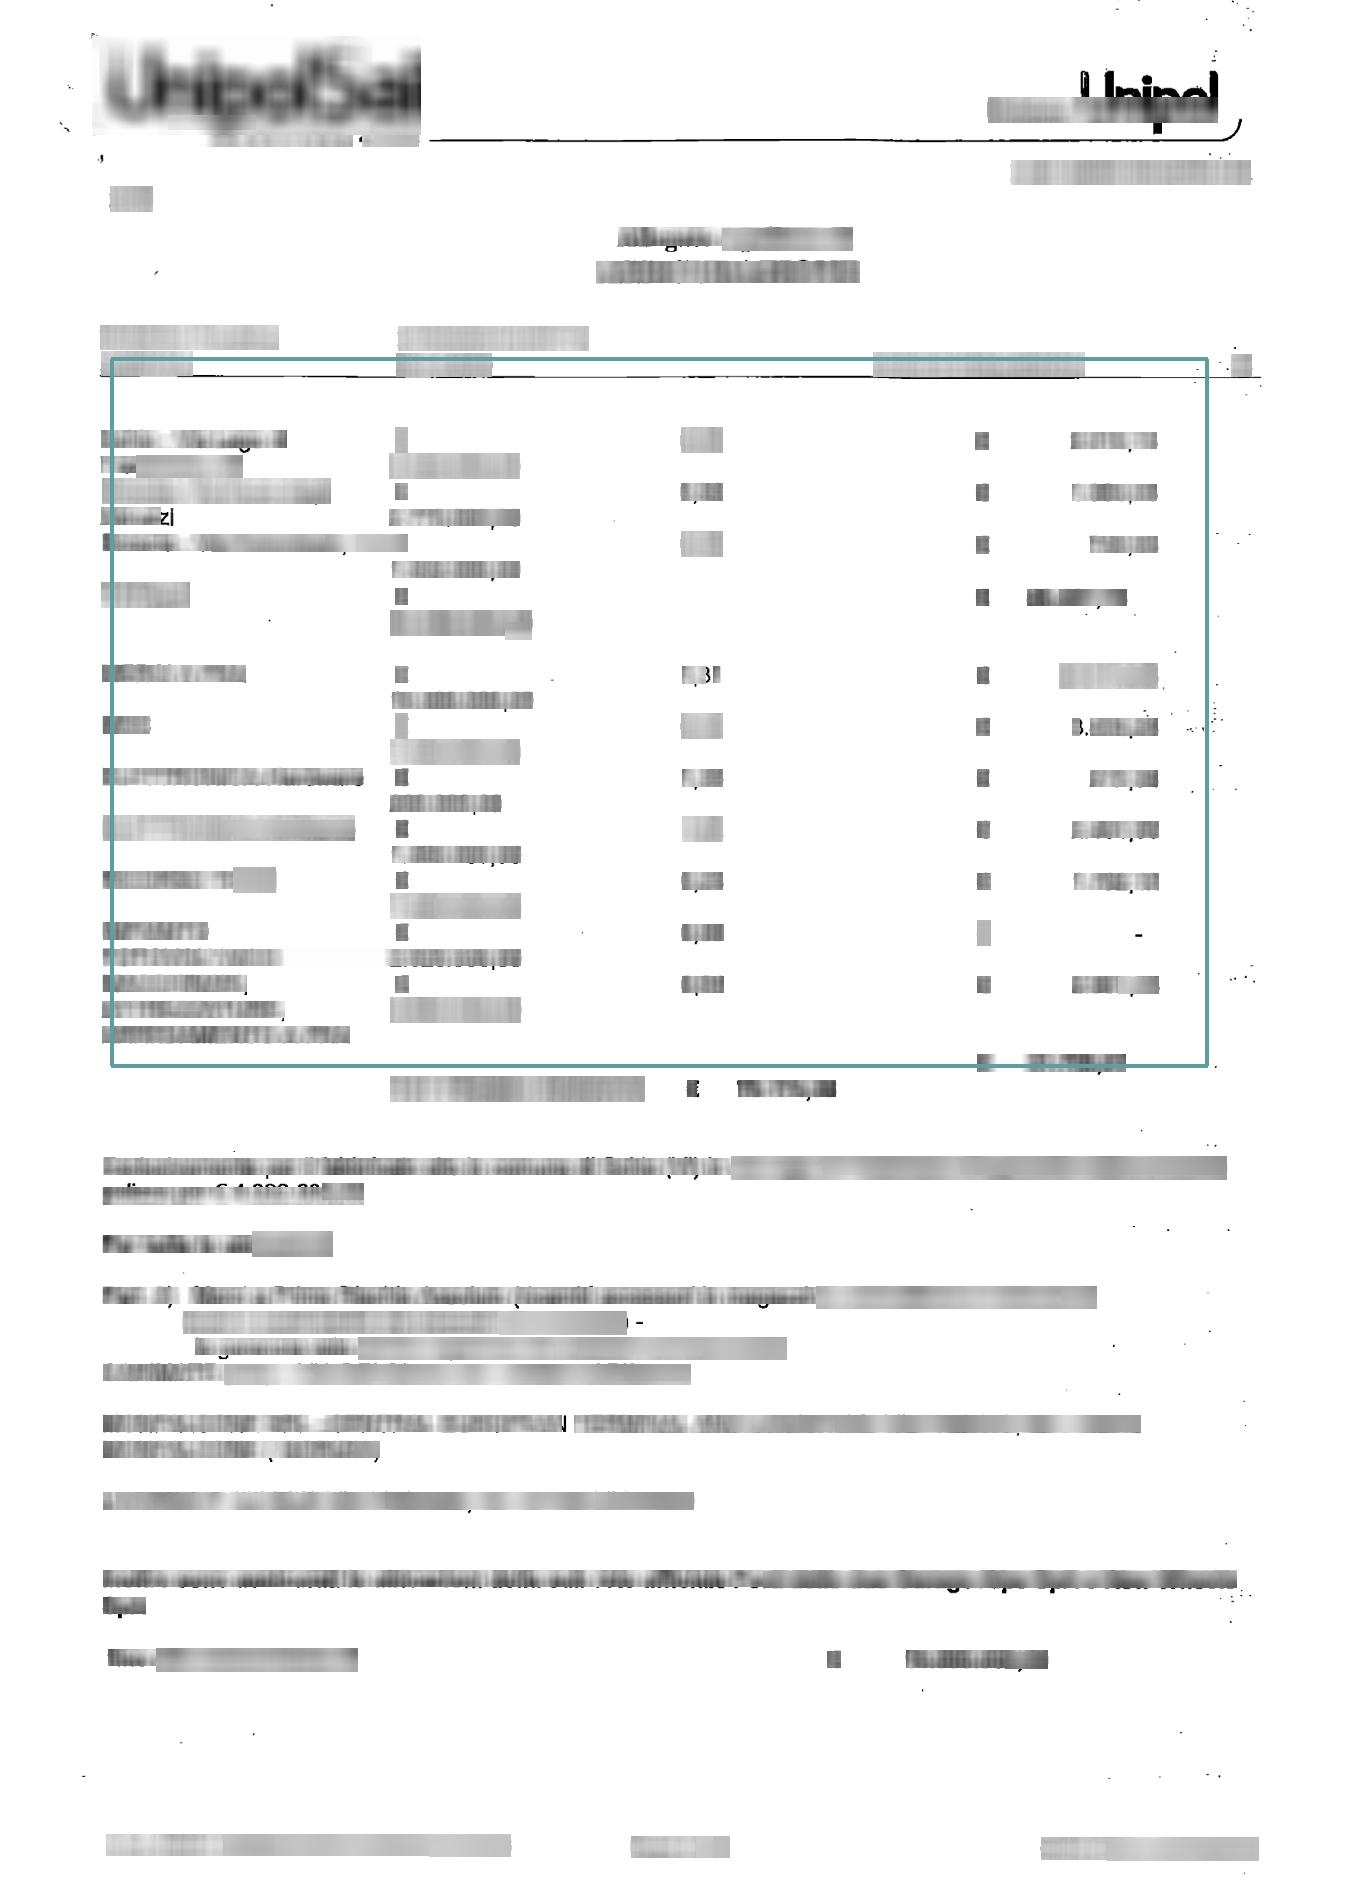
\includegraphics[width=1\columnwidth]{appendice/filtrate/test0_filtered_0_6_adam_4}  
    \end{minipage}%  
    \begin{minipage}{0.5\columnwidth}  
        \centering  
        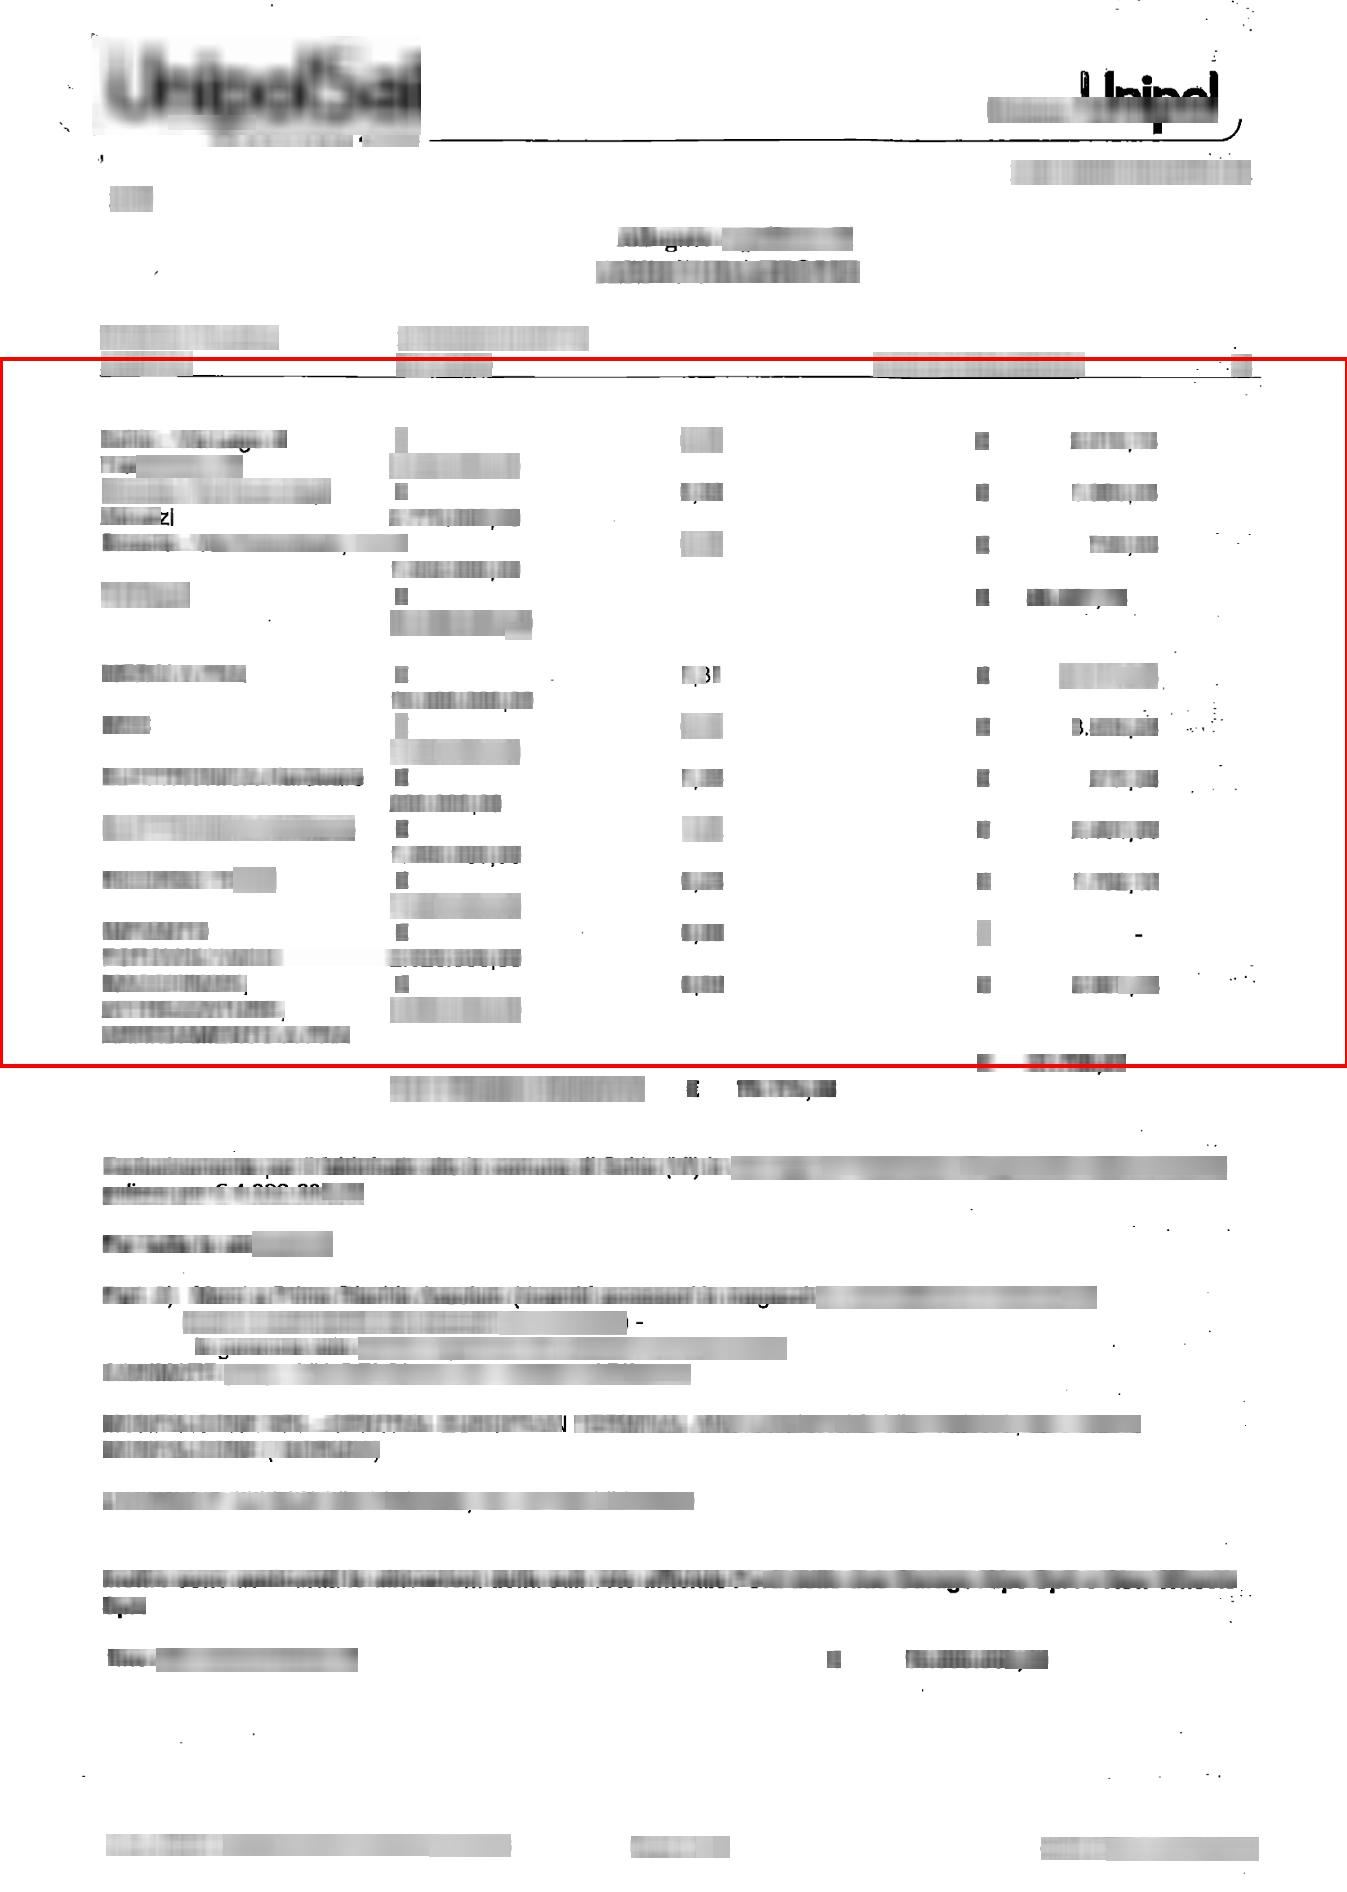
\includegraphics[width=1\columnwidth]{appendice/unite/test0_merged_0_6_adam_4}  
    \end{minipage}  
    \caption{Test 0, configurazione 3}
\end{figure}%  
Configurazione:
\begin{multicols}{2}
    \begin{lstlisting}
image_resizer {
  fixes_shape_resizer {
    width: 400
    heigth: 400
  }
}
first_stage_box_predictor {
  l2_regularizer {
    weight: 0.04
}
first_stage_nms_iou_threshold: 0.7
second_stage_box_predictor {
  l2_regularizer {
    weight: 0.004
  }
}
second_stage_post_processing {
  iou_threshold: 0.6
}
optimizer {
  adam_optimizer: {
    learning_rate: {
      exponential_decay_learning_rate {
        initial_learning_rate: 0.0001
          decay_steps: 450
          decay_factor: 0.9
        }
      }
    ...
  use_moving_average: false
}
    \end{lstlisting}
\end{multicols}

%============================================================================================
\newpage
\begin{figure}[H]  
    \begin{minipage}{.5\columnwidth}  
        \centering  
        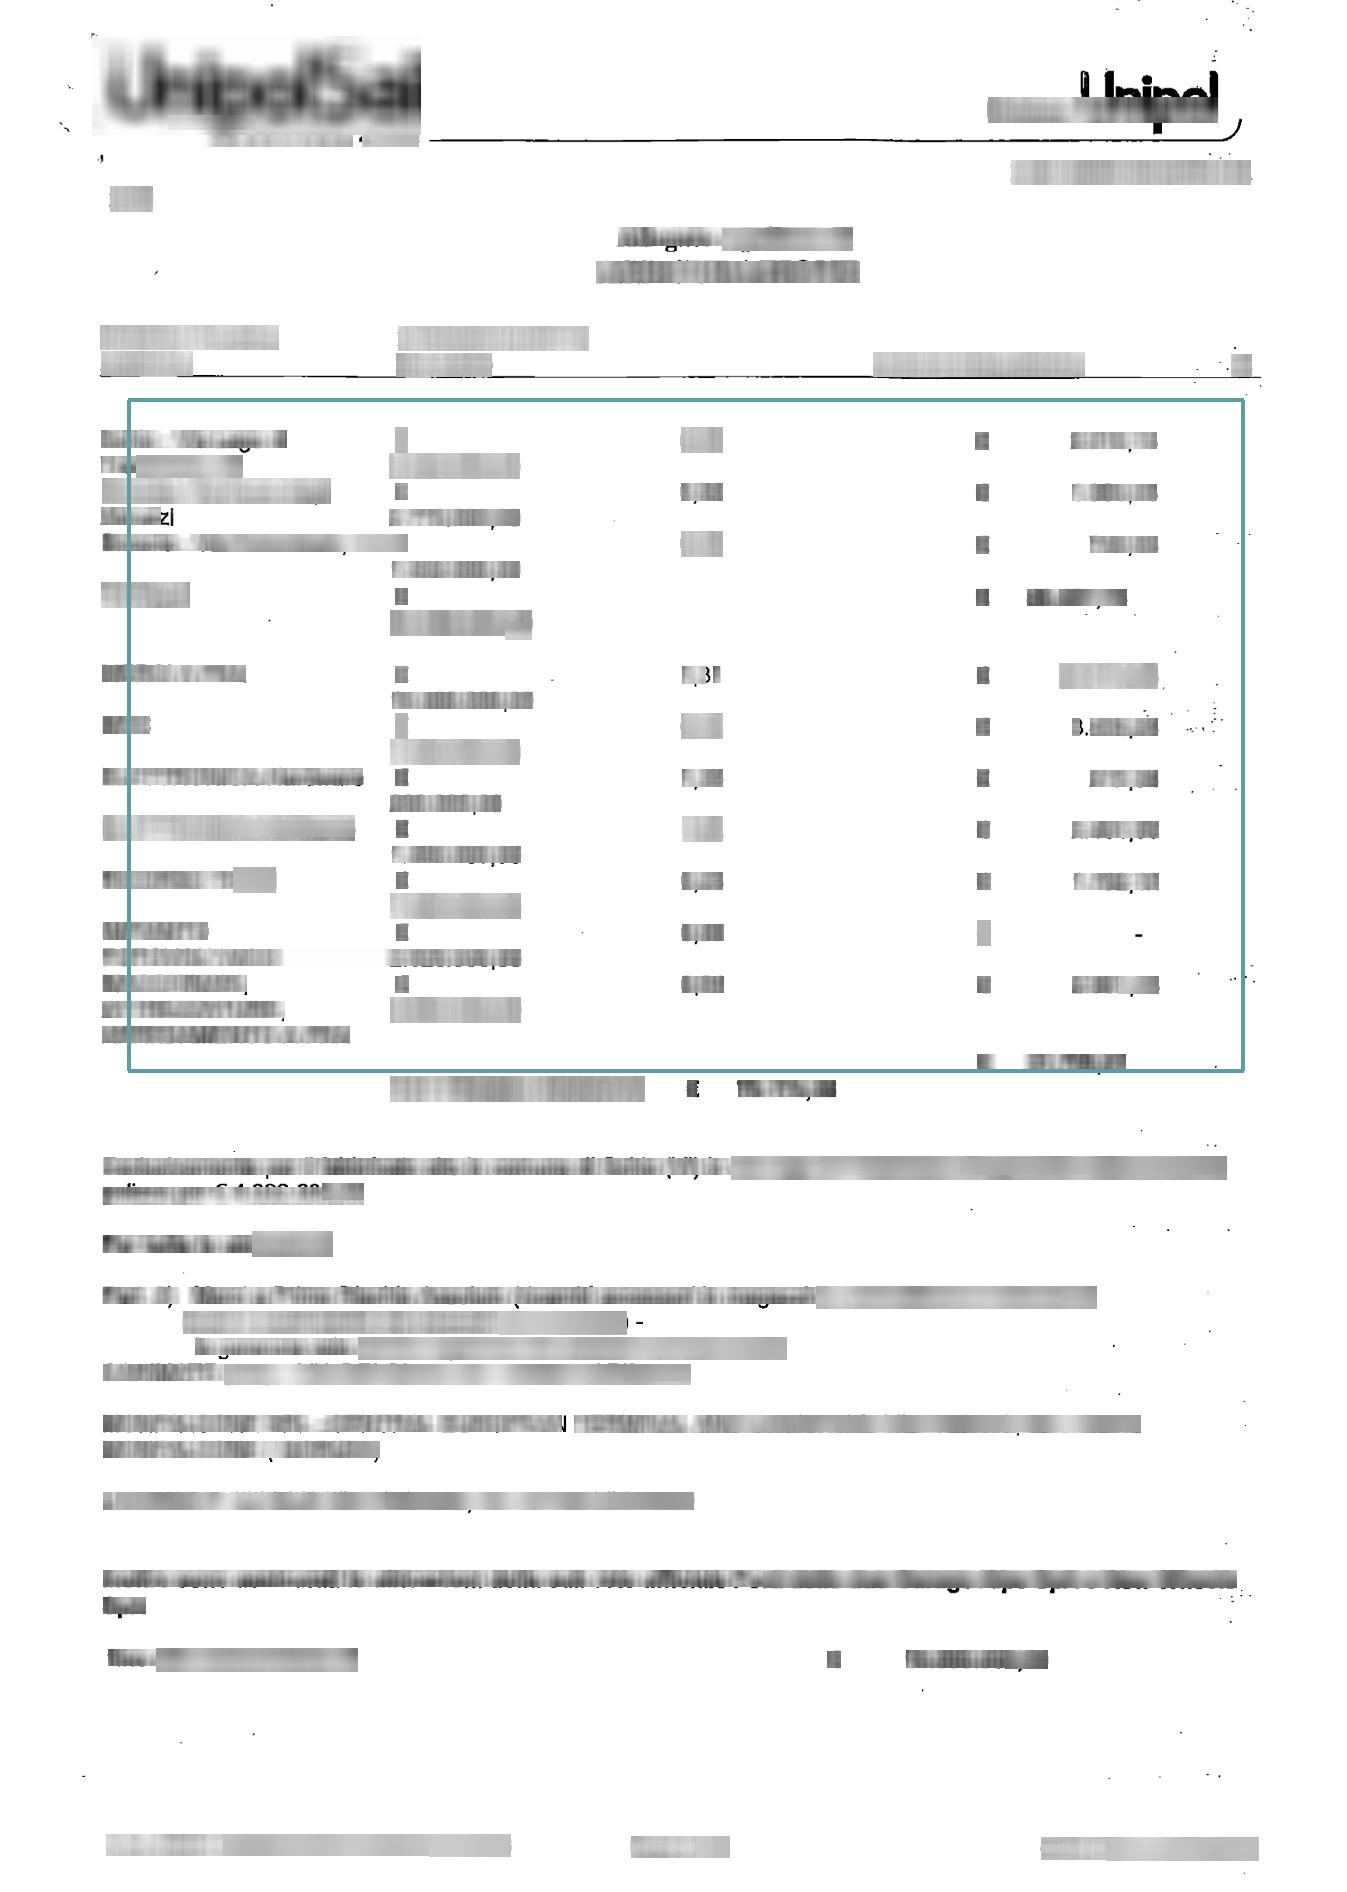
\includegraphics[width=1\columnwidth]{appendice/filtrate/test0_filtered_0_6_momentum_1}  
    \end{minipage}%  
    \begin{minipage}{0.5\columnwidth}  
        \centering  
        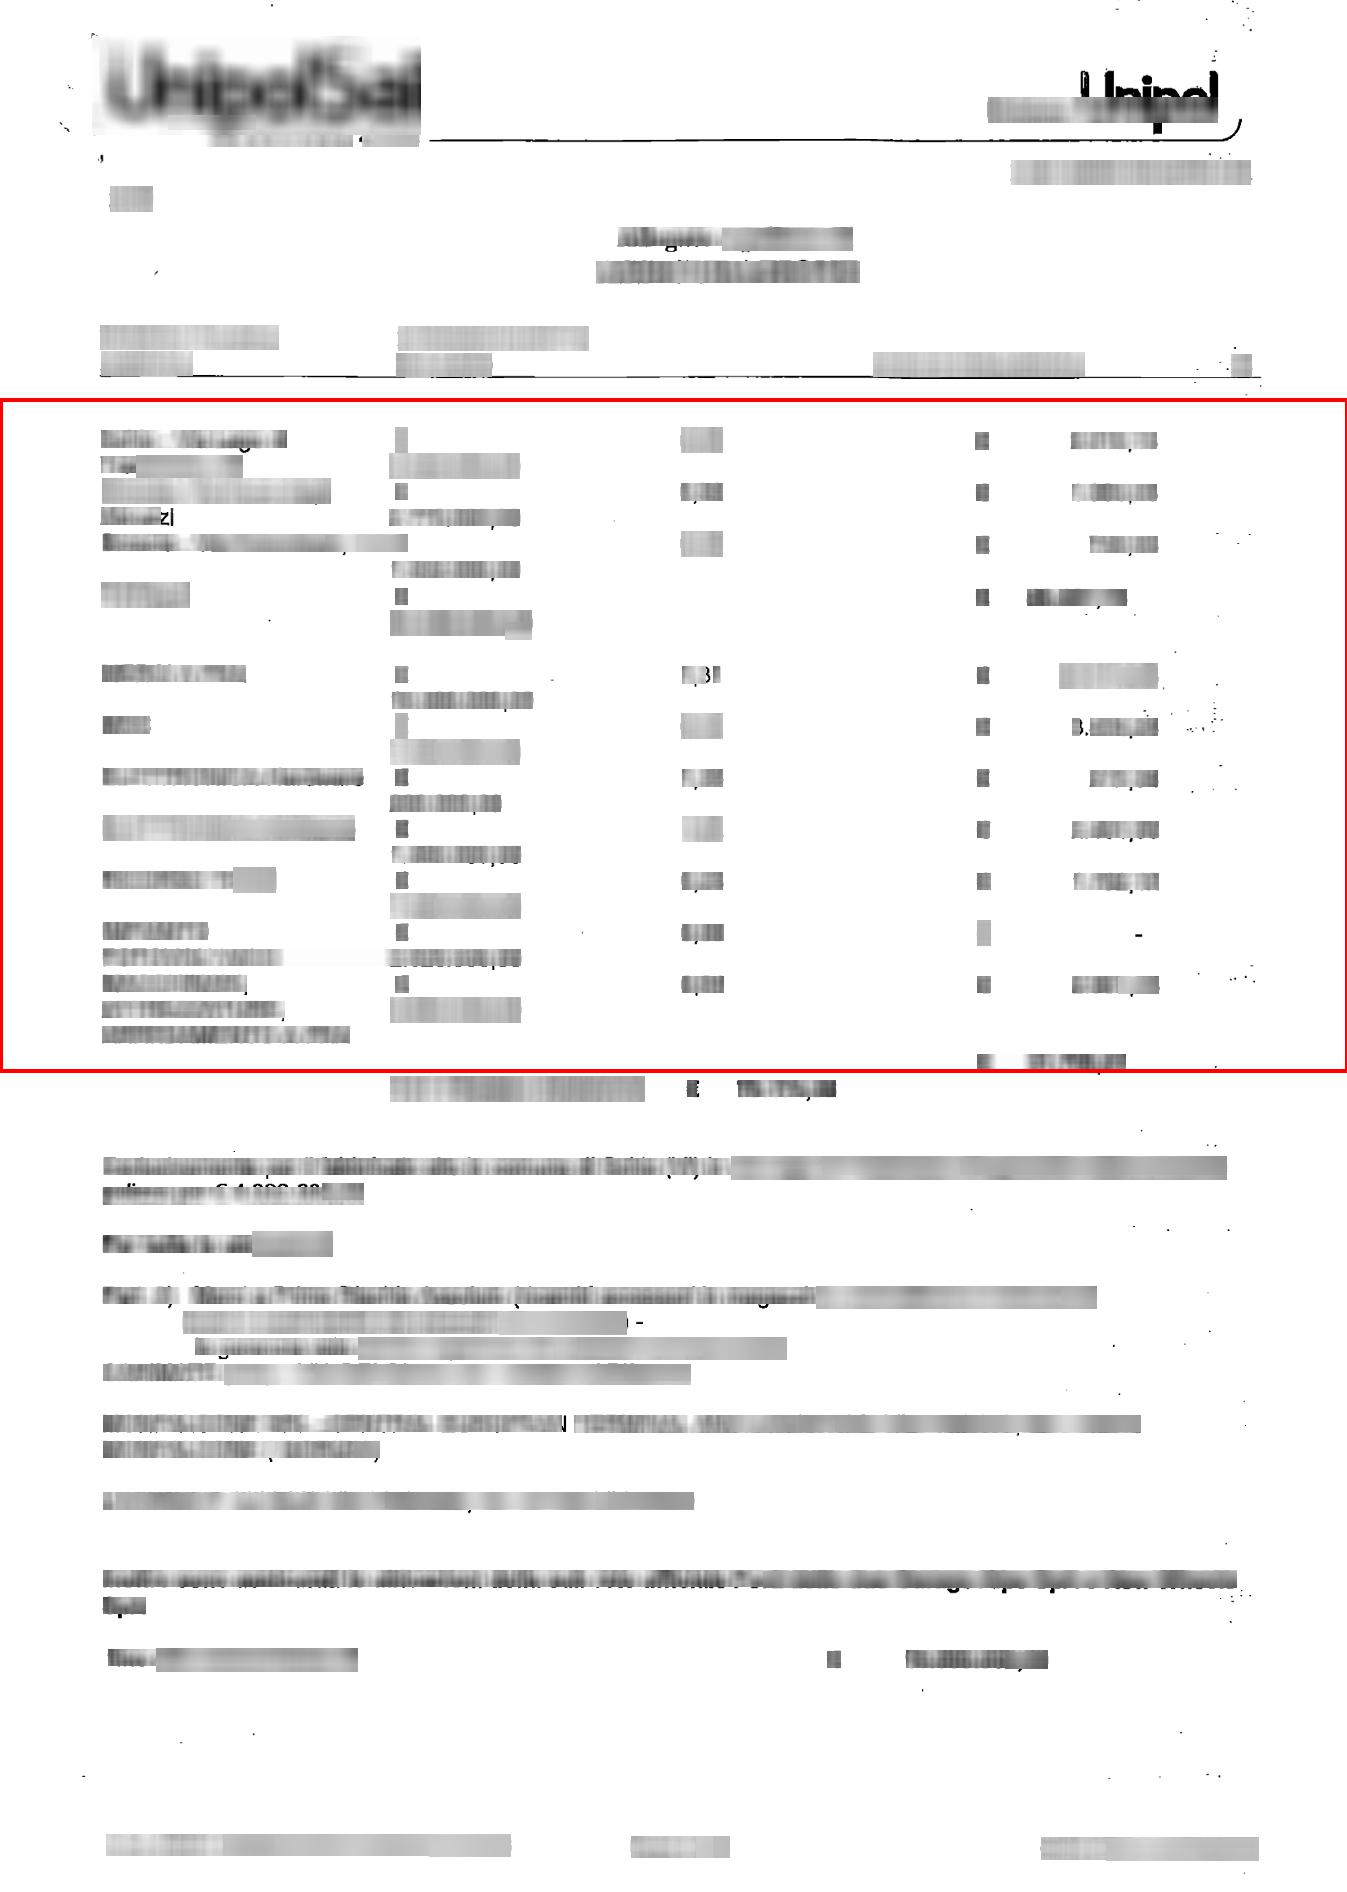
\includegraphics[width=1\columnwidth]{appendice/unite/test0_merged_0_6_momentum_1}  
    \end{minipage}  
    \caption{Test 0, configurazione 4}
\end{figure}%  
Configurazione:
\begin{multicols}{2}
    \begin{lstlisting}
image_resizer {
  fixes_shape_resizer {
    width: 400
    heigth: 400
  }
}
first_stage_box_predictor {
  l2_regularizer {
    weight: 0.00001
}
first_stage_nms_iou_threshold: 0.7
second_stage_box_predictor {
  l2_regularizer {
    weight: 0.00004
  }
}
second_stage_post_processing {
  iou_threshold: 0.6
}
optimizer {
  adam_optimizer: {
    learning_rate: {
      manual_step_learning_rate {
        initial_learning_rate: 0.0008
        schedule {
          step: 4500
          learning_rate: .0008
        }
        schedule {
          step: 7000
          learning_rate: .0004
        }
        schedule {
          step: 10000
          learning_rate: .00008
        }
    ...
    }
    momentum_optimizer_value: 0.9
  }
  use_moving_average: false
}
    \end{lstlisting}
\end{multicols}
%============================================================================================

\newpage
\begin{figure}[H]  
    \begin{minipage}{.5\columnwidth}  
        \centering  
        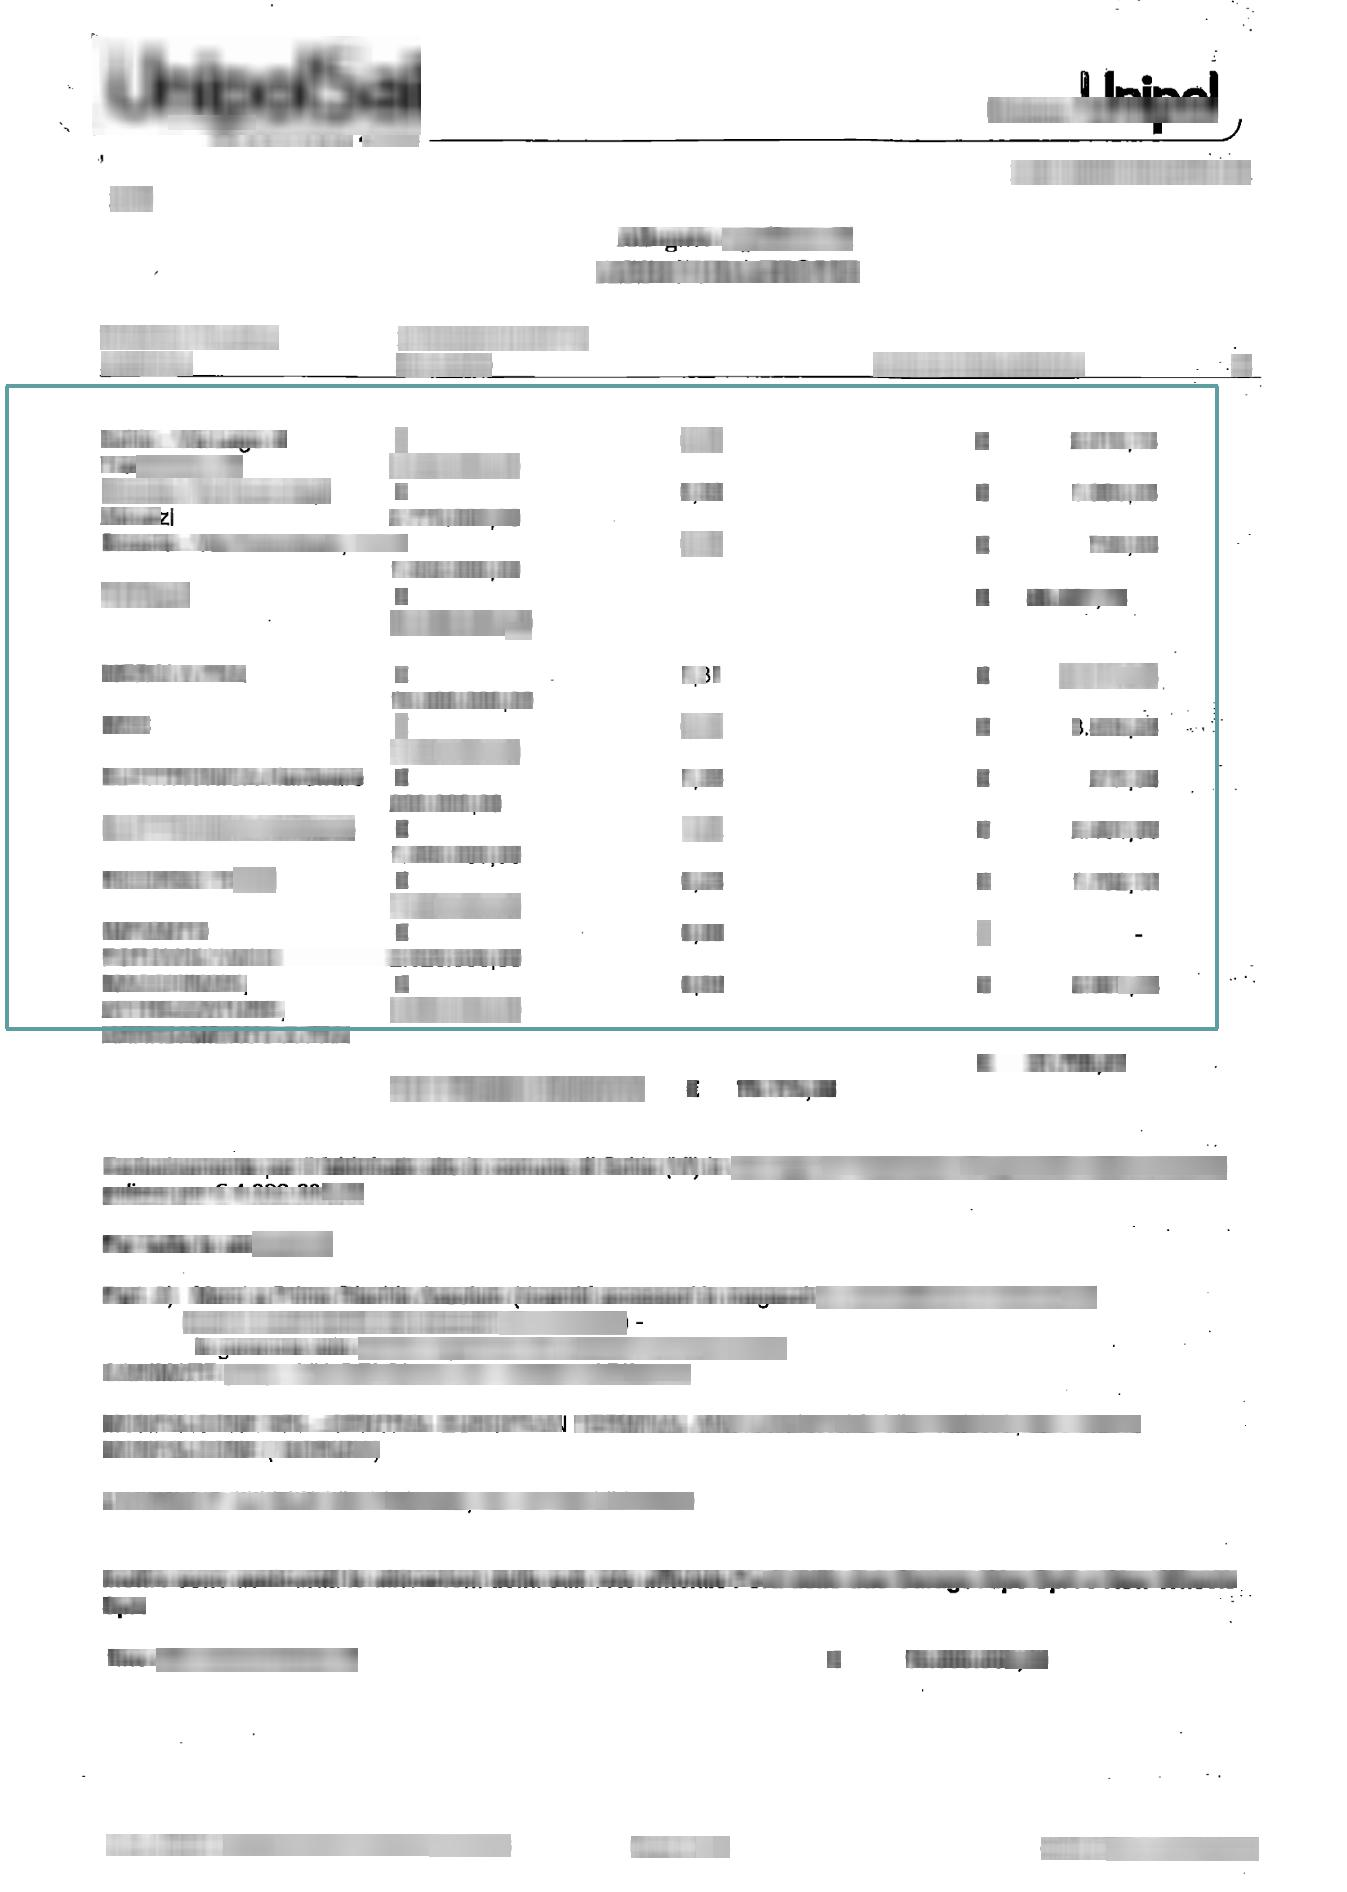
\includegraphics[width=1\columnwidth]{appendice/filtrate/test0_filtered_0_6_momentum_10k_jpg}  
    \end{minipage}%  
    \begin{minipage}{0.5\columnwidth}  
        \centering  
        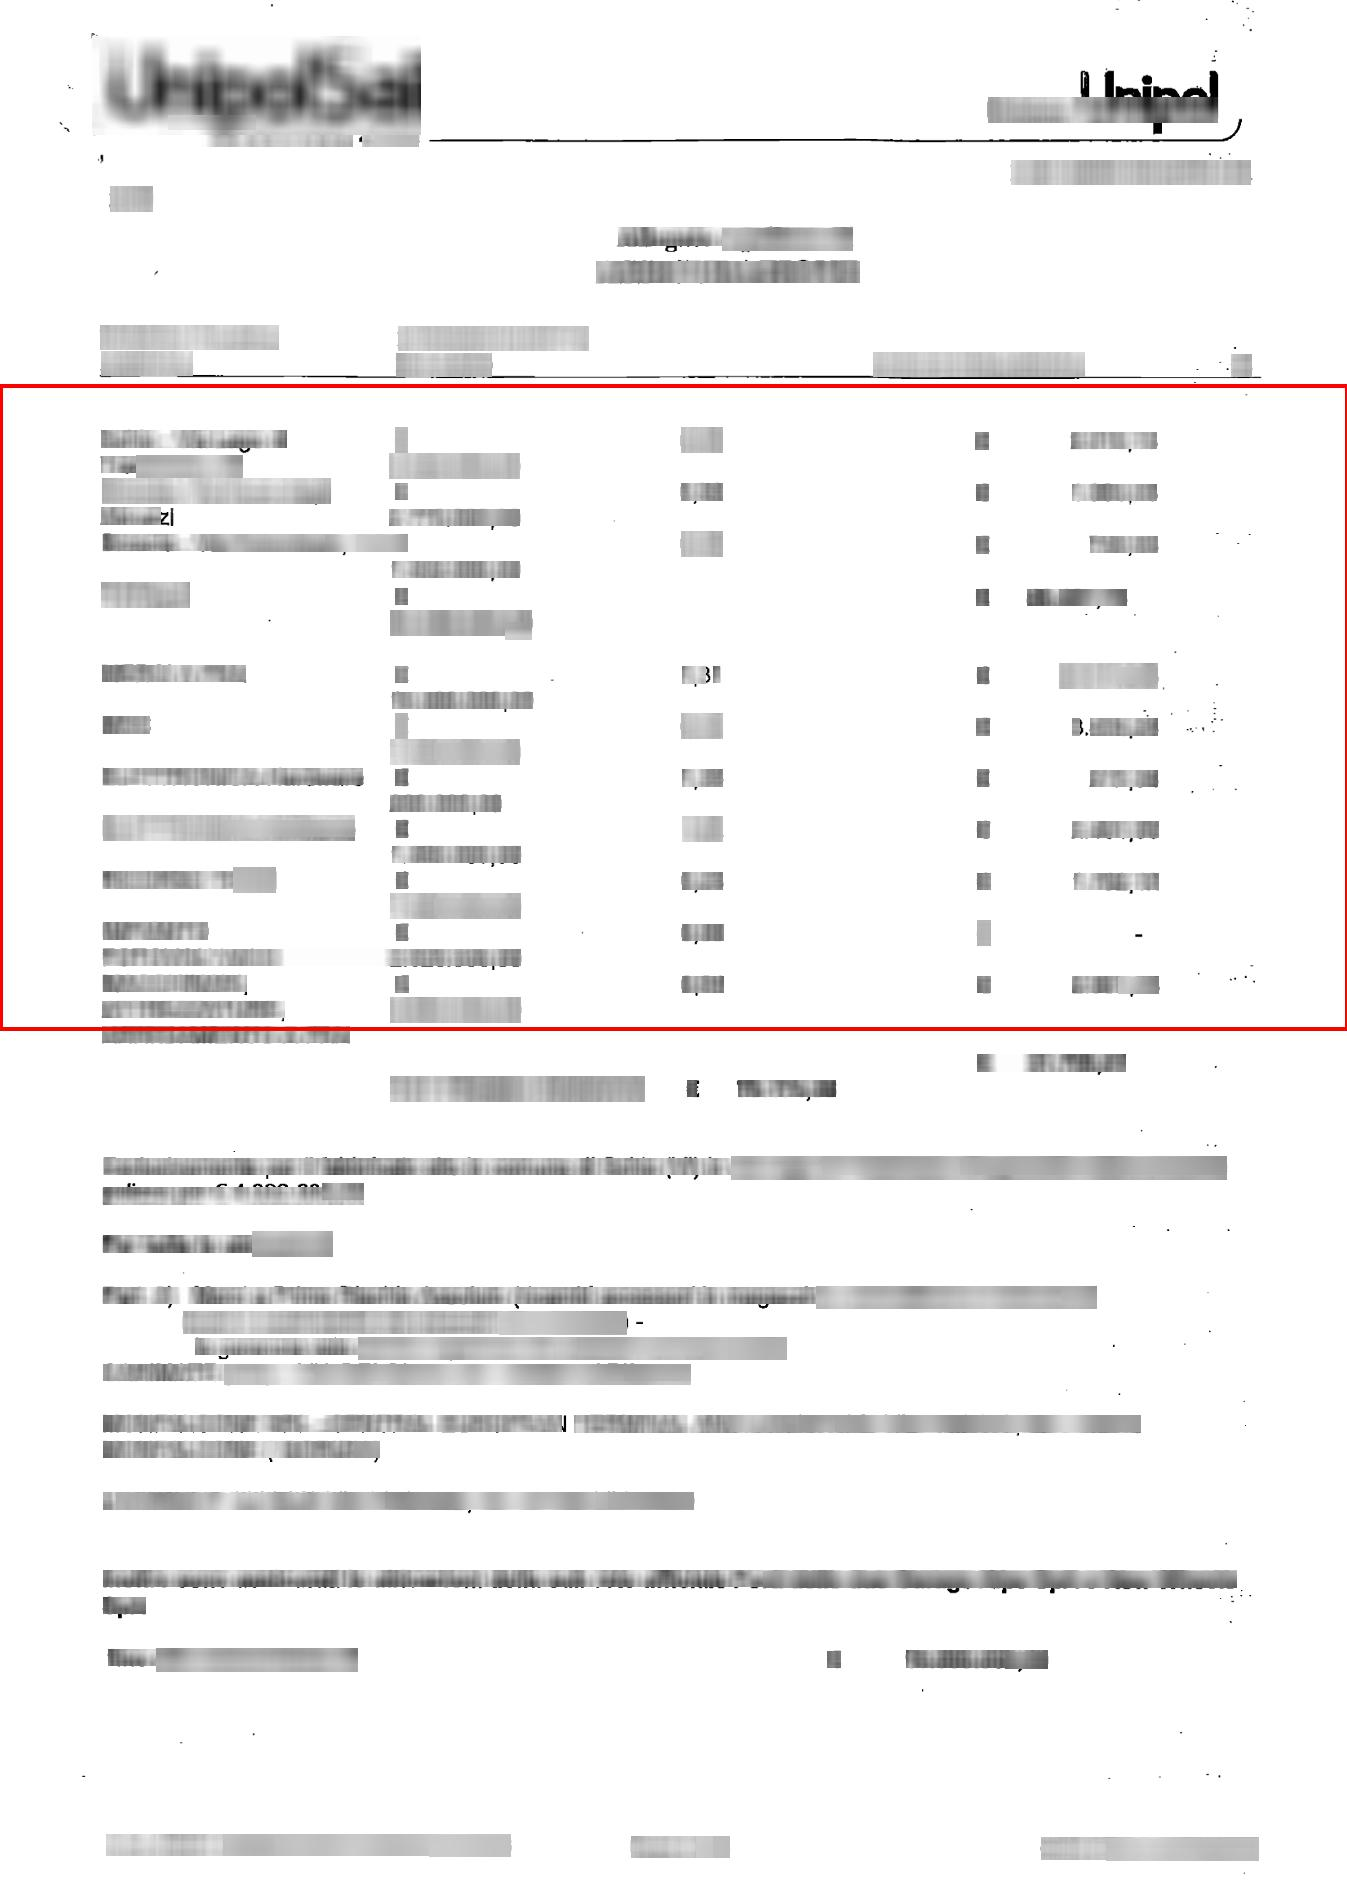
\includegraphics[width=1\columnwidth]{appendice/unite/test0_merged_0_6_momentum_10k_jpg}  
    \end{minipage}  
    \caption{Test 0, configurazione 5}
\end{figure}%  
Configurazione:
\begin{multicols}{2}
    \begin{lstlisting}
image_resizer {
  fixes_shape_resizer {
    width: 400
    heigth: 400
  }
}
first_stage_box_predictor {
  l2_regularizer {
    weight: 0.004
}
first_stage_nms_iou_threshold: 0.7
second_stage_box_predictor {
  l2_regularizer {
    weight: 0.004
  }
}
second_stage_post_processing {
  iou_threshold: 0.6
}
optimizer {
  adam_optimizer: {
    learning_rate: {
      manual_step_learning_rate {
        initial_learning_rate: 0.0004
        schedule {
          step: 4500
          learning_rate: .0002
        }
        schedule {
          step: 7000
          learning_rate: .00002
        }
        schedule {
          step: 10000
          learning_rate: .000002
        }
    ...
    }
    momentum_optimizer_value: 0.9
  }
  use_moving_average: false
}
    \end{lstlisting}
\end{multicols}
%============================================================================================

\newpage
\begin{figure}[H]  
    \begin{minipage}{.5\columnwidth}  
        \centering  
        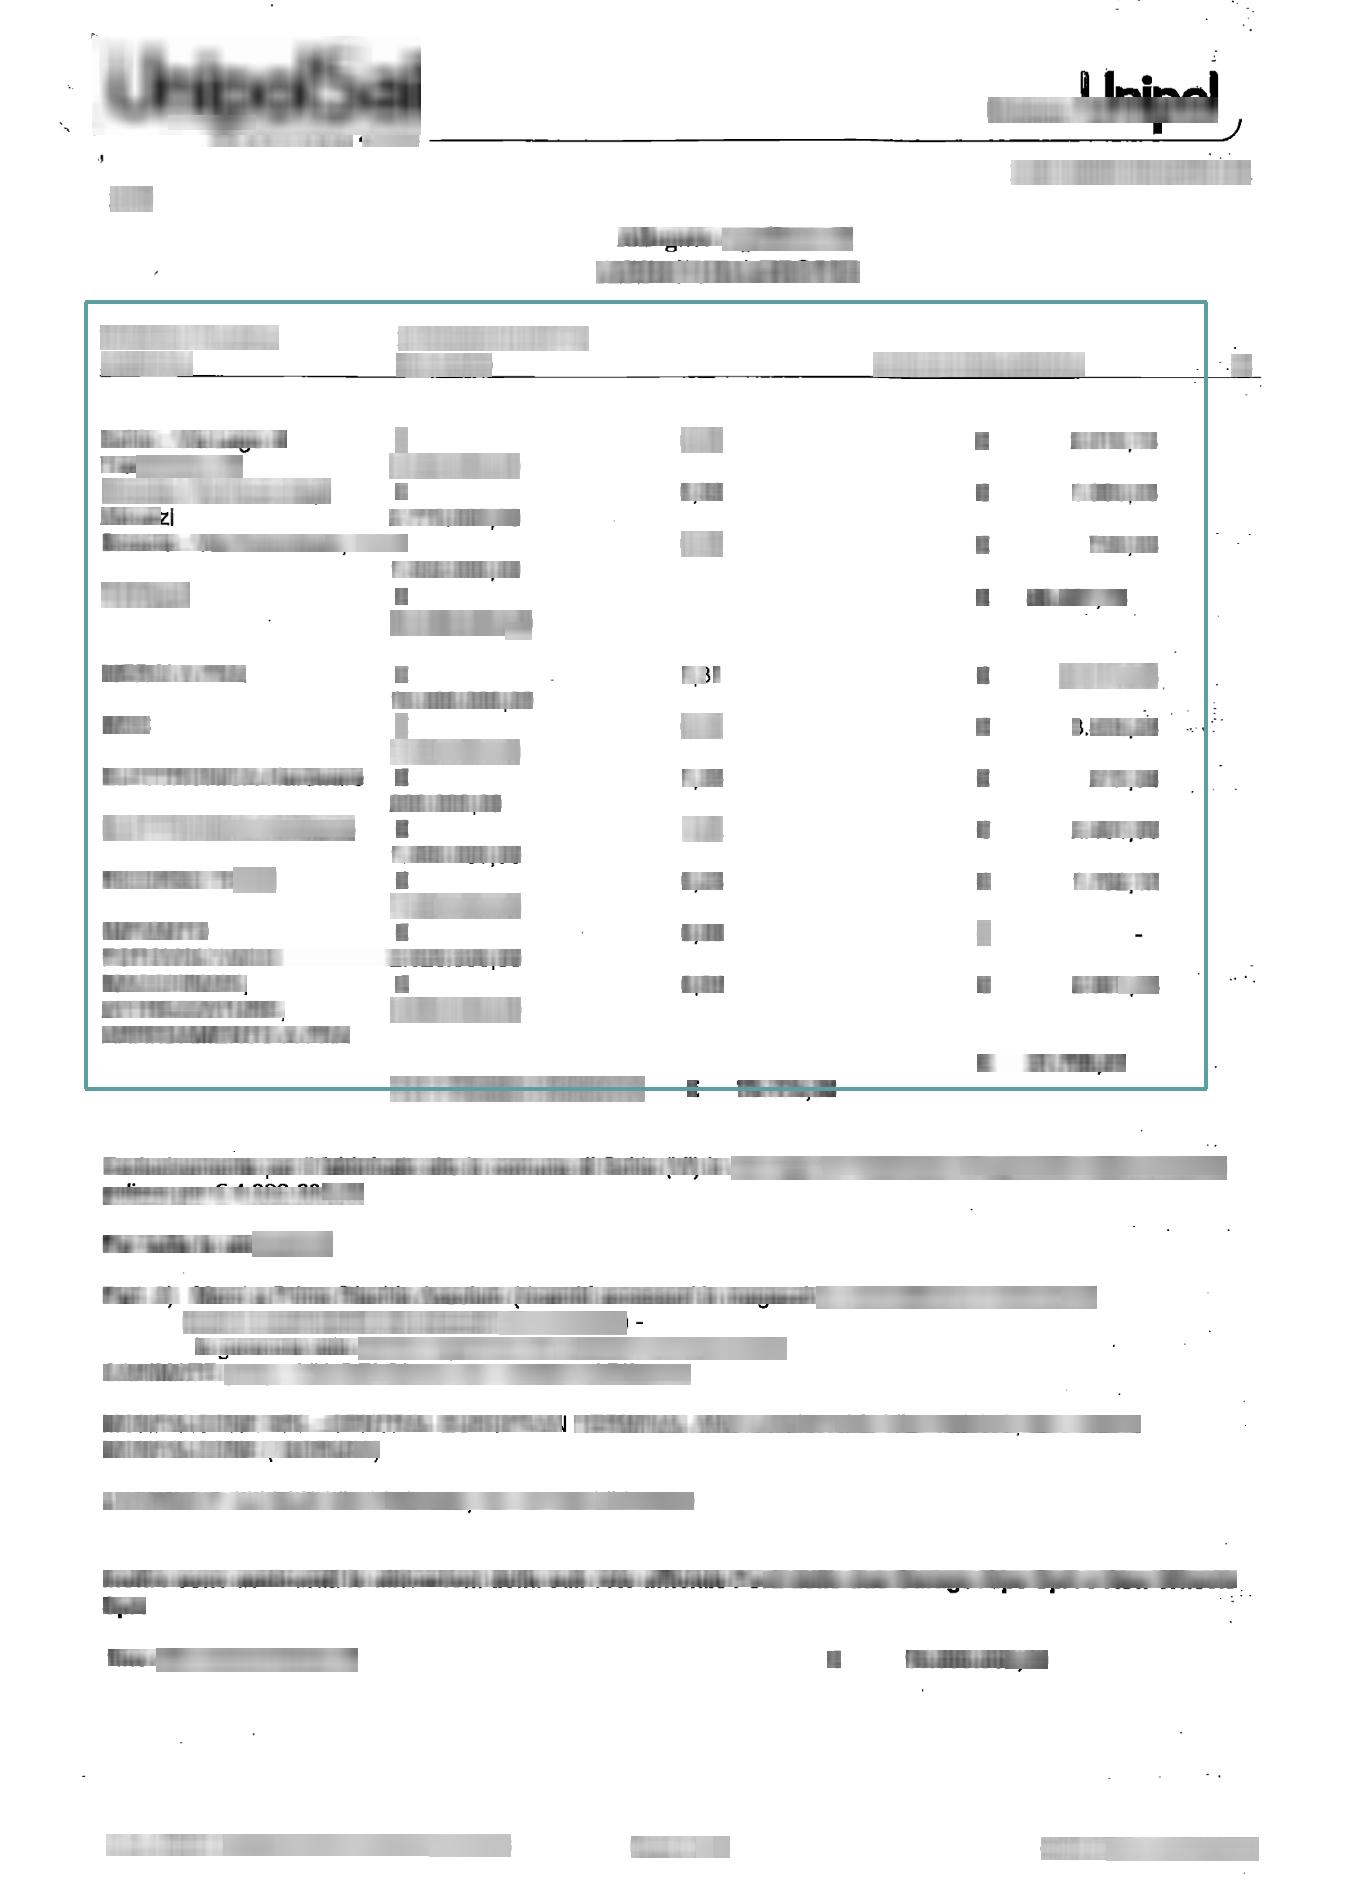
\includegraphics[width=1\columnwidth]{appendice/filtrate/test0_filtered_0_6_momentum_optimizer_1batch}  
    \end{minipage}%  
    \begin{minipage}{0.5\columnwidth}  
        \centering  
        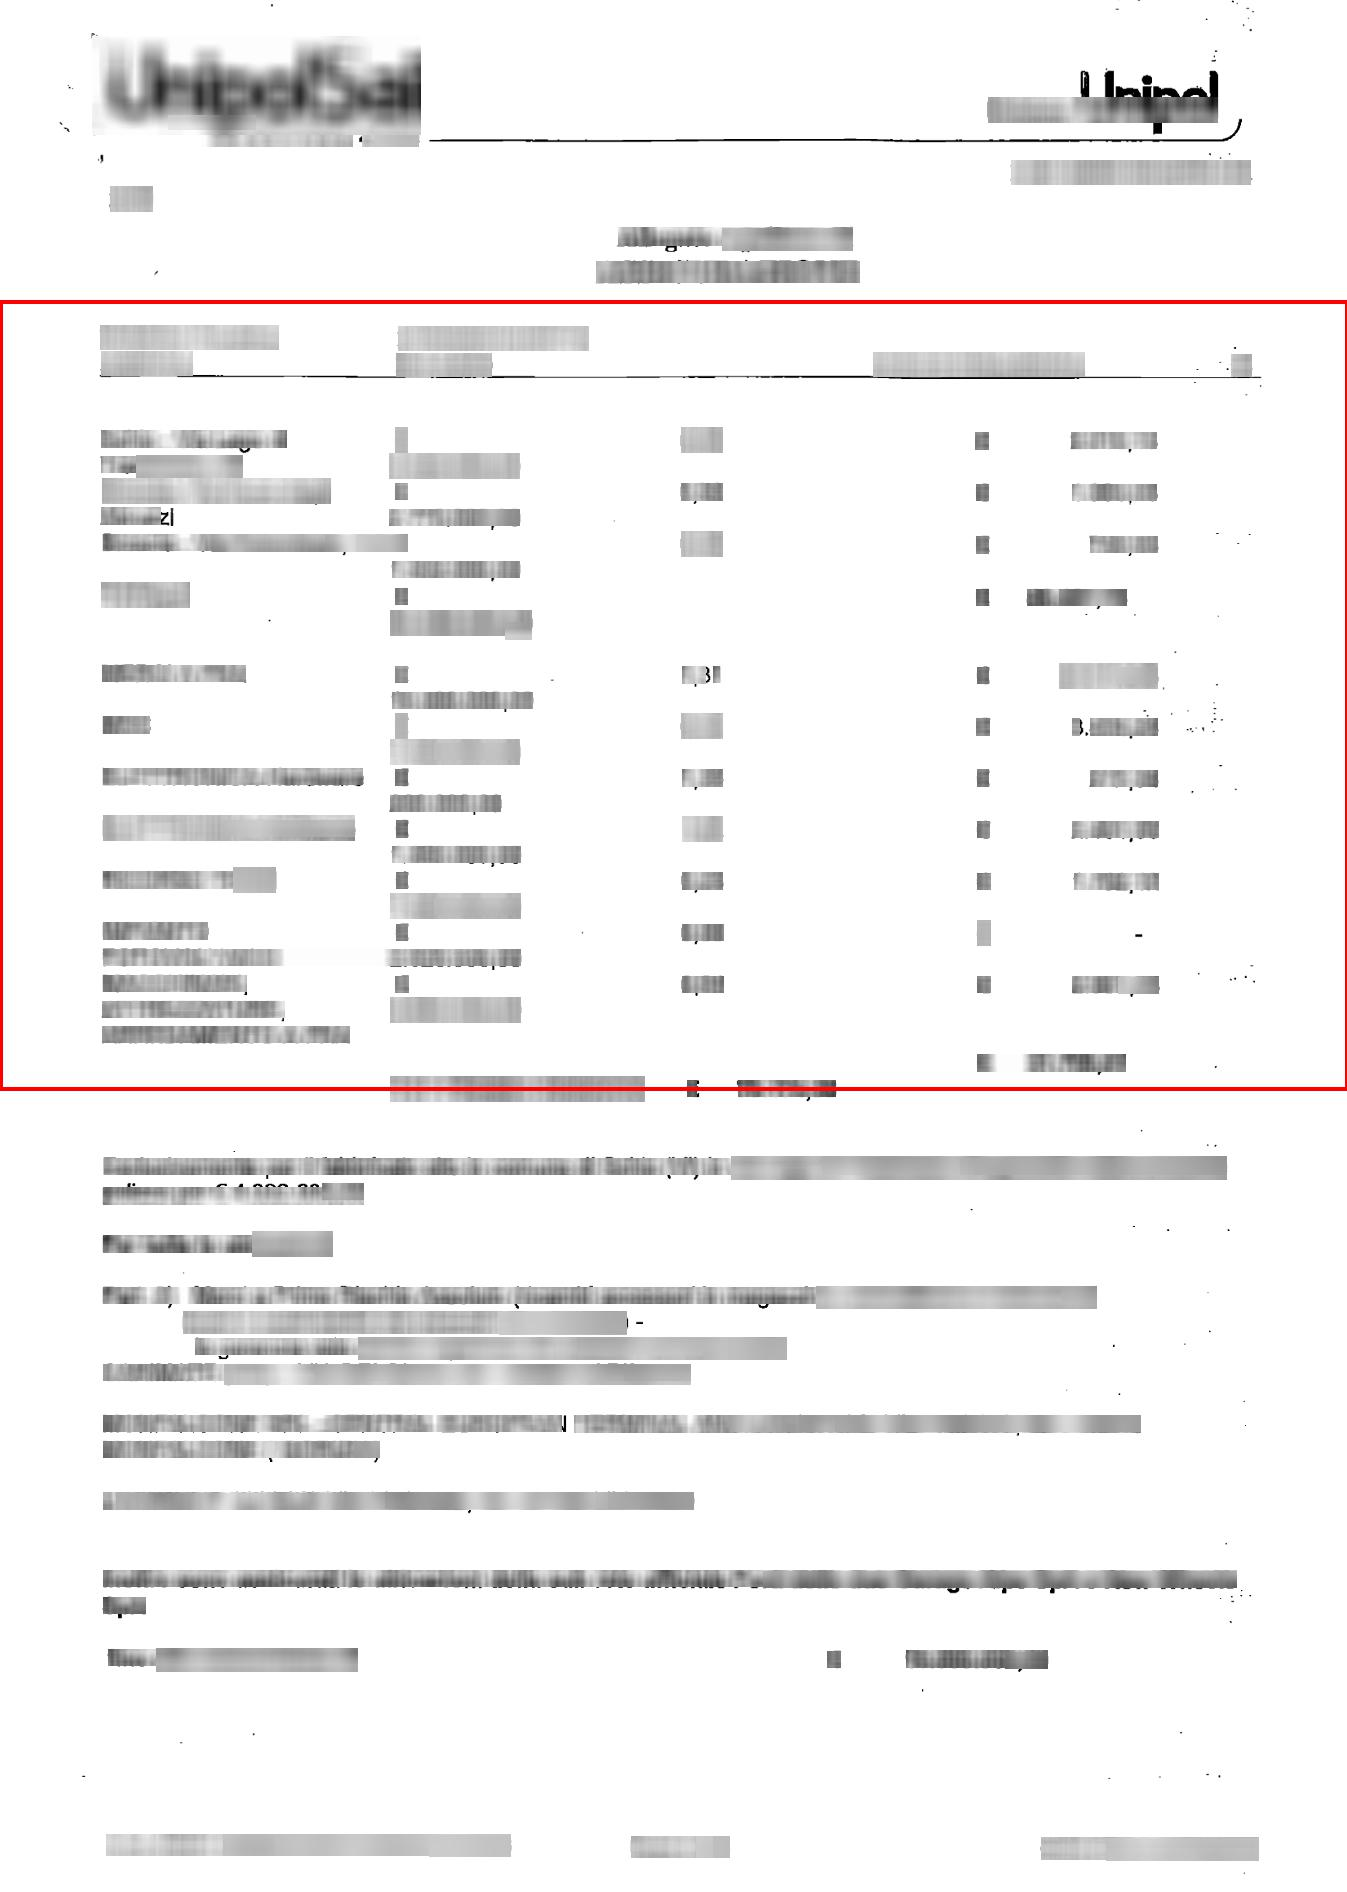
\includegraphics[width=1\columnwidth]{appendice/unite/test0_merged_0_6_momentum_optimizer_1batch}  
    \end{minipage}  
    \caption{Test 0, configurazione 6}
\end{figure}%  
Configurazione:
\begin{multicols}{2}
    \begin{lstlisting}
image_resizer {
  fixes_shape_resizer {
    width: 400
    heigth: 400
  }
}
first_stage_box_predictor {
  l2_regularizer {
    weight: 0.04
}
first_stage_nms_iou_threshold: 0.7
second_stage_box_predictor {
  l2_regularizer {
    weight: 0.004
  }
}
second_stage_post_processing {
  iou_threshold: 0.6
}
batch_size: 1
optimizer {
  adam_optimizer: {
    learning_rate: {
      manual_step_learning_rate {
        initial_learning_rate: 0.0004
        schedule {
          step: 4500
          learning_rate: .0002
        }
        schedule {
          step: 7000
          learning_rate: .00002
        }
        schedule {
          step: 10000
          learning_rate: .000002
        }
    ...
    }
    momentum_optimizer_value: 0.9
  }
  use_moving_average: false
}
    \end{lstlisting}
\end{multicols}
%============================================================================================
\newpage
\subsection{Test 1}
\begin{figure}[!ht] 
    \centering
    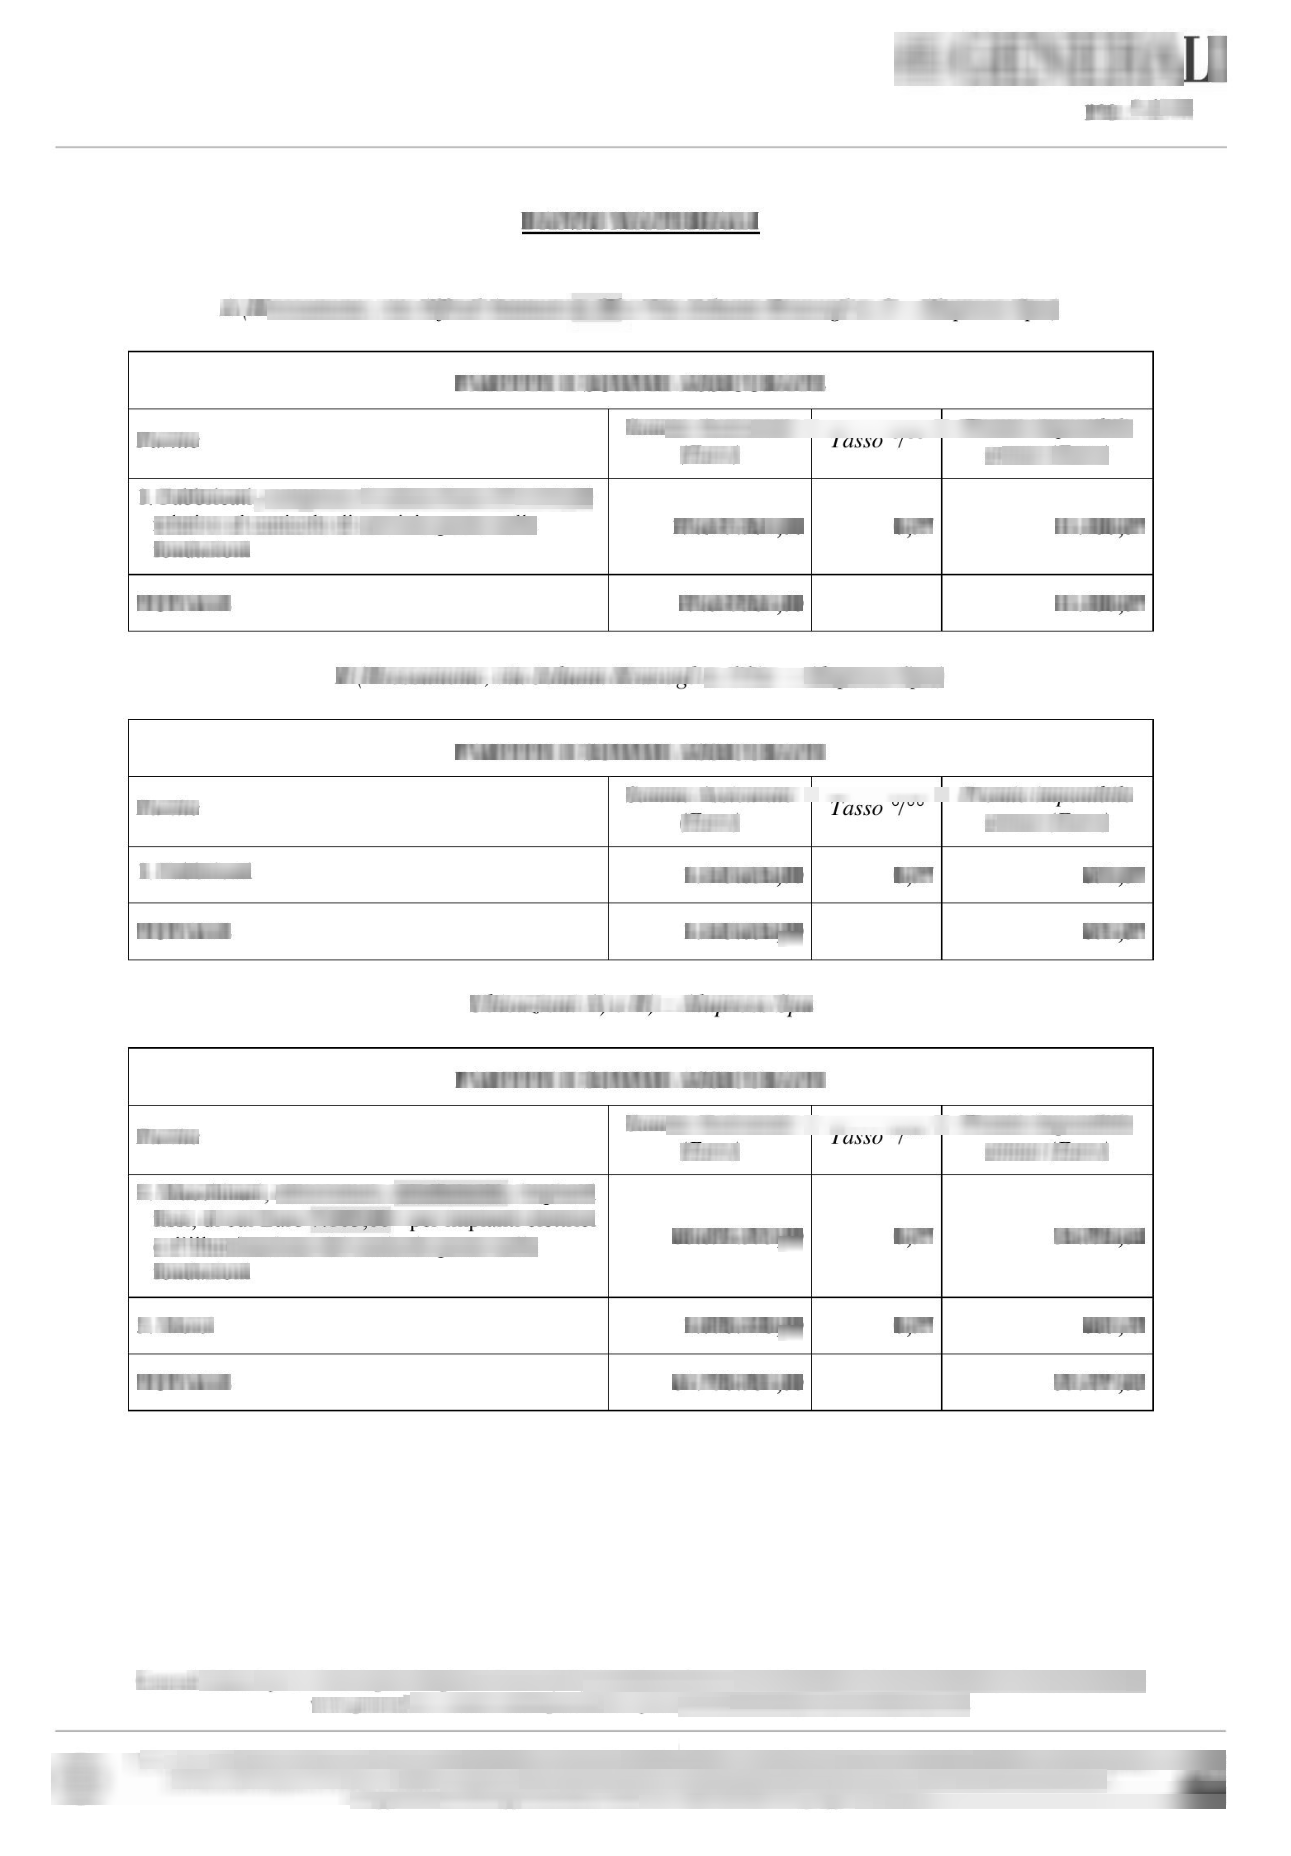
\includegraphics[width=1\columnwidth]{appendice/test1} 
    \caption{Test 1}
    \label{img:test-1}
\end{figure} 
\newpage

%============================================================================================


\begin{figure}[H]  
    \begin{minipage}{.5\columnwidth}  
        \centering  
        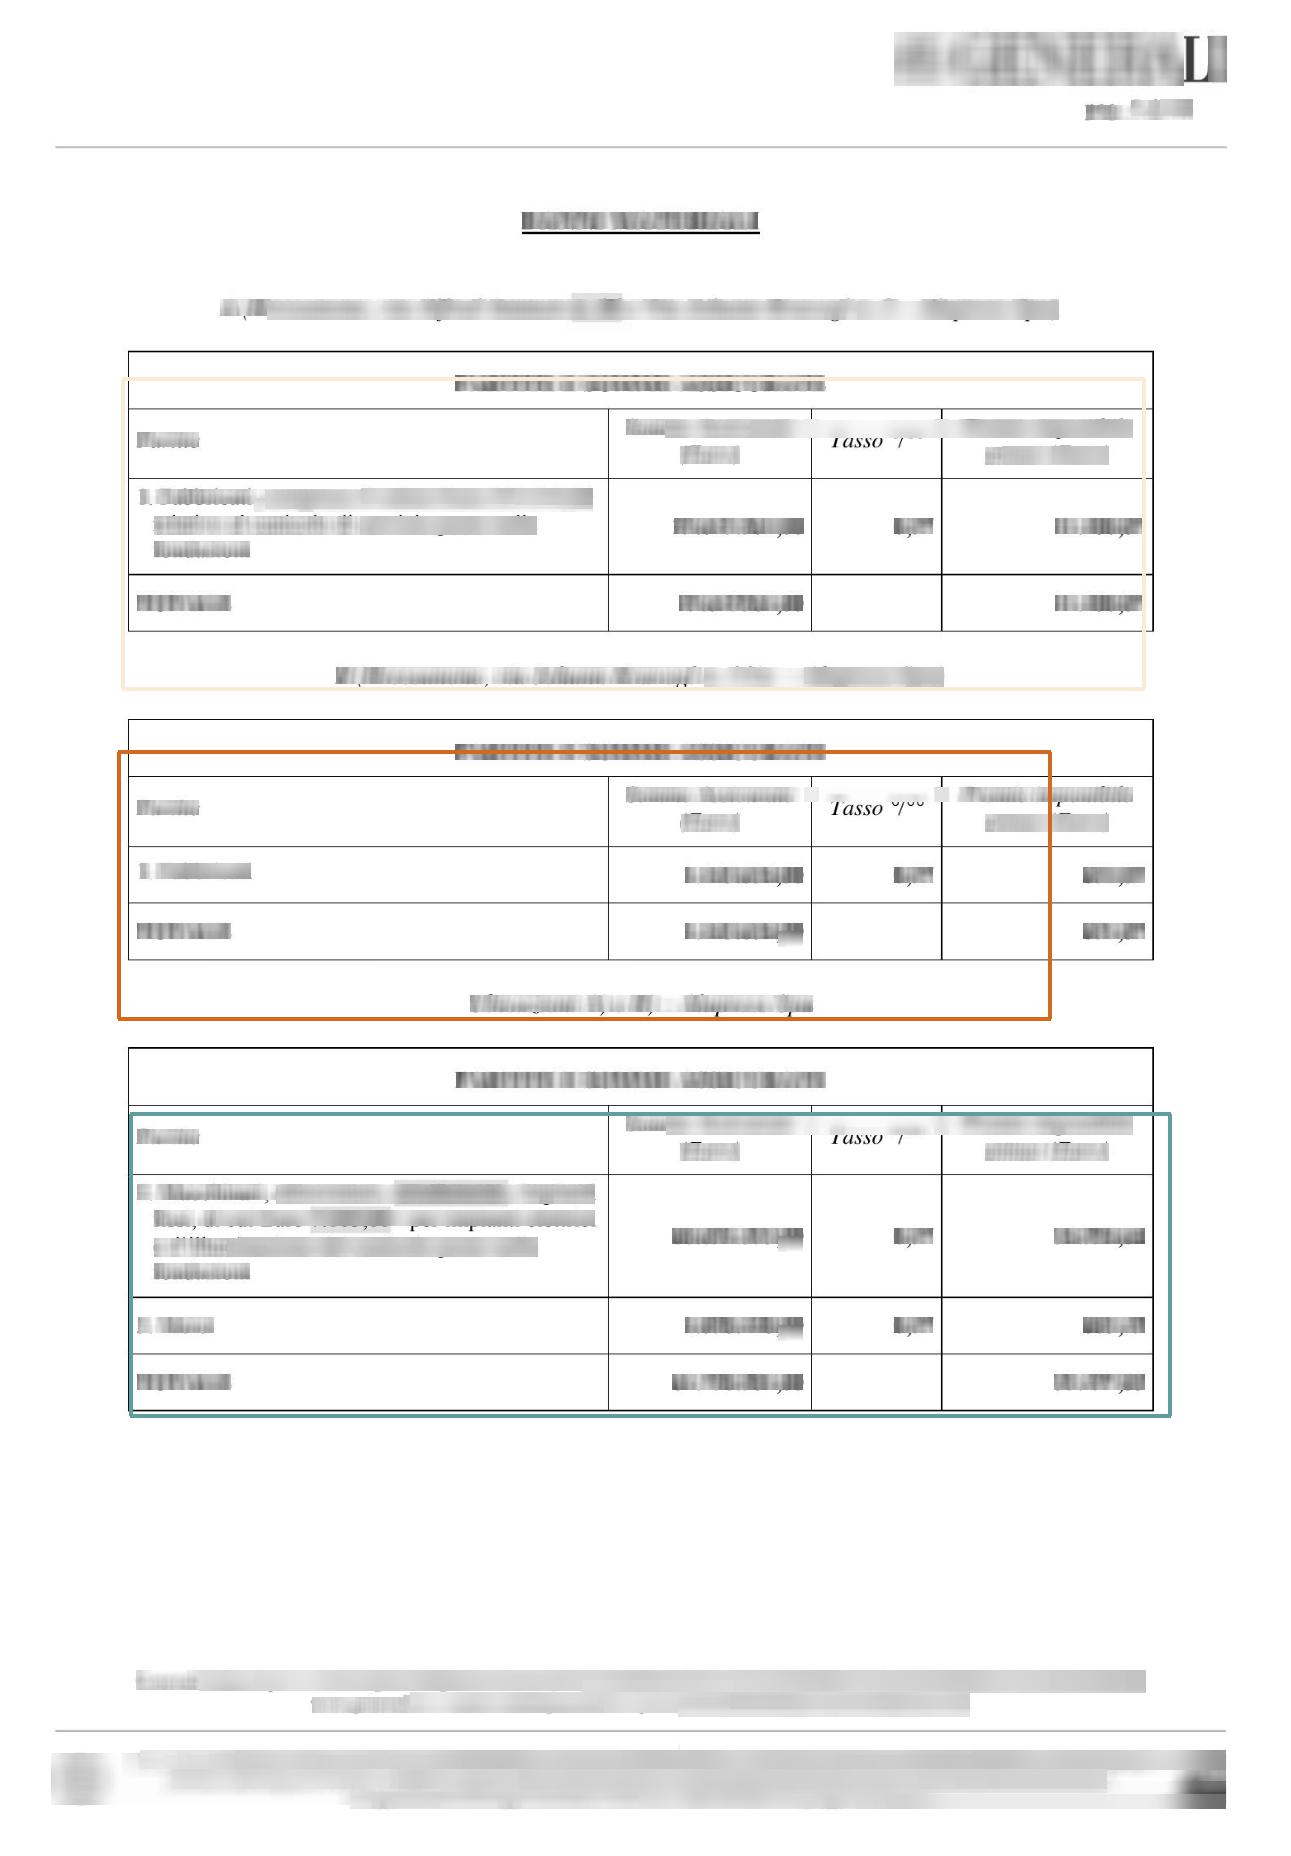
\includegraphics[width=1\columnwidth]{appendice/filtrate/test1_filtered_0_6_adam_1}  
    \end{minipage}%  
    \begin{minipage}{0.5\columnwidth}  
        \centering  
        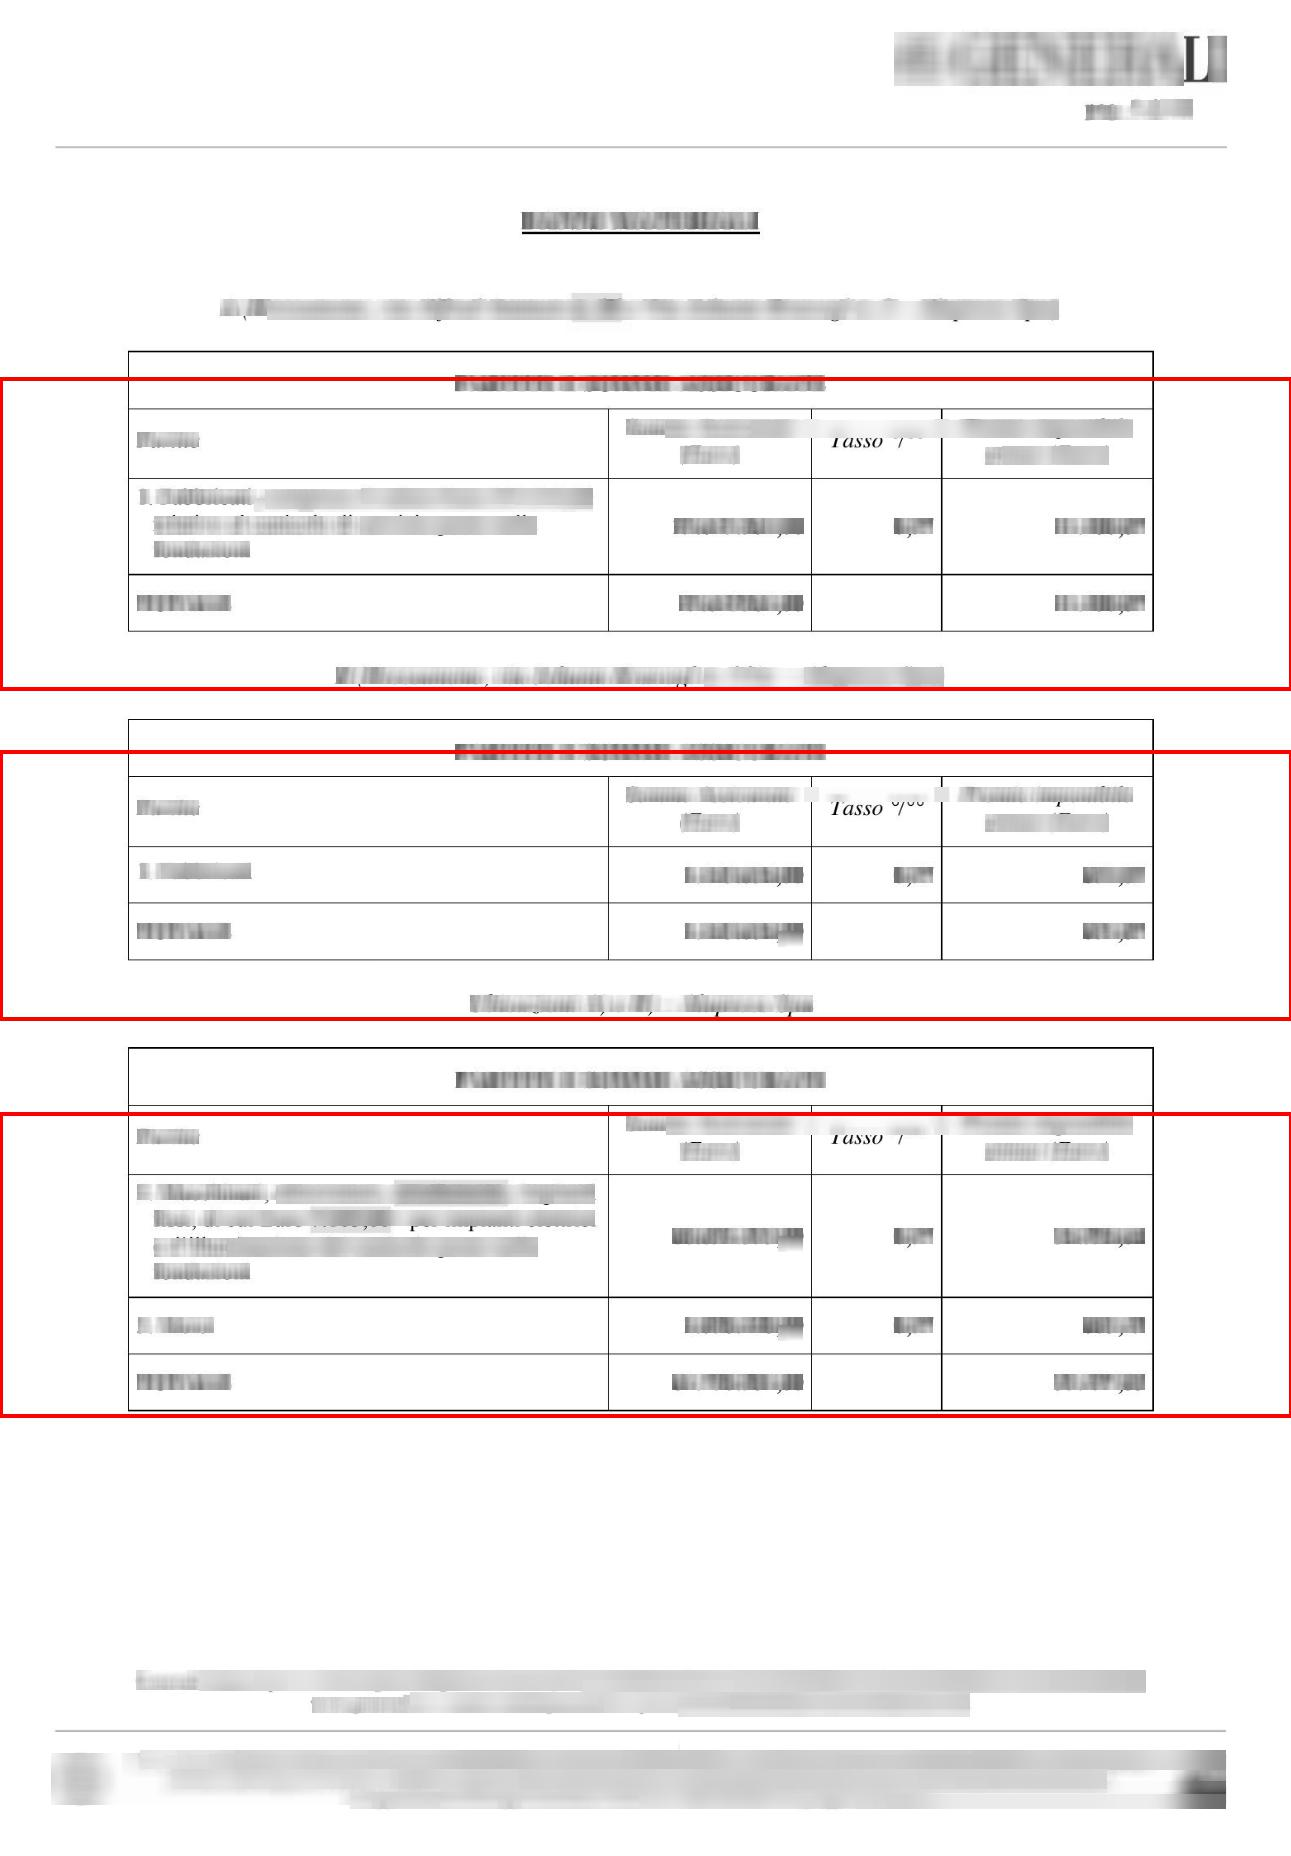
\includegraphics[width=1\columnwidth]{appendice/unite/test1_merged_0_6_adam_1}  
    \end{minipage}  
    \caption{Test 1, configurazione 1}
\end{figure}%  
Configurazione:
\begin{multicols}{2}
    \begin{lstlisting}
image_resizer {
  fixes_shape_resizer {
    width: 400
    heigth: 400
  }
}
first_stage_box_predictor {
  l2_regularizer {
    weight: 0.008
}
first_stage_nms_iou_threshold: 0.7
second_stage_box_predictor {
  l2_regularizer {
    weight: 0.004
  }
}
second_stage_post_processing {
  iou_threshold: 0.6
}
optimizer {
  adam_optimizer: {
    learning_rate: {
      manual_step_learning_rate {
        initial_learning_rate: .00008
        schedule {
          step: 4500
          learning_rate: .00004
        }
        schedule {
          step: 7000
          learning_rate: .00002
        }
        schedule {
          step: 10000
          learning_rate: .000008
        }
    ...
    }
    momentum_optimizer_value: 0.9
  }
  use_moving_average: false
}
\end{lstlisting}
\end{multicols}

%============================================================================================
\newpage
\begin{figure}[H]  
    \begin{minipage}{.5\columnwidth}  
        \centering  
        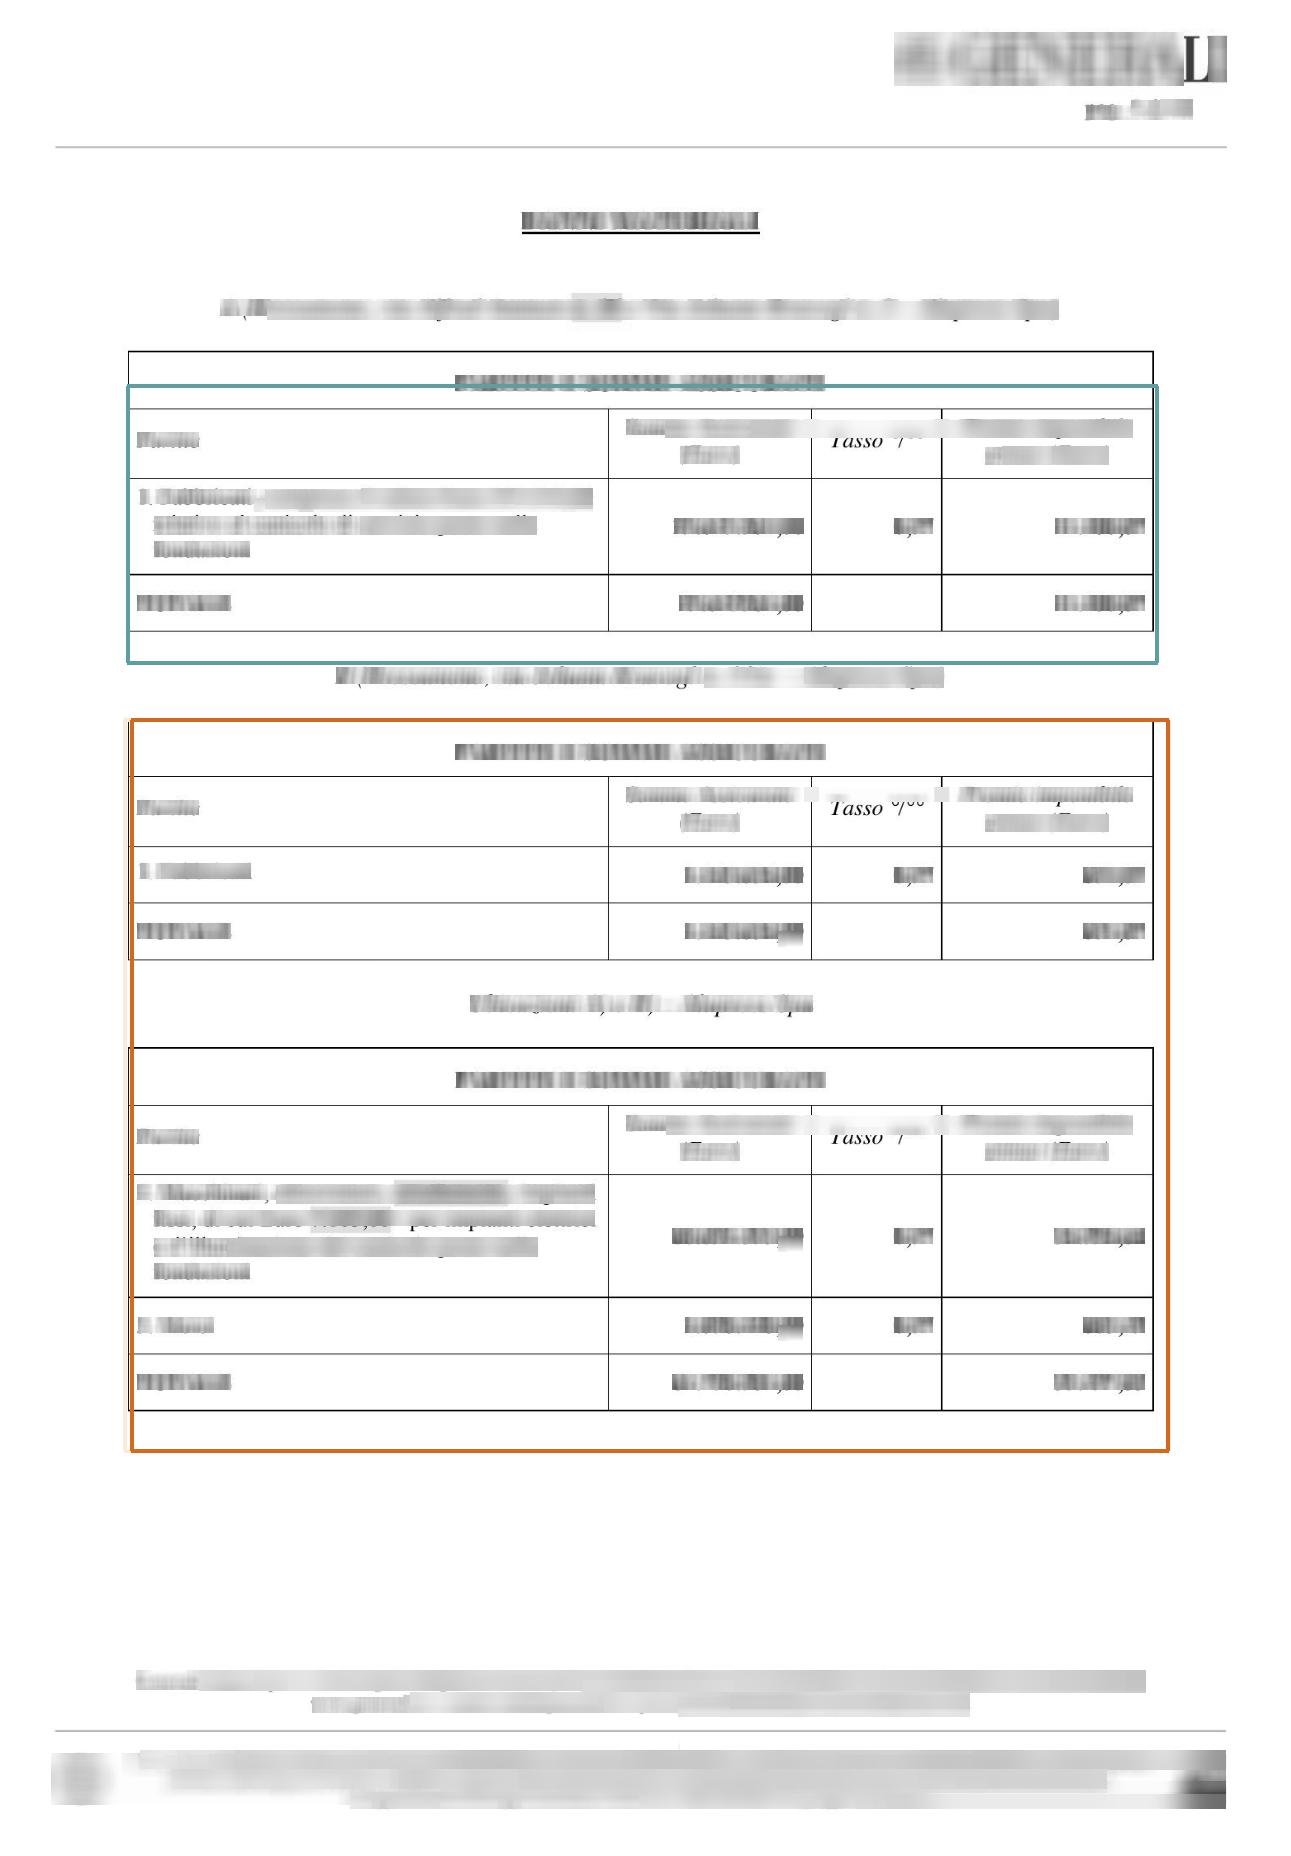
\includegraphics[width=1\columnwidth]{appendice/filtrate/test1_filtered_0_6_adam_3}  
    \end{minipage}%  
    \begin{minipage}{0.5\columnwidth}  
        \centering  
        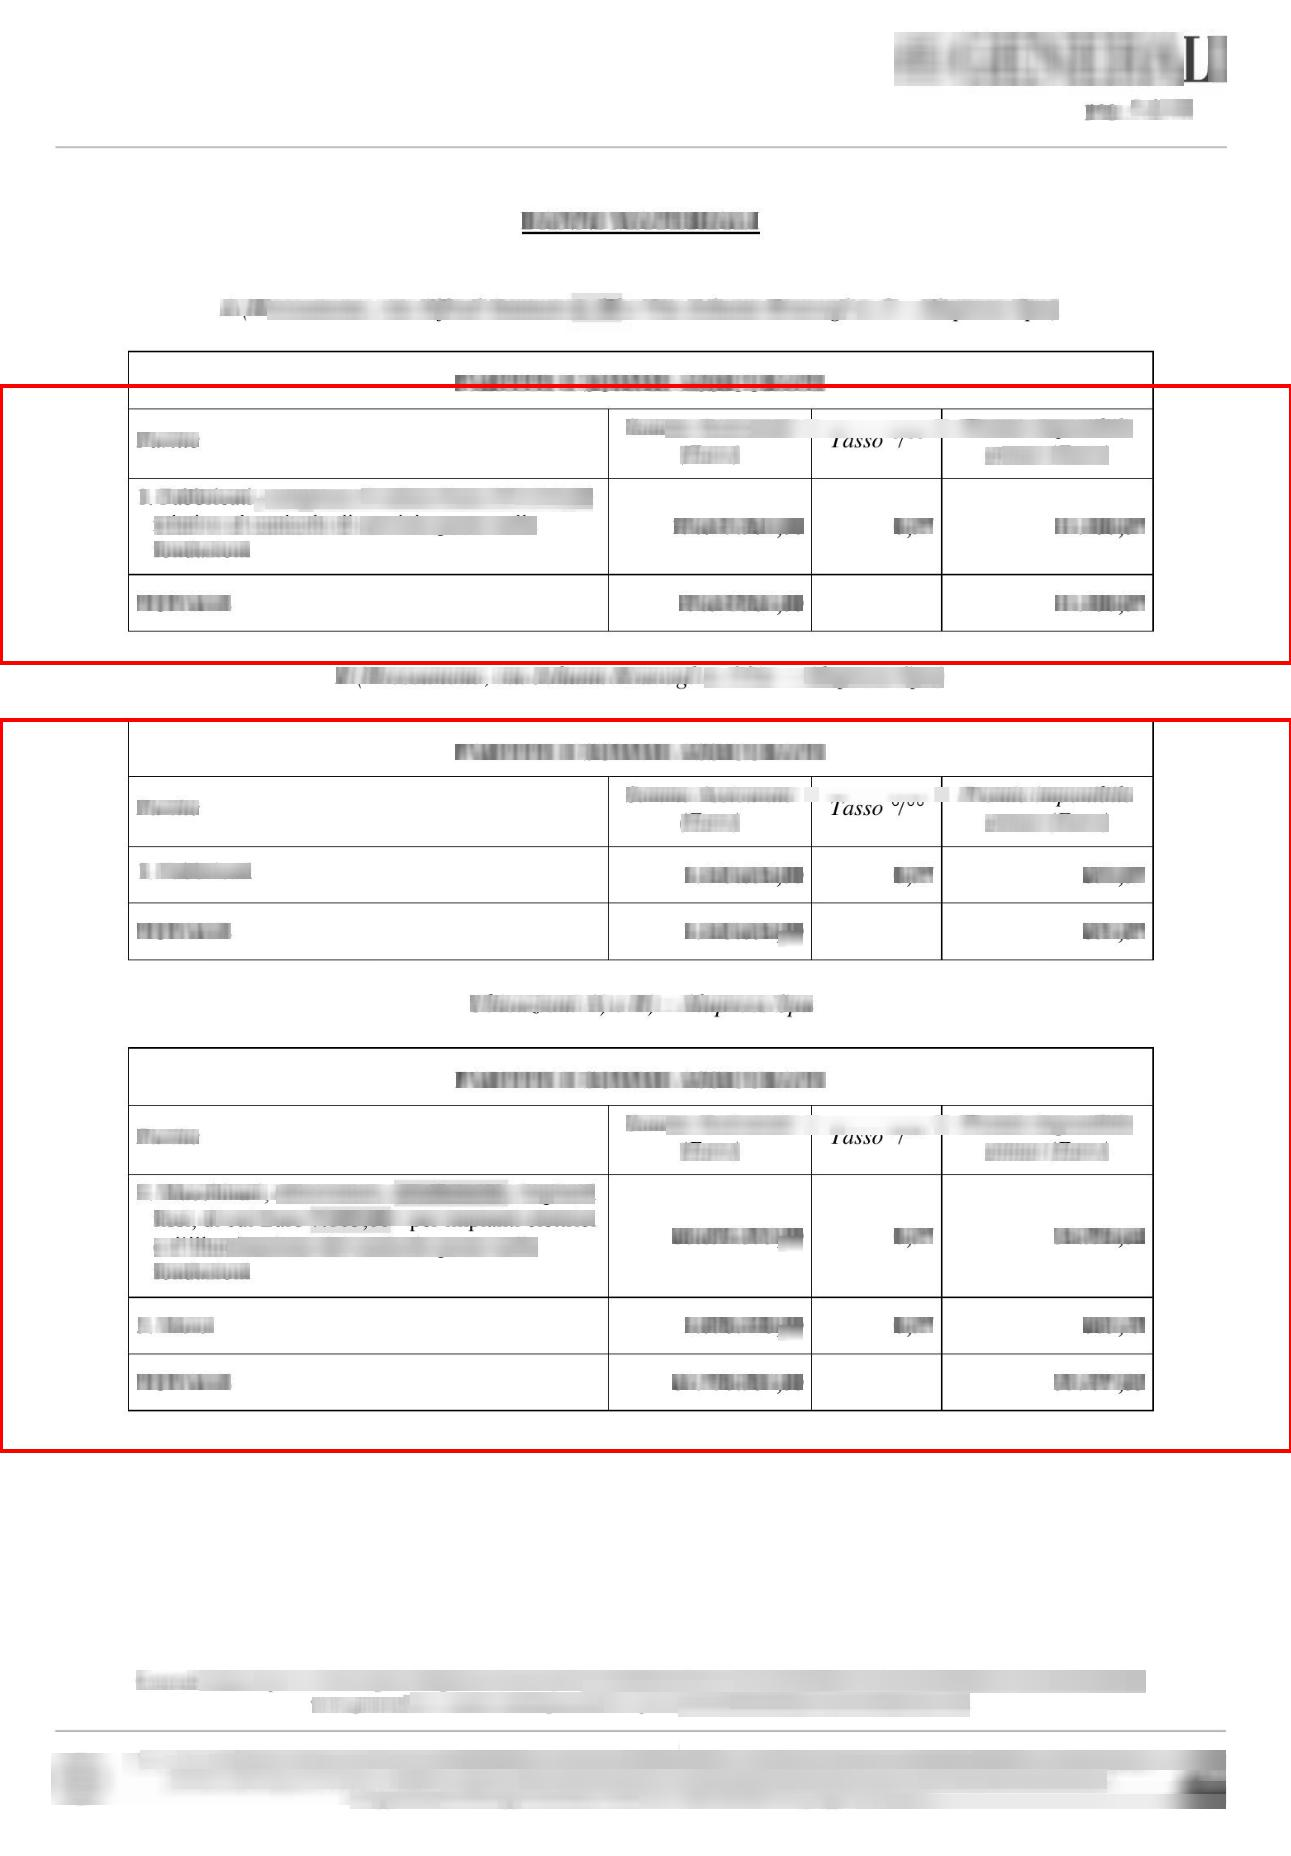
\includegraphics[width=1\columnwidth]{appendice/unite/test1_merged_0_6_adam_3}  
    \end{minipage}  
    \caption{Test 1, configurazione 2}
\end{figure}%  
Configurazione:
\begin{multicols}{2}
    \begin{lstlisting}
image_resizer {
  fixes_shape_resizer {
    width: 400
    heigth: 400
  }
}
first_stage_box_predictor {
  l2_regularizer {
    weight: 0.00001
}
first_stage_nms_iou_threshold: 0.7
second_stage_box_predictor {
  l2_regularizer {
    weight: 0.00004
  }
}
second_stage_post_processing {
  iou_threshold: 0.6
}
optimizer {
  adam_optimizer: {
    learning_rate: {
      exponential_decay_learning_rate {
        initial_learning_rate: 0.0001
          decay_steps: 600
          decay_factor: 0.95
        }
      }
    ...
  use_moving_average: false
}
    \end{lstlisting}
\end{multicols}

%============================================================================================
\newpage
\begin{figure}[H]  
    \begin{minipage}{.5\columnwidth}  
        \centering  
        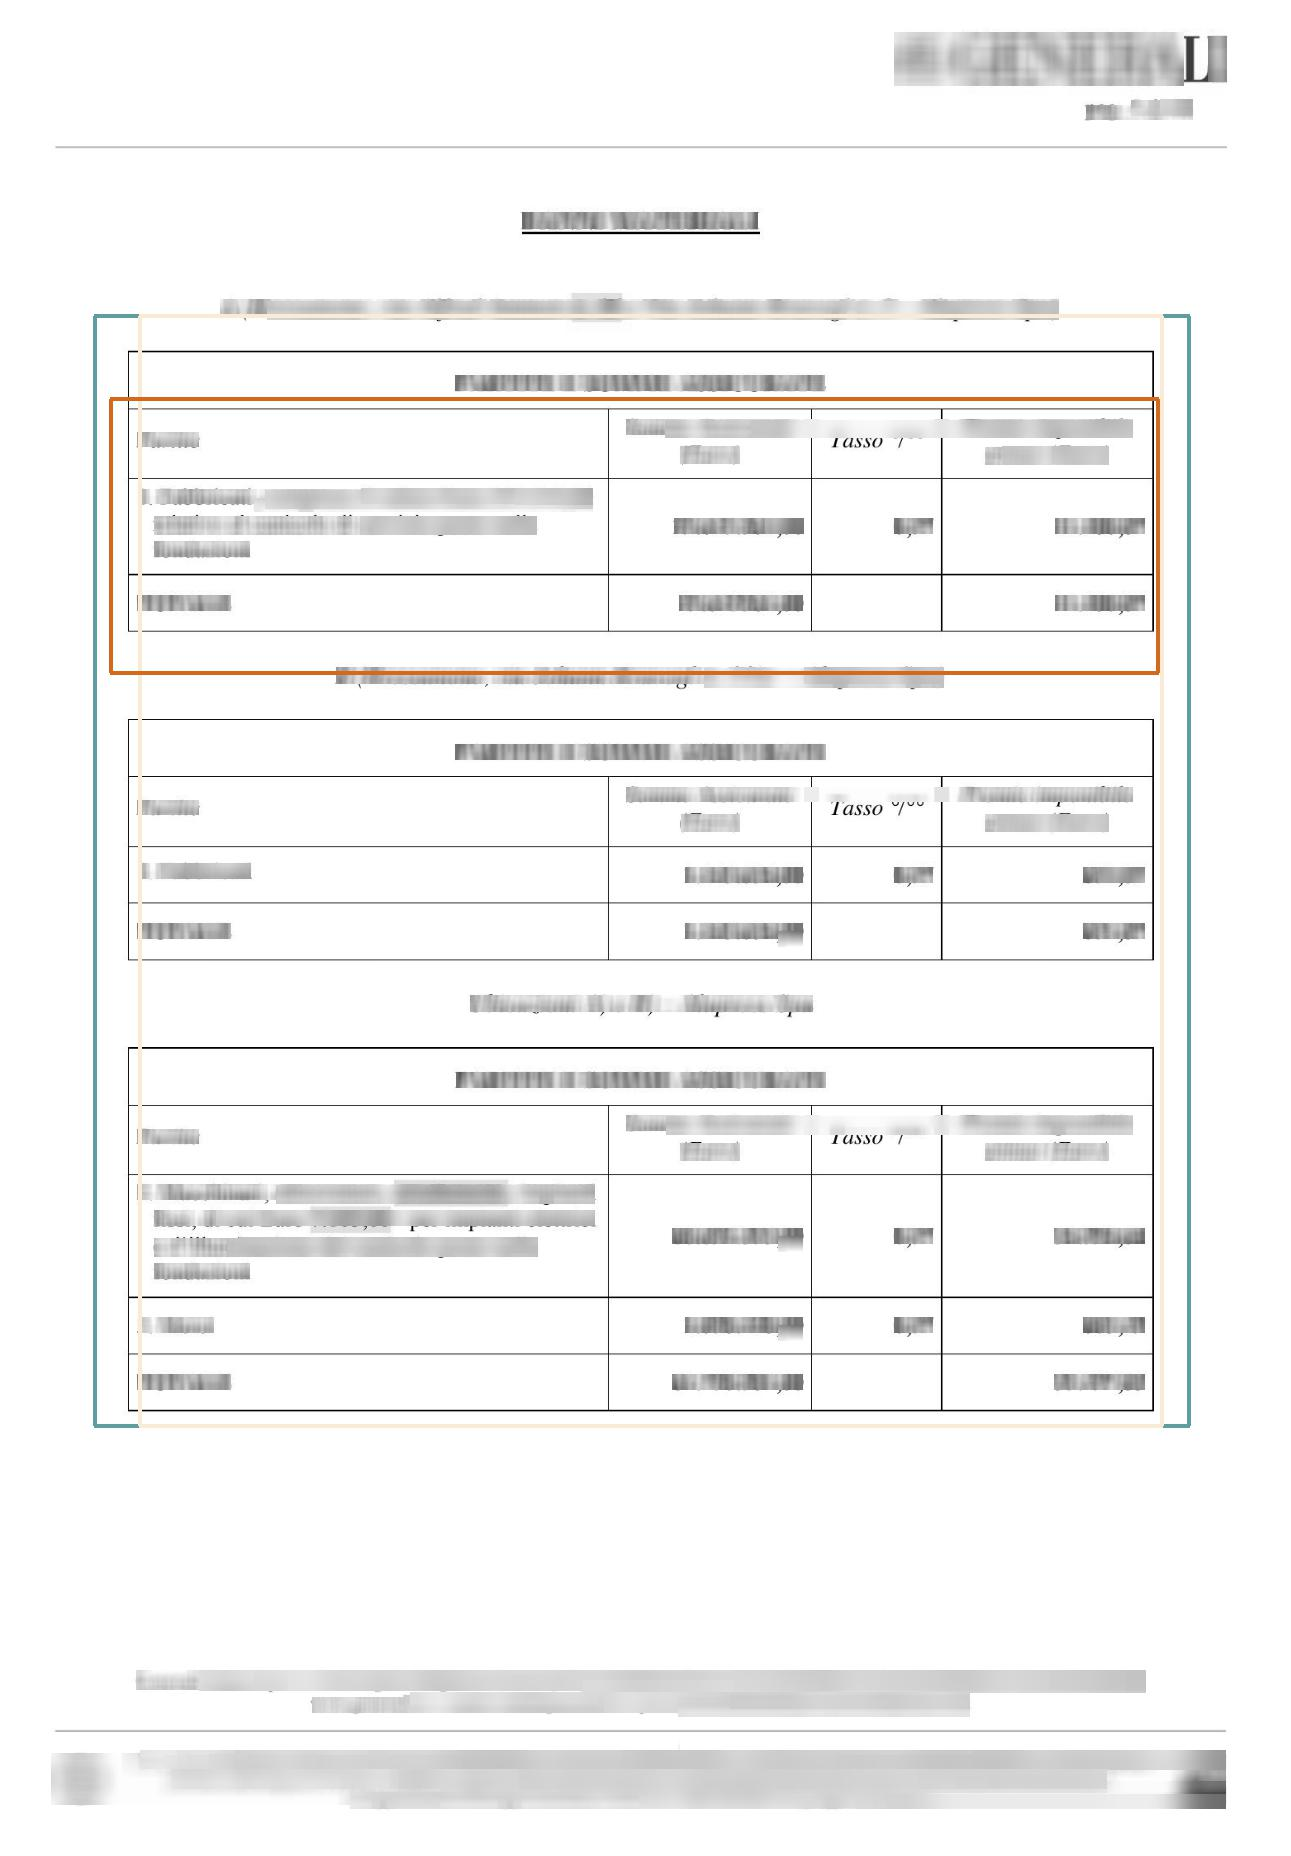
\includegraphics[width=1\columnwidth]{appendice/filtrate/test1_filtered_0_6_adam_4}  
    \end{minipage}%  
    \begin{minipage}{0.5\columnwidth}  
        \centering  
        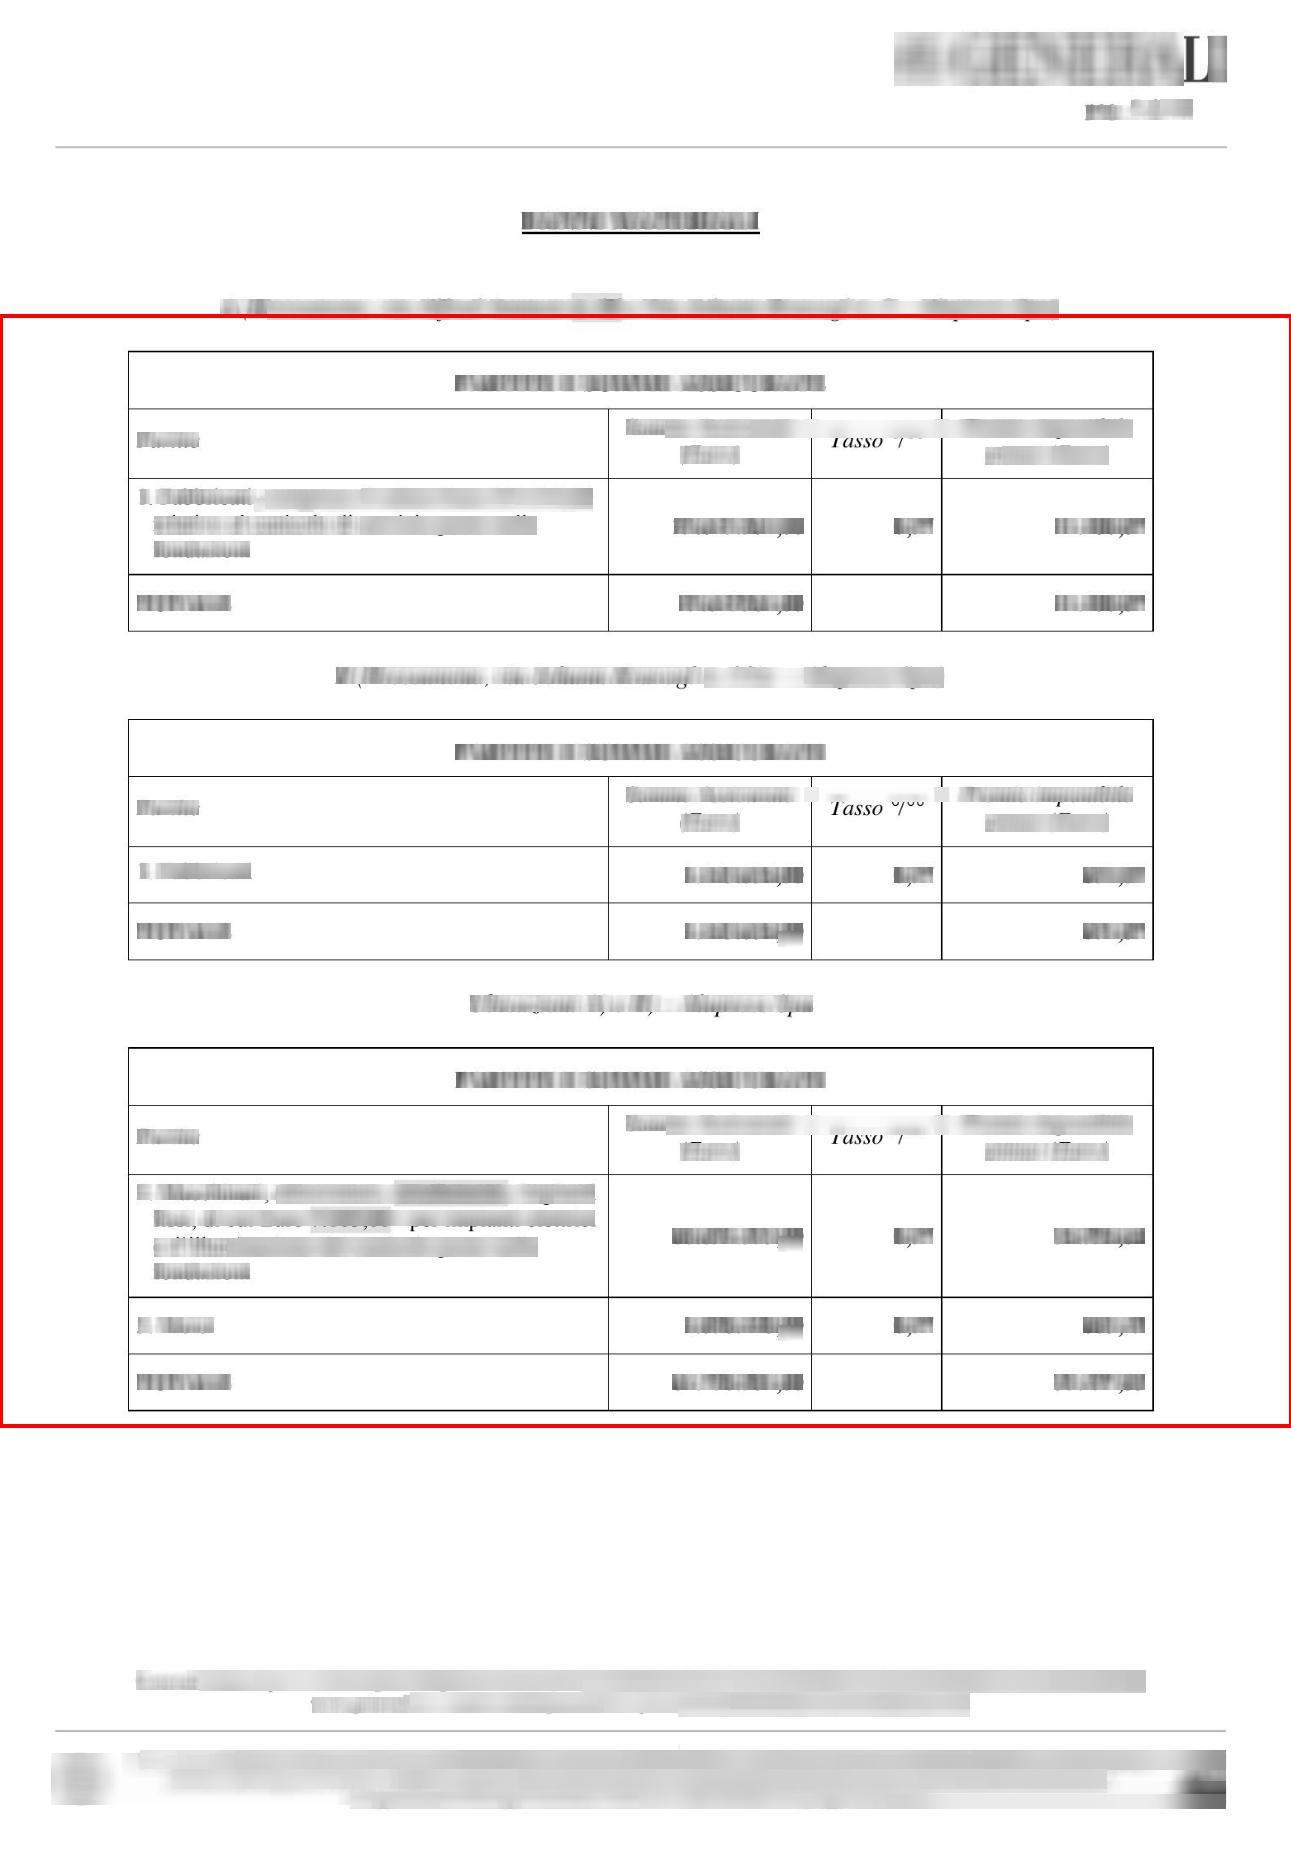
\includegraphics[width=1\columnwidth]{appendice/unite/test1_merged_0_6_adam_4}  
    \end{minipage}  
    \caption{Test 1, configurazione 3}
\end{figure}%  
Configurazione:
\begin{multicols}{2}
    \begin{lstlisting}
image_resizer {
  fixes_shape_resizer {
    width: 400
    heigth: 400
  }
}
first_stage_box_predictor {
  l2_regularizer {
    weight: 0.04
}
first_stage_nms_iou_threshold: 0.7
second_stage_box_predictor {
  l2_regularizer {
    weight: 0.004
  }
}
second_stage_post_processing {
  iou_threshold: 0.6
}
optimizer {
  adam_optimizer: {
    learning_rate: {
      exponential_decay_learning_rate {
        initial_learning_rate: 0.0001
          decay_steps: 450
          decay_factor: 0.9
        }
      }
    ...
  use_moving_average: false
}
    \end{lstlisting}
\end{multicols}

%============================================================================================
\newpage
\begin{figure}[H]  
    \begin{minipage}{.5\columnwidth}  
        \centering  
        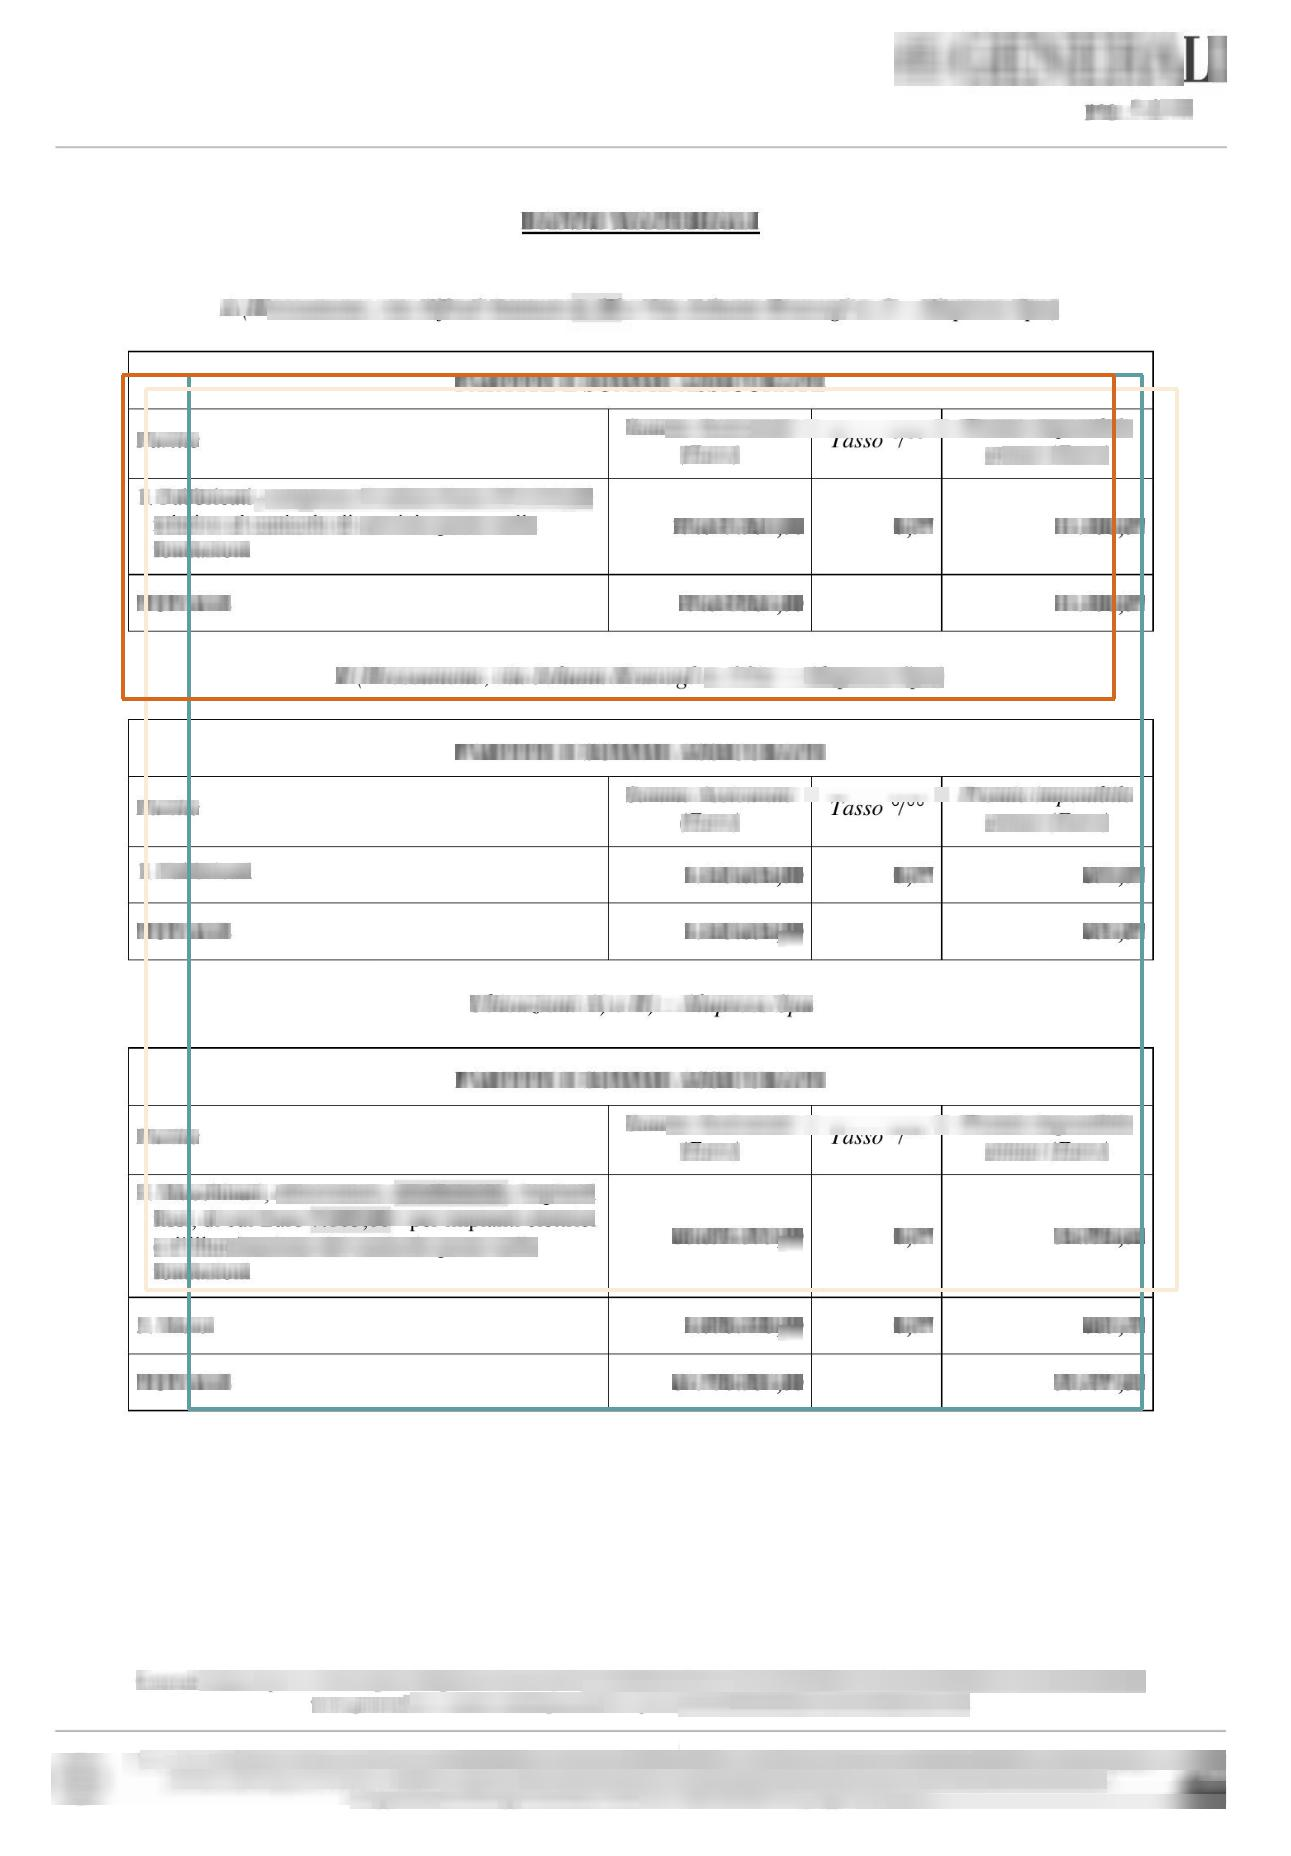
\includegraphics[width=1\columnwidth]{appendice/filtrate/test1_filtered_0_6_momentum_1}  
    \end{minipage}%  
    \begin{minipage}{0.5\columnwidth}  
        \centering  
        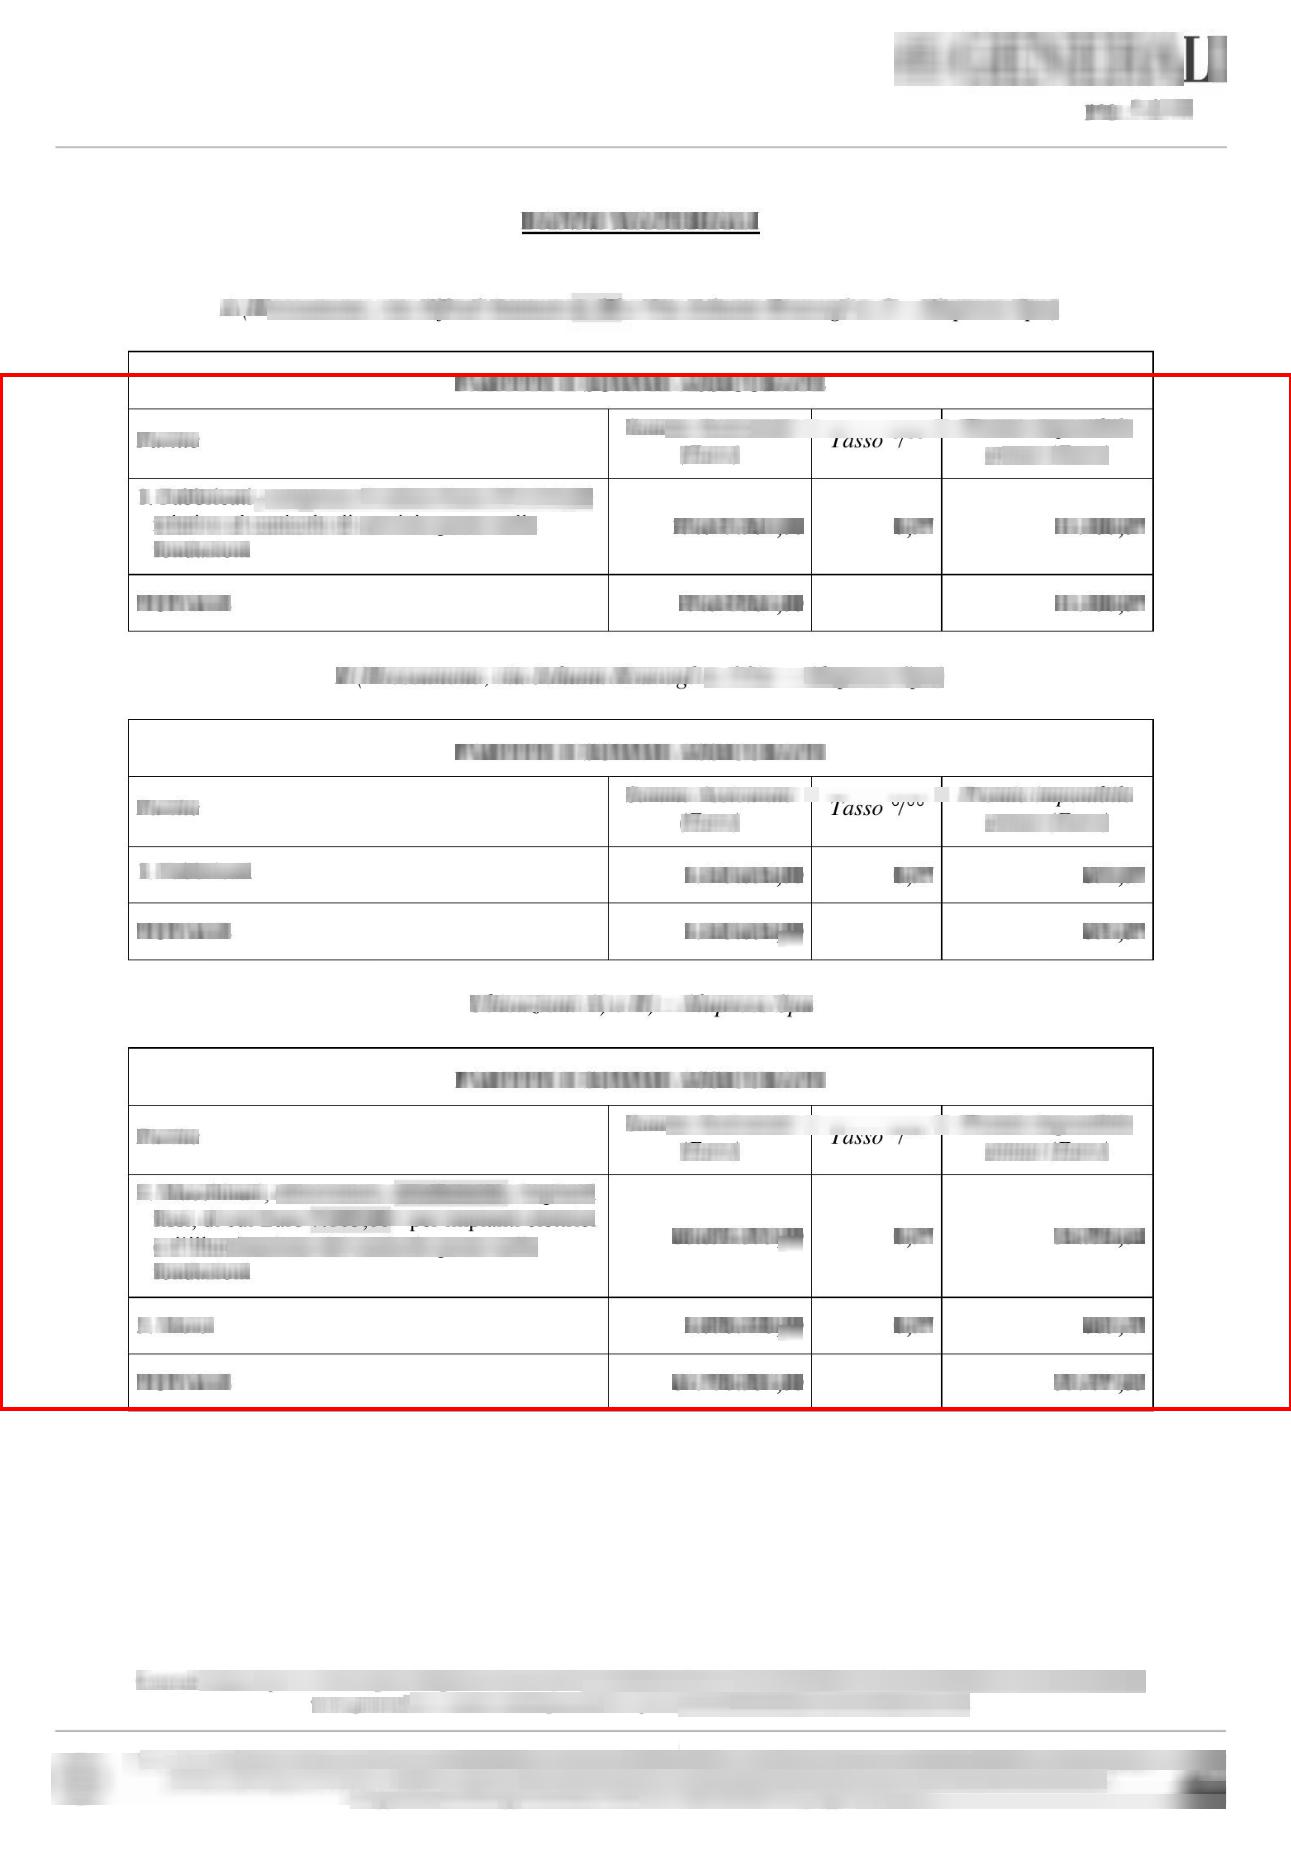
\includegraphics[width=1\columnwidth]{appendice/unite/test1_merged_0_6_momentum_1}  
    \end{minipage}  
    \caption{Test 1, configurazione 4}
\end{figure}%  
Configurazione:
\begin{multicols}{2}
    \begin{lstlisting}
image_resizer {
  fixes_shape_resizer {
    width: 400
    heigth: 400
  }
}
first_stage_box_predictor {
  l2_regularizer {
    weight: 0.00001
}
first_stage_nms_iou_threshold: 0.7
second_stage_box_predictor {
  l2_regularizer {
    weight: 0.00004
  }
}
second_stage_post_processing {
  iou_threshold: 0.6
}
optimizer {
  adam_optimizer: {
    learning_rate: {
      manual_step_learning_rate {
        initial_learning_rate: 0.0008
        schedule {
          step: 4500
          learning_rate: .0008
        }
        schedule {
          step: 7000
          learning_rate: .0004
        }
        schedule {
          step: 10000
          learning_rate: .00008
        }
    ...
    }
    momentum_optimizer_value: 0.9
  }
  use_moving_average: false
}
    \end{lstlisting}
\end{multicols}
%============================================================================================

\newpage
\begin{figure}[H]  
    \begin{minipage}{.5\columnwidth}  
        \centering  
        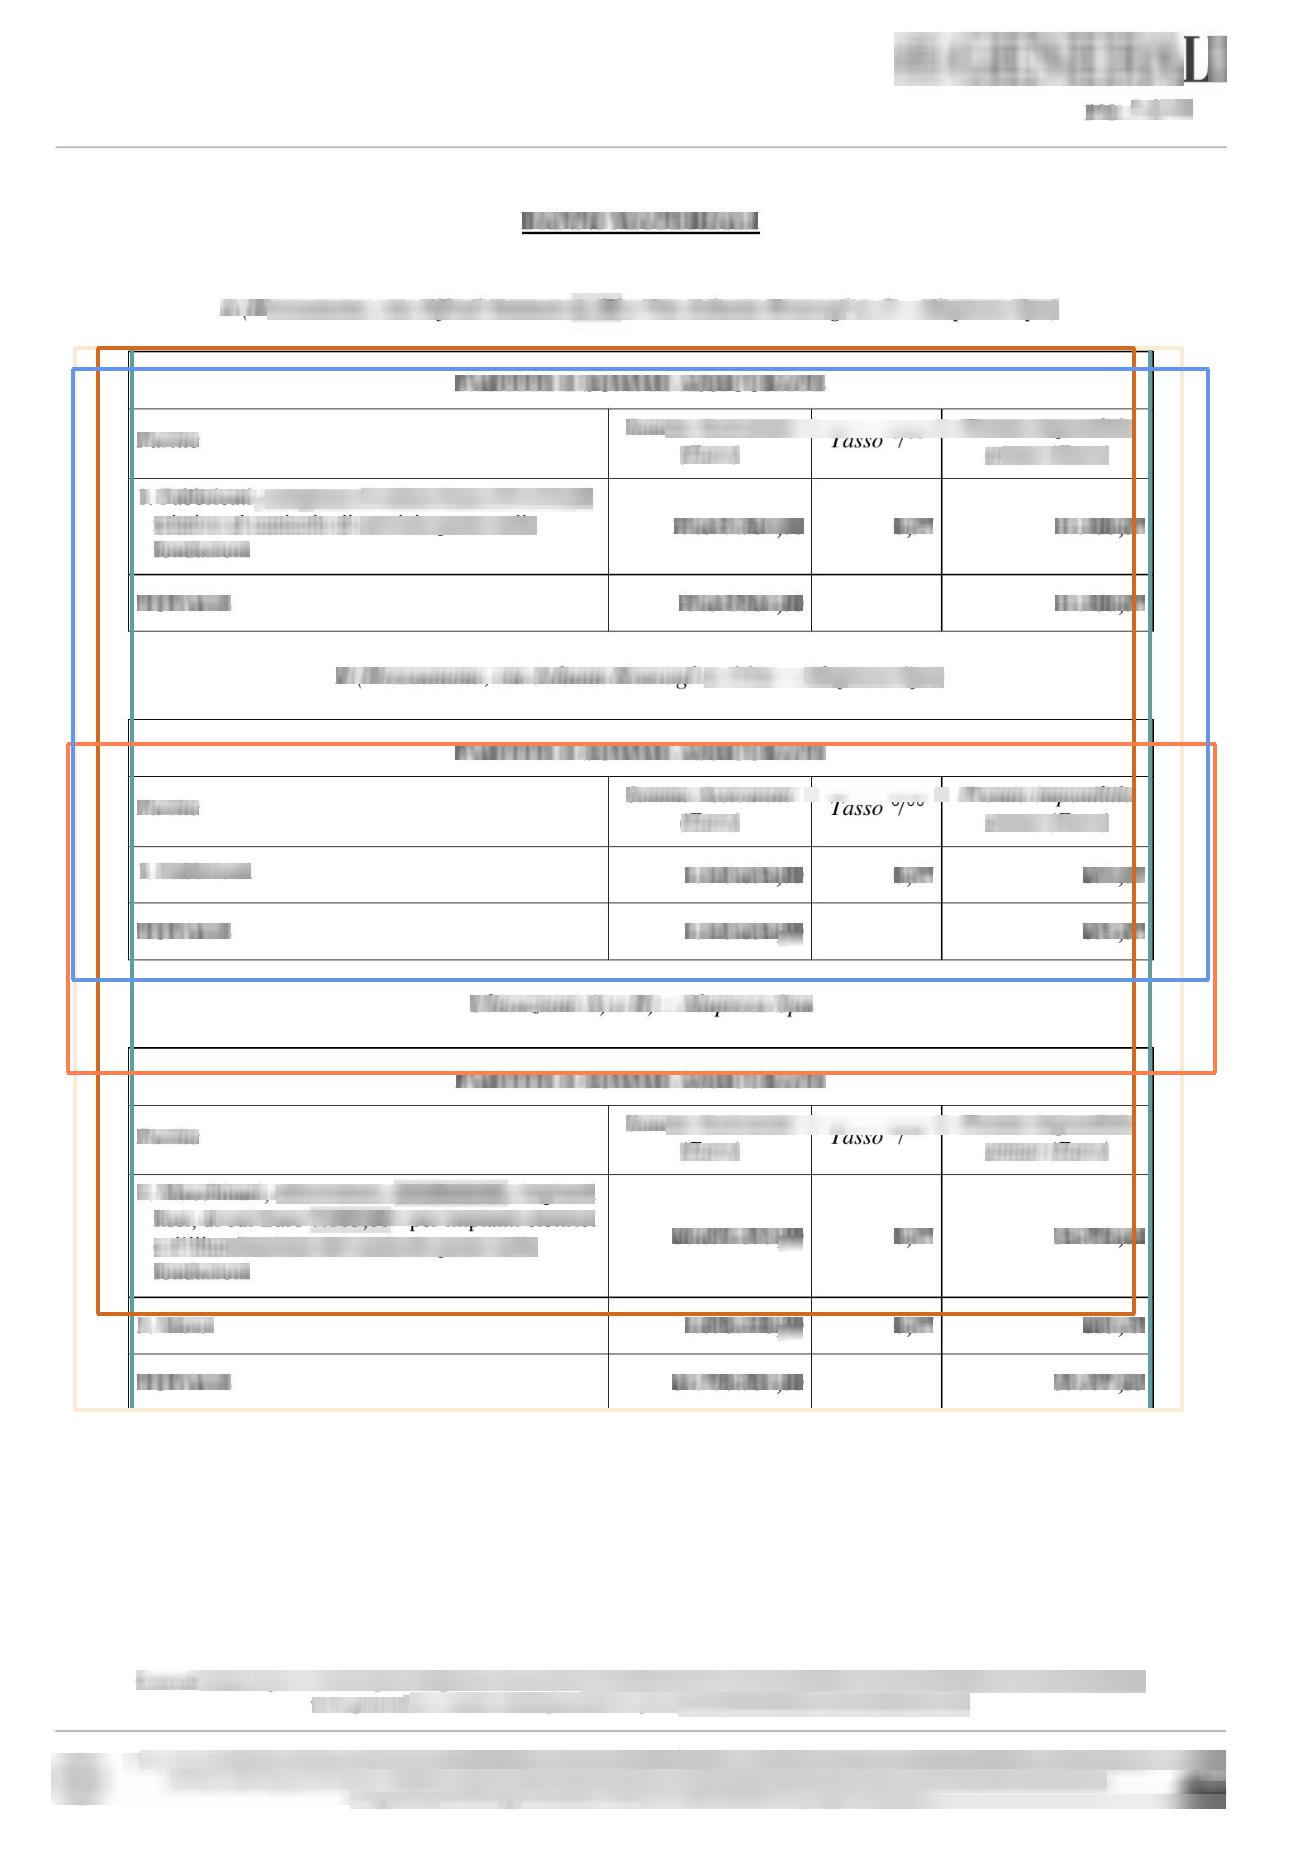
\includegraphics[width=1\columnwidth]{appendice/filtrate/test1_filtered_0_6_momentum_10k_jpg}  
    \end{minipage}%  
    \begin{minipage}{0.5\columnwidth}  
        \centering  
        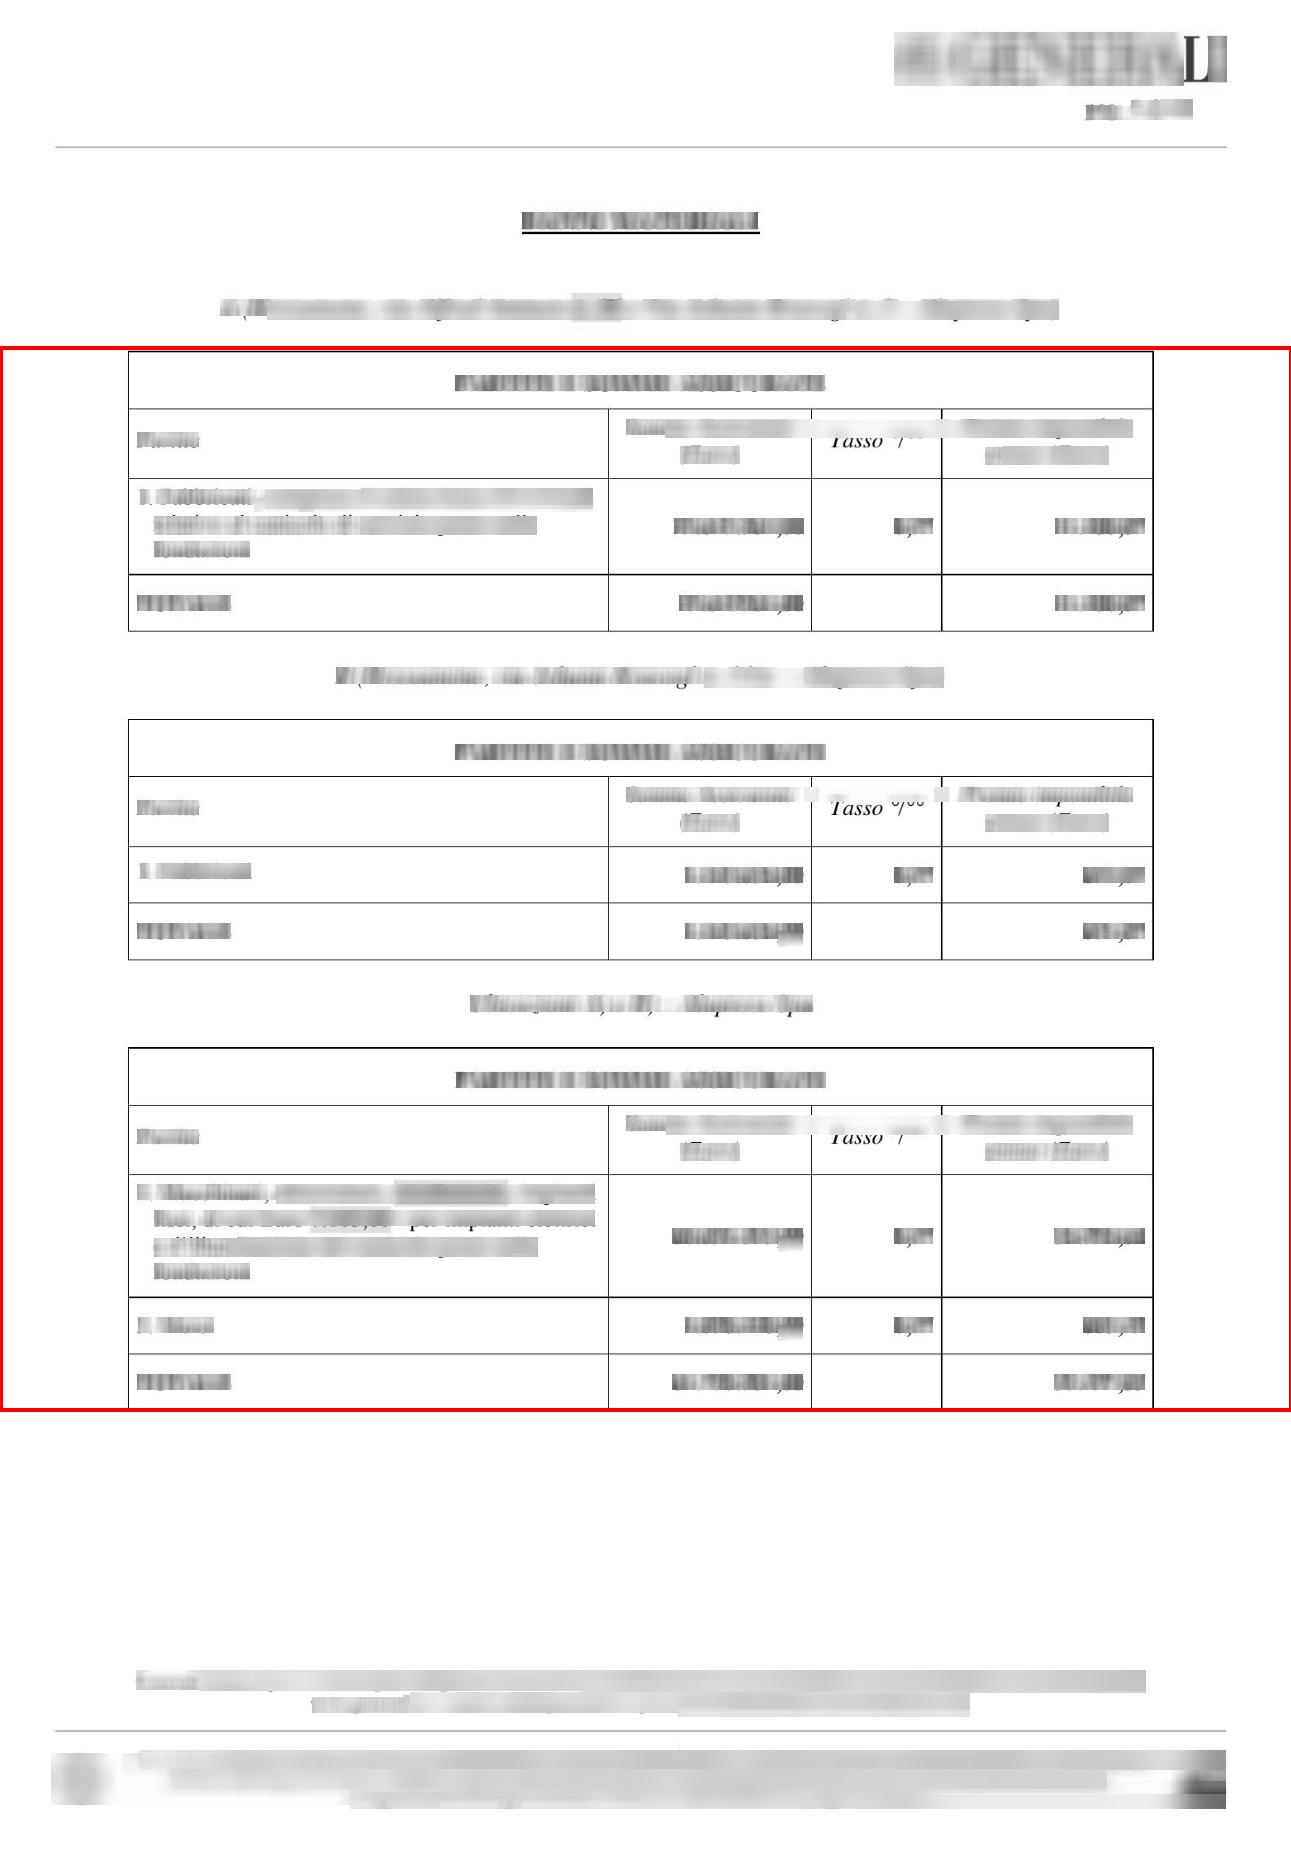
\includegraphics[width=1\columnwidth]{appendice/unite/test1_merged_0_6_momentum_10k_jpg}  
    \end{minipage}  
    \caption{Test 1, configurazione 5}
\end{figure}%  
Configurazione:
\begin{multicols}{2}
    \begin{lstlisting}
image_resizer {
  fixes_shape_resizer {
    width: 400
    heigth: 400
  }
}
first_stage_box_predictor {
  l2_regularizer {
    weight: 0.004
}
first_stage_nms_iou_threshold: 0.7
second_stage_box_predictor {
  l2_regularizer {
    weight: 0.004
  }
}
second_stage_post_processing {
  iou_threshold: 0.6
}
optimizer {
  adam_optimizer: {
    learning_rate: {
      manual_step_learning_rate {
        initial_learning_rate: 0.0004
        schedule {
          step: 4500
          learning_rate: .0002
        }
        schedule {
          step: 7000
          learning_rate: .00002
        }
        schedule {
          step: 10000
          learning_rate: .000002
        }
    ...
    }
    momentum_optimizer_value: 0.9
  }
  use_moving_average: false
}
    \end{lstlisting}
\end{multicols}
%============================================================================================

\newpage
\begin{figure}[H]  
    \begin{minipage}{.5\columnwidth}  
        \centering  
        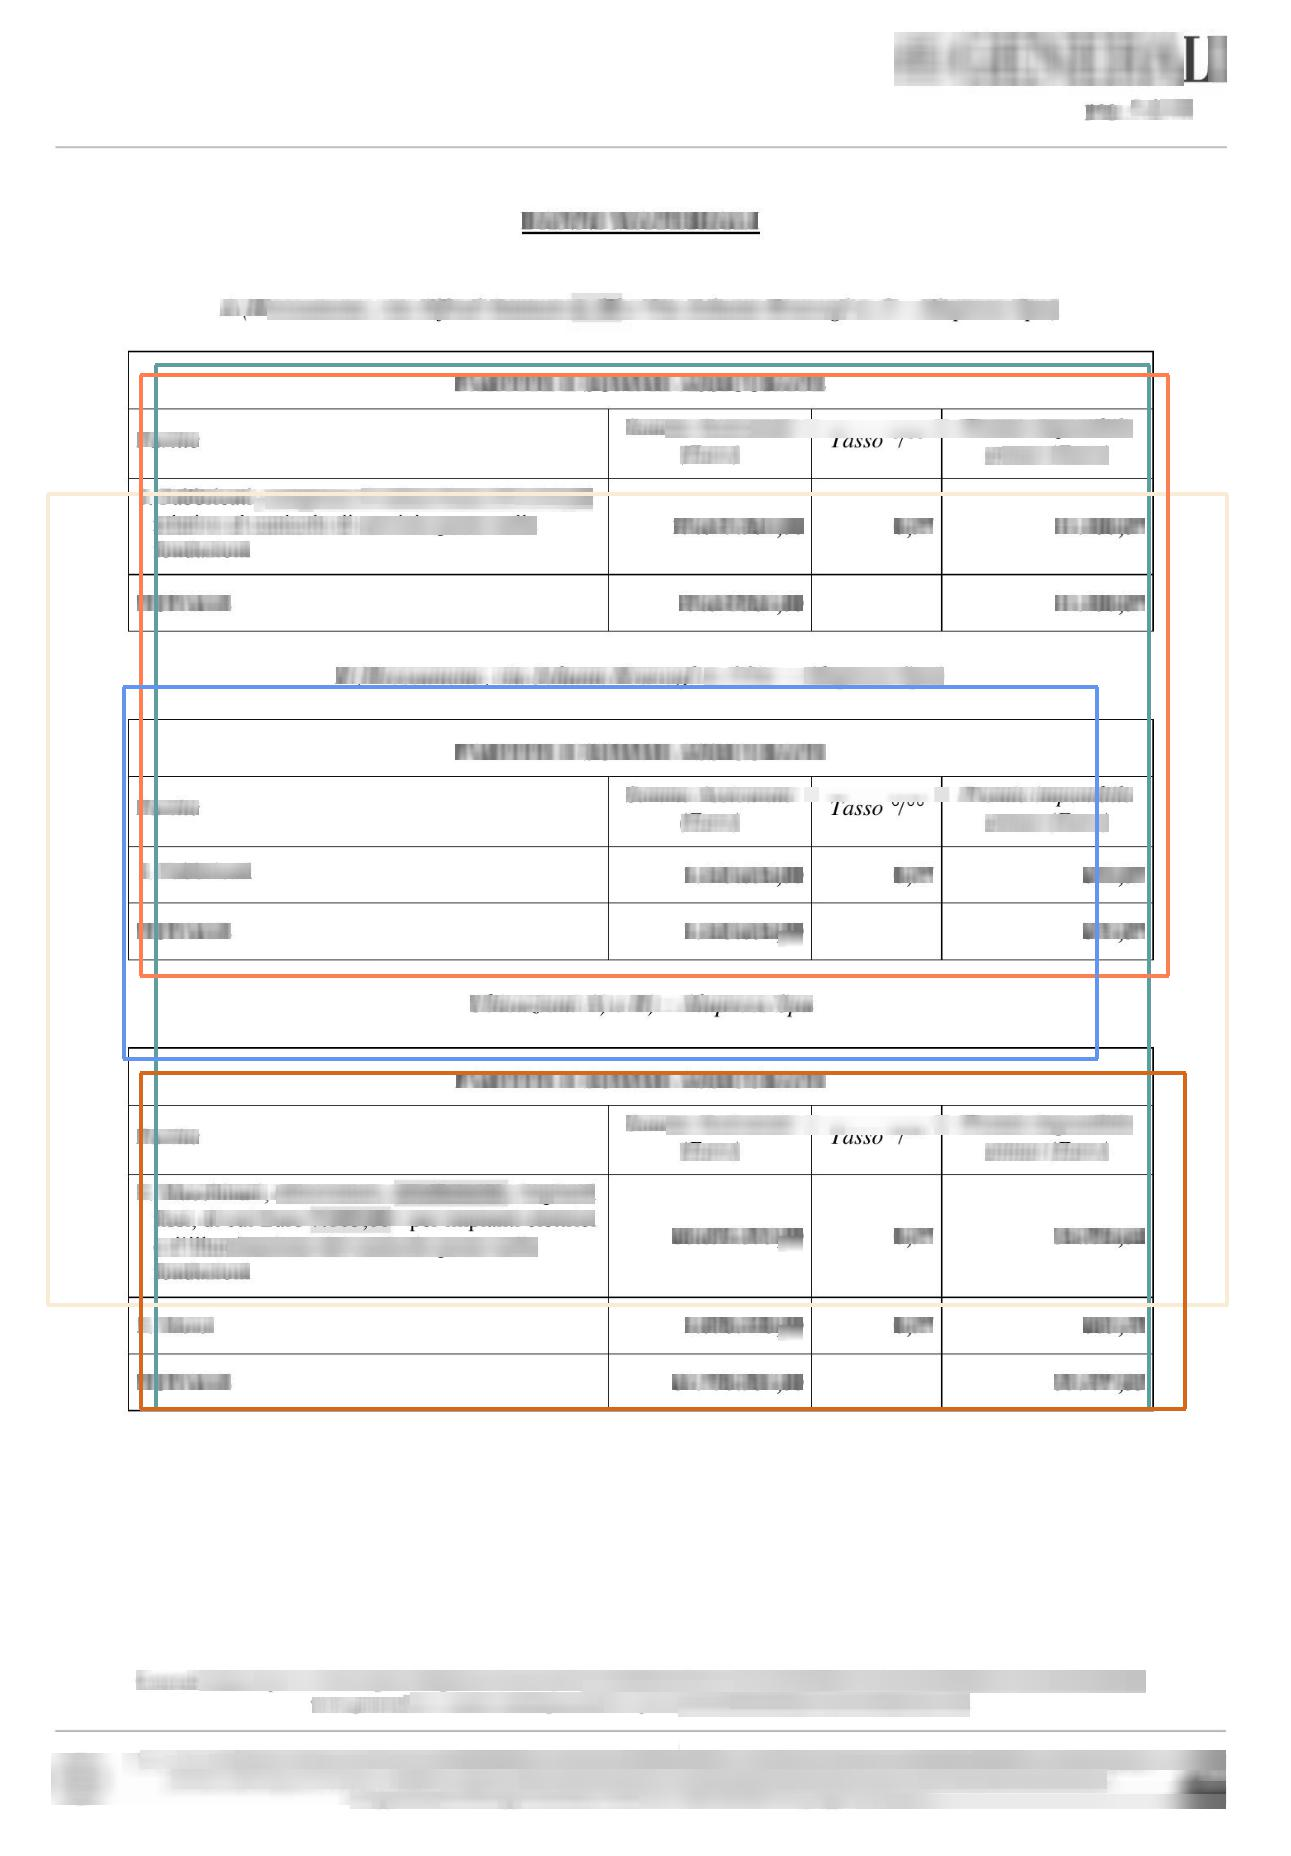
\includegraphics[width=1\columnwidth]{appendice/filtrate/test1_filtered_0_6_momentum_optimizer_1batch}  
    \end{minipage}%  
    \begin{minipage}{0.5\columnwidth}  
        \centering  
        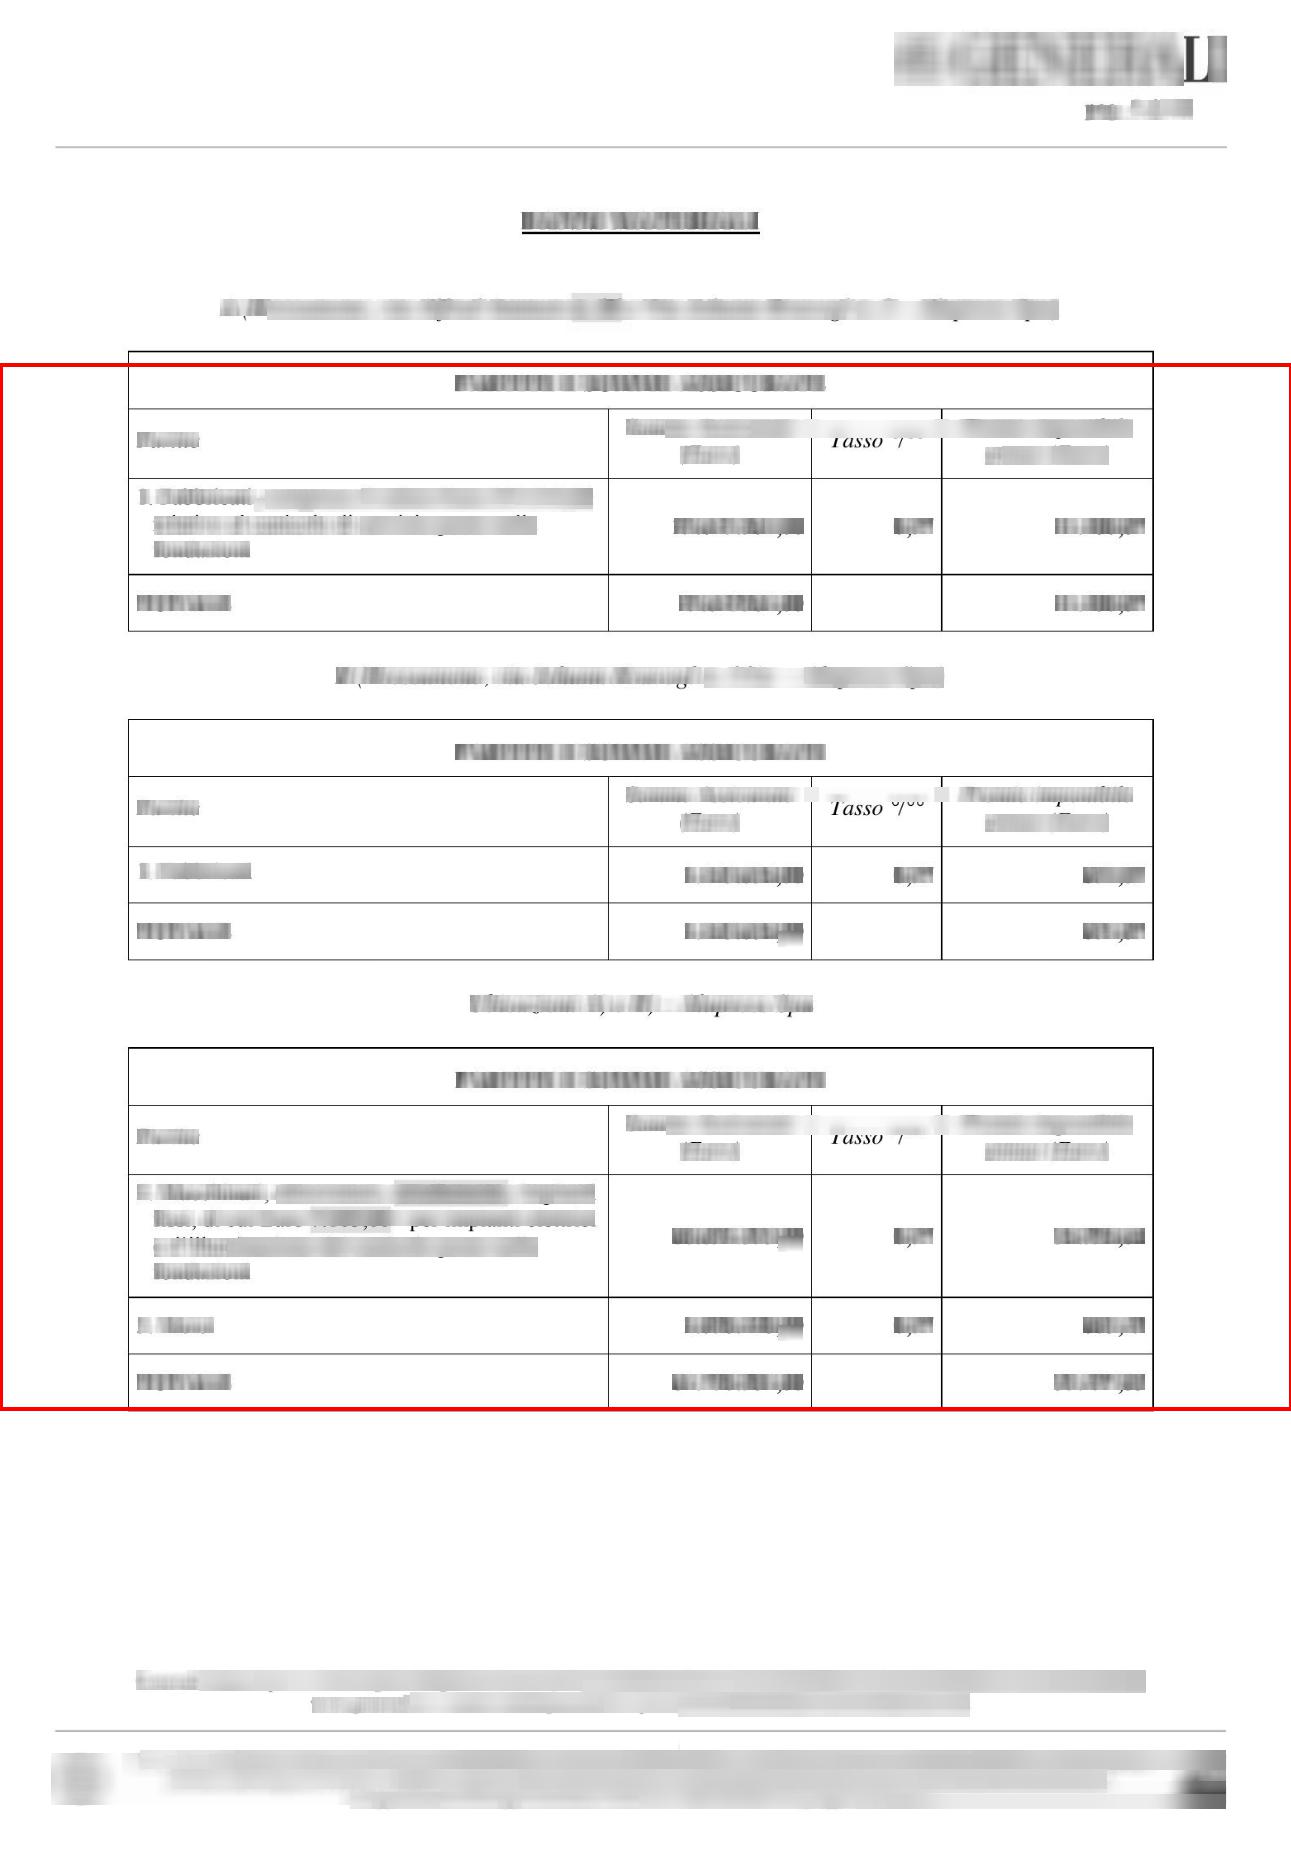
\includegraphics[width=1\columnwidth]{appendice/unite/test1_merged_0_6_momentum_optimizer_1batch}  
    \end{minipage}  
    \caption{Test 1, configurazione 6}
\end{figure}%  
Configurazione:
\begin{multicols}{2}
    \begin{lstlisting}
image_resizer {
  fixes_shape_resizer {
    width: 400
    heigth: 400
  }
}
first_stage_box_predictor {
  l2_regularizer {
    weight: 0.04
}
first_stage_nms_iou_threshold: 0.7
second_stage_box_predictor {
  l2_regularizer {
    weight: 0.004
  }
}
second_stage_post_processing {
  iou_threshold: 0.6
}
batch_size: 1
optimizer {
  adam_optimizer: {
    learning_rate: {
      manual_step_learning_rate {
        initial_learning_rate: 0.0004
        schedule {
          step: 4500
          learning_rate: .0002
        }
        schedule {
          step: 7000
          learning_rate: .00002
        }
        schedule {
          step: 10000
          learning_rate: .000002
        }
    ...
    }
    momentum_optimizer_value: 0.9
  }
  use_moving_average: false
}
    \end{lstlisting}
\end{multicols}
%============================================================================================
\newpage
\subsection{Test 2}
\begin{figure}[!ht] 
    \centering
    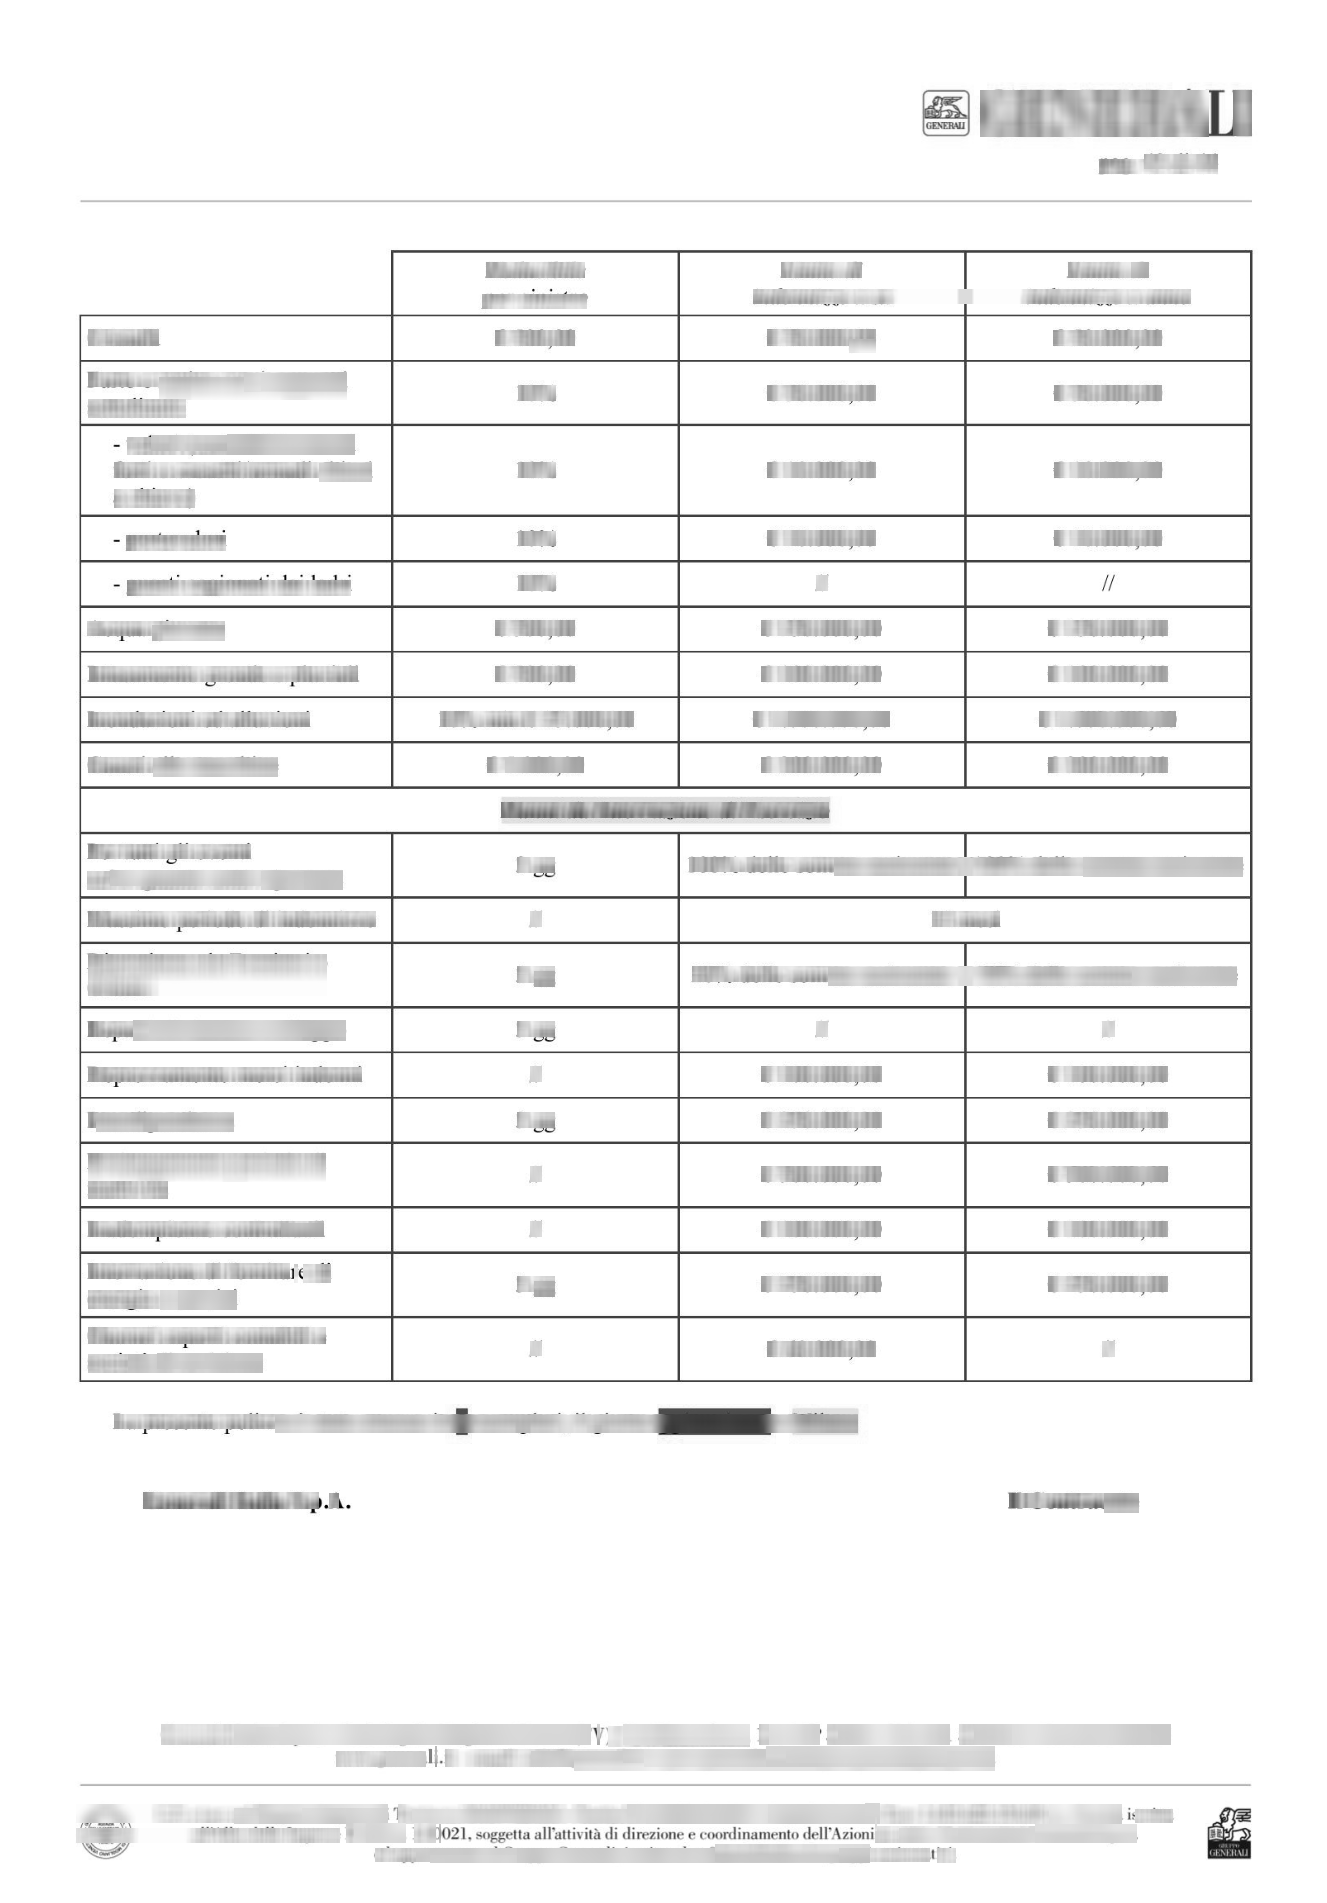
\includegraphics[width=1\columnwidth]{appendice/test2} 
    \caption{Test 2}
    \label{img:test-1}
\end{figure} 
\newpage

%============================================================================================


\begin{figure}[H]  
    \begin{minipage}{.5\columnwidth}  
        \centering  
        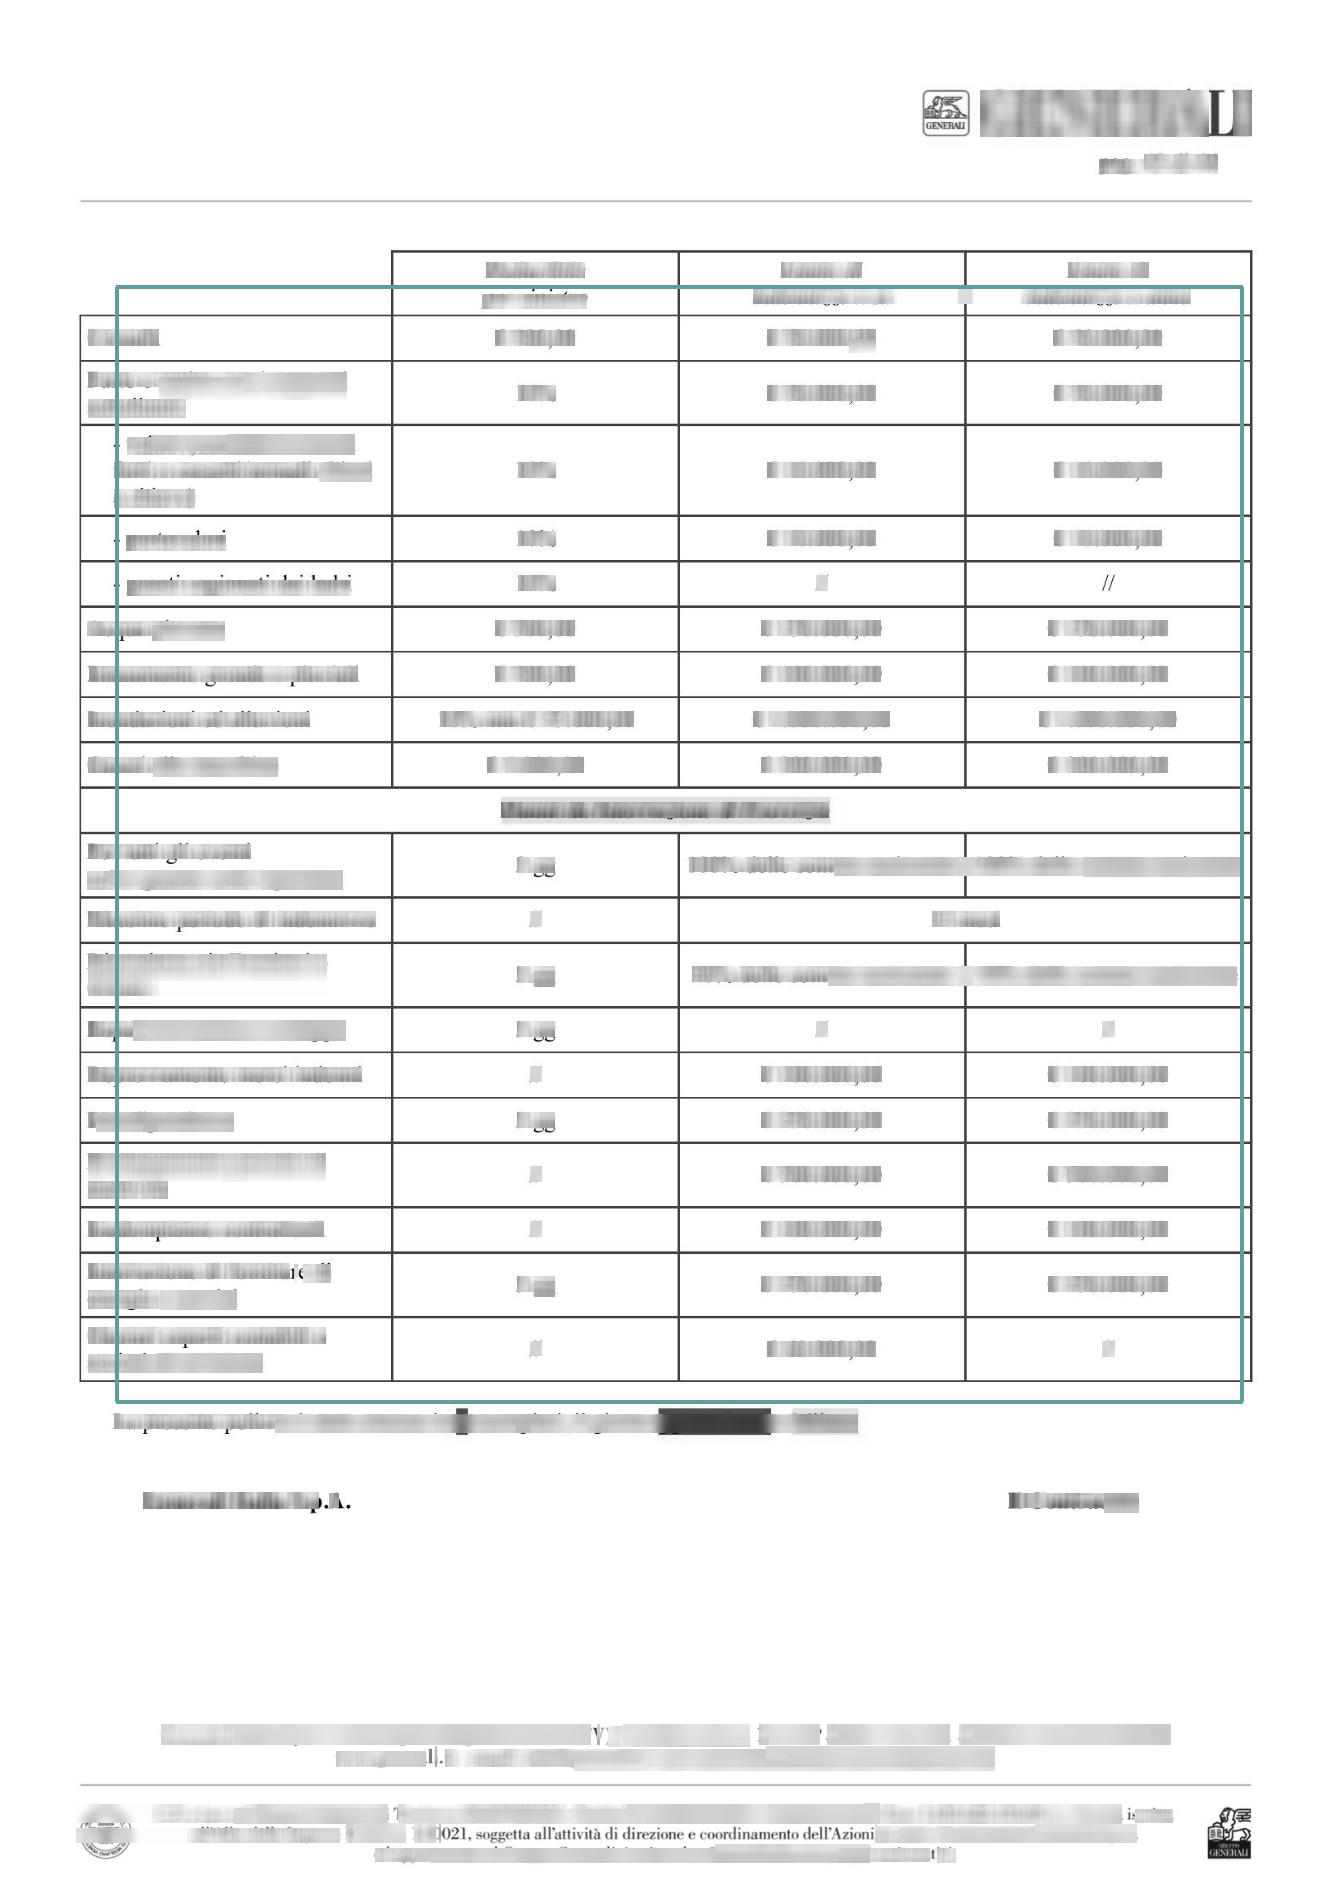
\includegraphics[width=1\columnwidth]{appendice/filtrate/test2_filtered_0_6_adam_1}  
    \end{minipage}%  
    \begin{minipage}{0.5\columnwidth}  
        \centering  
        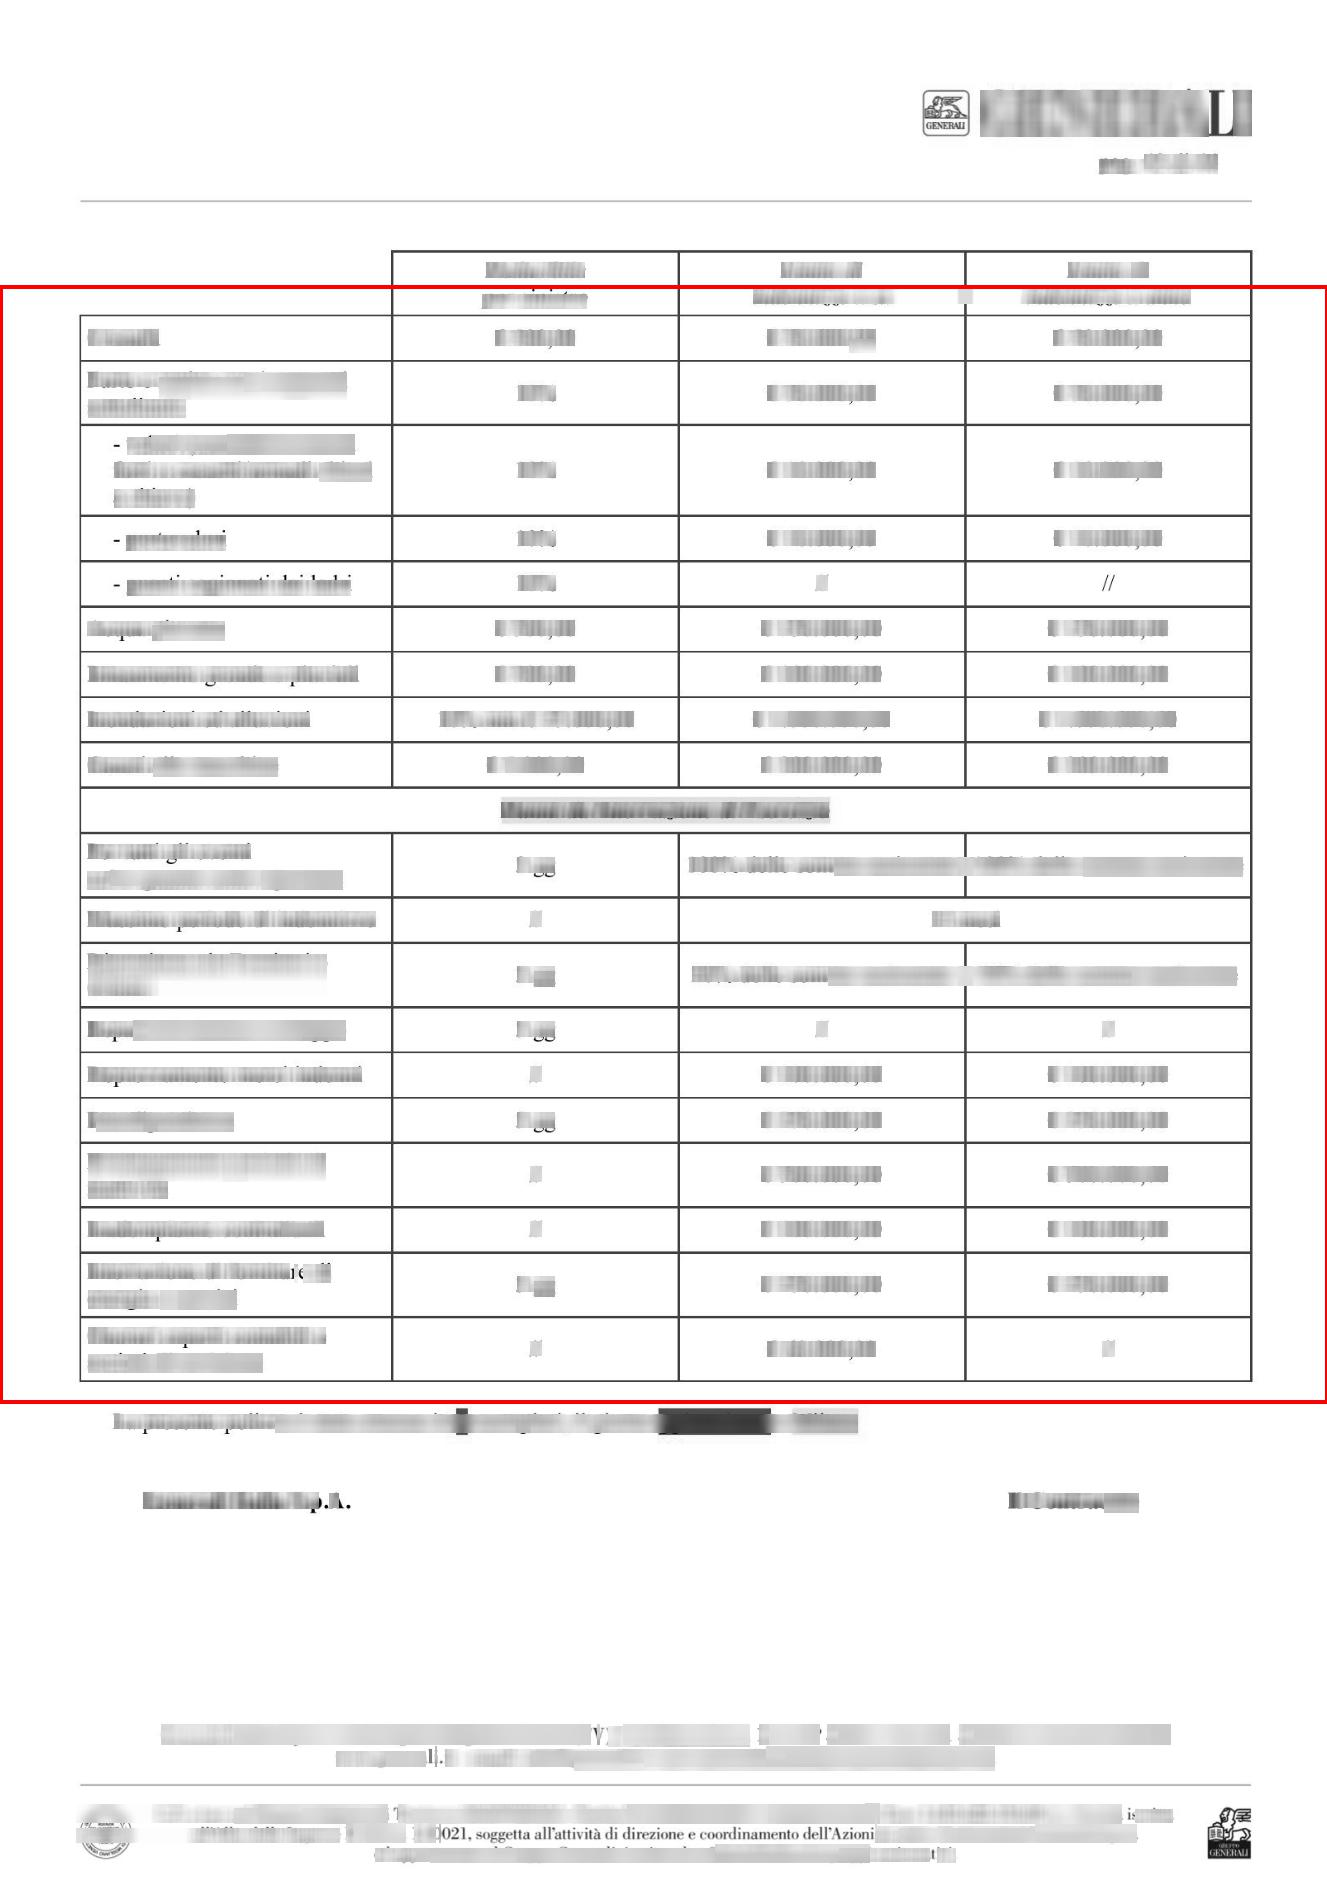
\includegraphics[width=1\columnwidth]{appendice/unite/test2_merged_0_6_adam_1}  
    \end{minipage}  
    \caption{Test 2, configurazione 1}
\end{figure}%  
Configurazione:
\begin{multicols}{2}
    \begin{lstlisting}
image_resizer {
  fixes_shape_resizer {
    width: 400
    heigth: 400
  }
}
first_stage_box_predictor {
  l2_regularizer {
    weight: 0.008
}
first_stage_nms_iou_threshold: 0.7
second_stage_box_predictor {
  l2_regularizer {
    weight: 0.004
  }
}
second_stage_post_processing {
  iou_threshold: 0.6
}
optimizer {
  adam_optimizer: {
    learning_rate: {
      manual_step_learning_rate {
        initial_learning_rate: .00008
        schedule {
          step: 4500
          learning_rate: .00004
        }
        schedule {
          step: 7000
          learning_rate: .00002
        }
        schedule {
          step: 10000
          learning_rate: .000008
        }
    ...
    }
    momentum_optimizer_value: 0.9
  }
  use_moving_average: false
}
\end{lstlisting}
\end{multicols}

%============================================================================================
\newpage
\begin{figure}[H]  
    \begin{minipage}{.5\columnwidth}  
        \centering  
        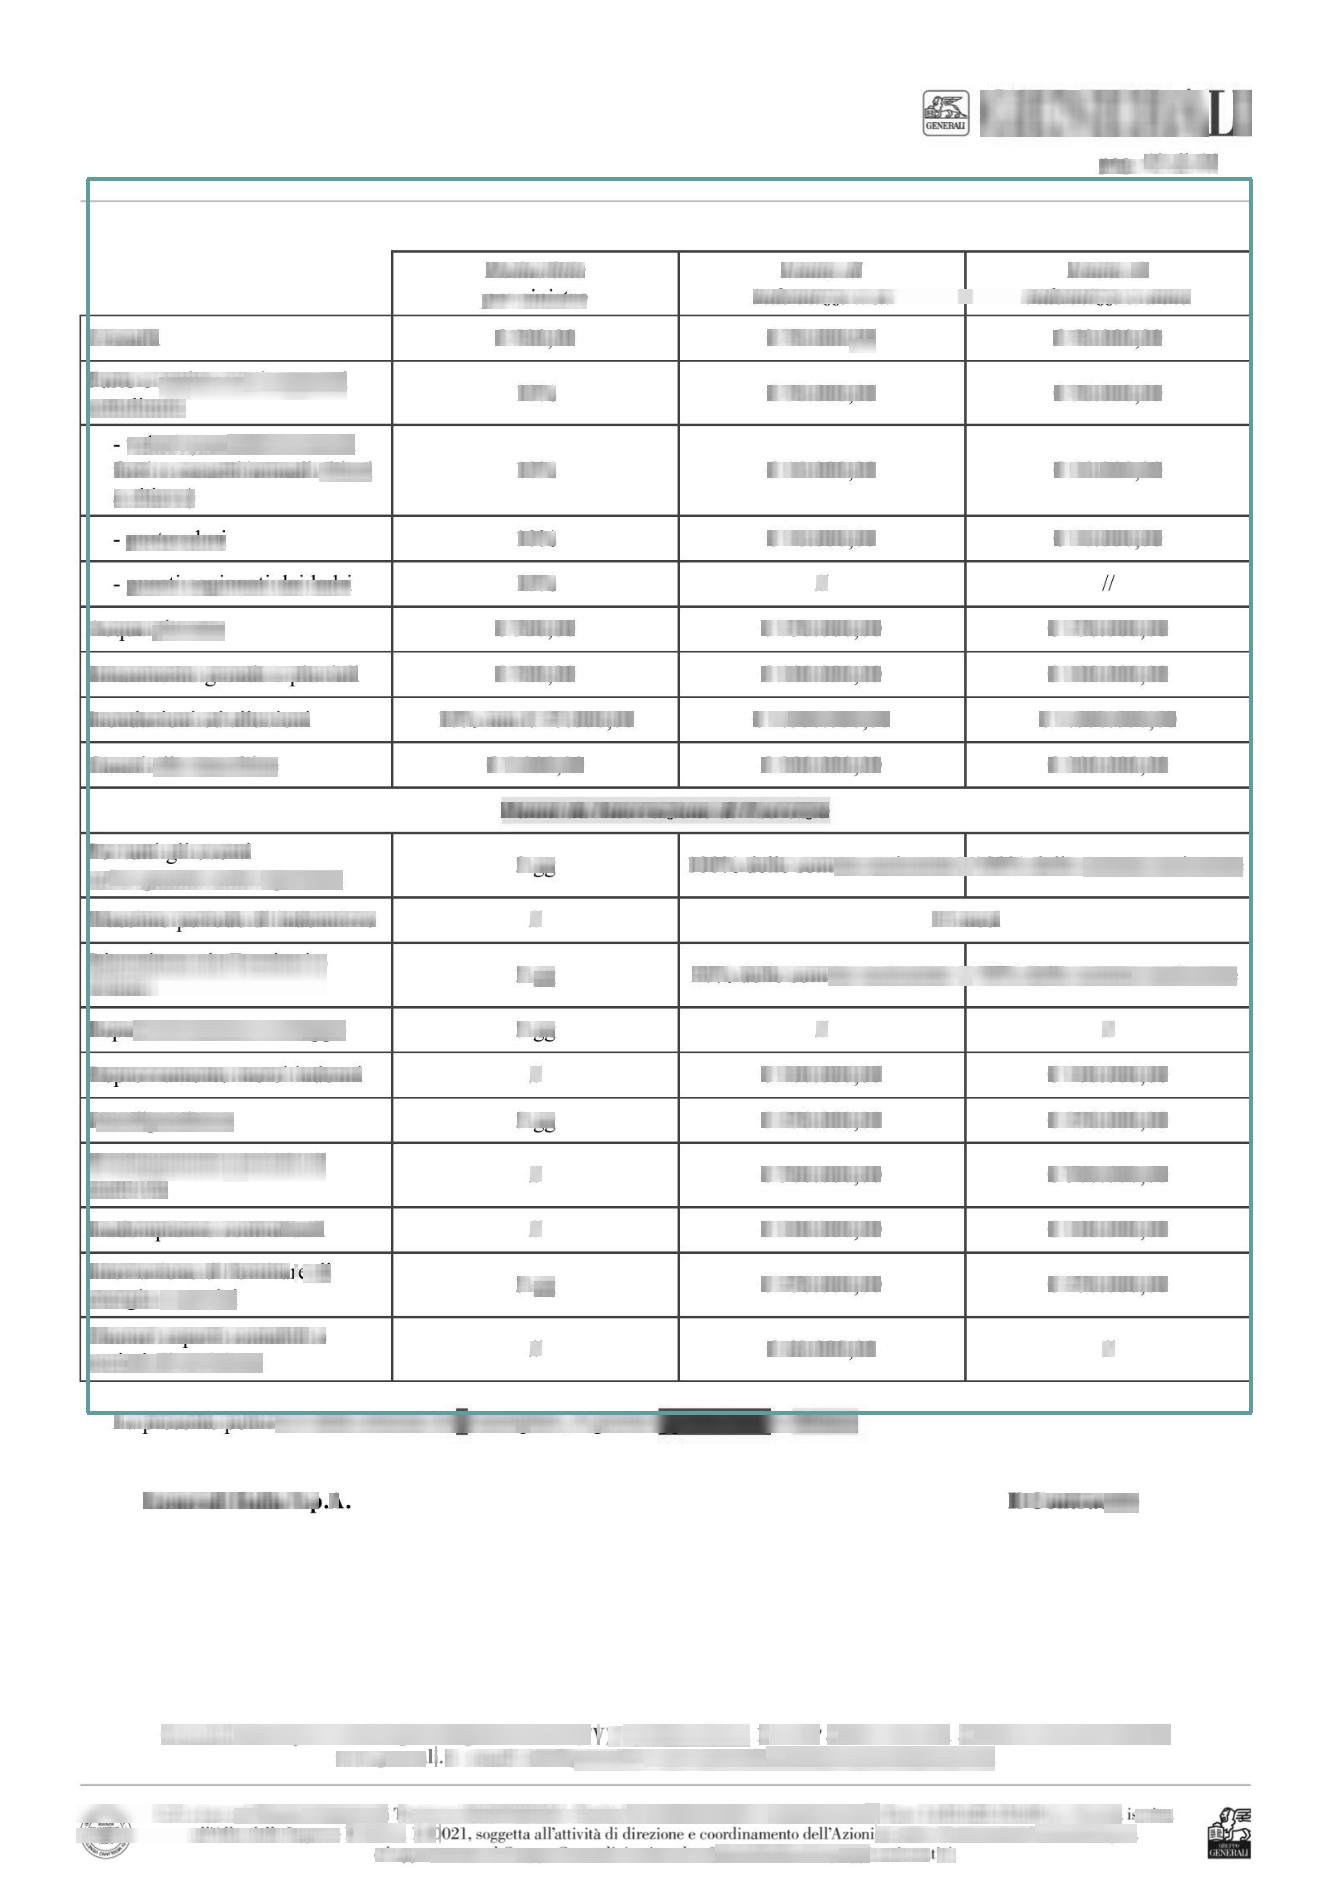
\includegraphics[width=1\columnwidth]{appendice/filtrate/test2_filtered_0_6_adam_3}  
    \end{minipage}%  
    \begin{minipage}{0.5\columnwidth}  
        \centering  
        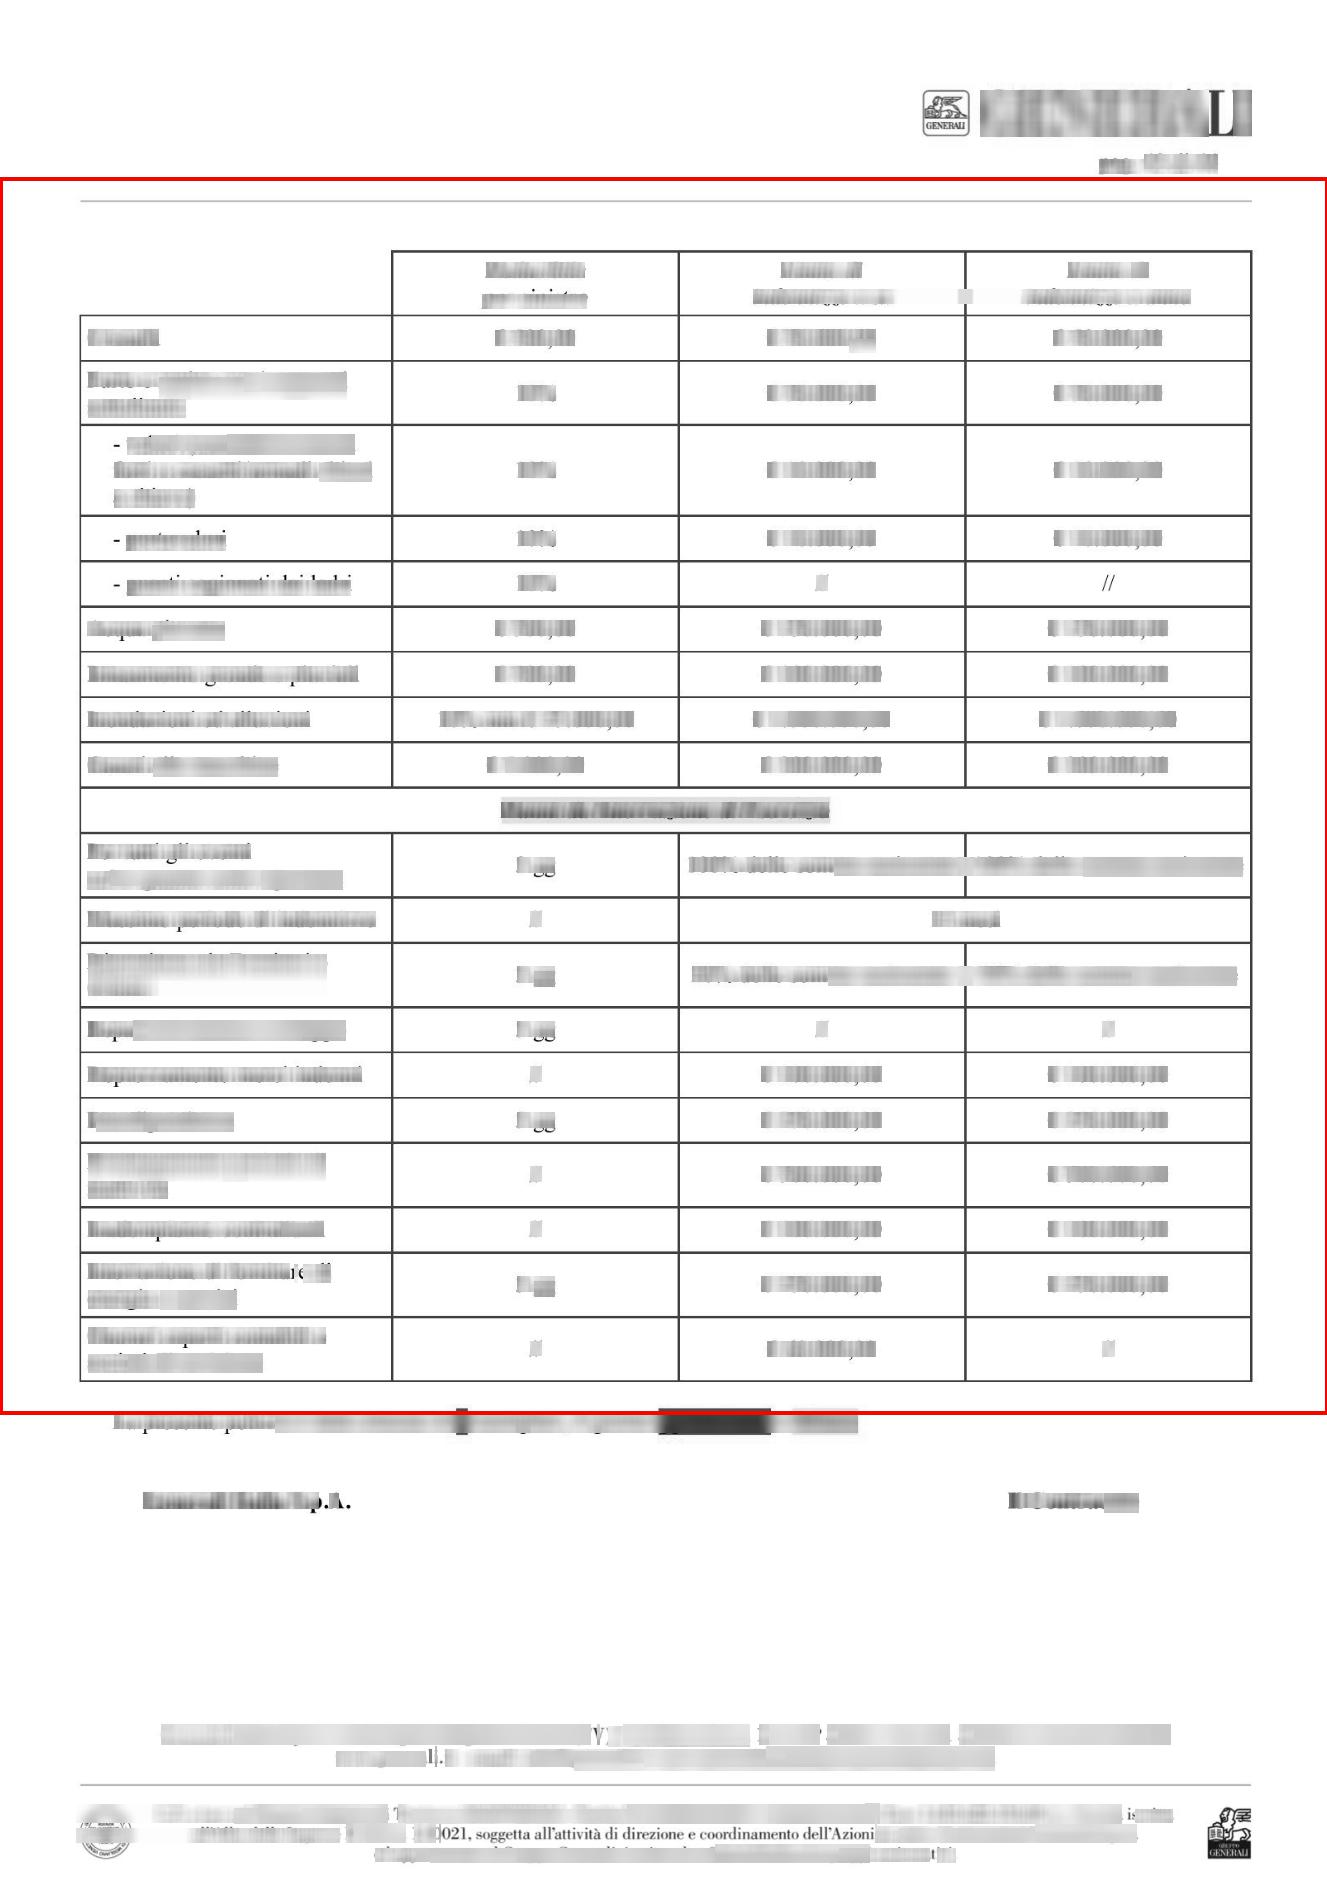
\includegraphics[width=1\columnwidth]{appendice/unite/test2_merged_0_6_adam_3}  
    \end{minipage}  
    \caption{Test 2, configurazione 2}
\end{figure}%  
Configurazione:
\begin{multicols}{2}
    \begin{lstlisting}
image_resizer {
  fixes_shape_resizer {
    width: 400
    heigth: 400
  }
}
first_stage_box_predictor {
  l2_regularizer {
    weight: 0.00001
}
first_stage_nms_iou_threshold: 0.7
second_stage_box_predictor {
  l2_regularizer {
    weight: 0.00004
  }
}
second_stage_post_processing {
  iou_threshold: 0.6
}
optimizer {
  adam_optimizer: {
    learning_rate: {
      exponential_decay_learning_rate {
        initial_learning_rate: 0.0001
          decay_steps: 600
          decay_factor: 0.95
        }
      }
    ...
  use_moving_average: false
}
    \end{lstlisting}
\end{multicols}

%============================================================================================
\newpage
\begin{figure}[H]  
    \begin{minipage}{.5\columnwidth}  
        \centering  
        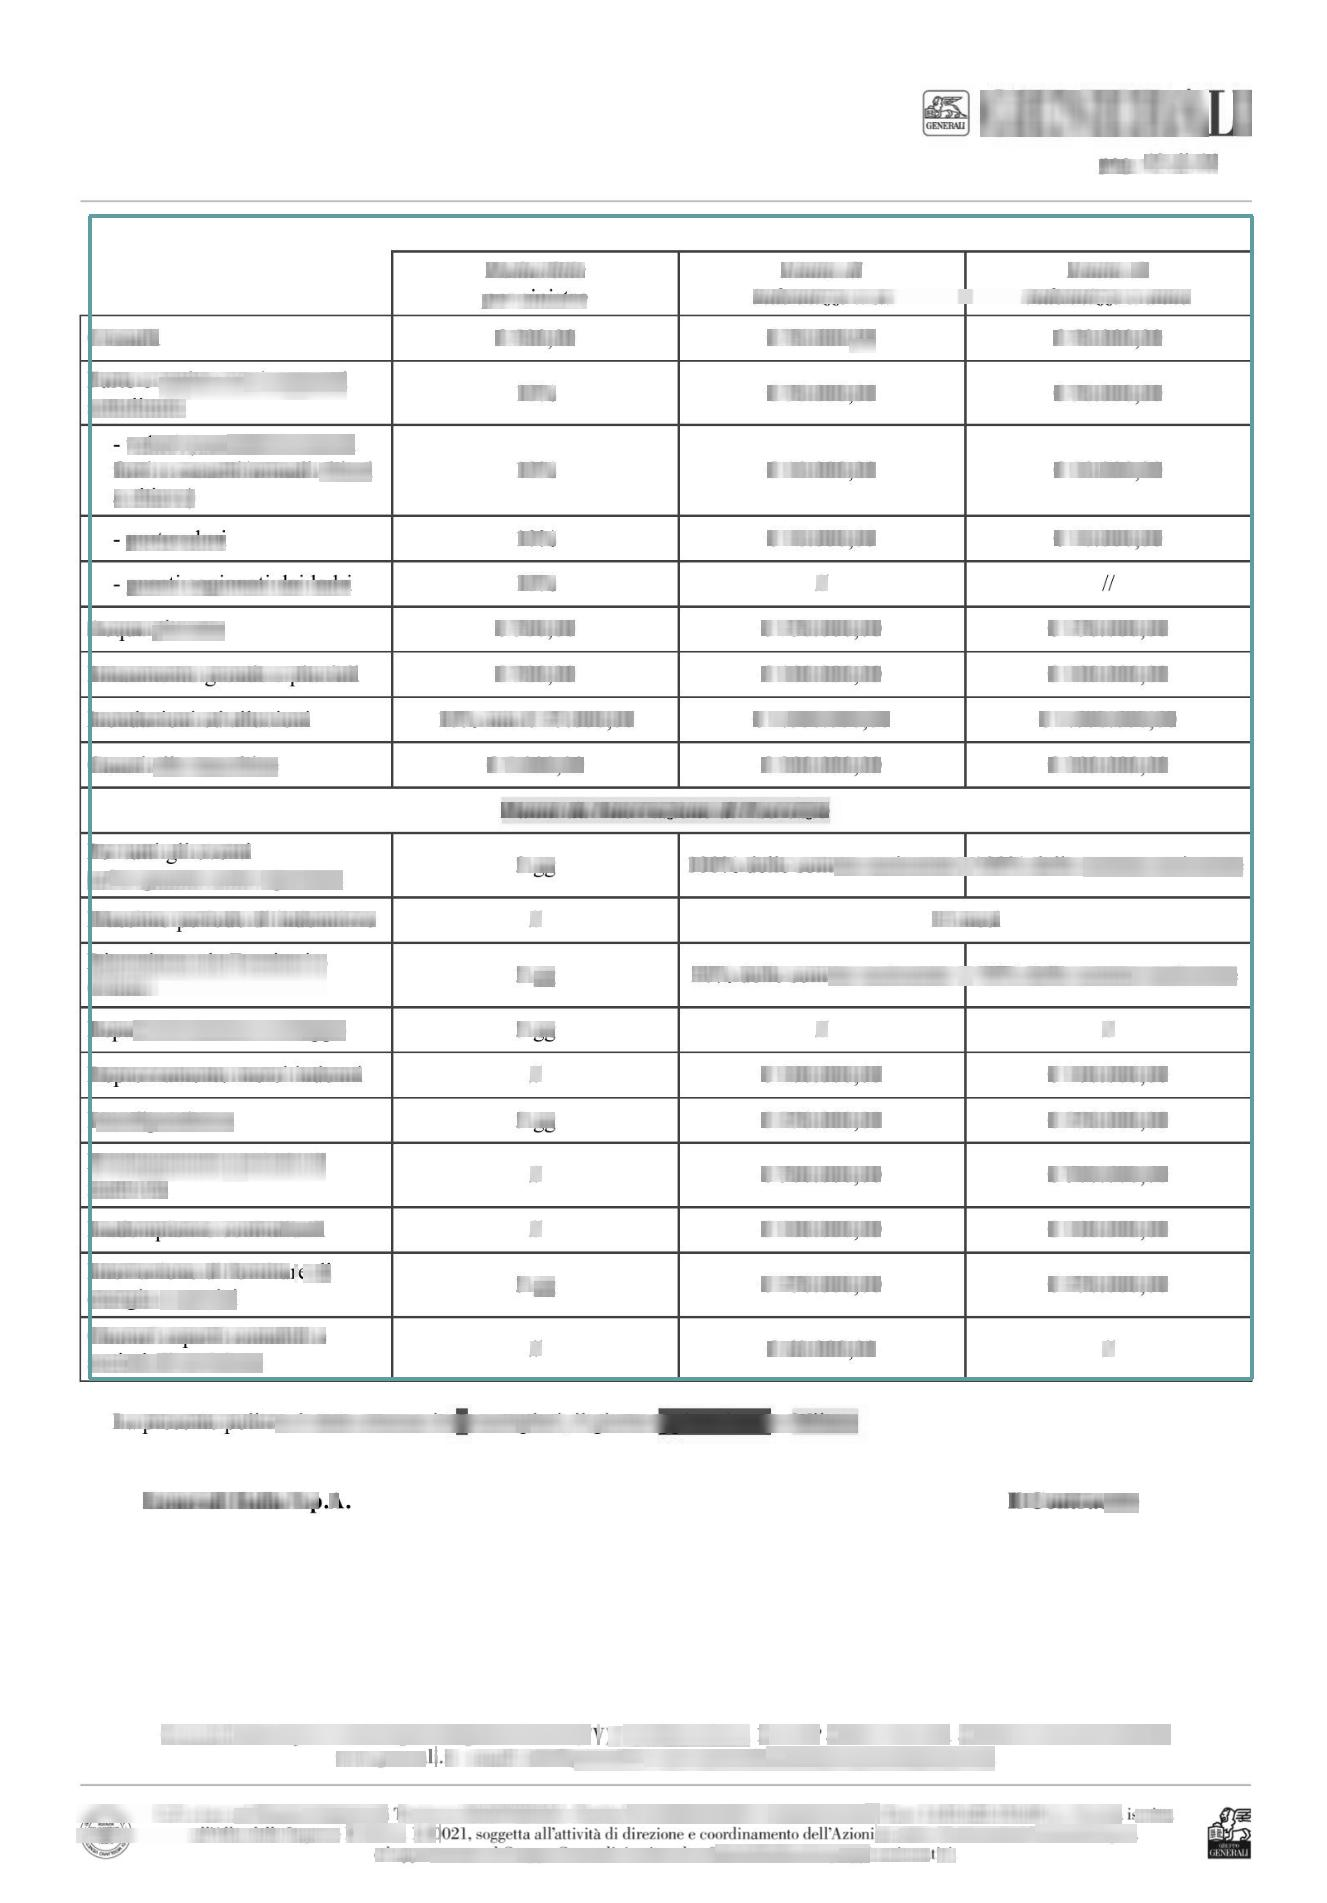
\includegraphics[width=1\columnwidth]{appendice/filtrate/test2_filtered_0_6_adam_4}  
    \end{minipage}%  
    \begin{minipage}{0.5\columnwidth}  
        \centering  
        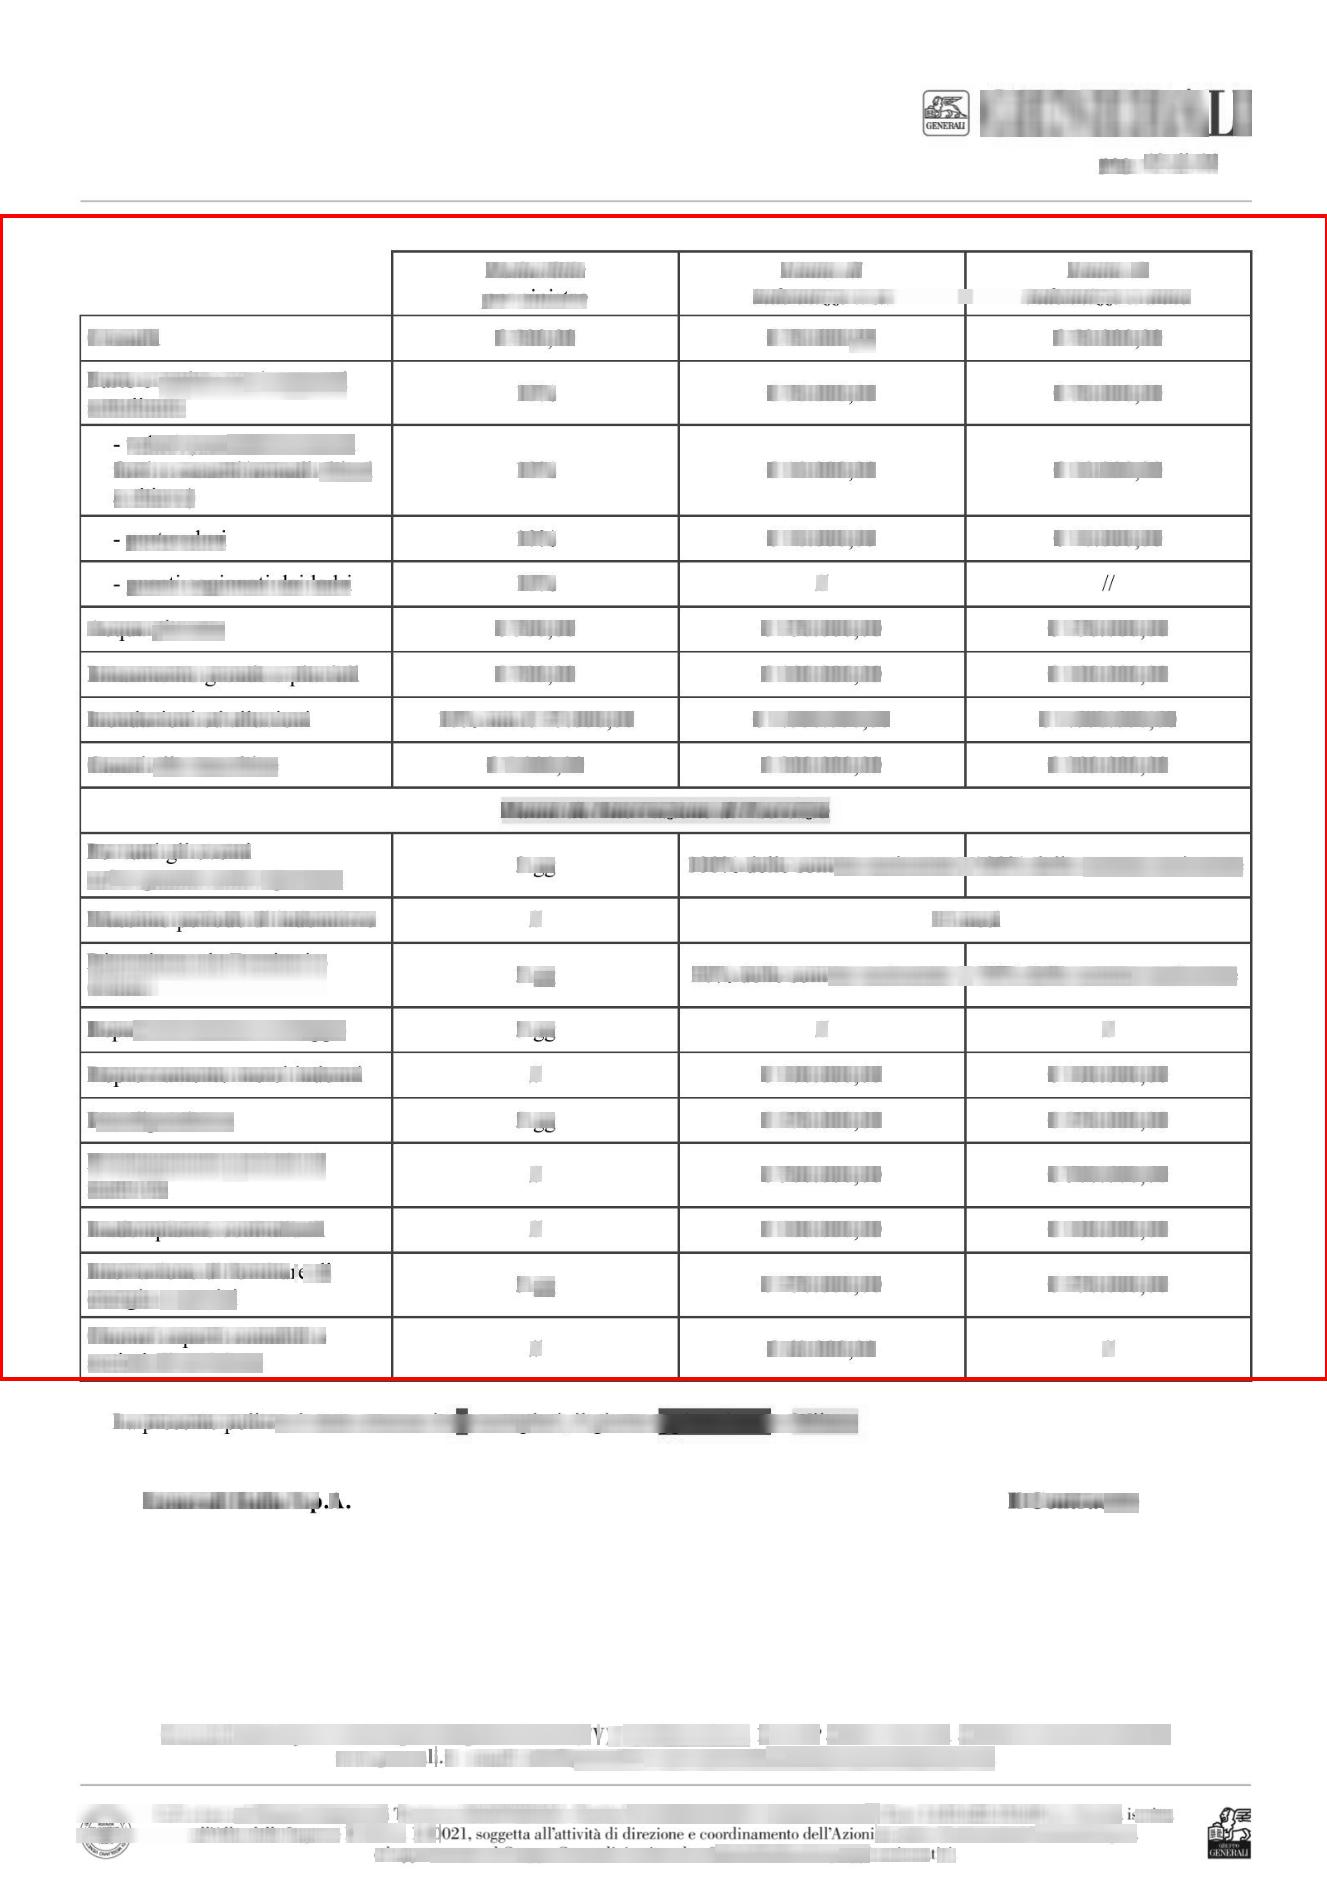
\includegraphics[width=1\columnwidth]{appendice/unite/test2_merged_0_6_adam_4}  
    \end{minipage}  
    \caption{Test 2, configurazione 3}
\end{figure}%  
Configurazione:
\begin{multicols}{2}
    \begin{lstlisting}
image_resizer {
  fixes_shape_resizer {
    width: 400
    heigth: 400
  }
}
first_stage_box_predictor {
  l2_regularizer {
    weight: 0.04
}
first_stage_nms_iou_threshold: 0.7
second_stage_box_predictor {
  l2_regularizer {
    weight: 0.004
  }
}
second_stage_post_processing {
  iou_threshold: 0.6
}
optimizer {
  adam_optimizer: {
    learning_rate: {
      exponential_decay_learning_rate {
        initial_learning_rate: 0.0001
          decay_steps: 450
          decay_factor: 0.9
        }
      }
    ...
  use_moving_average: false
}
    \end{lstlisting}
\end{multicols}

%============================================================================================
\newpage
\begin{figure}[H]  
    \begin{minipage}{.5\columnwidth}  
        \centering  
        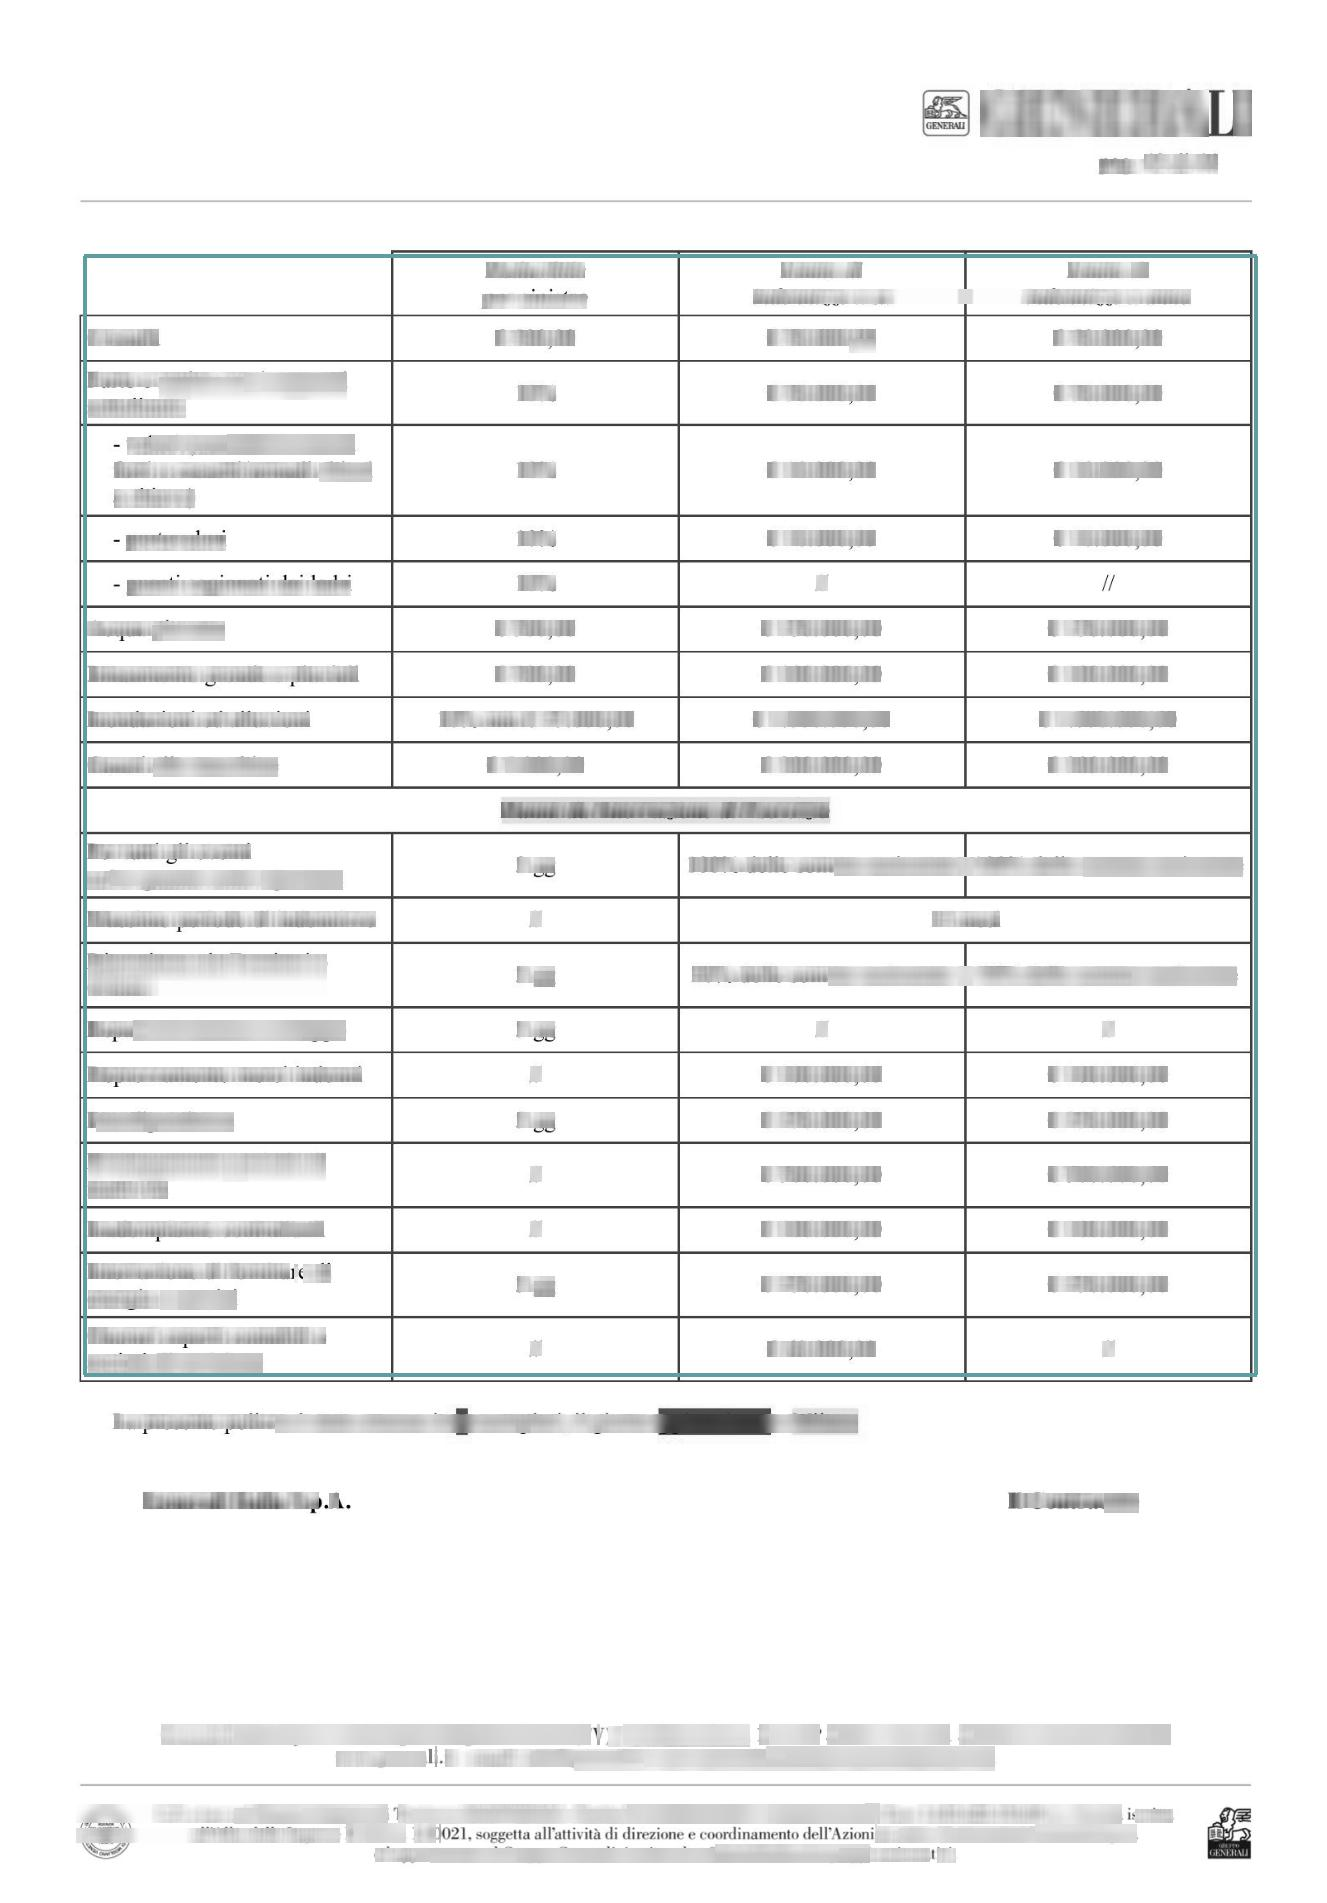
\includegraphics[width=1\columnwidth]{appendice/filtrate/test2_filtered_0_6_momentum_1}  
    \end{minipage}%  
    \begin{minipage}{0.5\columnwidth}  
        \centering  
        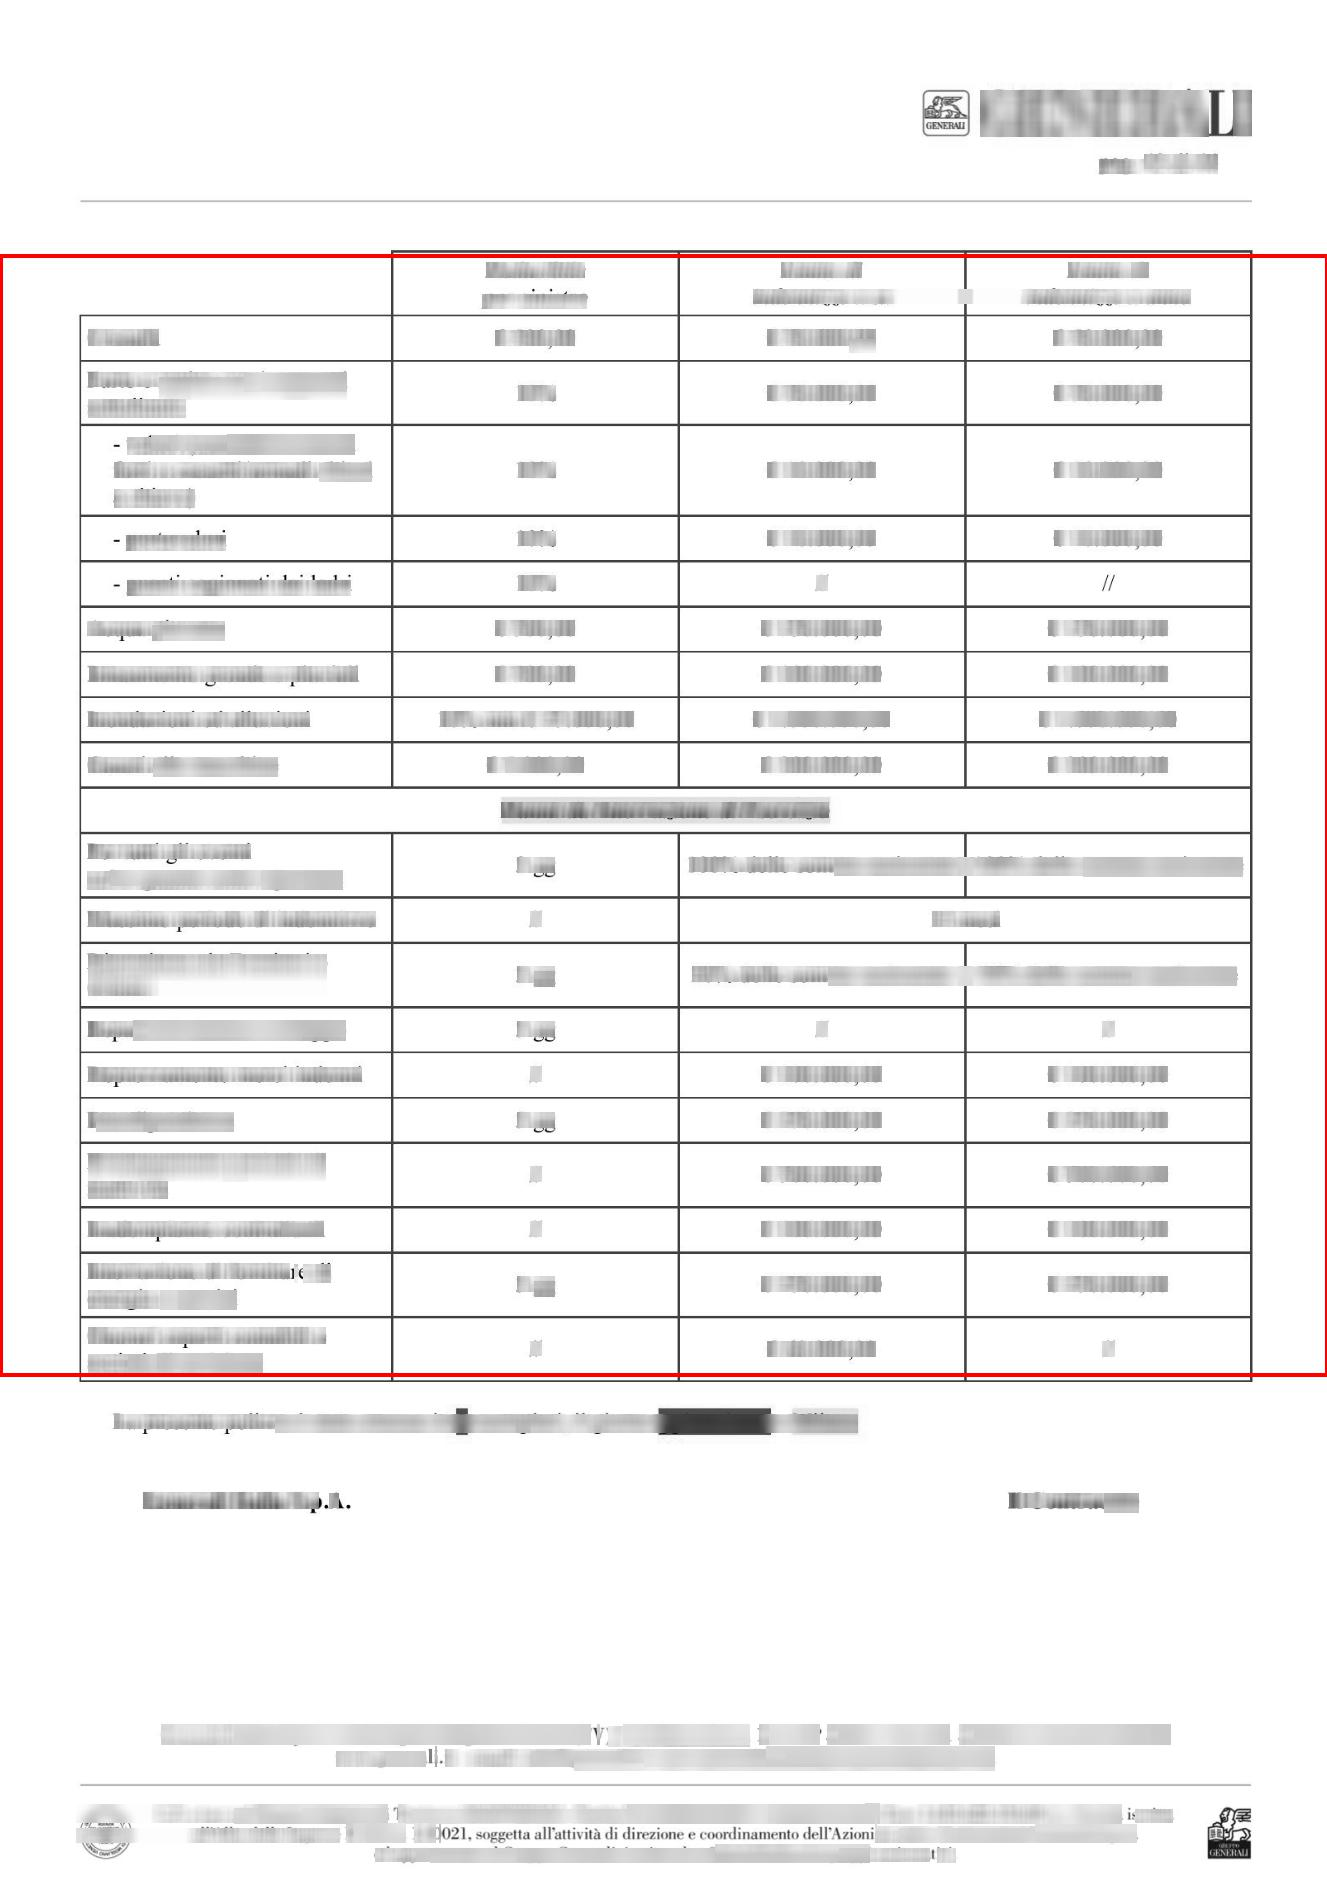
\includegraphics[width=1\columnwidth]{appendice/unite/test2_merged_0_6_momentum_1}  
    \end{minipage}  
    \caption{Test 2, configurazione 4}
\end{figure}%  
Configurazione:
\begin{multicols}{2}
    \begin{lstlisting}
image_resizer {
  fixes_shape_resizer {
    width: 400
    heigth: 400
  }
}
first_stage_box_predictor {
  l2_regularizer {
    weight: 0.00001
}
first_stage_nms_iou_threshold: 0.7
second_stage_box_predictor {
  l2_regularizer {
    weight: 0.00004
  }
}
second_stage_post_processing {
  iou_threshold: 0.6
}
optimizer {
  adam_optimizer: {
    learning_rate: {
      manual_step_learning_rate {
        initial_learning_rate: 0.0008
        schedule {
          step: 4500
          learning_rate: .0008
        }
        schedule {
          step: 7000
          learning_rate: .0004
        }
        schedule {
          step: 10000
          learning_rate: .00008
        }
    ...
    }
    momentum_optimizer_value: 0.9
  }
  use_moving_average: false
}
    \end{lstlisting}
\end{multicols}
%============================================================================================

\newpage
\begin{figure}[H]  
    \begin{minipage}{.5\columnwidth}  
        \centering  
        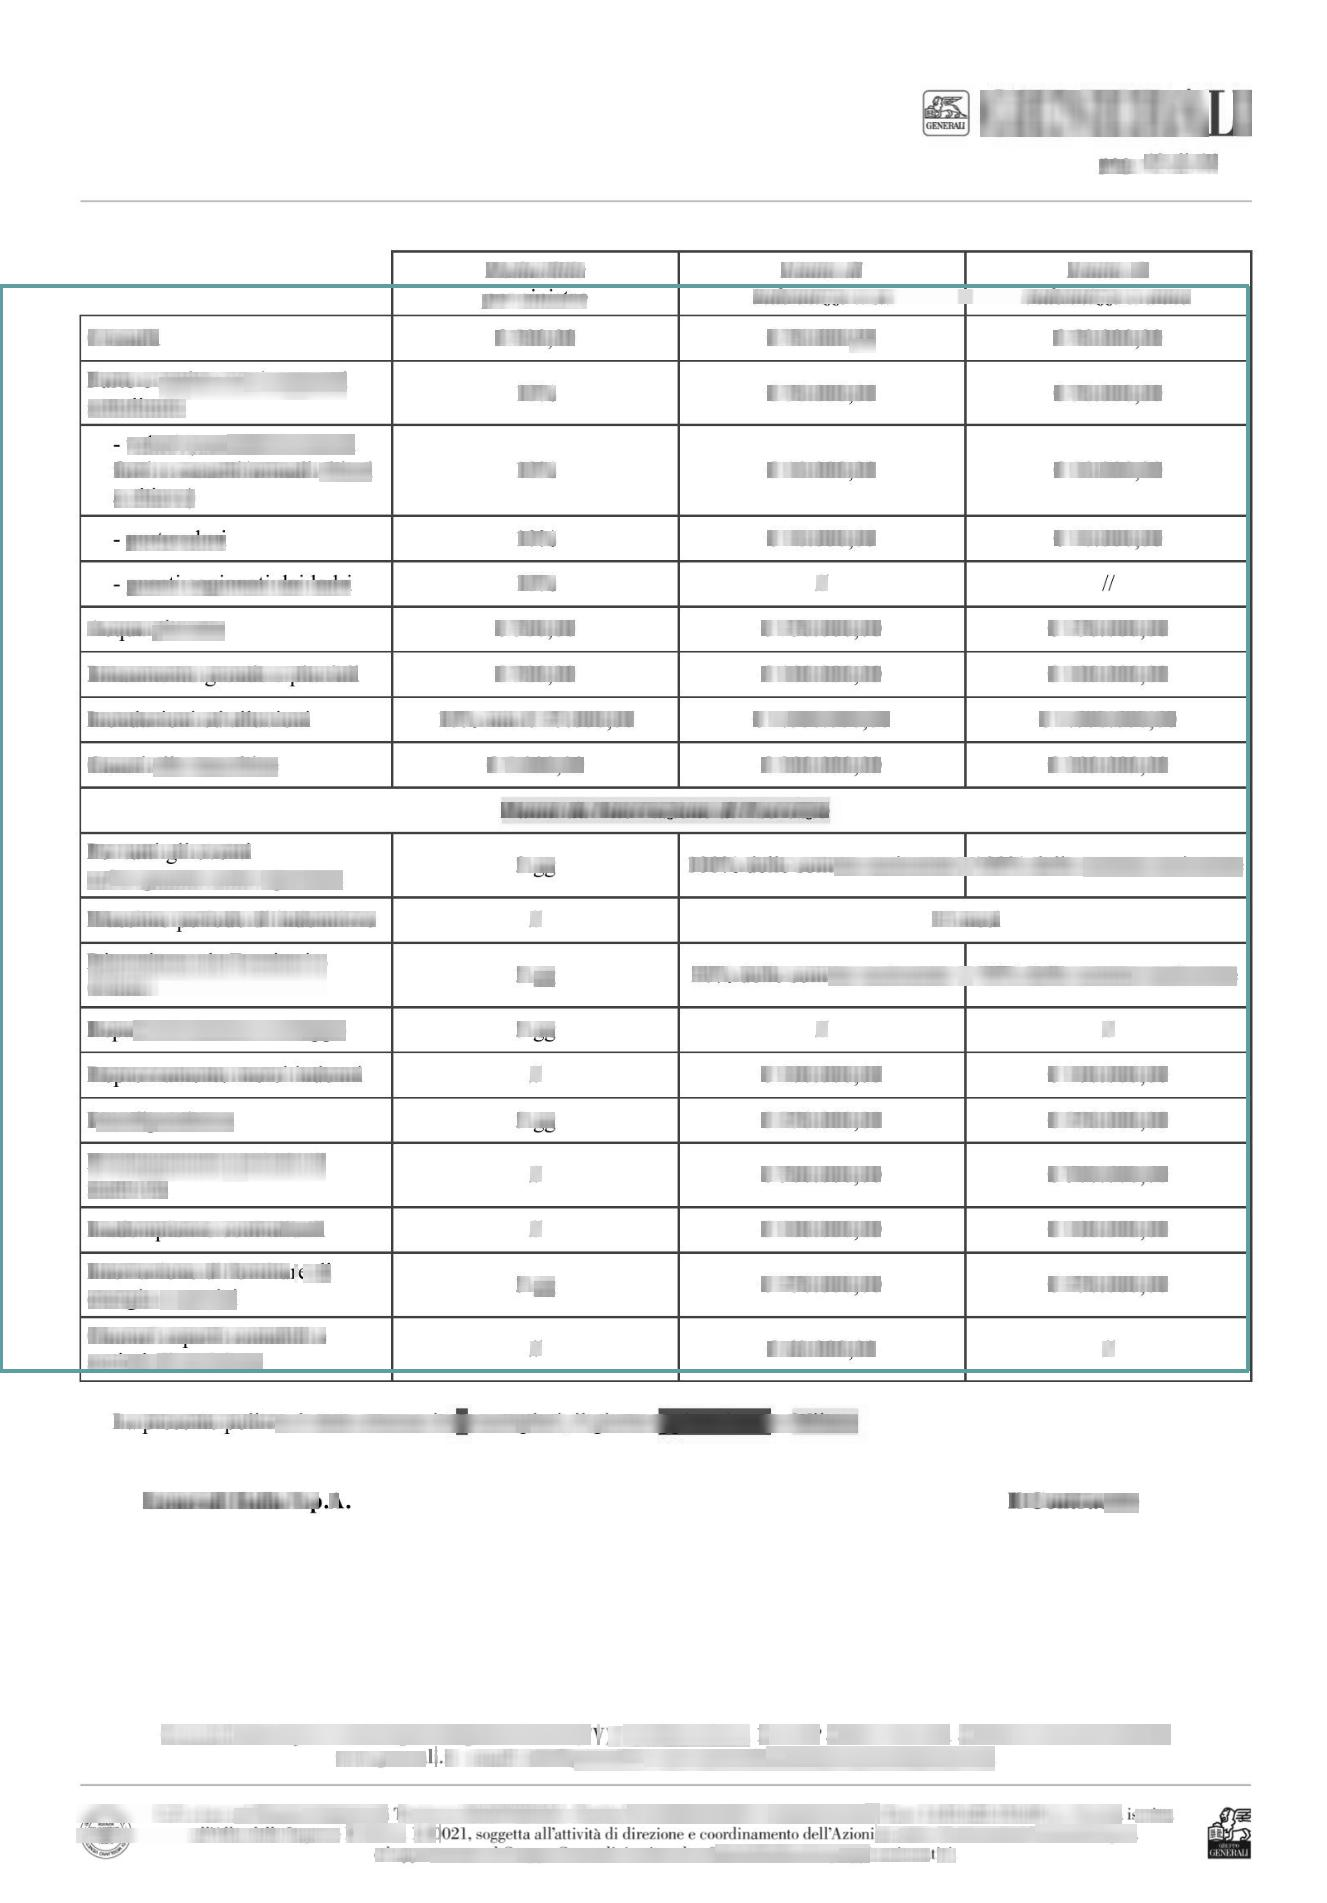
\includegraphics[width=1\columnwidth]{appendice/filtrate/test2_filtered_0_6_momentum_10k_jpg}  
    \end{minipage}%  
    \begin{minipage}{0.5\columnwidth}  
        \centering  
        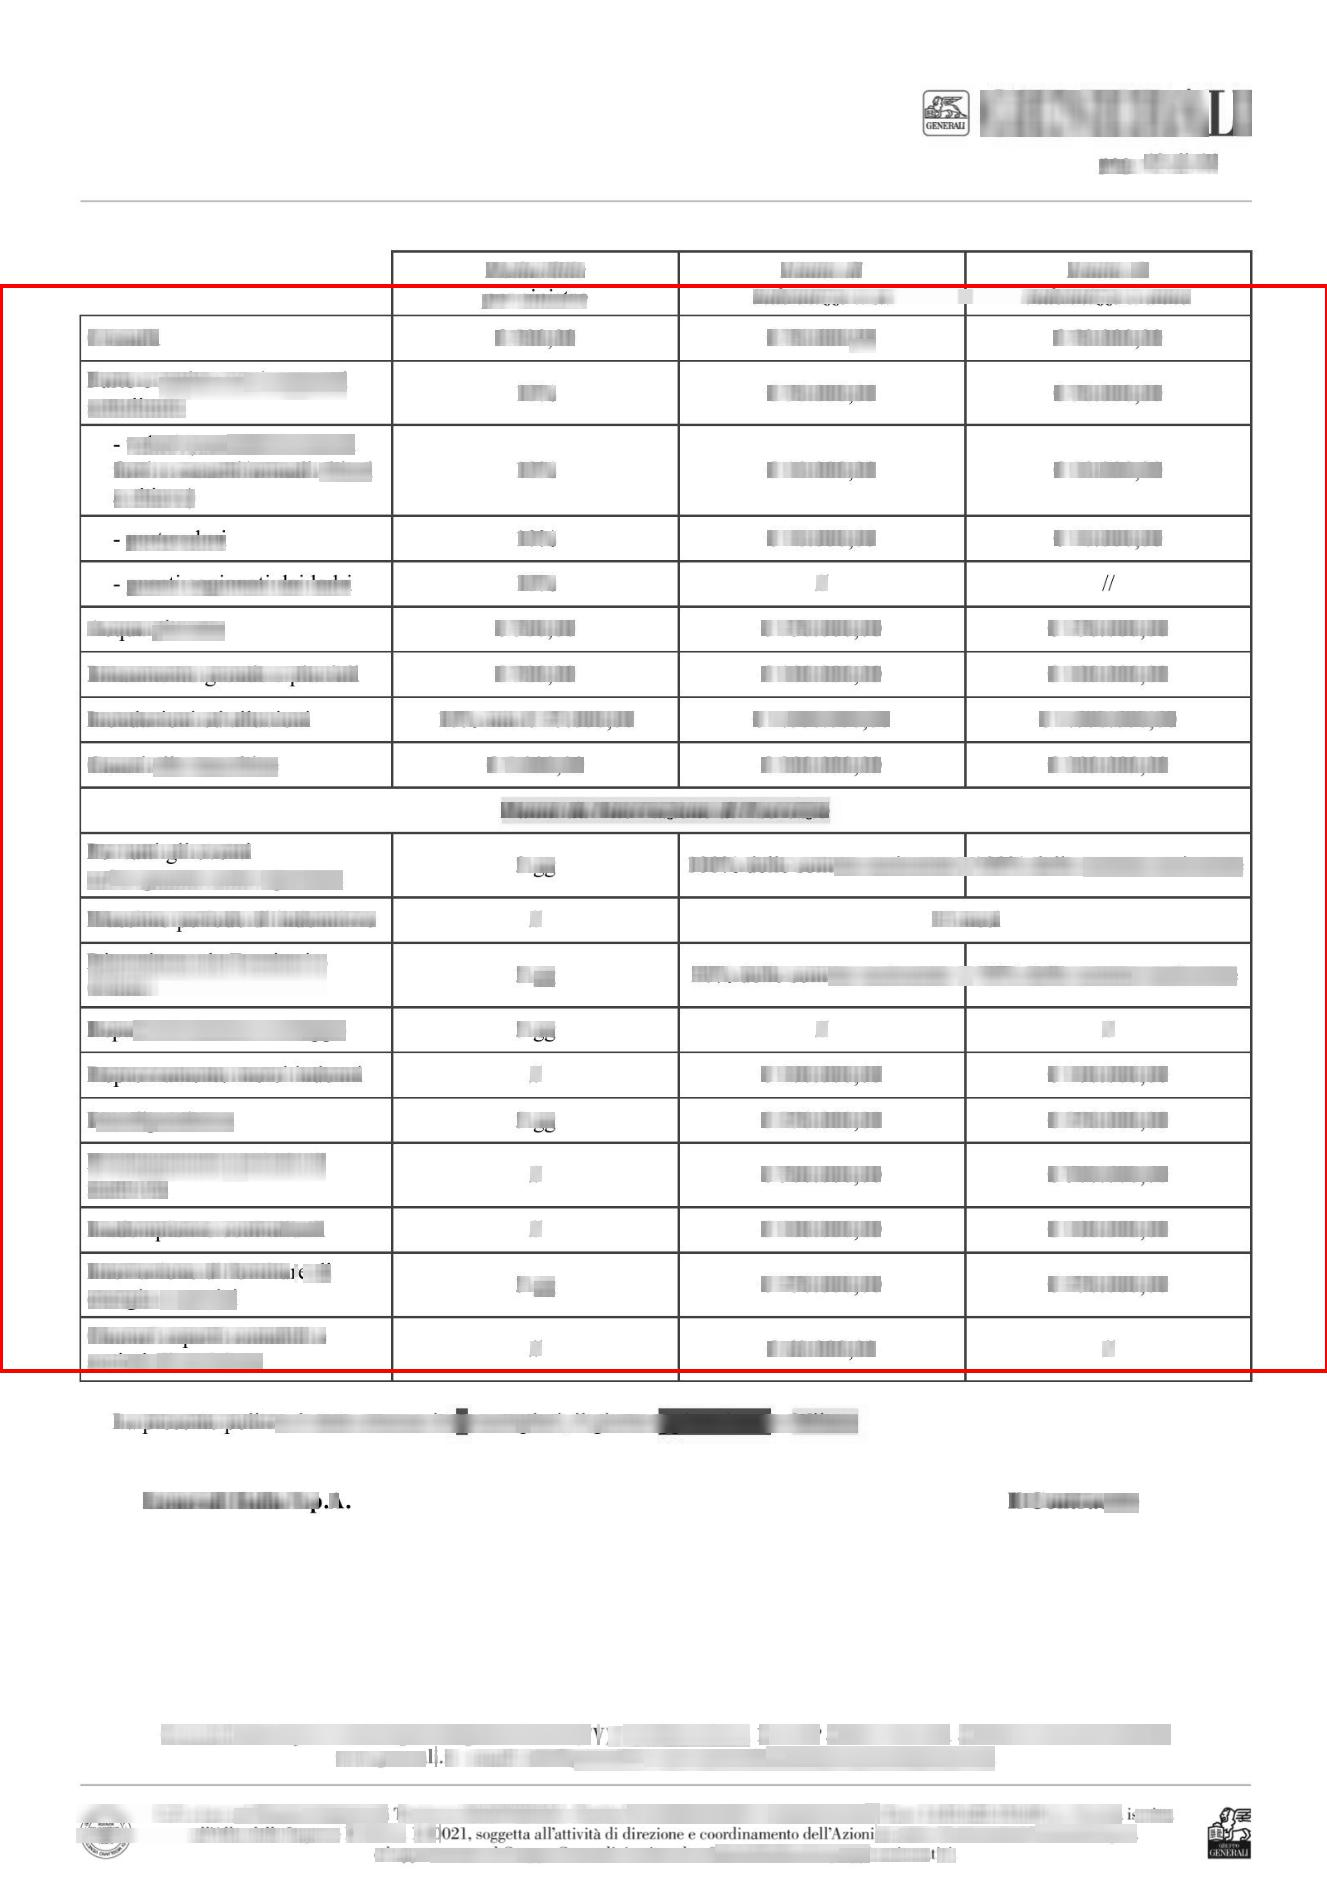
\includegraphics[width=1\columnwidth]{appendice/unite/test2_merged_0_6_momentum_10k_jpg}  
    \end{minipage}  
    \caption{Test 2, configurazione 5}
\end{figure}%  
Configurazione:
\begin{multicols}{2}
    \begin{lstlisting}
image_resizer {
  fixes_shape_resizer {
    width: 400
    heigth: 400
  }
}
first_stage_box_predictor {
  l2_regularizer {
    weight: 0.004
}
first_stage_nms_iou_threshold: 0.7
second_stage_box_predictor {
  l2_regularizer {
    weight: 0.004
  }
}
second_stage_post_processing {
  iou_threshold: 0.6
}
optimizer {
  adam_optimizer: {
    learning_rate: {
      manual_step_learning_rate {
        initial_learning_rate: 0.0004
        schedule {
          step: 4500
          learning_rate: .0002
        }
        schedule {
          step: 7000
          learning_rate: .00002
        }
        schedule {
          step: 10000
          learning_rate: .000002
        }
    ...
    }
    momentum_optimizer_value: 0.9
  }
  use_moving_average: false
}
    \end{lstlisting}
\end{multicols}
%============================================================================================

\newpage
\begin{figure}[H]  
    \begin{minipage}{.5\columnwidth}  
        \centering  
        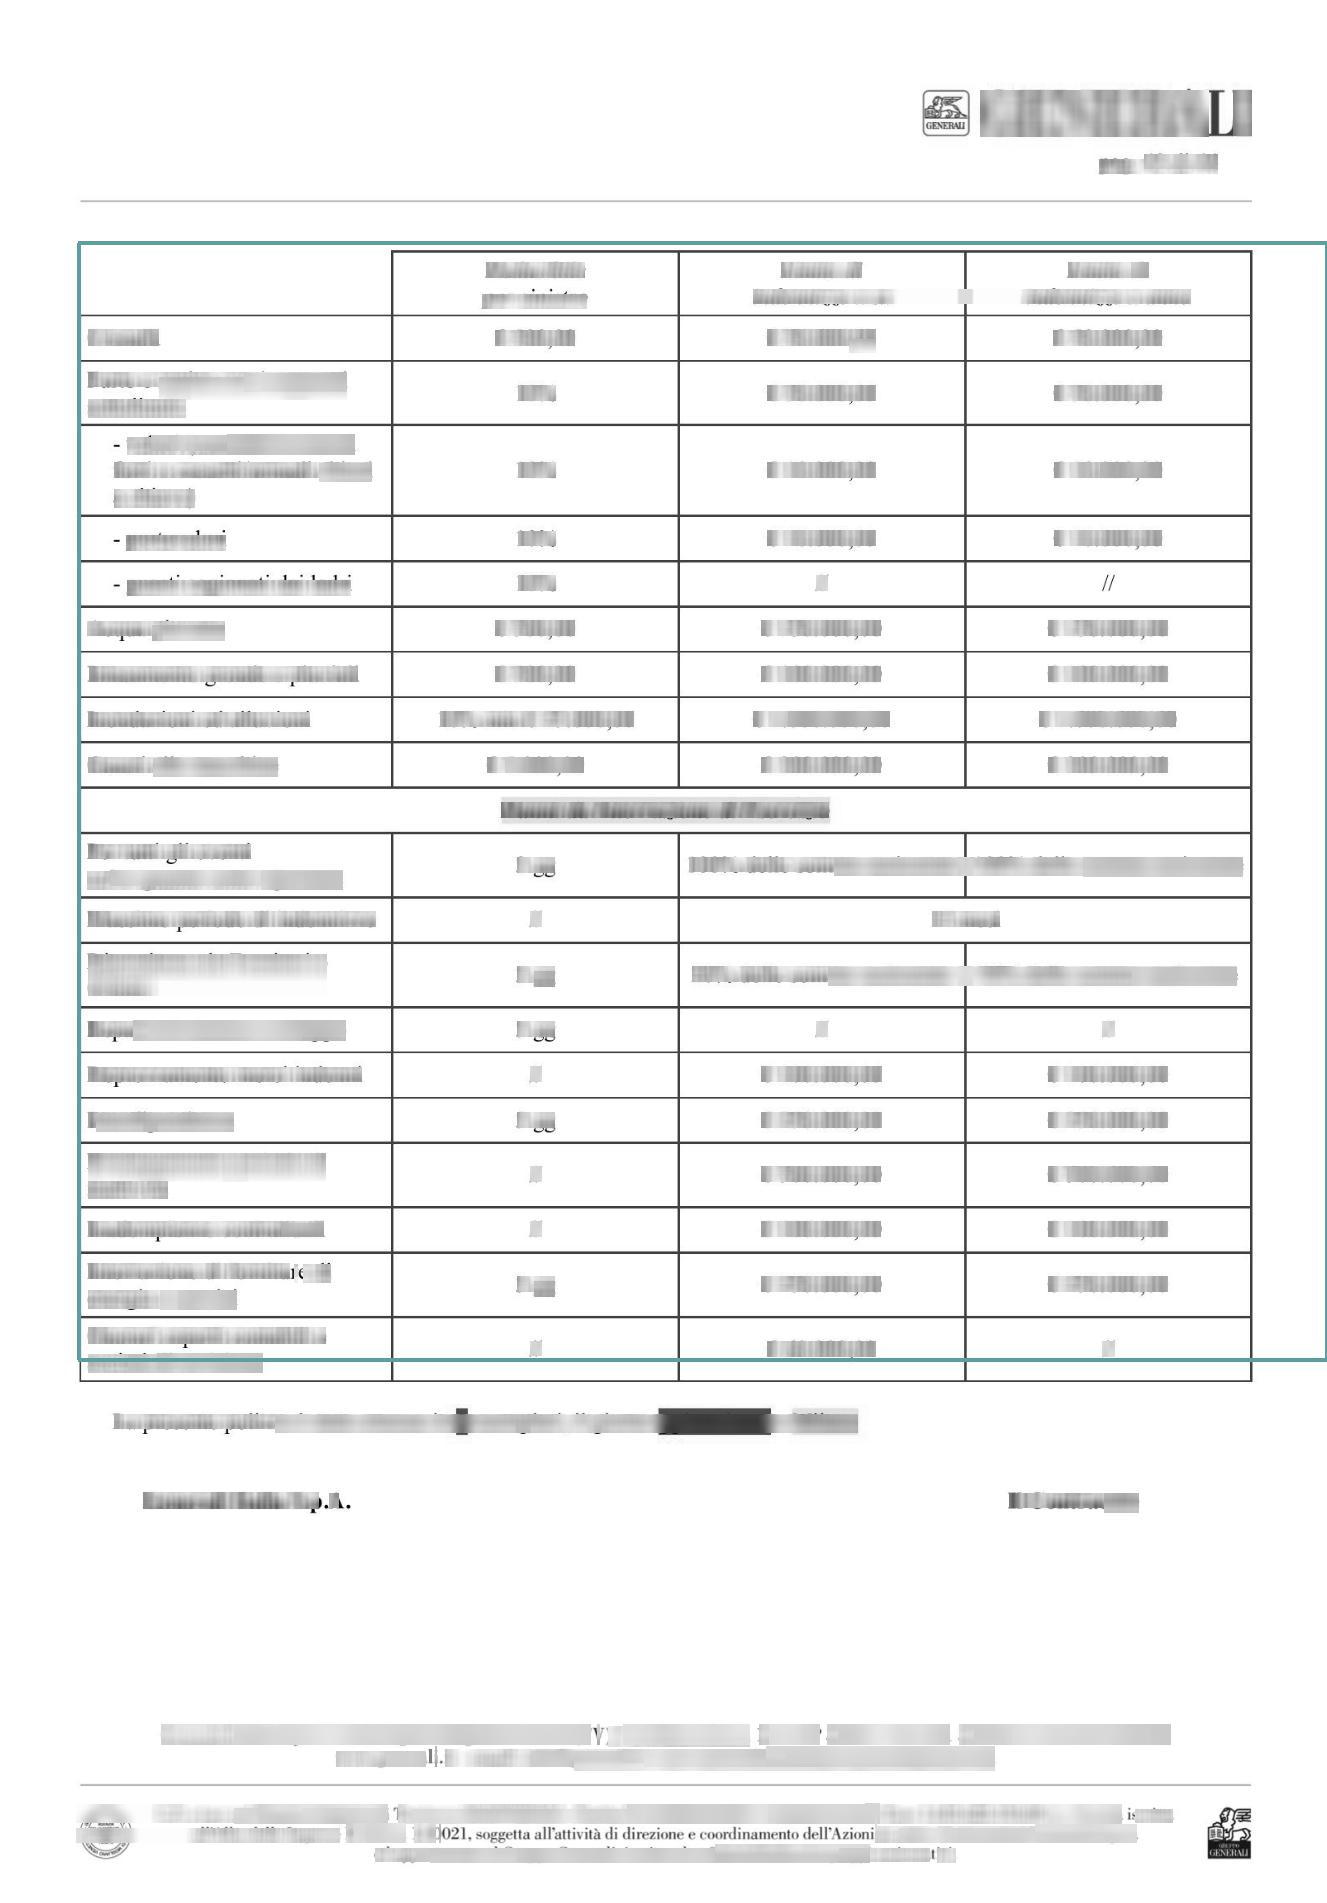
\includegraphics[width=1\columnwidth]{appendice/filtrate/test2_filtered_0_6_momentum_optimizer_1batch}  
    \end{minipage}%  
    \begin{minipage}{0.5\columnwidth}  
        \centering  
        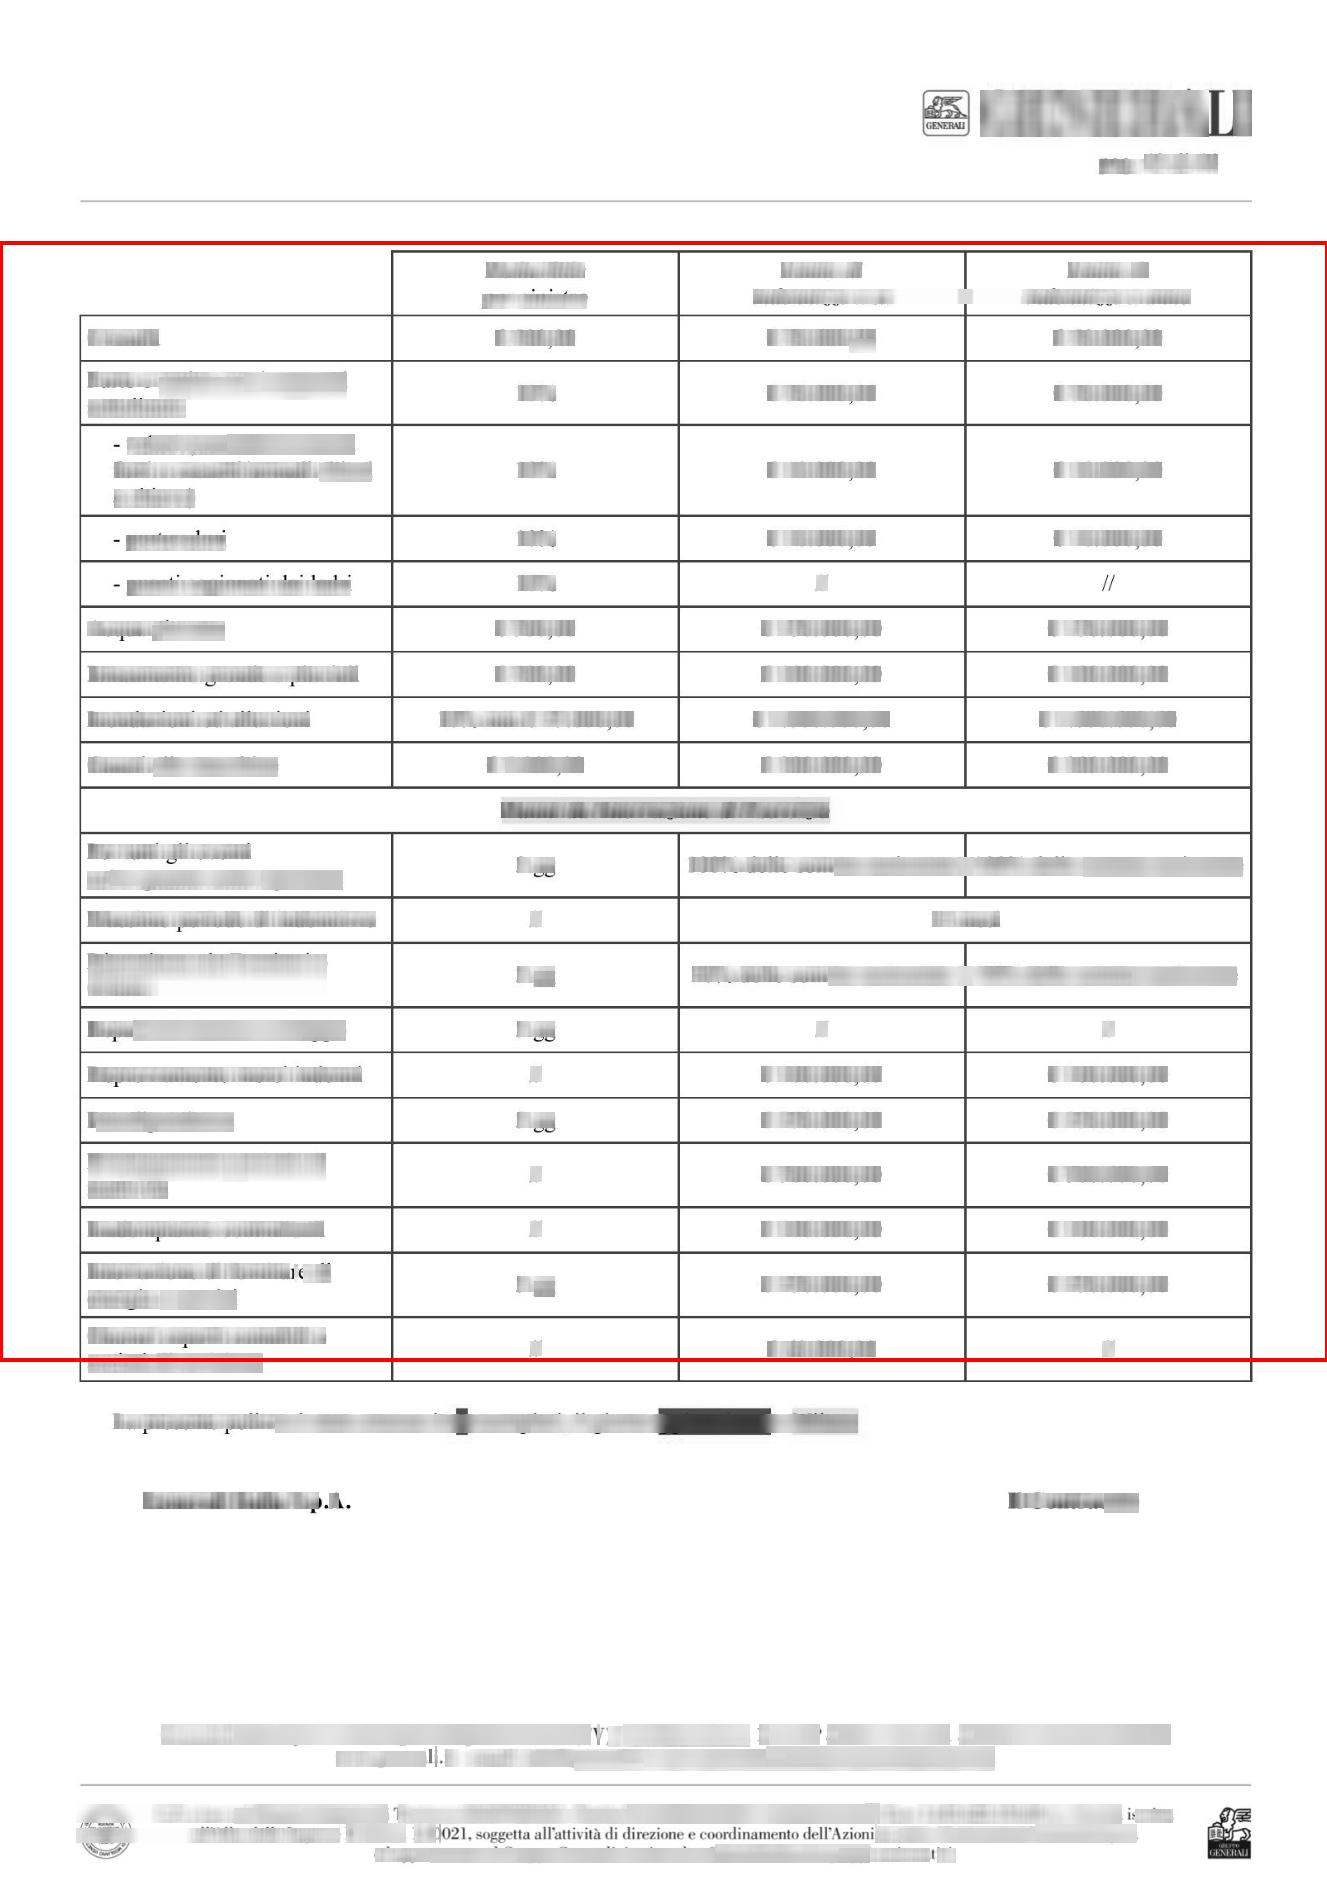
\includegraphics[width=1\columnwidth]{appendice/unite/test2_merged_0_6_momentum_optimizer_1batch}  
    \end{minipage}  
    \caption{Test 2, configurazione 6}
\end{figure}%  
Configurazione:
\begin{multicols}{2}
    \begin{lstlisting}
image_resizer {
  fixes_shape_resizer {
    width: 400
    heigth: 400
  }
}
first_stage_box_predictor {
  l2_regularizer {
    weight: 0.04
}
first_stage_nms_iou_threshold: 0.7
second_stage_box_predictor {
  l2_regularizer {
    weight: 0.004
  }
}
second_stage_post_processing {
  iou_threshold: 0.6
}
batch_size: 1
optimizer {
  adam_optimizer: {
    learning_rate: {
      manual_step_learning_rate {
        initial_learning_rate: 0.0004
        schedule {
          step: 4500
          learning_rate: .0002
        }
        schedule {
          step: 7000
          learning_rate: .00002
        }
        schedule {
          step: 10000
          learning_rate: .000002
        }
    ...
    }
    momentum_optimizer_value: 0.9
  }
  use_moving_average: false
}
    \end{lstlisting}
\end{multicols}
%============================================================================================
\newpage
\subsection{Test 3}
\begin{figure}[!ht] 
    \centering
    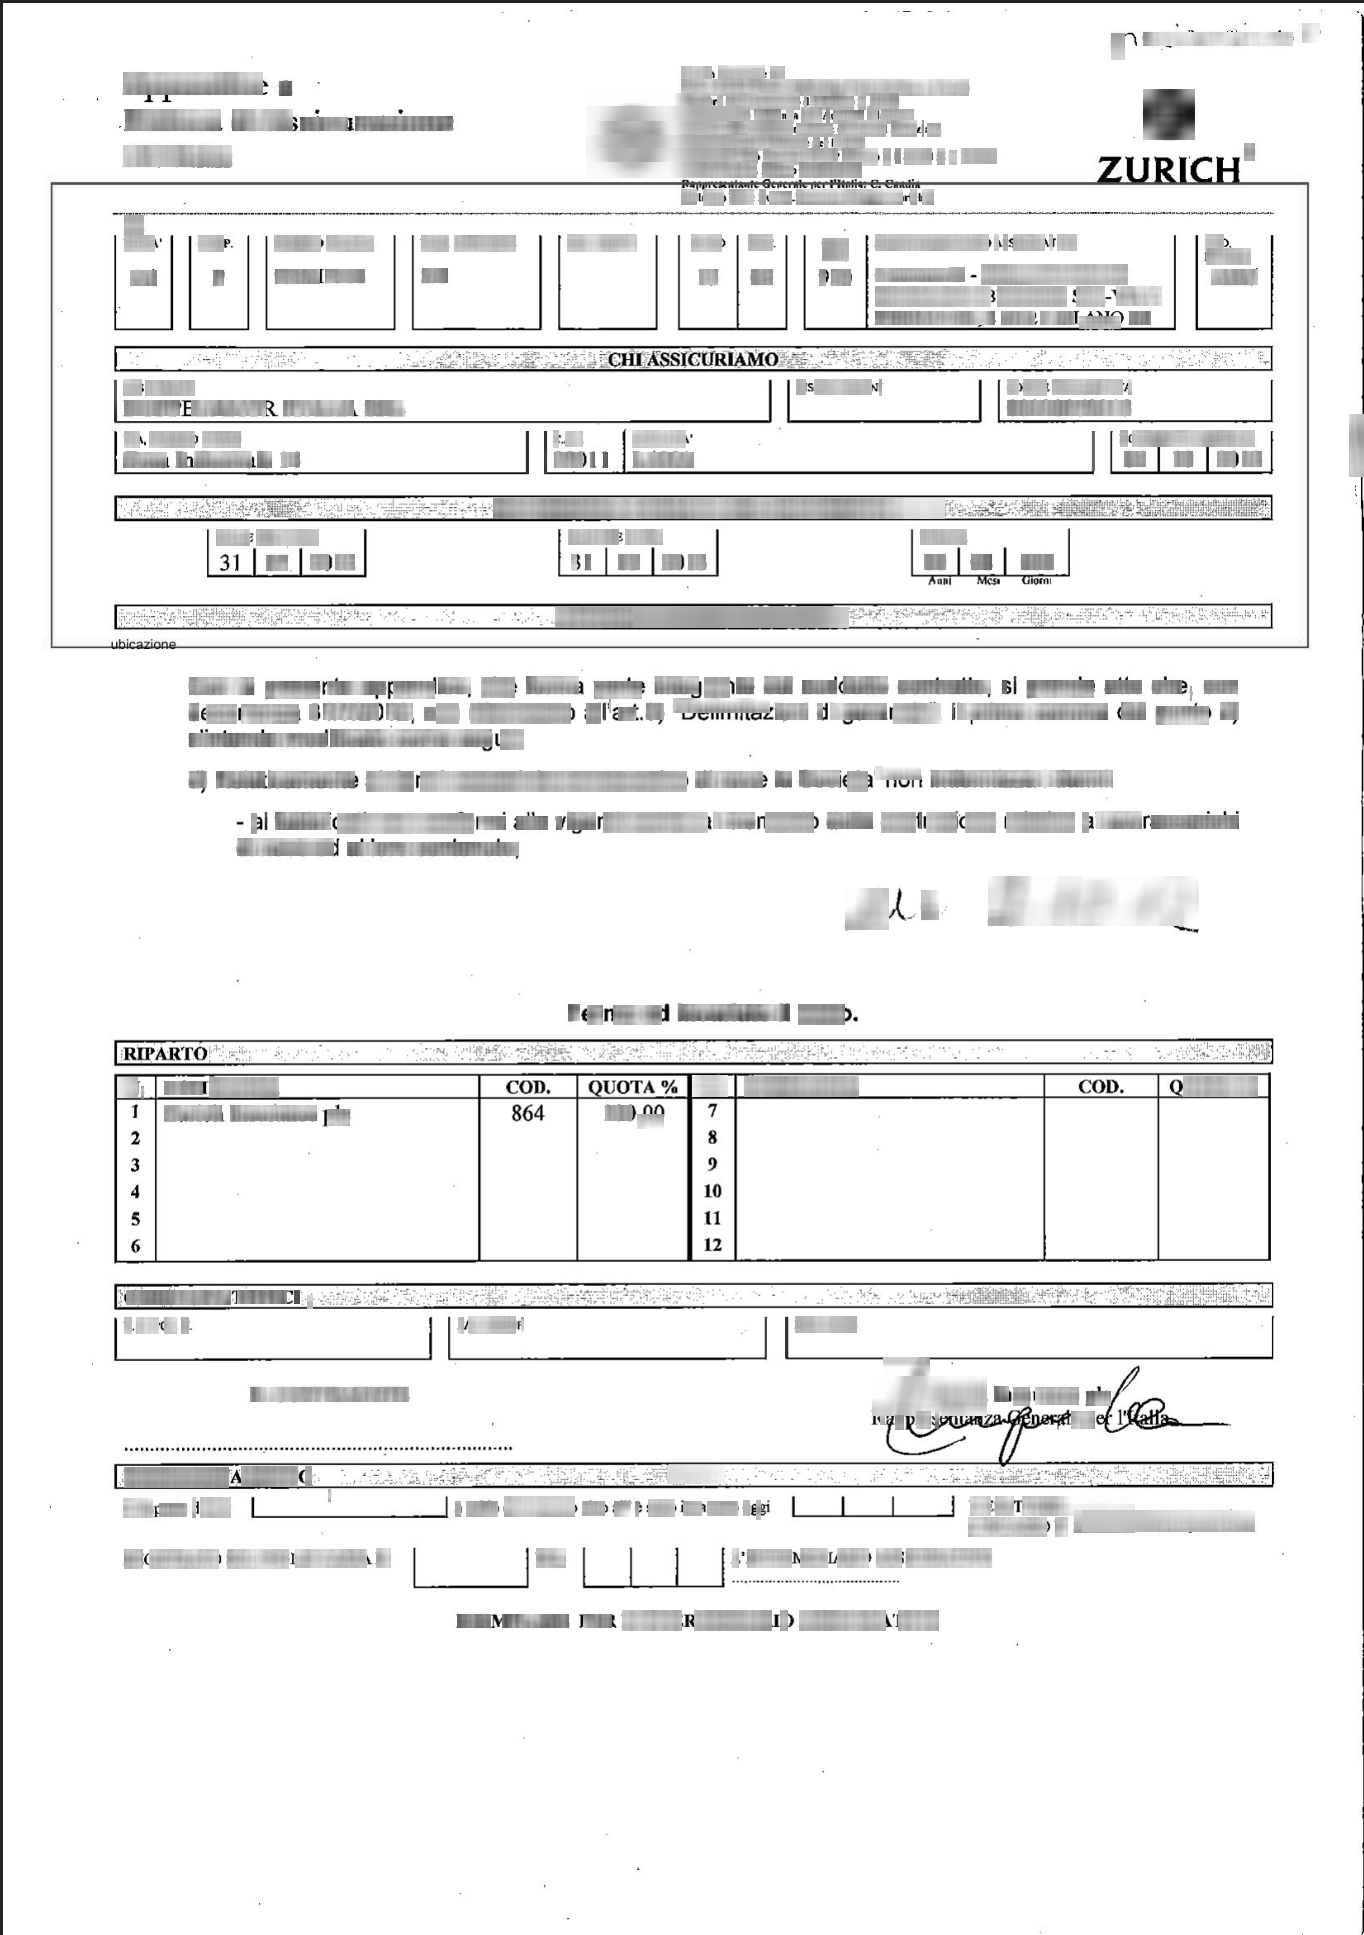
\includegraphics[width=1\columnwidth]{appendice/test3} 
    \caption{Test 3}
    \label{img:test-1}
\end{figure} 
\newpage

%============================================================================================


\begin{figure}[H]  
    \begin{minipage}{.5\columnwidth}  
        \centering  
        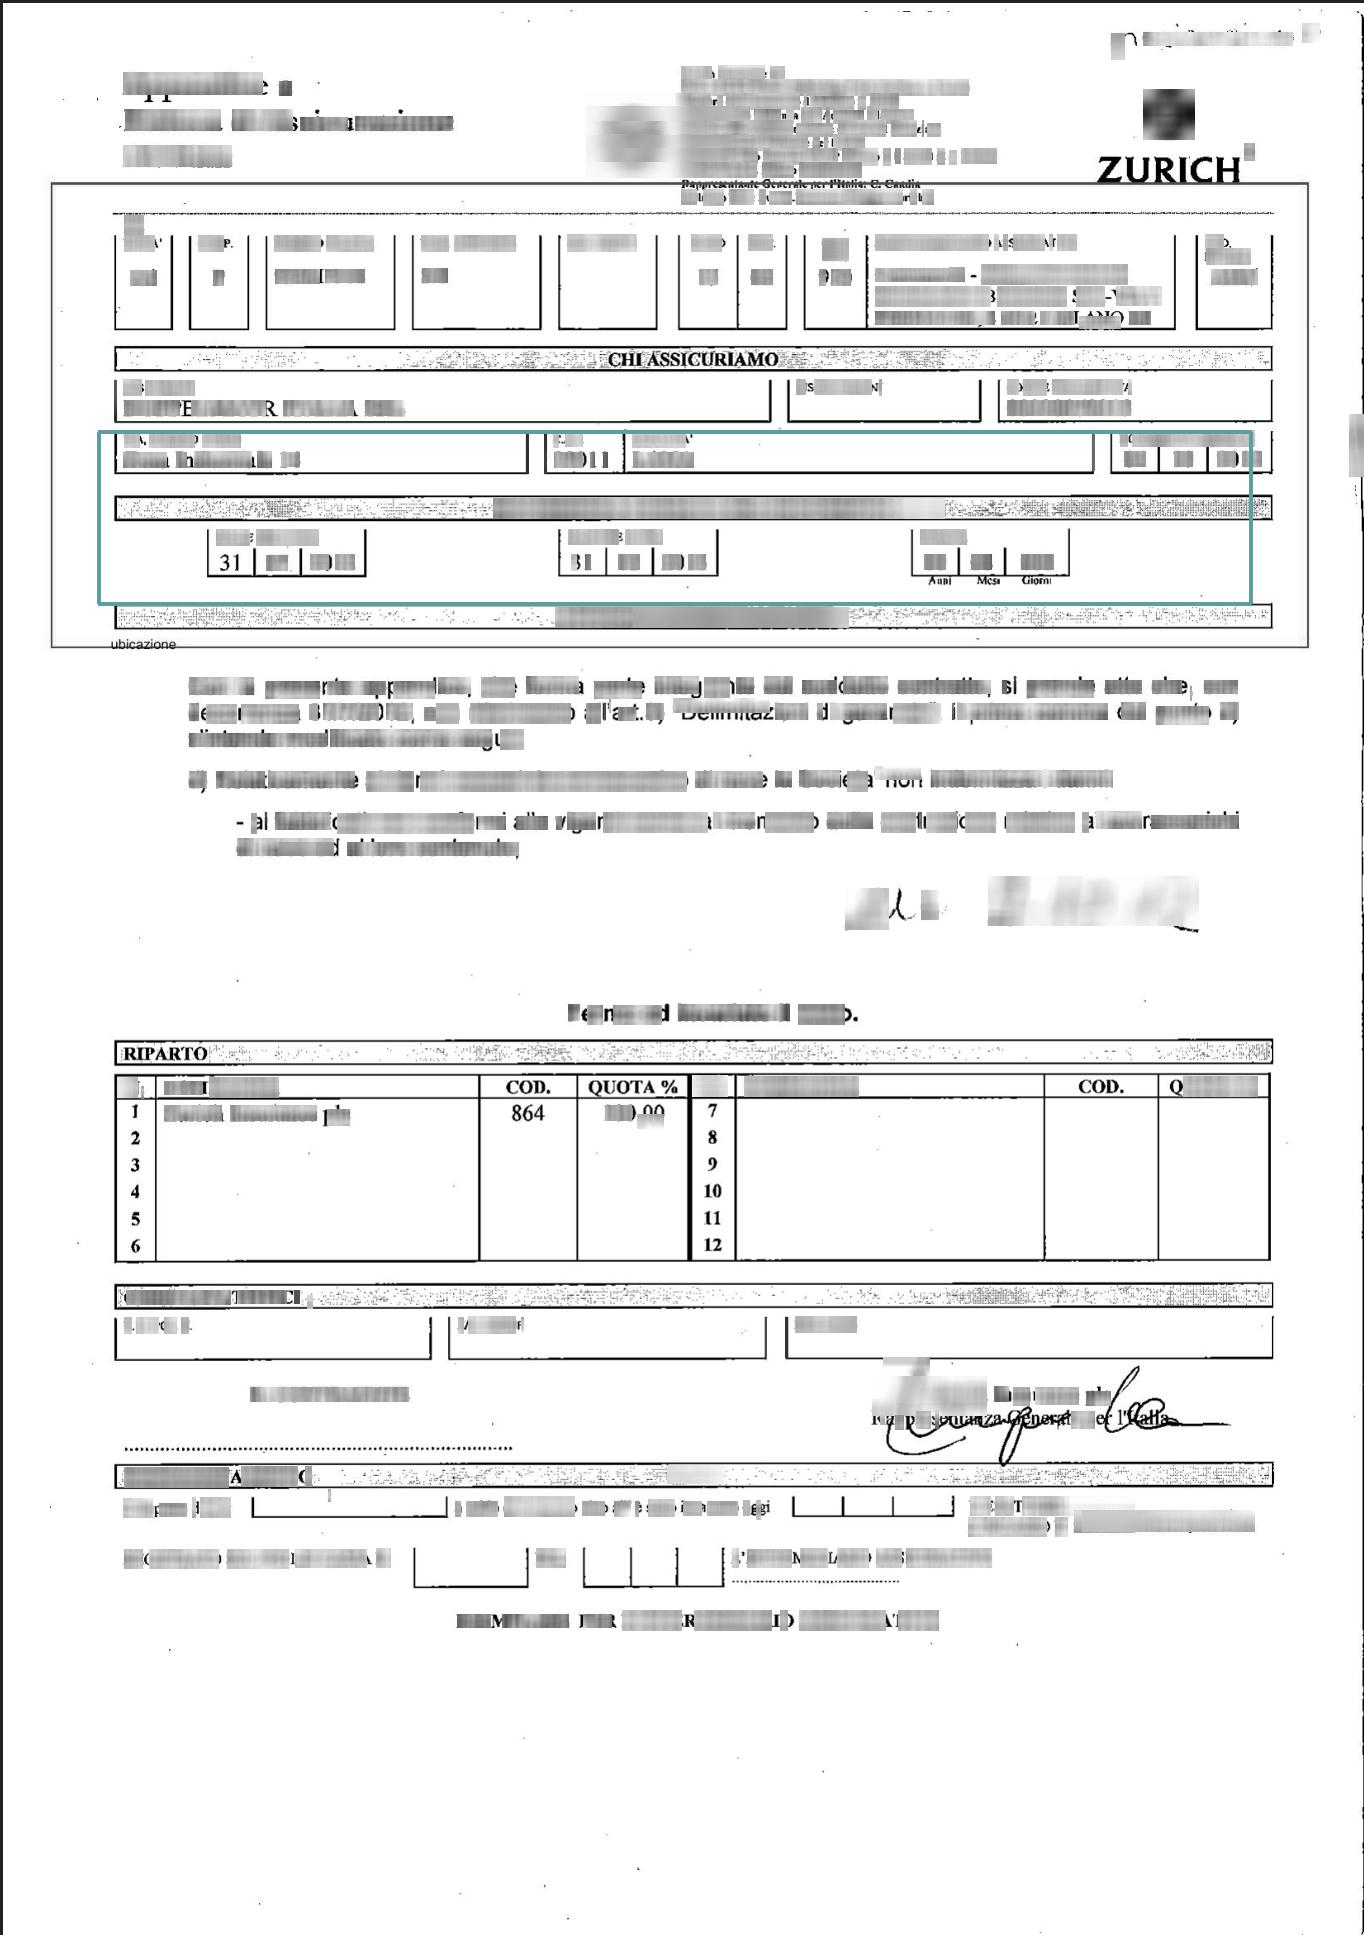
\includegraphics[width=1\columnwidth]{appendice/filtrate/test3_filtered_0_6_adam_1}  
    \end{minipage}%  
    \begin{minipage}{0.5\columnwidth}  
        \centering  
        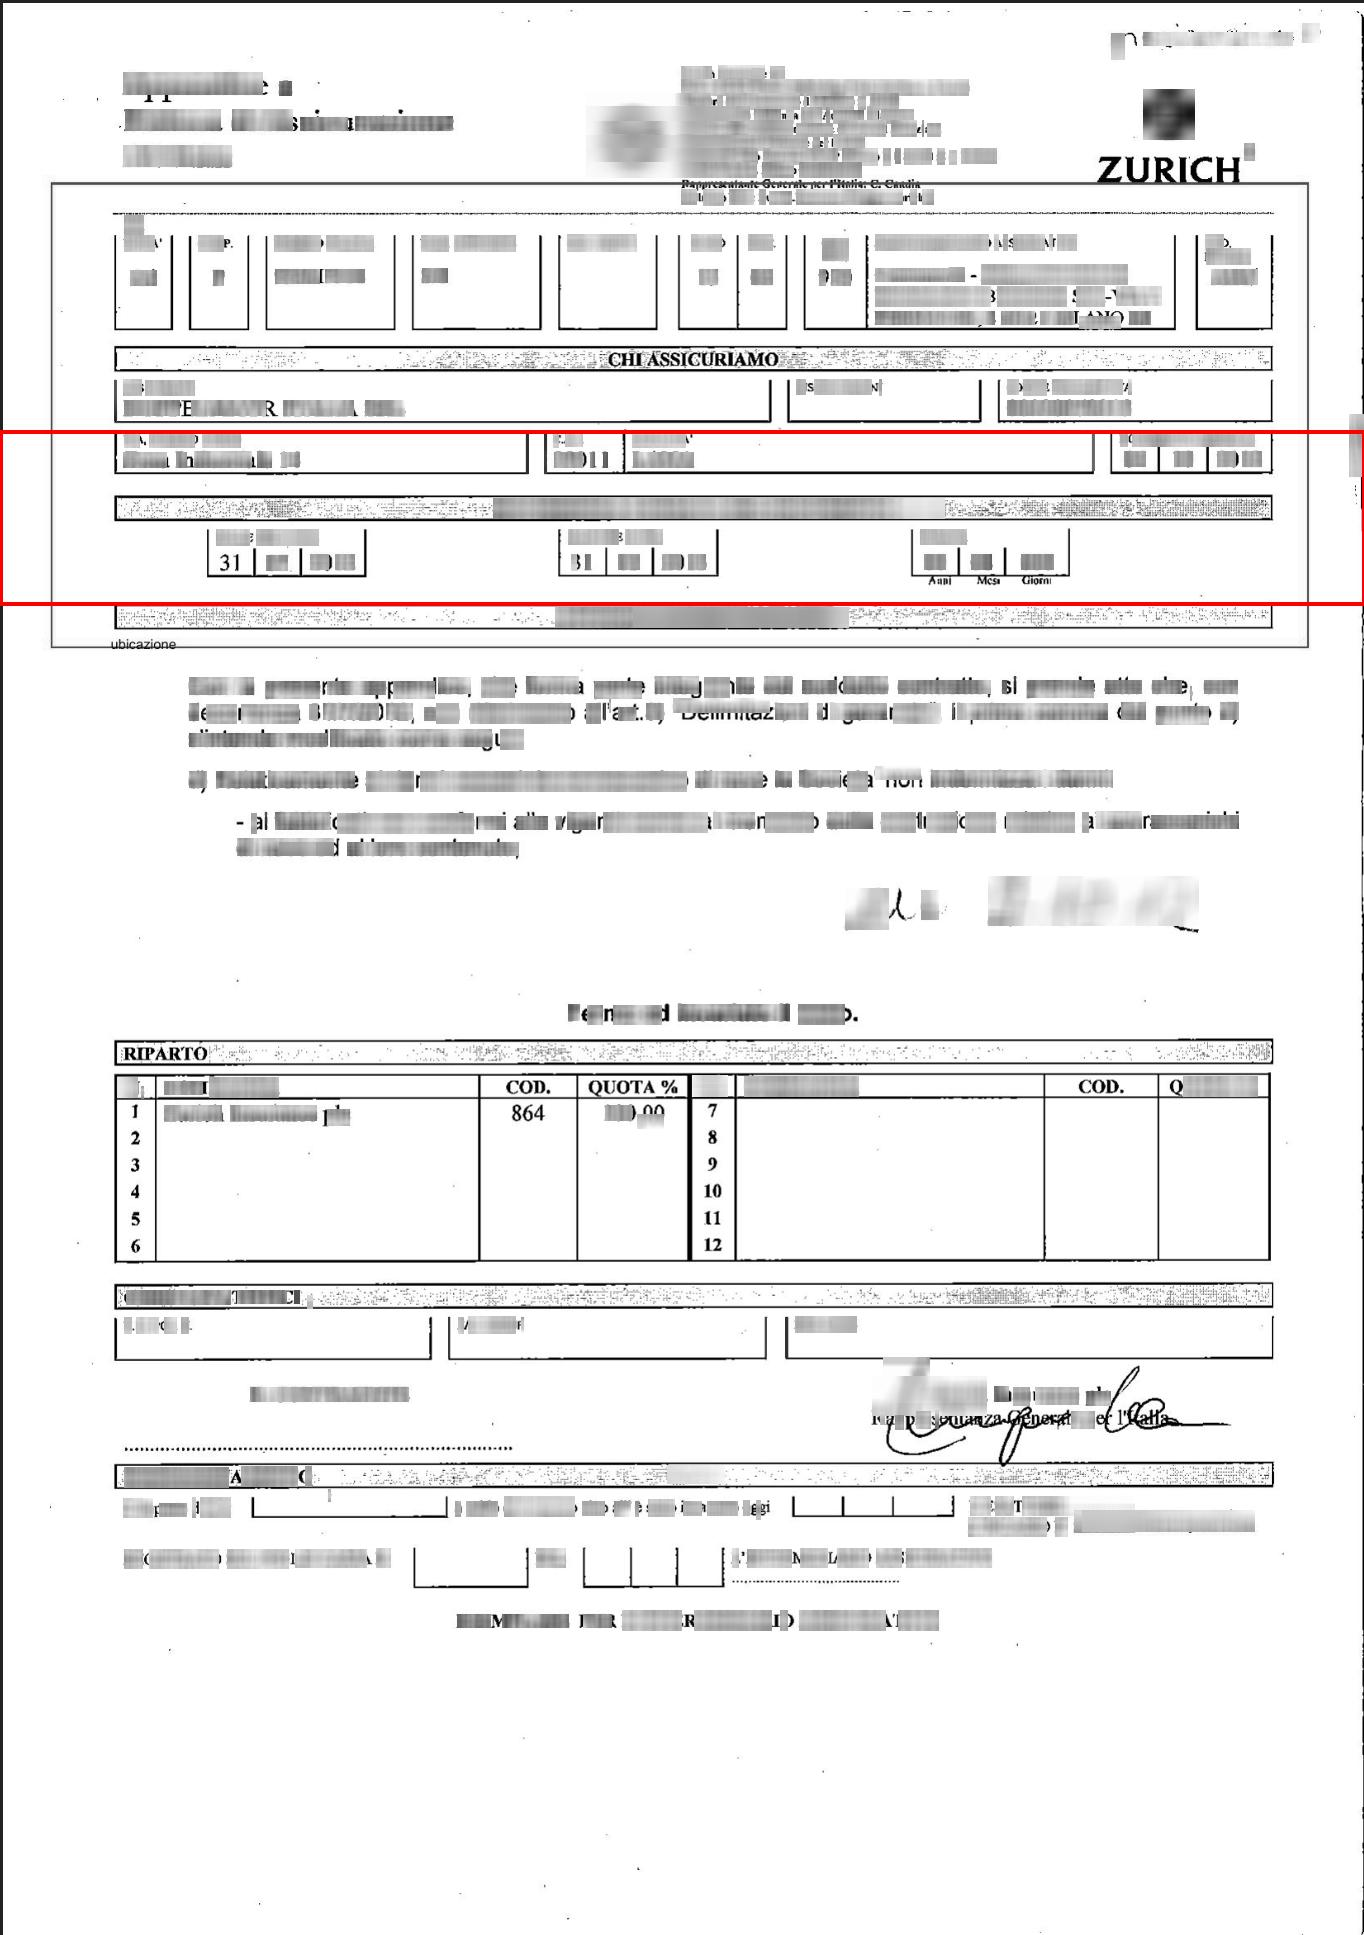
\includegraphics[width=1\columnwidth]{appendice/unite/test3_merged_0_6_adam_1}  
    \end{minipage}  
    \caption{Test 3, configurazione 1}
\end{figure}%  
Configurazione:
\begin{multicols}{2}
    \begin{lstlisting}
image_resizer {
  fixes_shape_resizer {
    width: 400
    heigth: 400
  }
}
first_stage_box_predictor {
  l2_regularizer {
    weight: 0.008
}
first_stage_nms_iou_threshold: 0.7
second_stage_box_predictor {
  l2_regularizer {
    weight: 0.004
  }
}
second_stage_post_processing {
  iou_threshold: 0.6
}
optimizer {
  adam_optimizer: {
    learning_rate: {
      manual_step_learning_rate {
        initial_learning_rate: .00008
        schedule {
          step: 4500
          learning_rate: .00004
        }
        schedule {
          step: 7000
          learning_rate: .00002
        }
        schedule {
          step: 10000
          learning_rate: .000008
        }
    ...
    }
    momentum_optimizer_value: 0.9
  }
  use_moving_average: false
}
\end{lstlisting}
\end{multicols}

%============================================================================================
\newpage
\begin{figure}[H]  
    \begin{minipage}{.5\columnwidth}  
        \centering  
        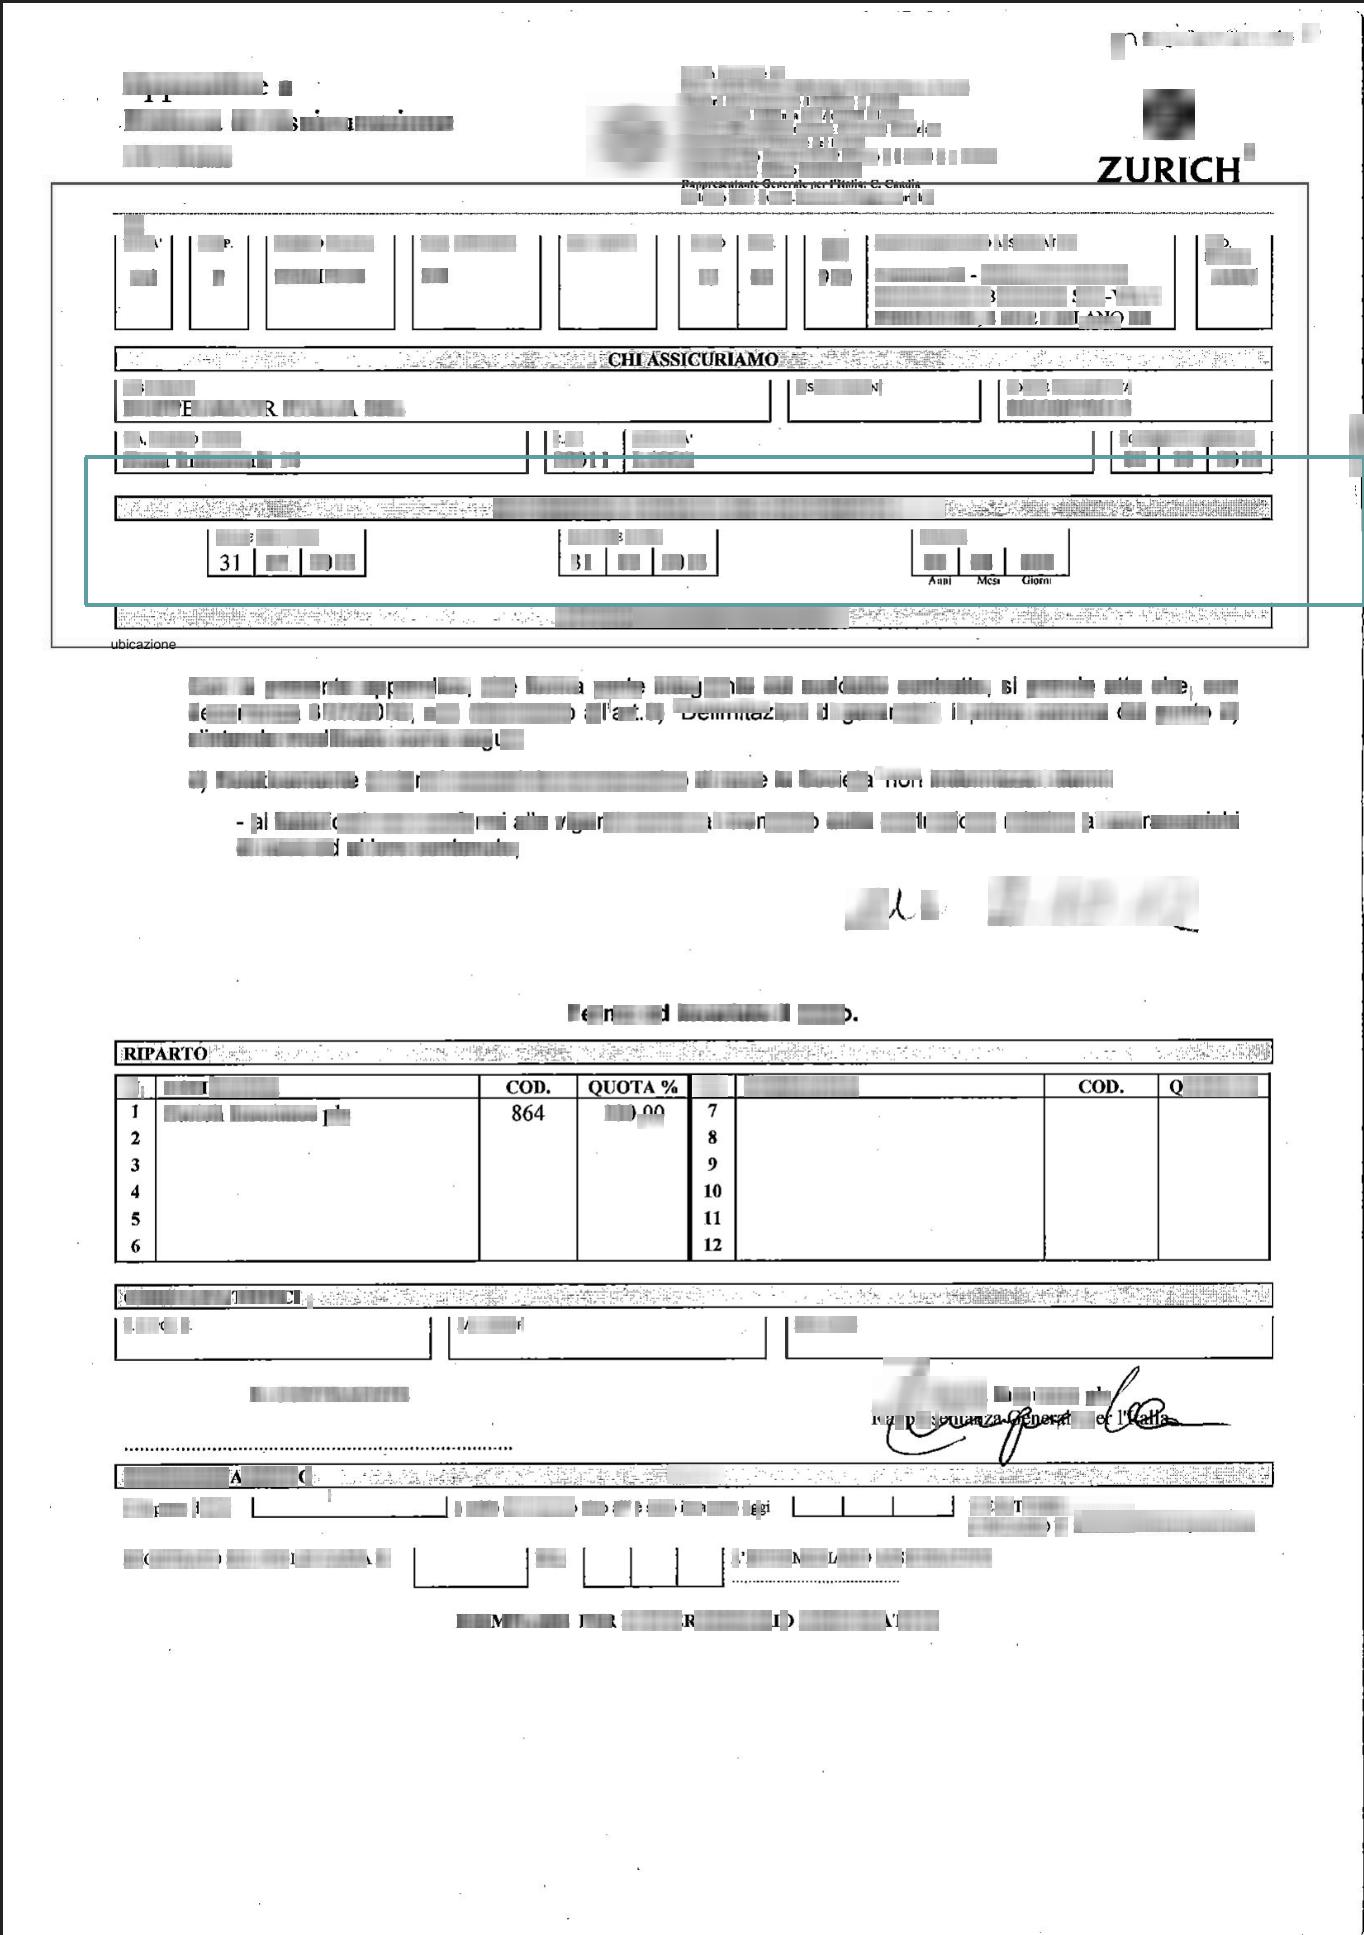
\includegraphics[width=1\columnwidth]{appendice/filtrate/test3_filtered_0_6_adam_3}  
    \end{minipage}%  
    \begin{minipage}{0.5\columnwidth}  
        \centering  
        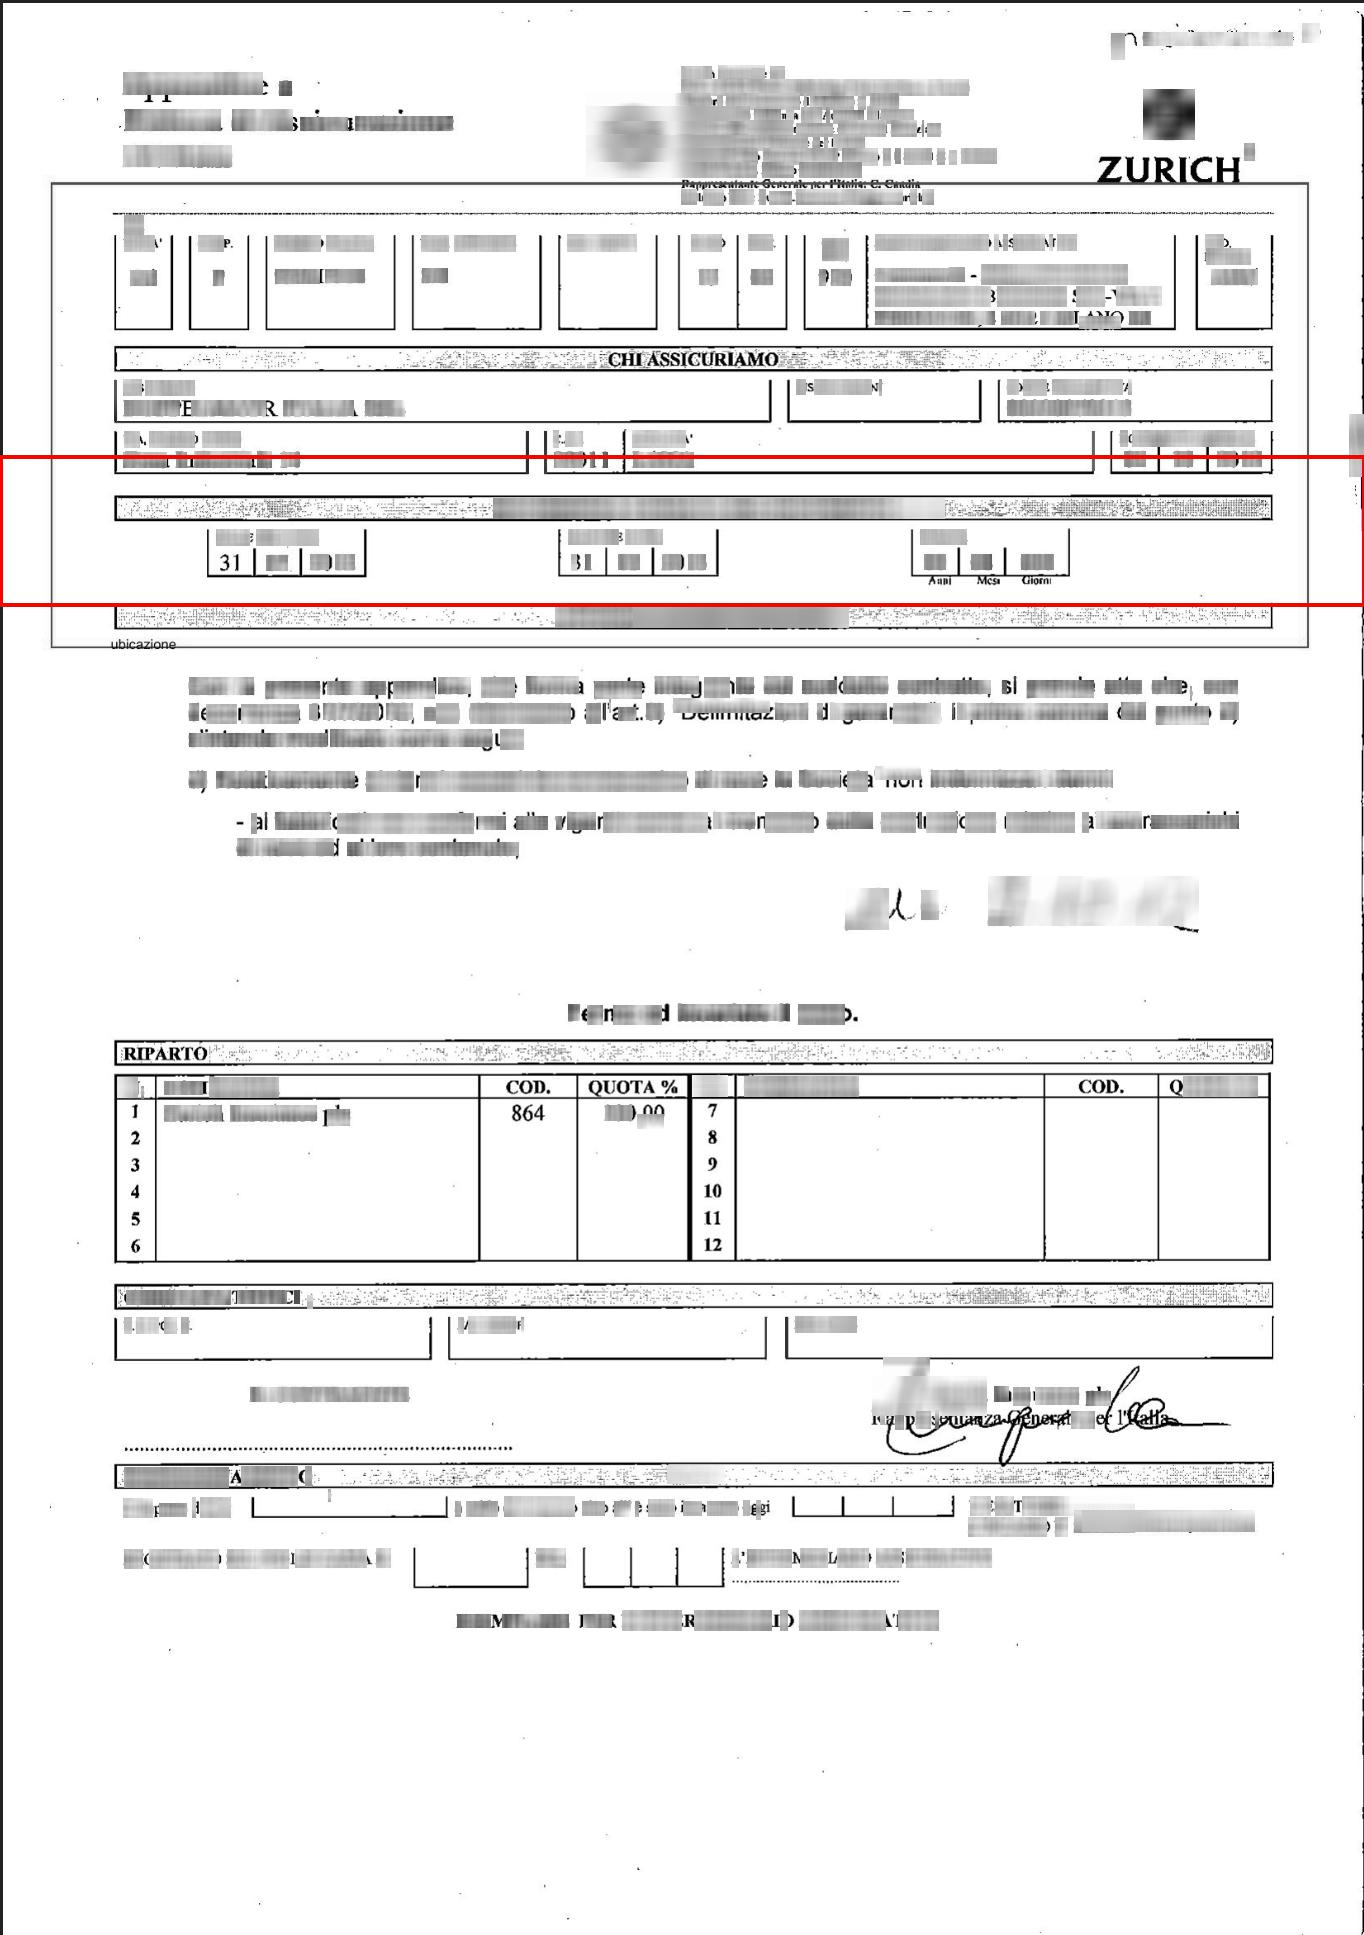
\includegraphics[width=1\columnwidth]{appendice/unite/test3_merged_0_6_adam_3}  
    \end{minipage}  
    \caption{Test 3, configurazione 2}
\end{figure}%  
Configurazione:
\begin{multicols}{2}
    \begin{lstlisting}
image_resizer {
  fixes_shape_resizer {
    width: 400
    heigth: 400
  }
}
first_stage_box_predictor {
  l2_regularizer {
    weight: 0.00001
}
first_stage_nms_iou_threshold: 0.7
second_stage_box_predictor {
  l2_regularizer {
    weight: 0.00004
  }
}
second_stage_post_processing {
  iou_threshold: 0.6
}
optimizer {
  adam_optimizer: {
    learning_rate: {
      exponential_decay_learning_rate {
        initial_learning_rate: 0.0001
          decay_steps: 600
          decay_factor: 0.95
        }
      }
    ...
  use_moving_average: false
}
    \end{lstlisting}
\end{multicols}

%============================================================================================
\newpage
\begin{figure}[H]  
    \begin{minipage}{.5\columnwidth}  
        \centering  
        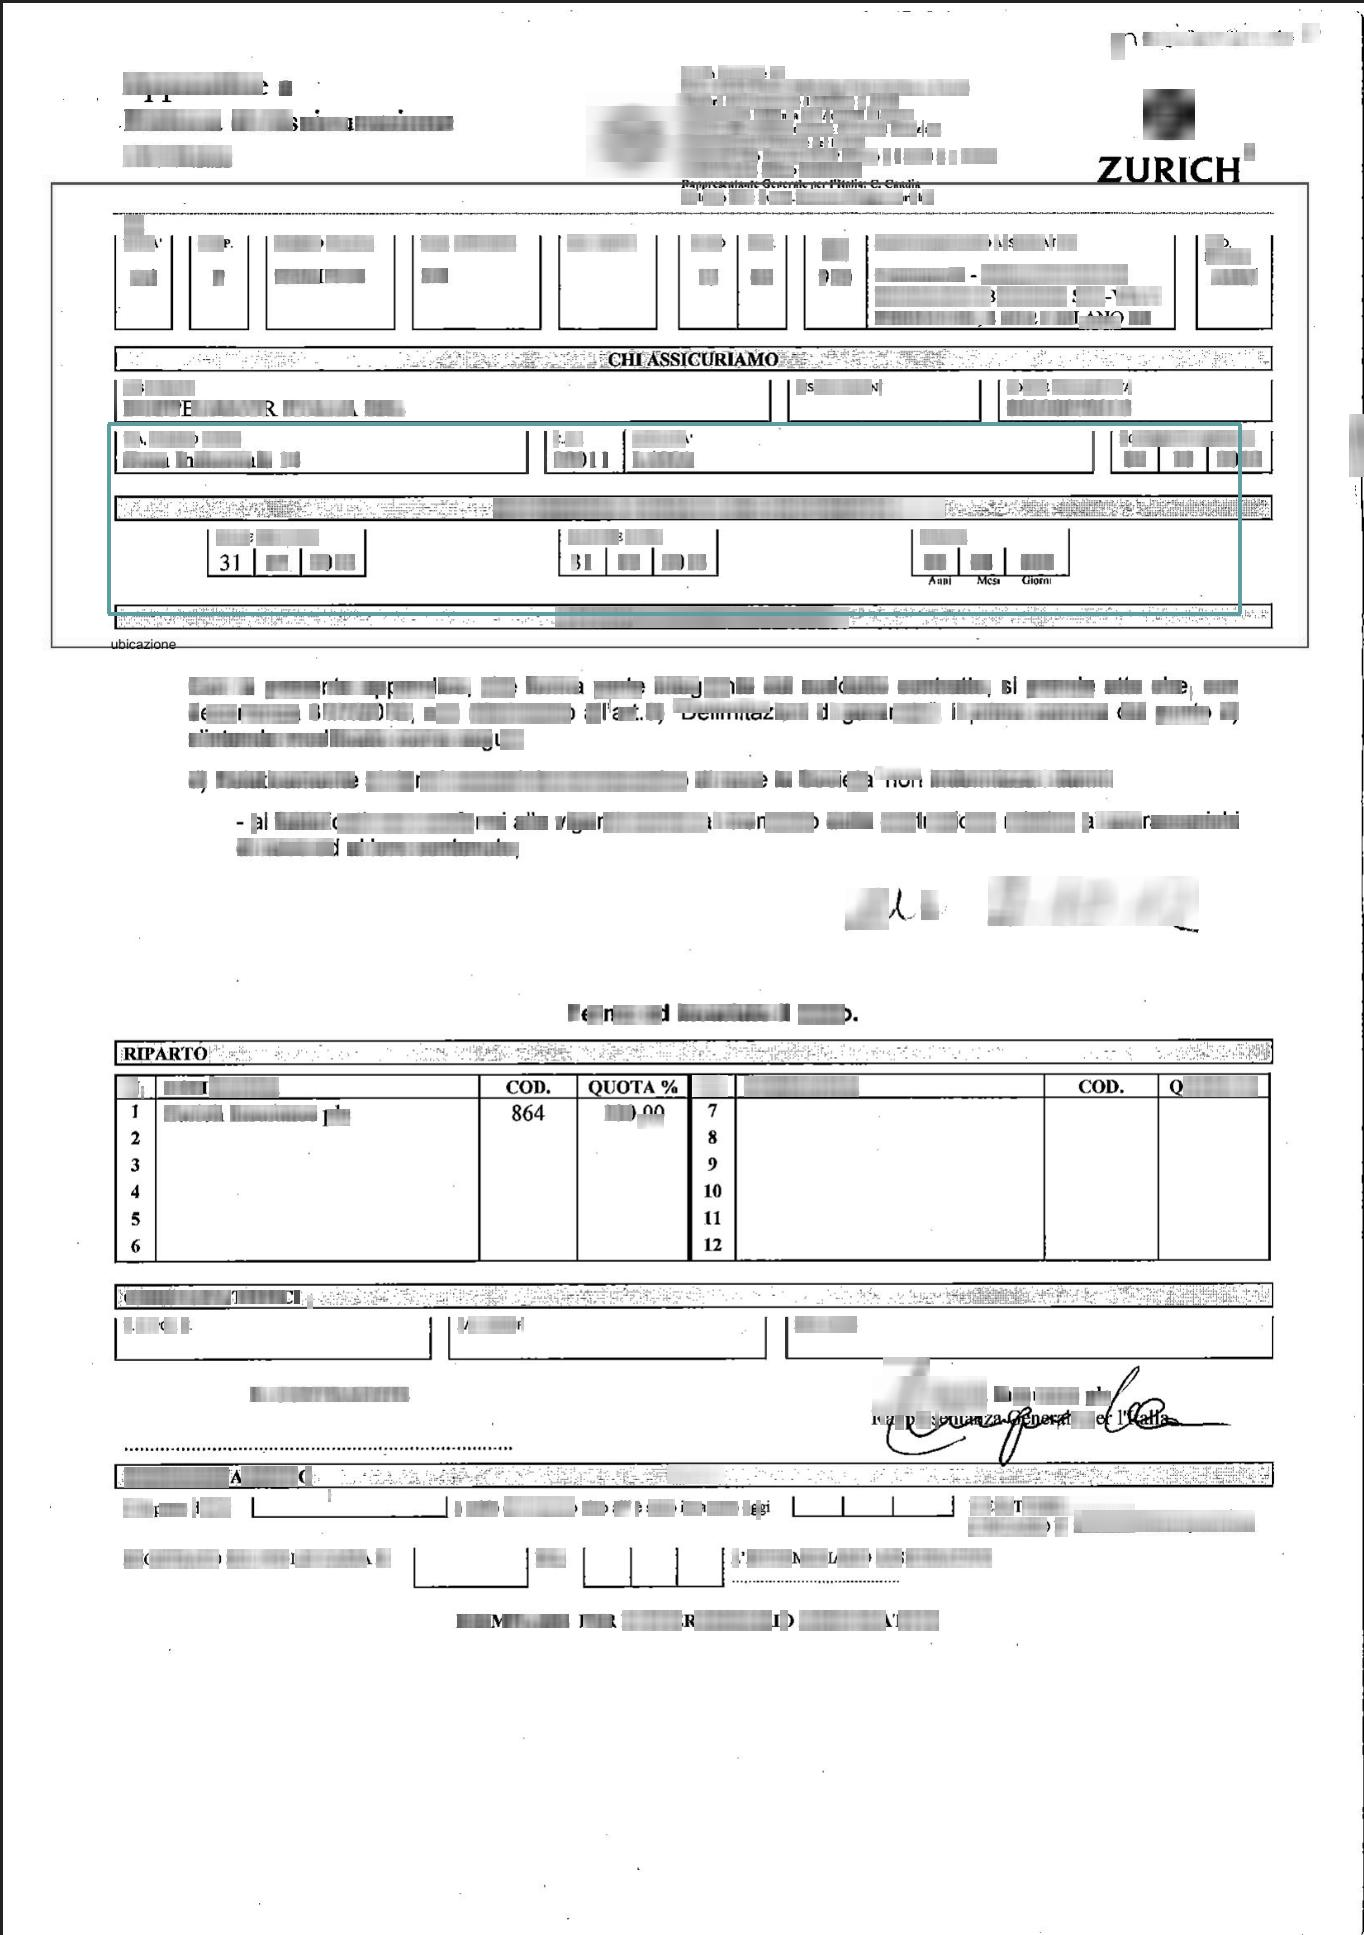
\includegraphics[width=1\columnwidth]{appendice/filtrate/test3_filtered_0_6_adam_4}  
    \end{minipage}%  
    \begin{minipage}{0.5\columnwidth}  
        \centering  
        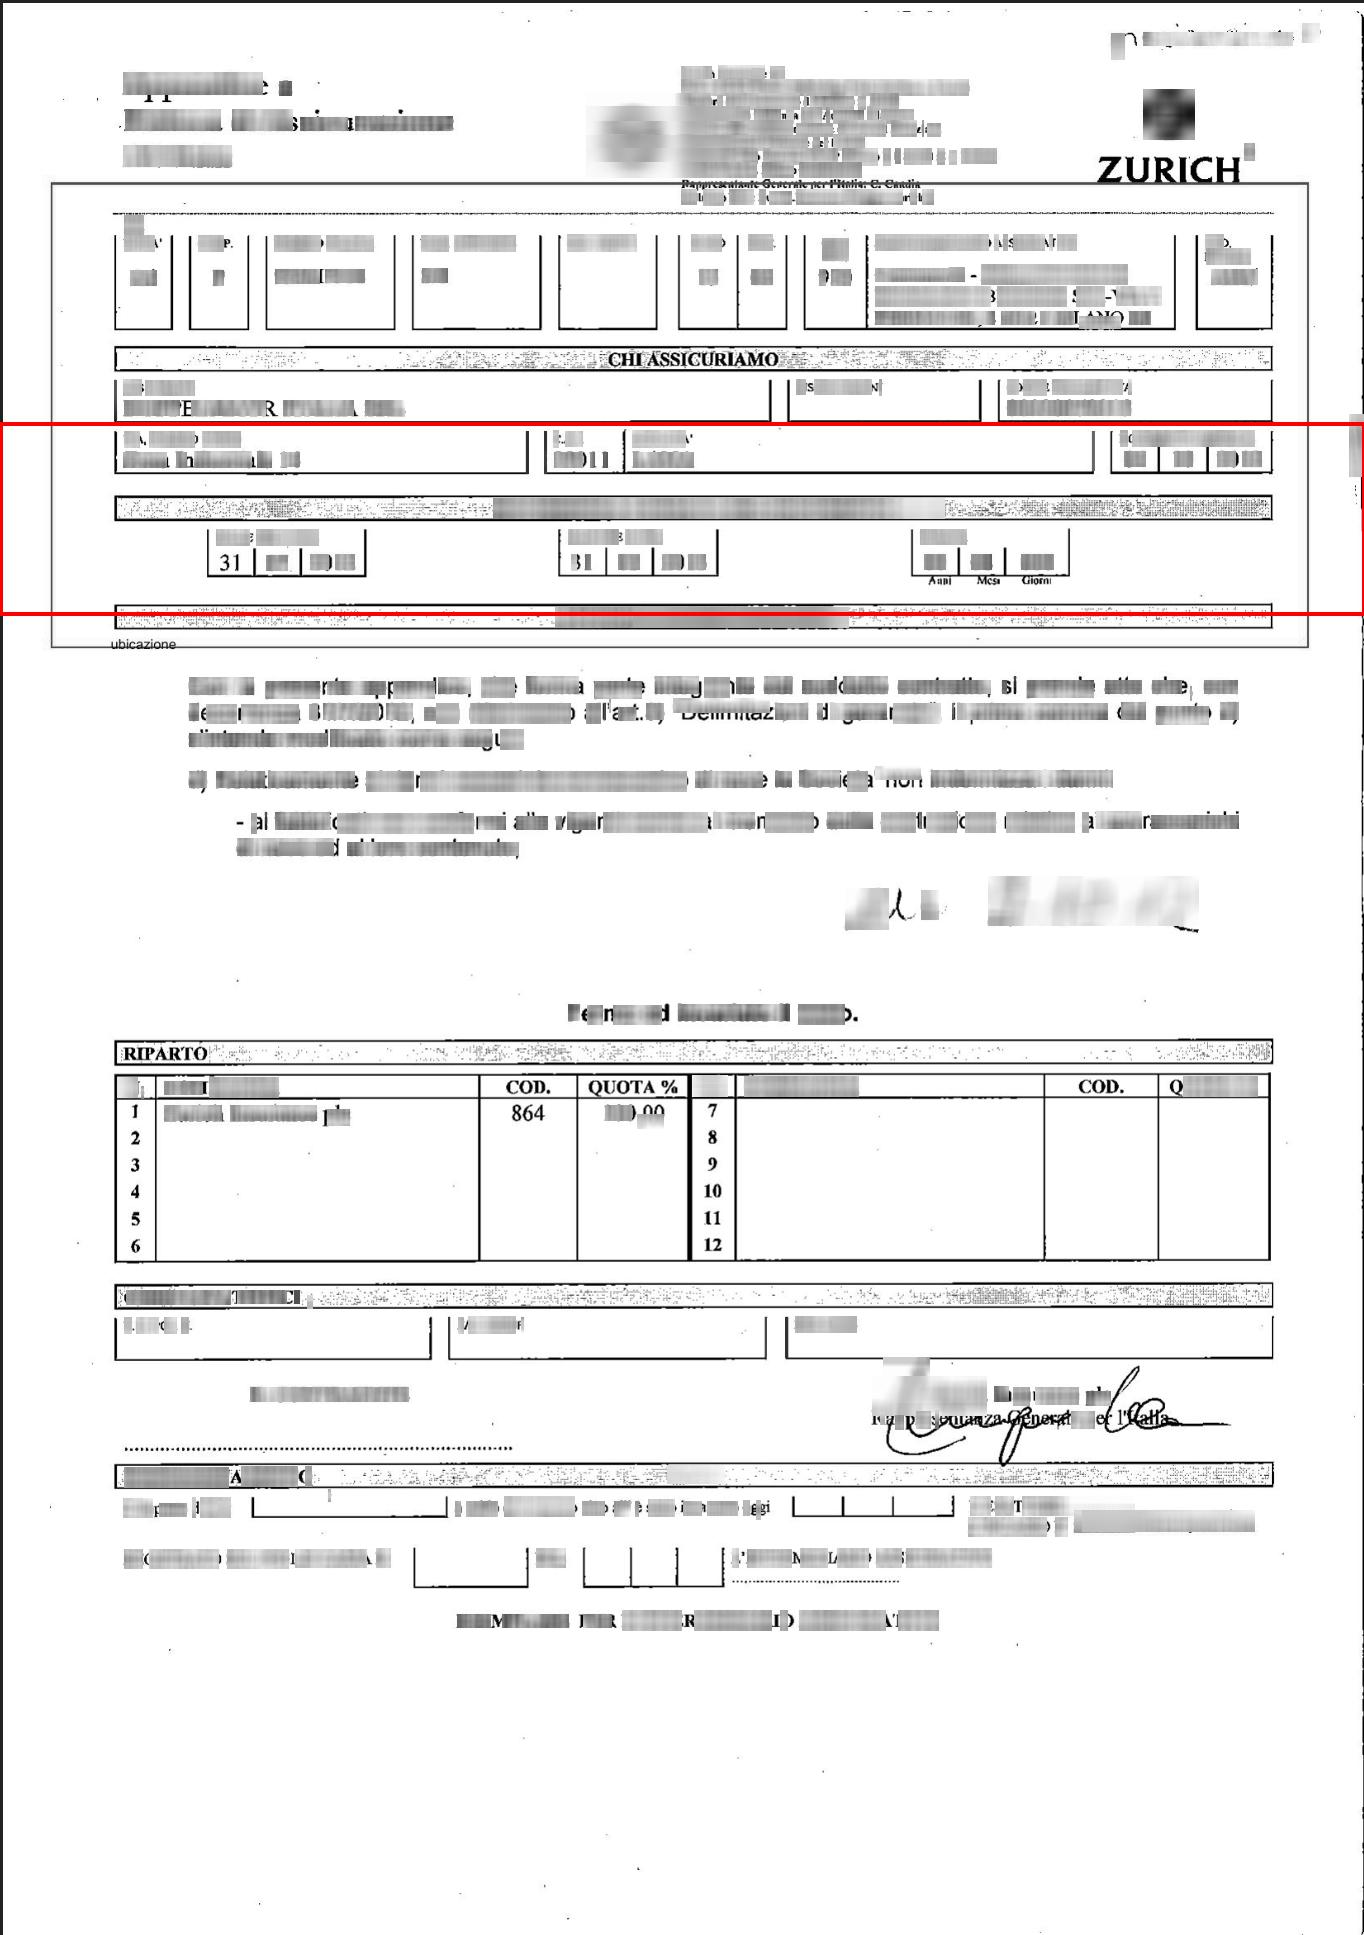
\includegraphics[width=1\columnwidth]{appendice/unite/test3_merged_0_6_adam_4}  
    \end{minipage}  
    \caption{Test 3, configurazione 3}
\end{figure}%  
Configurazione:
\begin{multicols}{2}
    \begin{lstlisting}
image_resizer {
  fixes_shape_resizer {
    width: 400
    heigth: 400
  }
}
first_stage_box_predictor {
  l2_regularizer {
    weight: 0.04
}
first_stage_nms_iou_threshold: 0.7
second_stage_box_predictor {
  l2_regularizer {
    weight: 0.004
  }
}
second_stage_post_processing {
  iou_threshold: 0.6
}
optimizer {
  adam_optimizer: {
    learning_rate: {
      exponential_decay_learning_rate {
        initial_learning_rate: 0.0001
          decay_steps: 450
          decay_factor: 0.9
        }
      }
    ...
  use_moving_average: false
}
    \end{lstlisting}
\end{multicols}

%============================================================================================
\newpage
\begin{figure}[H]  
    \begin{minipage}{.5\columnwidth}  
        \centering  
        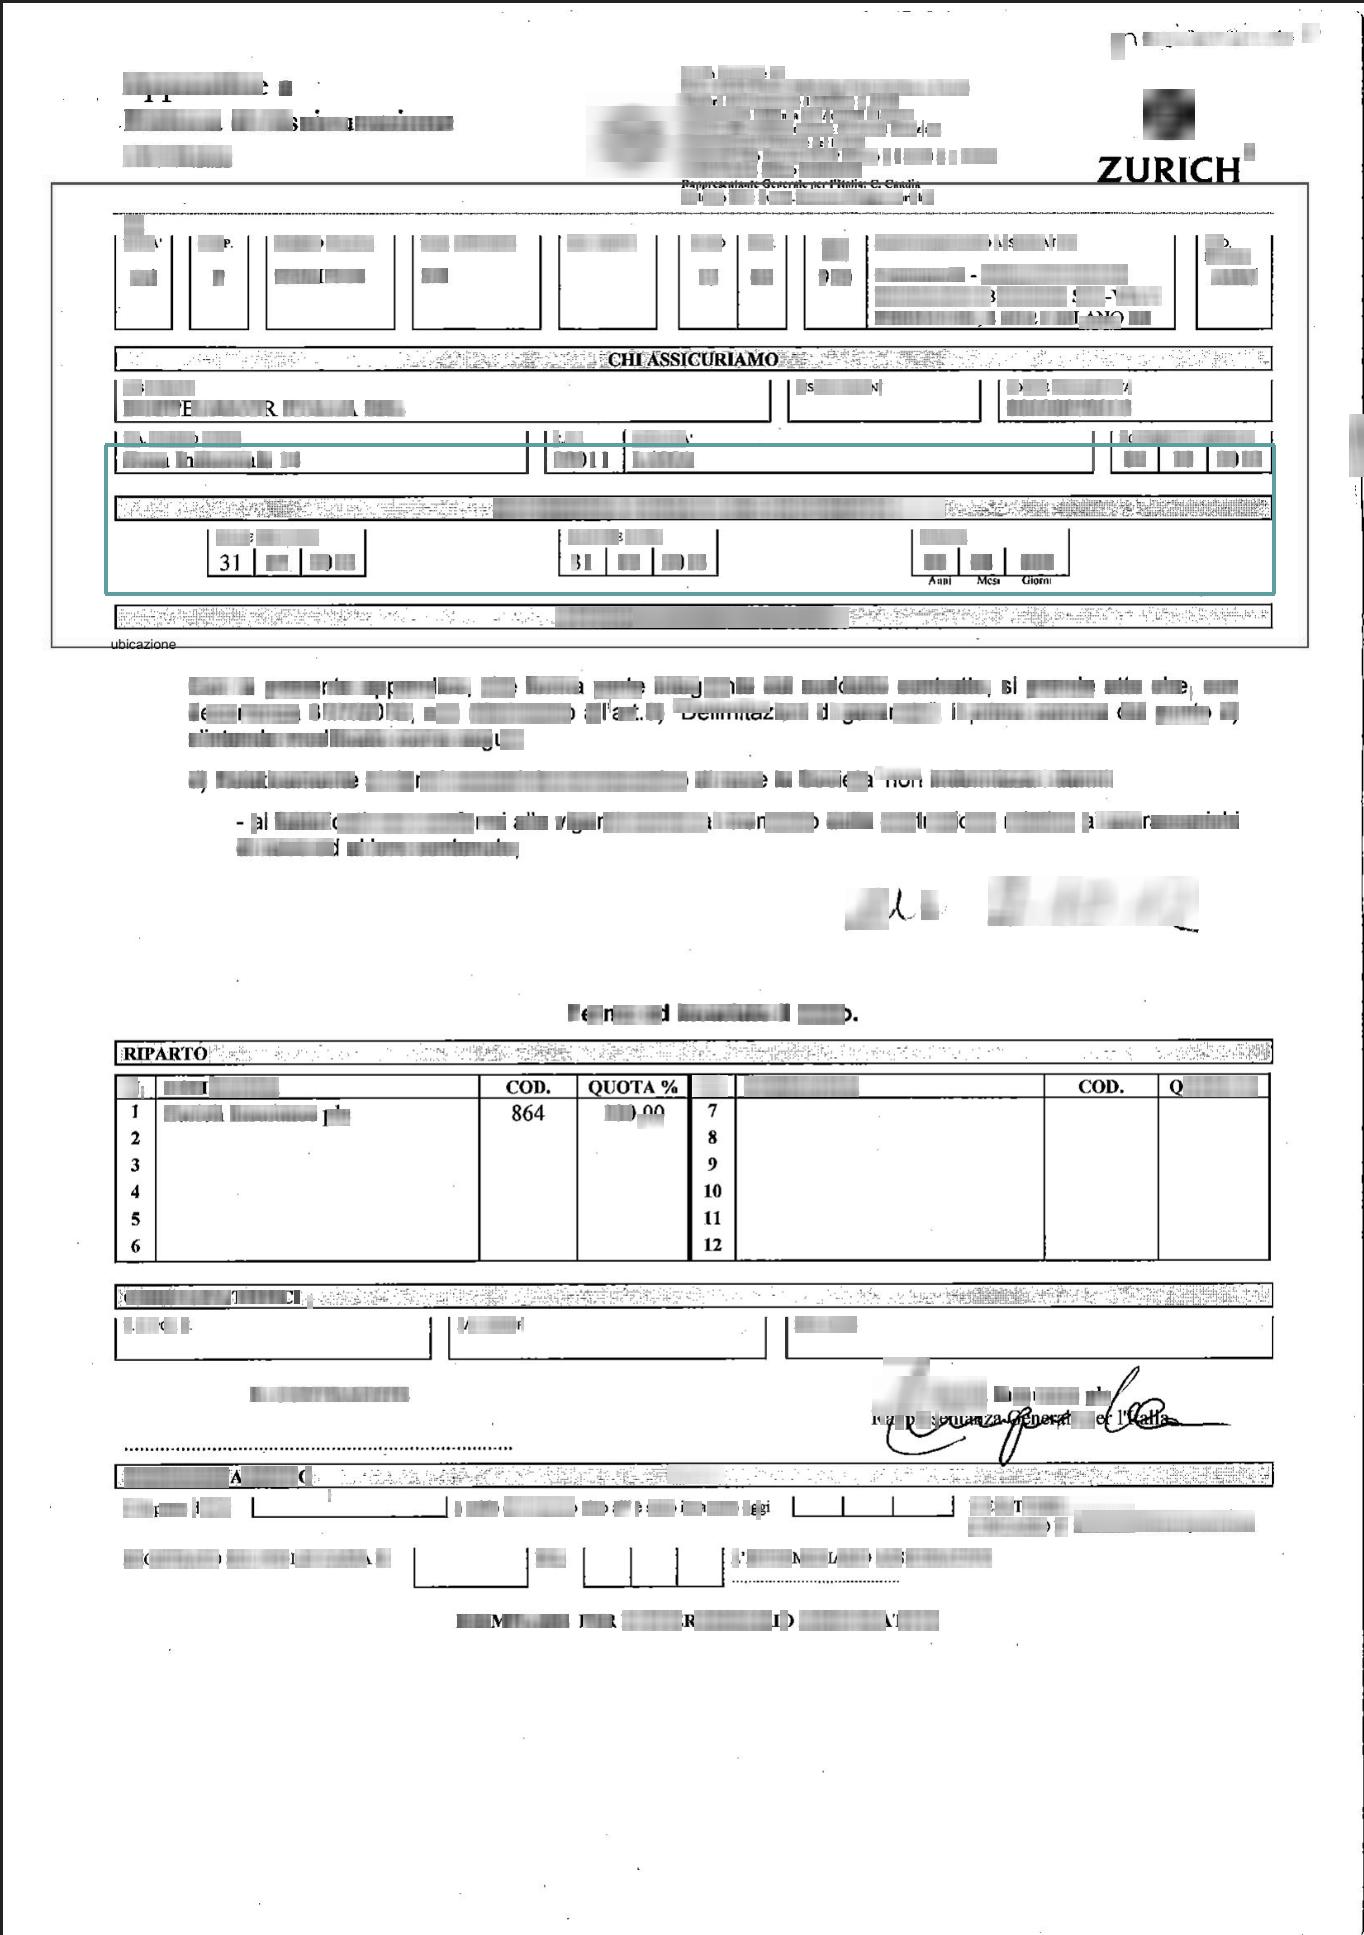
\includegraphics[width=1\columnwidth]{appendice/filtrate/test3_filtered_0_6_momentum_1}  
    \end{minipage}%  
    \begin{minipage}{0.5\columnwidth}  
        \centering  
        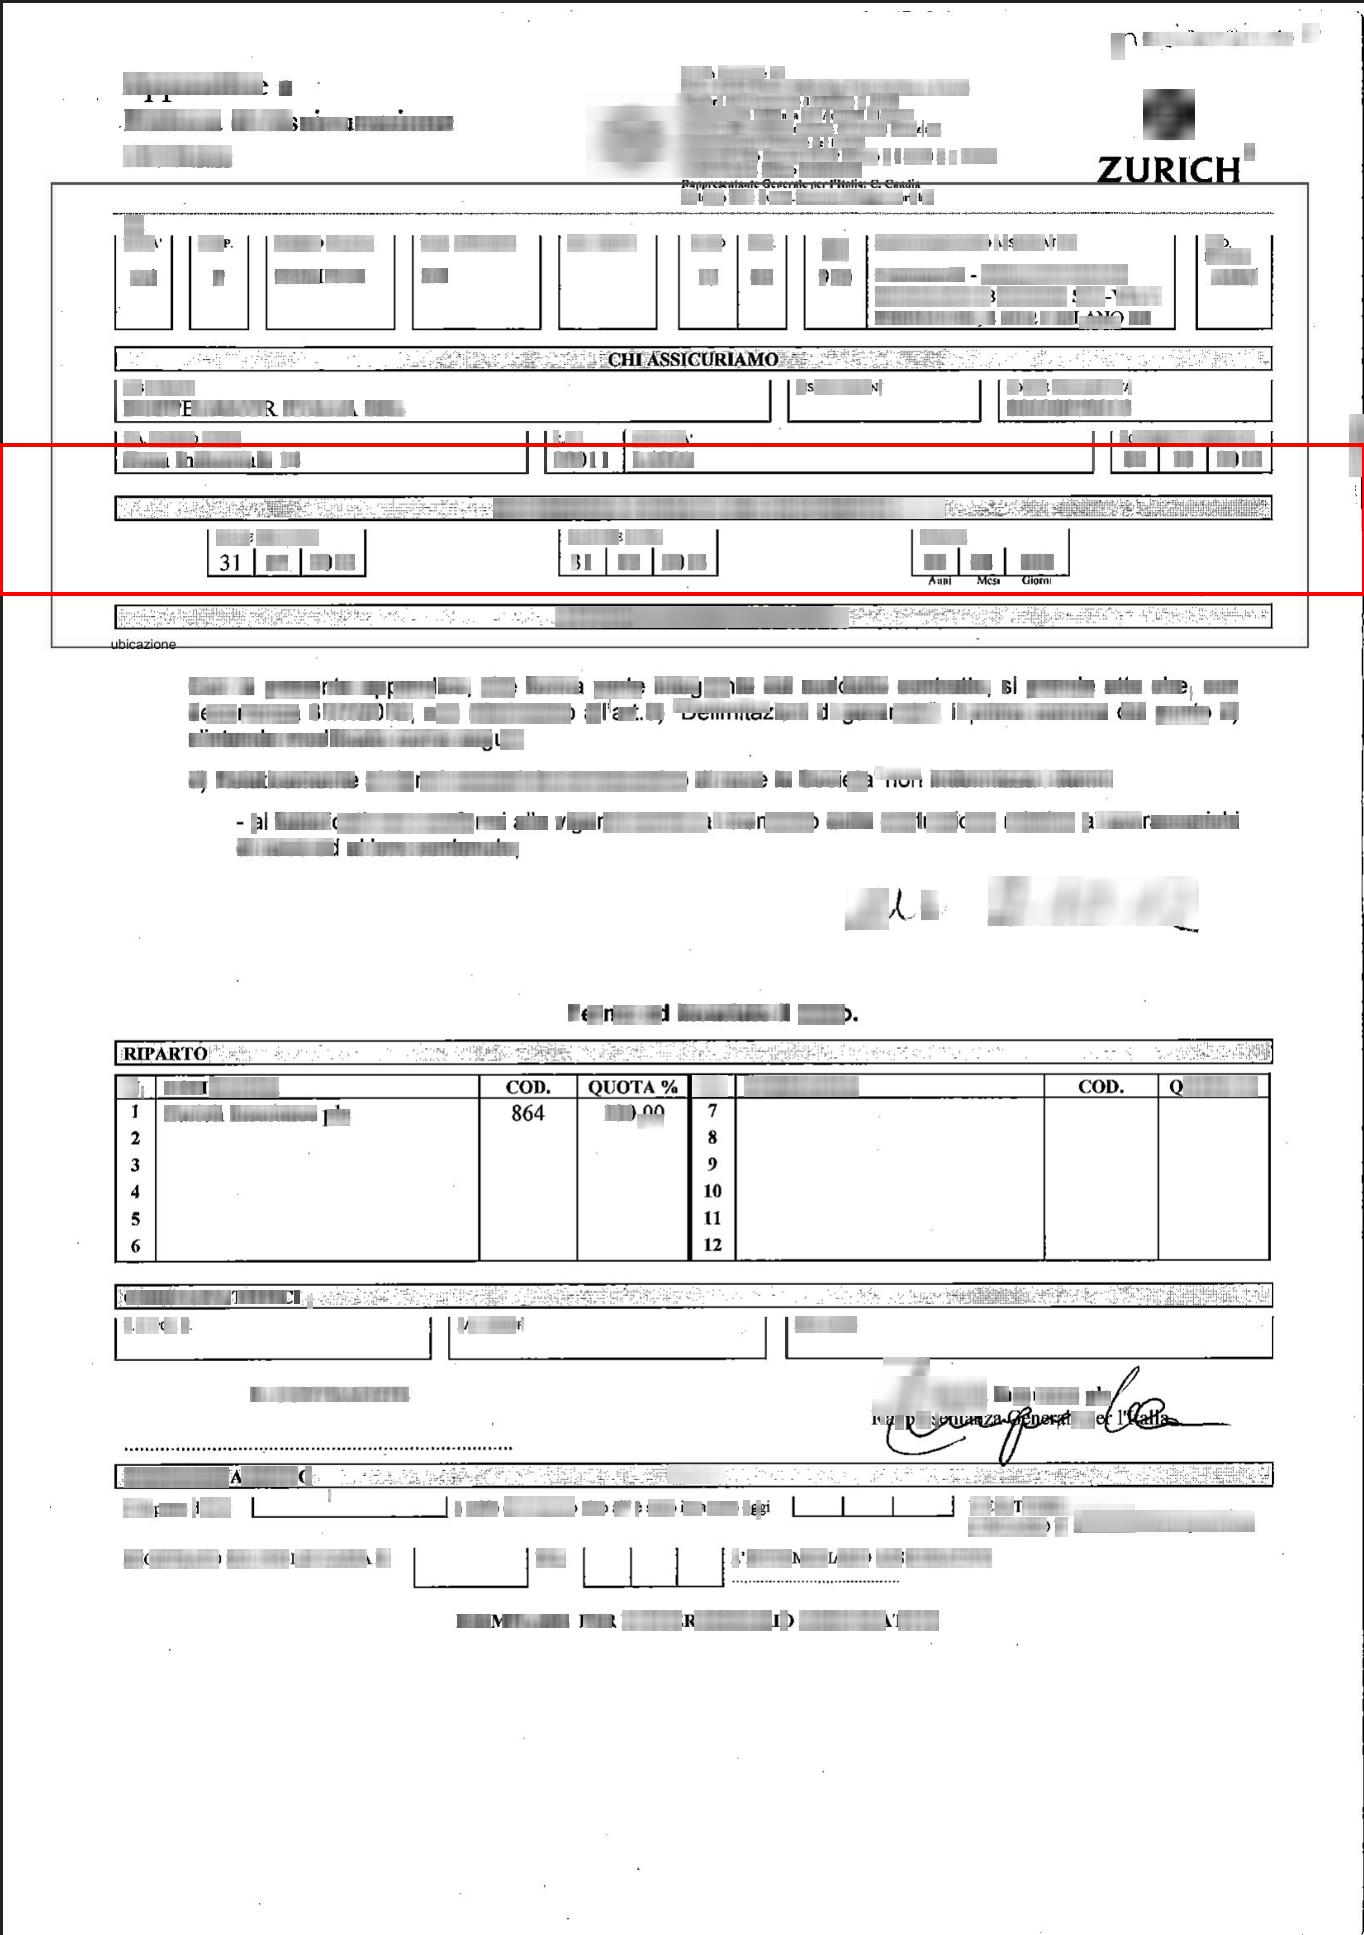
\includegraphics[width=1\columnwidth]{appendice/unite/test3_merged_0_6_momentum_1}  
    \end{minipage}  
    \caption{Test 3, configurazione 4}
\end{figure}%  
Configurazione:
\begin{multicols}{2}
    \begin{lstlisting}
image_resizer {
  fixes_shape_resizer {
    width: 400
    heigth: 400
  }
}
first_stage_box_predictor {
  l2_regularizer {
    weight: 0.00001
}
first_stage_nms_iou_threshold: 0.7
second_stage_box_predictor {
  l2_regularizer {
    weight: 0.00004
  }
}
second_stage_post_processing {
  iou_threshold: 0.6
}
optimizer {
  adam_optimizer: {
    learning_rate: {
      manual_step_learning_rate {
        initial_learning_rate: 0.0008
        schedule {
          step: 4500
          learning_rate: .0008
        }
        schedule {
          step: 7000
          learning_rate: .0004
        }
        schedule {
          step: 10000
          learning_rate: .00008
        }
    ...
    }
    momentum_optimizer_value: 0.9
  }
  use_moving_average: false
}
    \end{lstlisting}
\end{multicols}
%============================================================================================

\newpage
\begin{figure}[H]  
    \begin{minipage}{.5\columnwidth}  
        \centering  
        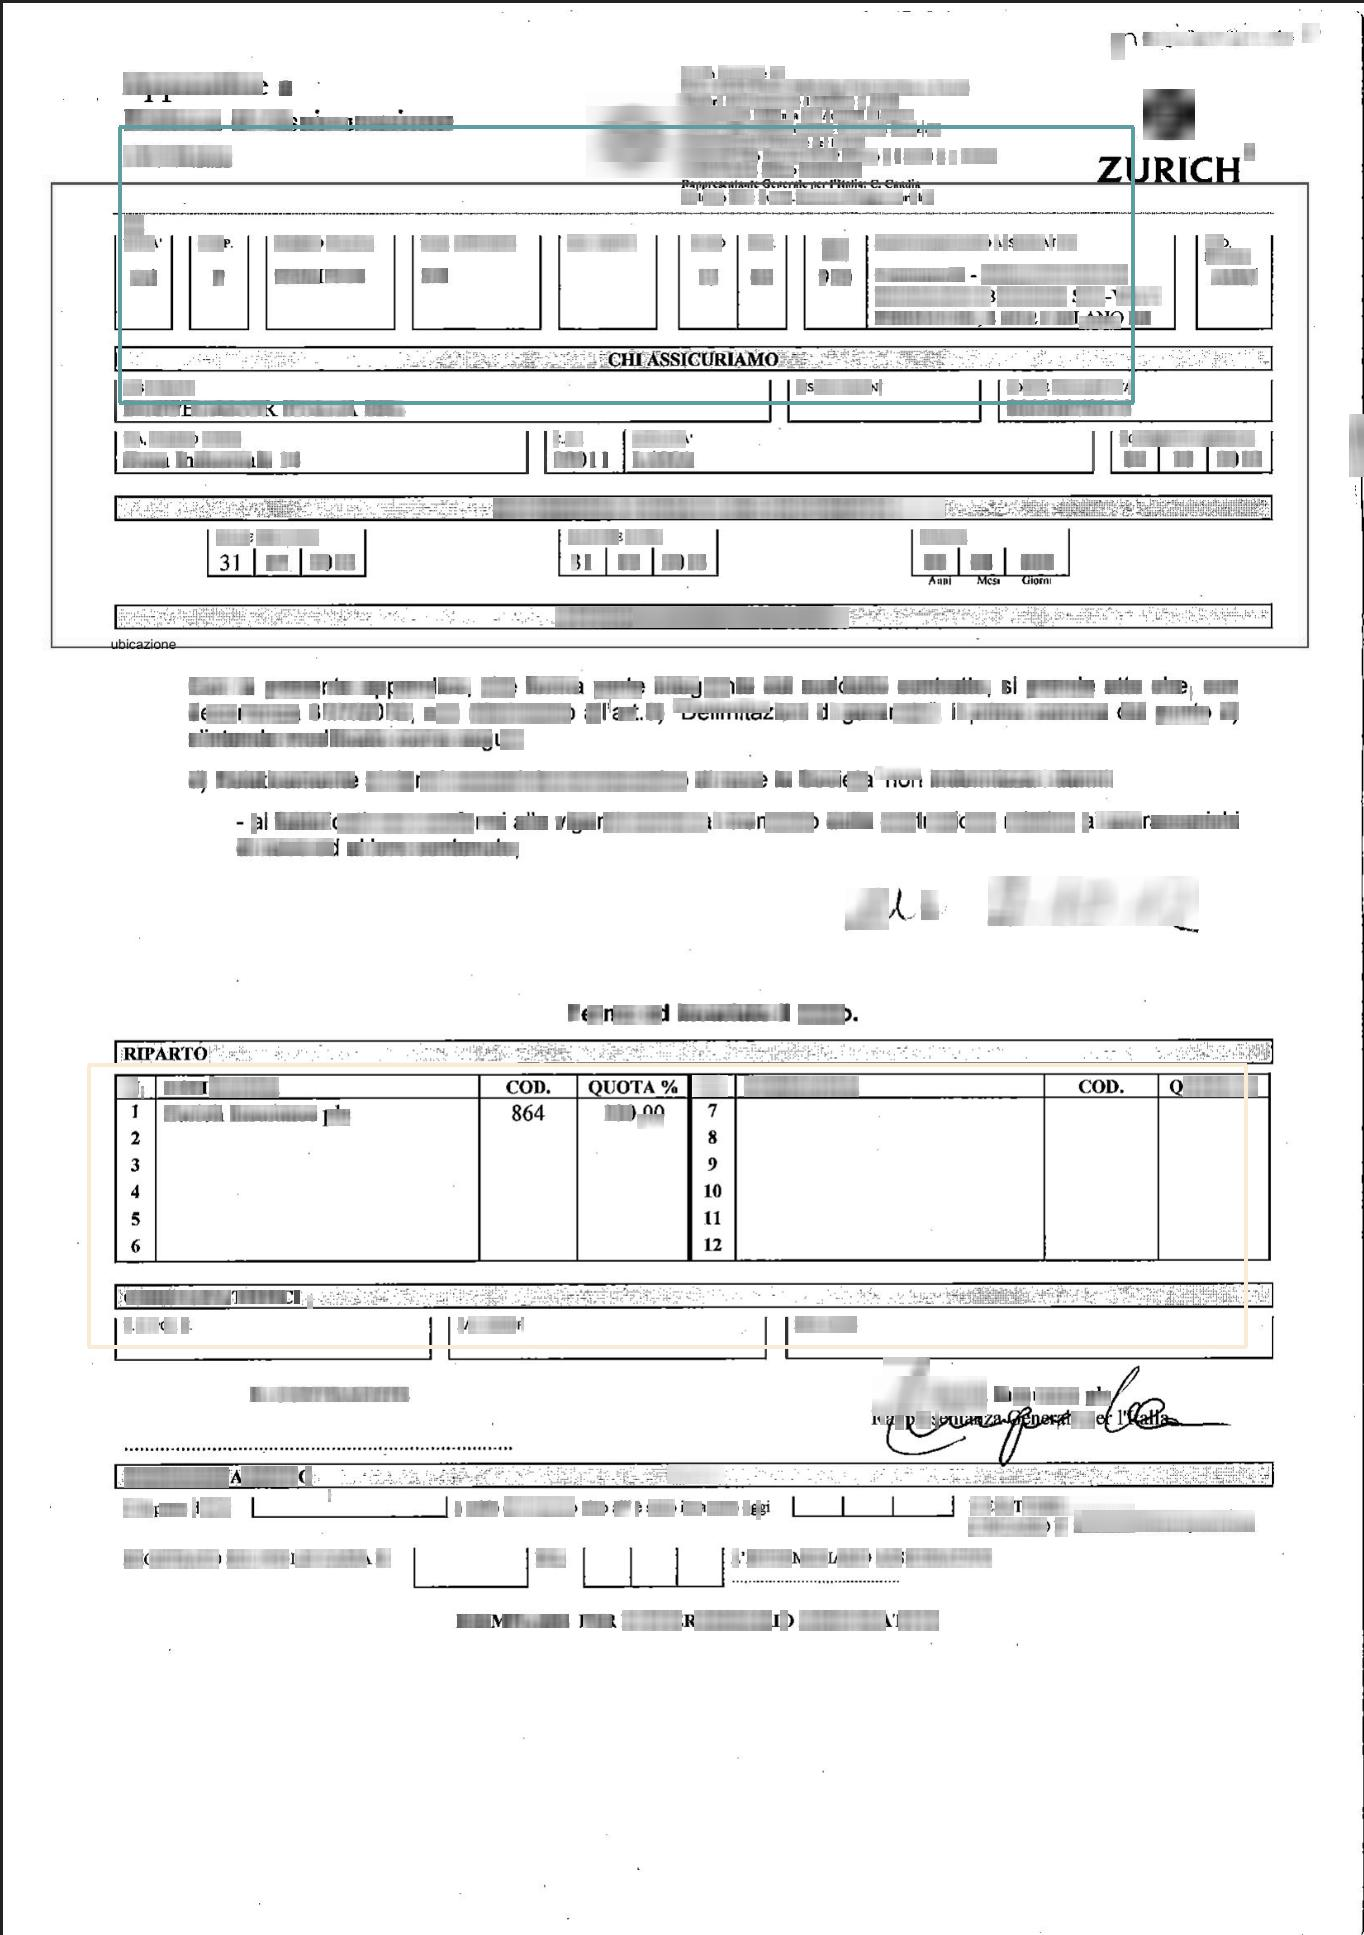
\includegraphics[width=1\columnwidth]{appendice/filtrate/test3_filtered_0_6_momentum_10k_jpg}  
    \end{minipage}%  
    \begin{minipage}{0.5\columnwidth}  
        \centering  
        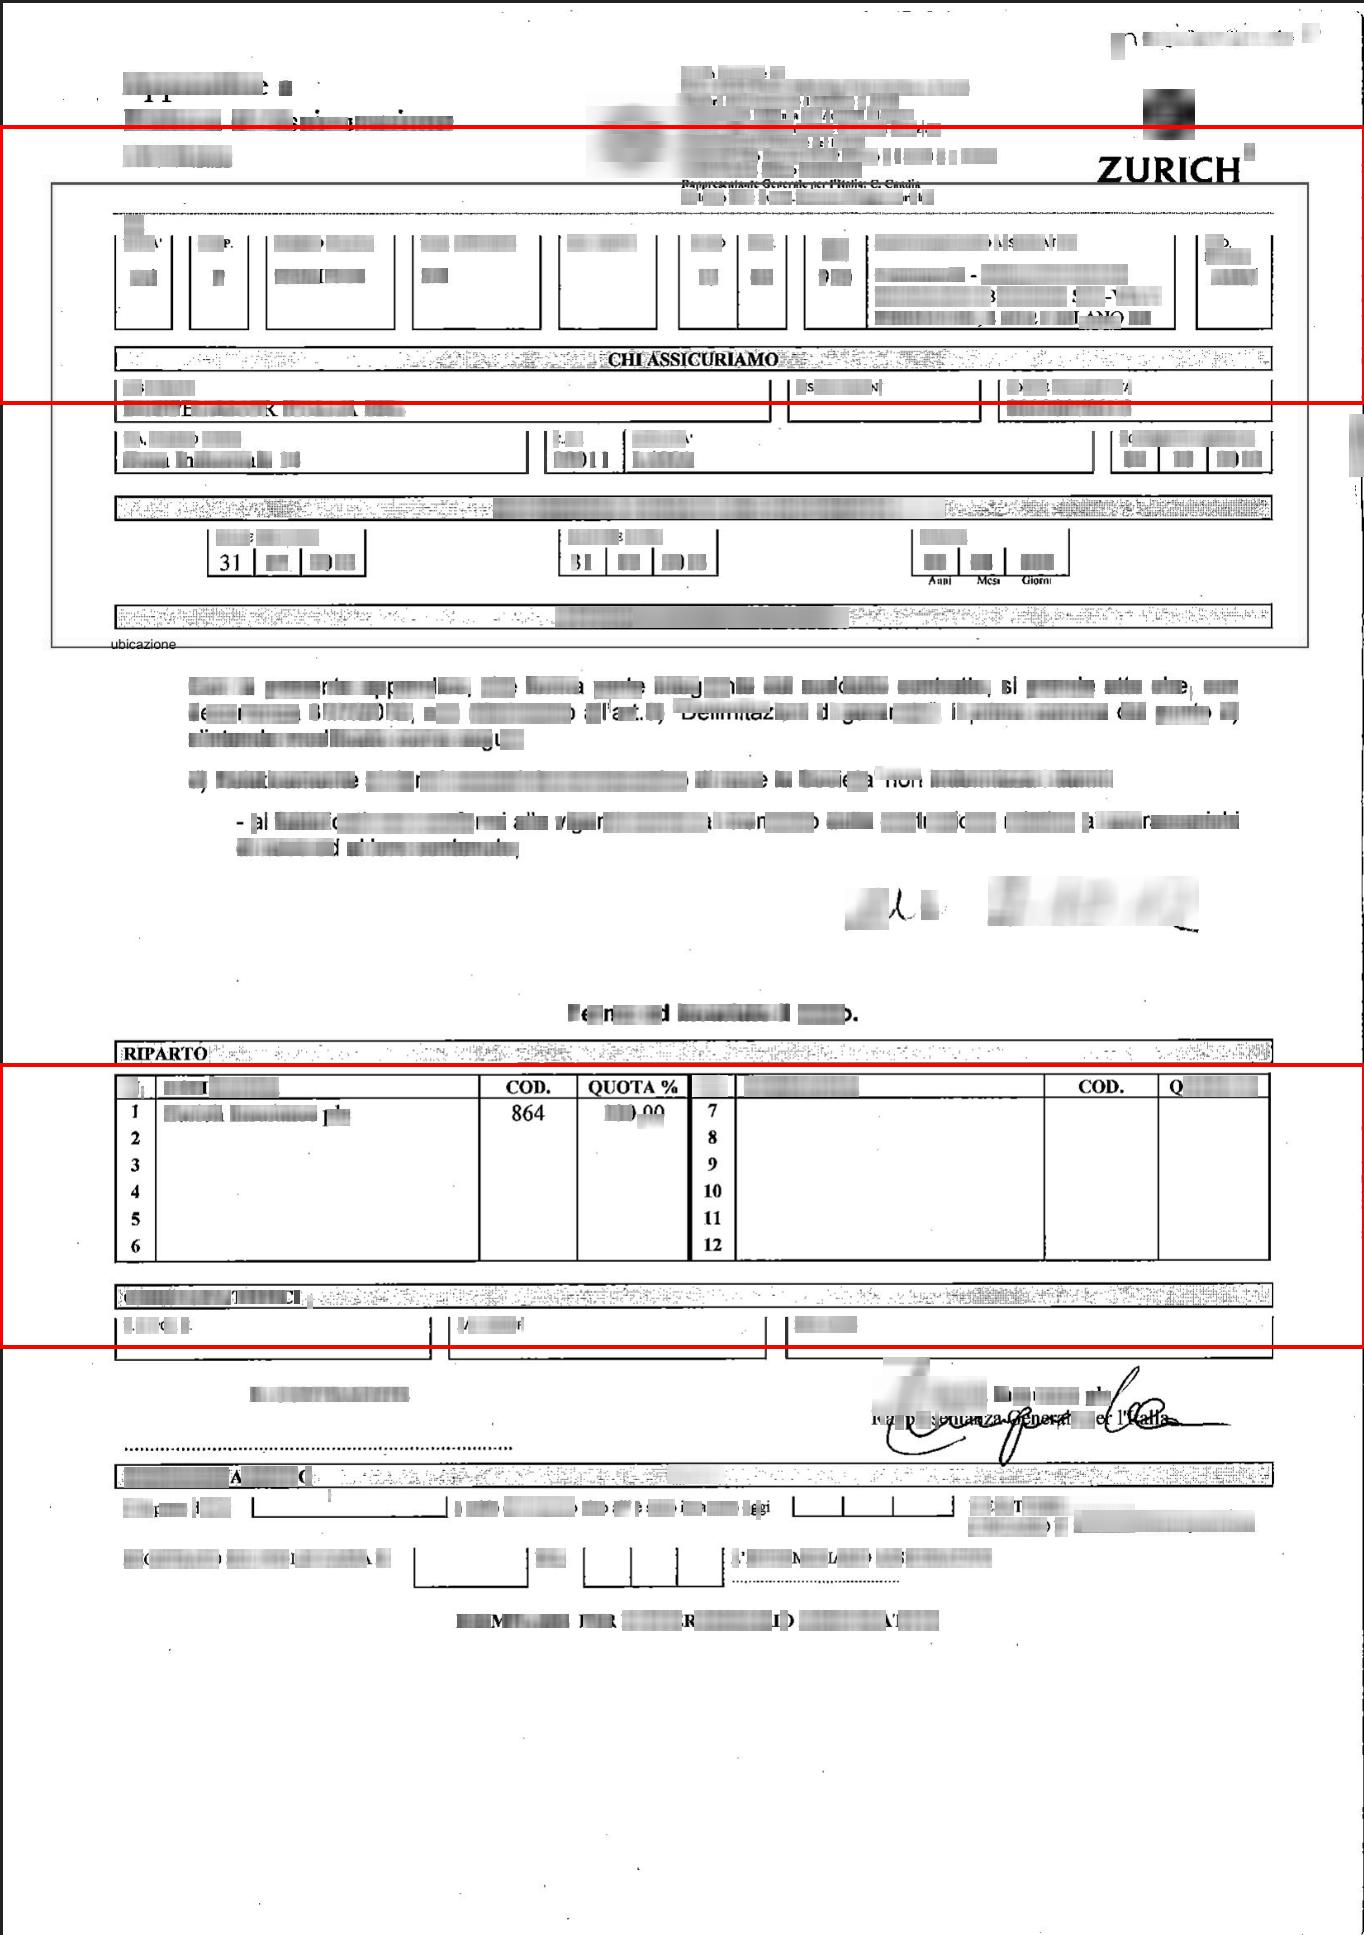
\includegraphics[width=1\columnwidth]{appendice/unite/test3_merged_0_6_momentum_10k_jpg}  
    \end{minipage}  
    \caption{Test 3, configurazione 5}
\end{figure}%  
Configurazione:
\begin{multicols}{2}
    \begin{lstlisting}
image_resizer {
  fixes_shape_resizer {
    width: 400
    heigth: 400
  }
}
first_stage_box_predictor {
  l2_regularizer {
    weight: 0.004
}
first_stage_nms_iou_threshold: 0.7
second_stage_box_predictor {
  l2_regularizer {
    weight: 0.004
  }
}
second_stage_post_processing {
  iou_threshold: 0.6
}
optimizer {
  adam_optimizer: {
    learning_rate: {
      manual_step_learning_rate {
        initial_learning_rate: 0.0004
        schedule {
          step: 4500
          learning_rate: .0002
        }
        schedule {
          step: 7000
          learning_rate: .00002
        }
        schedule {
          step: 10000
          learning_rate: .000002
        }
    ...
    }
    momentum_optimizer_value: 0.9
  }
  use_moving_average: false
}
    \end{lstlisting}
\end{multicols}
%============================================================================================

\newpage
\begin{figure}[H]  
    \begin{minipage}{.5\columnwidth}  
        \centering  
        \includegraphics[width=1\columnwidth]{appendice/filtrate/test3_filtered_0_6_momentum_optimizer_1batch}  
    \end{minipage}%  
    \begin{minipage}{0.5\columnwidth}  
        \centering  
        \includegraphics[width=1\columnwidth]{appendice/unite/test3_merged_0_6_momentum_optimizer_1batch}  
    \end{minipage}  
    \caption{Test 3, configurazione 6}
\end{figure}%  
Configurazione:
\begin{multicols}{2}
    \begin{lstlisting}
image_resizer {
  fixes_shape_resizer {
    width: 400
    heigth: 400
  }
}
first_stage_box_predictor {
  l2_regularizer {
    weight: 0.04
}
first_stage_nms_iou_threshold: 0.7
second_stage_box_predictor {
  l2_regularizer {
    weight: 0.004
  }
}
second_stage_post_processing {
  iou_threshold: 0.6
}
batch_size: 1
optimizer {
  adam_optimizer: {
    learning_rate: {
      manual_step_learning_rate {
        initial_learning_rate: 0.0004
        schedule {
          step: 4500
          learning_rate: .0002
        }
        schedule {
          step: 7000
          learning_rate: .00002
        }
        schedule {
          step: 10000
          learning_rate: .000002
        }
    ...
    }
    momentum_optimizer_value: 0.9
  }
  use_moving_average: false
}
    \end{lstlisting}
\end{multicols}
%============================================================================================
\newpage
\subsection{Test 4}
\begin{figure}[!ht] 
    \centering
    \includegraphics[width=1\columnwidth]{appendice/test4} 
    \caption{Test 4}
    \label{img:test-1}
\end{figure} 
\newpage

%============================================================================================


\begin{figure}[H]  
    \begin{minipage}{.5\columnwidth}  
        \centering  
        \includegraphics[width=1\columnwidth]{appendice/filtrate/test4_filtered_0_6_adam_1}  
    \end{minipage}%  
    \begin{minipage}{0.5\columnwidth}  
        \centering  
        \includegraphics[width=1\columnwidth]{appendice/unite/test4_merged_0_6_adam_1}  
    \end{minipage}  
    \caption{Test 4, configurazione 1}
\end{figure}%  
Configurazione:
\begin{multicols}{2}
    \begin{lstlisting}
image_resizer {
  fixes_shape_resizer {
    width: 400
    heigth: 400
  }
}
first_stage_box_predictor {
  l2_regularizer {
    weight: 0.008
}
first_stage_nms_iou_threshold: 0.7
second_stage_box_predictor {
  l2_regularizer {
    weight: 0.004
  }
}
second_stage_post_processing {
  iou_threshold: 0.6
}
optimizer {
  adam_optimizer: {
    learning_rate: {
      manual_step_learning_rate {
        initial_learning_rate: .00008
        schedule {
          step: 4500
          learning_rate: .00004
        }
        schedule {
          step: 7000
          learning_rate: .00002
        }
        schedule {
          step: 10000
          learning_rate: .000008
        }
    ...
    }
    momentum_optimizer_value: 0.9
  }
  use_moving_average: false
}
\end{lstlisting}
\end{multicols}

%============================================================================================
\newpage
\begin{figure}[H]  
    \begin{minipage}{.5\columnwidth}  
        \centering  
        \includegraphics[width=1\columnwidth]{appendice/filtrate/test4_filtered_0_6_adam_3}  
    \end{minipage}%  
    \begin{minipage}{0.5\columnwidth}  
        \centering  
        \includegraphics[width=1\columnwidth]{appendice/unite/test4_merged_0_6_adam_3}  
    \end{minipage}  
    \caption{Test 4, configurazione 2}
\end{figure}%  
Configurazione:
\begin{multicols}{2}
    \begin{lstlisting}
image_resizer {
  fixes_shape_resizer {
    width: 400
    heigth: 400
  }
}
first_stage_box_predictor {
  l2_regularizer {
    weight: 0.00001
}
first_stage_nms_iou_threshold: 0.7
second_stage_box_predictor {
  l2_regularizer {
    weight: 0.00004
  }
}
second_stage_post_processing {
  iou_threshold: 0.6
}
optimizer {
  adam_optimizer: {
    learning_rate: {
      exponential_decay_learning_rate {
        initial_learning_rate: 0.0001
          decay_steps: 600
          decay_factor: 0.95
        }
      }
    ...
  use_moving_average: false
}
    \end{lstlisting}
\end{multicols}

%============================================================================================
\newpage
\begin{figure}[H]  
    \begin{minipage}{.5\columnwidth}  
        \centering  
        \includegraphics[width=1\columnwidth]{appendice/filtrate/test4_filtered_0_6_adam_4}  
    \end{minipage}%  
    \begin{minipage}{0.5\columnwidth}  
        \centering  
        \includegraphics[width=1\columnwidth]{appendice/unite/test4_merged_0_6_adam_4}  
    \end{minipage}  
    \caption{Test 4, configurazione 3}
\end{figure}%  
Configurazione:
\begin{multicols}{2}
    \begin{lstlisting}
image_resizer {
  fixes_shape_resizer {
    width: 400
    heigth: 400
  }
}
first_stage_box_predictor {
  l2_regularizer {
    weight: 0.04
}
first_stage_nms_iou_threshold: 0.7
second_stage_box_predictor {
  l2_regularizer {
    weight: 0.004
  }
}
second_stage_post_processing {
  iou_threshold: 0.6
}
optimizer {
  adam_optimizer: {
    learning_rate: {
      exponential_decay_learning_rate {
        initial_learning_rate: 0.0001
          decay_steps: 450
          decay_factor: 0.9
        }
      }
    ...
  use_moving_average: false
}
    \end{lstlisting}
\end{multicols}

%============================================================================================
\newpage
\begin{figure}[H]  
    \begin{minipage}{.5\columnwidth}  
        \centering  
        \includegraphics[width=1\columnwidth]{appendice/filtrate/test4_filtered_0_6_momentum_1}  
    \end{minipage}%  
    \begin{minipage}{0.5\columnwidth}  
        \centering  
        \includegraphics[width=1\columnwidth]{appendice/unite/test4_merged_0_6_momentum_1}  
    \end{minipage}  
    \caption{Test 4, configurazione 4}
\end{figure}%  
Configurazione:
\begin{multicols}{2}
    \begin{lstlisting}
image_resizer {
  fixes_shape_resizer {
    width: 400
    heigth: 400
  }
}
first_stage_box_predictor {
  l2_regularizer {
    weight: 0.00001
}
first_stage_nms_iou_threshold: 0.7
second_stage_box_predictor {
  l2_regularizer {
    weight: 0.00004
  }
}
second_stage_post_processing {
  iou_threshold: 0.6
}
optimizer {
  adam_optimizer: {
    learning_rate: {
      manual_step_learning_rate {
        initial_learning_rate: 0.0008
        schedule {
          step: 4500
          learning_rate: .0008
        }
        schedule {
          step: 7000
          learning_rate: .0004
        }
        schedule {
          step: 10000
          learning_rate: .00008
        }
    ...
    }
    momentum_optimizer_value: 0.9
  }
  use_moving_average: false
}
    \end{lstlisting}
\end{multicols}
%============================================================================================

\newpage
\begin{figure}[H]  
    \begin{minipage}{.5\columnwidth}  
        \centering  
        \includegraphics[width=1\columnwidth]{appendice/filtrate/test4_filtered_0_6_momentum_10k_jpg}  
    \end{minipage}%  
    \begin{minipage}{0.5\columnwidth}  
        \centering  
        \includegraphics[width=1\columnwidth]{appendice/unite/test4_merged_0_6_momentum_10k_jpg}  
    \end{minipage}  
    \caption{Test 4, configurazione 5}
\end{figure}%  
Configurazione:
\begin{multicols}{2}
    \begin{lstlisting}
image_resizer {
  fixes_shape_resizer {
    width: 400
    heigth: 400
  }
}
first_stage_box_predictor {
  l2_regularizer {
    weight: 0.004
}
first_stage_nms_iou_threshold: 0.7
second_stage_box_predictor {
  l2_regularizer {
    weight: 0.004
  }
}
second_stage_post_processing {
  iou_threshold: 0.6
}
optimizer {
  adam_optimizer: {
    learning_rate: {
      manual_step_learning_rate {
        initial_learning_rate: 0.0004
        schedule {
          step: 4500
          learning_rate: .0002
        }
        schedule {
          step: 7000
          learning_rate: .00002
        }
        schedule {
          step: 10000
          learning_rate: .000002
        }
    ...
    }
    momentum_optimizer_value: 0.9
  }
  use_moving_average: false
}
    \end{lstlisting}
\end{multicols}
%============================================================================================

\newpage
\begin{figure}[H]  
    \begin{minipage}{.5\columnwidth}  
        \centering  
        \includegraphics[width=1\columnwidth]{appendice/filtrate/test4_filtered_0_6_momentum_optimizer_1batch}  
    \end{minipage}%  
    \begin{minipage}{0.5\columnwidth}  
        \centering  
        \includegraphics[width=1\columnwidth]{appendice/unite/test4_merged_0_6_momentum_optimizer_1batch}  
    \end{minipage}  
    \caption{Test 4, configurazione 6}
\end{figure}%  
Configurazione:
\begin{multicols}{2}
    \begin{lstlisting}
image_resizer {
  fixes_shape_resizer {
    width: 400
    heigth: 400
  }
}
first_stage_box_predictor {
  l2_regularizer {
    weight: 0.04
}
first_stage_nms_iou_threshold: 0.7
second_stage_box_predictor {
  l2_regularizer {
    weight: 0.004
  }
}
second_stage_post_processing {
  iou_threshold: 0.6
}
batch_size: 1
optimizer {
  adam_optimizer: {
    learning_rate: {
      manual_step_learning_rate {
        initial_learning_rate: 0.0004
        schedule {
          step: 4500
          learning_rate: .0002
        }
        schedule {
          step: 7000
          learning_rate: .00002
        }
        schedule {
          step: 10000
          learning_rate: .000002
        }
    ...
    }
    momentum_optimizer_value: 0.9
  }
  use_moving_average: false
}
    \end{lstlisting}
\end{multicols}
%============================================================================================
\newpage
\subsection{Test 5}
\begin{figure}[!ht] 
    \centering
    \includegraphics[width=1\columnwidth]{appendice/test5} 
    \caption{Test 5}
    \label{img:test-1}
\end{figure} 
\newpage

%============================================================================================


\begin{figure}[H]  
    \begin{minipage}{.5\columnwidth}  
        \centering  
        \includegraphics[width=1\columnwidth]{appendice/filtrate/test5_filtered_0_6_adam_1}  
    \end{minipage}%  
    \begin{minipage}{0.5\columnwidth}  
        \centering  
        \includegraphics[width=1\columnwidth]{appendice/unite/test5_merged_0_6_adam_1}  
    \end{minipage}  
    \caption{Test 5, configurazione 1}
\end{figure}%  
Configurazione:
\begin{multicols}{2}
    \begin{lstlisting}
image_resizer {
  fixes_shape_resizer {
    width: 400
    heigth: 400
  }
}
first_stage_box_predictor {
  l2_regularizer {
    weight: 0.008
}
first_stage_nms_iou_threshold: 0.7
second_stage_box_predictor {
  l2_regularizer {
    weight: 0.004
  }
}
second_stage_post_processing {
  iou_threshold: 0.6
}
optimizer {
  adam_optimizer: {
    learning_rate: {
      manual_step_learning_rate {
        initial_learning_rate: .00008
        schedule {
          step: 4500
          learning_rate: .00004
        }
        schedule {
          step: 7000
          learning_rate: .00002
        }
        schedule {
          step: 10000
          learning_rate: .000008
        }
    ...
    }
    momentum_optimizer_value: 0.9
  }
  use_moving_average: false
}
\end{lstlisting}
\end{multicols}

%============================================================================================
\newpage
\begin{figure}[H]  
    \begin{minipage}{.5\columnwidth}  
        \centering  
        \includegraphics[width=1\columnwidth]{appendice/filtrate/test5_filtered_0_6_adam_3}  
    \end{minipage}%  
    \begin{minipage}{0.5\columnwidth}  
        \centering  
        \includegraphics[width=1\columnwidth]{appendice/unite/test5_merged_0_6_adam_3}  
    \end{minipage}  
    \caption{Test 5, configurazione 2}
\end{figure}%  
Configurazione:
\begin{multicols}{2}
    \begin{lstlisting}
image_resizer {
  fixes_shape_resizer {
    width: 400
    heigth: 400
  }
}
first_stage_box_predictor {
  l2_regularizer {
    weight: 0.00001
}
first_stage_nms_iou_threshold: 0.7
second_stage_box_predictor {
  l2_regularizer {
    weight: 0.00004
  }
}
second_stage_post_processing {
  iou_threshold: 0.6
}
optimizer {
  adam_optimizer: {
    learning_rate: {
      exponential_decay_learning_rate {
        initial_learning_rate: 0.0001
          decay_steps: 600
          decay_factor: 0.95
        }
      }
    ...
  use_moving_average: false
}
    \end{lstlisting}
\end{multicols}

%============================================================================================
\newpage
\begin{figure}[H]  
    \begin{minipage}{.5\columnwidth}  
        \centering  
        \includegraphics[width=1\columnwidth]{appendice/filtrate/test5_filtered_0_6_adam_4}  
    \end{minipage}%  
    \begin{minipage}{0.5\columnwidth}  
        \centering  
        \includegraphics[width=1\columnwidth]{appendice/unite/test5_merged_0_6_adam_4}  
    \end{minipage}  
    \caption{Test 5, configurazione 3}
\end{figure}%  
Configurazione:
\begin{multicols}{2}
    \begin{lstlisting}
image_resizer {
  fixes_shape_resizer {
    width: 400
    heigth: 400
  }
}
first_stage_box_predictor {
  l2_regularizer {
    weight: 0.04
}
first_stage_nms_iou_threshold: 0.7
second_stage_box_predictor {
  l2_regularizer {
    weight: 0.004
  }
}
second_stage_post_processing {
  iou_threshold: 0.6
}
optimizer {
  adam_optimizer: {
    learning_rate: {
      exponential_decay_learning_rate {
        initial_learning_rate: 0.0001
          decay_steps: 450
          decay_factor: 0.9
        }
      }
    ...
  use_moving_average: false
}
    \end{lstlisting}
\end{multicols}

%============================================================================================
\newpage
\begin{figure}[H]  
    \begin{minipage}{.5\columnwidth}  
        \centering  
        \includegraphics[width=1\columnwidth]{appendice/filtrate/test5_filtered_0_6_momentum_1}  
    \end{minipage}%  
    \begin{minipage}{0.5\columnwidth}  
        \centering  
        \includegraphics[width=1\columnwidth]{appendice/unite/test5_merged_0_6_momentum_1}  
    \end{minipage}  
    \caption{Test 5, configurazione 4}
\end{figure}%  
Configurazione:
\begin{multicols}{2}
    \begin{lstlisting}
image_resizer {
  fixes_shape_resizer {
    width: 400
    heigth: 400
  }
}
first_stage_box_predictor {
  l2_regularizer {
    weight: 0.00001
}
first_stage_nms_iou_threshold: 0.7
second_stage_box_predictor {
  l2_regularizer {
    weight: 0.00004
  }
}
second_stage_post_processing {
  iou_threshold: 0.6
}
optimizer {
  adam_optimizer: {
    learning_rate: {
      manual_step_learning_rate {
        initial_learning_rate: 0.0008
        schedule {
          step: 4500
          learning_rate: .0008
        }
        schedule {
          step: 7000
          learning_rate: .0004
        }
        schedule {
          step: 10000
          learning_rate: .00008
        }
    ...
    }
    momentum_optimizer_value: 0.9
  }
  use_moving_average: false
}
    \end{lstlisting}
\end{multicols}
%============================================================================================

\newpage
\begin{figure}[H]  
    \begin{minipage}{.5\columnwidth}  
        \centering  
        \includegraphics[width=1\columnwidth]{appendice/filtrate/test5_filtered_0_6_momentum_10k_jpg}  
    \end{minipage}%  
    \begin{minipage}{0.5\columnwidth}  
        \centering  
        \includegraphics[width=1\columnwidth]{appendice/unite/test5_merged_0_6_momentum_10k_jpg}  
    \end{minipage}  
    \caption{Test 5, configurazione 5}
\end{figure}%  
Configurazione:
\begin{multicols}{2}
    \begin{lstlisting}
image_resizer {
  fixes_shape_resizer {
    width: 400
    heigth: 400
  }
}
first_stage_box_predictor {
  l2_regularizer {
    weight: 0.004
}
first_stage_nms_iou_threshold: 0.7
second_stage_box_predictor {
  l2_regularizer {
    weight: 0.004
  }
}
second_stage_post_processing {
  iou_threshold: 0.6
}
optimizer {
  adam_optimizer: {
    learning_rate: {
      manual_step_learning_rate {
        initial_learning_rate: 0.0004
        schedule {
          step: 4500
          learning_rate: .0002
        }
        schedule {
          step: 7000
          learning_rate: .00002
        }
        schedule {
          step: 10000
          learning_rate: .000002
        }
    ...
    }
    momentum_optimizer_value: 0.9
  }
  use_moving_average: false
}
    \end{lstlisting}
\end{multicols}
%============================================================================================

\newpage
\begin{figure}[H]  
    \begin{minipage}{.5\columnwidth}  
        \centering  
        \includegraphics[width=1\columnwidth]{appendice/filtrate/test5_filtered_0_6_momentum_optimizer_1batch}  
    \end{minipage}%  
    \begin{minipage}{0.5\columnwidth}  
        \centering  
        \includegraphics[width=1\columnwidth]{appendice/unite/test5_merged_0_6_momentum_optimizer_1batch}  
    \end{minipage}  
    \caption{Test 5, configurazione 6}
\end{figure}%  
Configurazione:
\begin{multicols}{2}
    \begin{lstlisting}
image_resizer {
  fixes_shape_resizer {
    width: 400
    heigth: 400
  }
}
first_stage_box_predictor {
  l2_regularizer {
    weight: 0.04
}
first_stage_nms_iou_threshold: 0.7
second_stage_box_predictor {
  l2_regularizer {
    weight: 0.004
  }
}
second_stage_post_processing {
  iou_threshold: 0.6
}
batch_size: 1
optimizer {
  adam_optimizer: {
    learning_rate: {
      manual_step_learning_rate {
        initial_learning_rate: 0.0004
        schedule {
          step: 4500
          learning_rate: .0002
        }
        schedule {
          step: 7000
          learning_rate: .00002
        }
        schedule {
          step: 10000
          learning_rate: .000002
        }
    ...
    }
    momentum_optimizer_value: 0.9
  }
  use_moving_average: false
}
    \end{lstlisting}
\end{multicols}
%============================================================================================

\section{\textit{Crop} da polizze assicurative}
\label{sec:crop-polizze-assicurative}
In questa sezione vengono mostrati i risultati dell'esecuzione dell'algoritmo su polizze assicurative facenti parte del \textit{dataset} datomi in dotazione. Si potrà notare come in alcuni casi l'inferenza abbia avuto risultati sorprendenti, altri in cui si denotano errori grossolani.

\newpage
\subsection{Test 0}
\begin{figure}[H] 
    \centering
    \includegraphics[width=1\columnwidth]{appendice/risultati/test0_full} 
    \caption{Test 0, pagina intera}
    \label{img:test-0-full}
\end{figure} 
\newpage
\begin{figure}[H]  
        \centering  
        \includegraphics[width=0.9\columnwidth]{appendice/risultati/test0_table}  
        \caption{Test 0, tabelle rilevate}
\end{figure}
\begin{figure}[H]
        \centering  
        \includegraphics[width=0.9\columnwidth]{appendice/risultati/test0_text}  
        \caption{Test 0, testo rimanente}
\end{figure}%  
%=============================================================================
\newpage
\subsection{Test 1}
\begin{figure}[H] 
    \centering
    \includegraphics[width=1\columnwidth]{appendice/risultati/test1_full} 
    \caption{Test 1, pagina intera}
    \label{img:test-0-full}
\end{figure} 
\newpage
\begin{figure}[H]  
        \centering  
        \includegraphics[width=0.9\columnwidth]{appendice/risultati/test1_table}  
        \caption{Test 1, tabelle rilevate}
\end{figure}
\begin{figure}[H]
        \centering  
        \includegraphics[width=0.9\columnwidth]{appendice/risultati/test1_text}  
        \caption{Test 1, testo rimanente}
\end{figure}%  
%=============================================================================
\newpage
\subsection{Test 2}
\label{sec:bad-test}
\begin{figure}[H] 
    \centering
    \includegraphics[width=1\columnwidth]{appendice/risultati/test2_full} 
    \caption{Test 2, pagina intera}
    \label{img:test-0-full}
\end{figure} 
\newpage
\begin{figure}[H]  
        \centering  
        \includegraphics[width=0.9\columnwidth]{appendice/risultati/test2_table}  
        \caption{Test 2, tabelle rilevate}
\end{figure}
\begin{figure}[H]
        \centering  
        \includegraphics[width=0.9\columnwidth]{appendice/risultati/test2_text}  
        \caption{Test 2, testo rimanente}
\end{figure}%  
%=============================================================================
\newpage
\subsection{Test 3}
\label{sec:good-test}
\begin{figure}[H] 
    \centering
    \includegraphics[width=1\columnwidth]{appendice/risultati/test3_full} 
    \caption{Test 3, pagina intera}
    \label{img:test-0-full}
\end{figure} 
\newpage
\begin{figure}[H]  
        \centering  
        \includegraphics[width=0.9\columnwidth]{appendice/risultati/test3_table}  
        \caption{Test 3, tabelle rilevate}
\end{figure}
\begin{figure}[H]
        \centering  
        \includegraphics[width=0.9\columnwidth]{appendice/risultati/test3_text}  
        \caption{Test 3, testo rimanente}
\end{figure}%  
%=============================================================================
\newpage
\subsection{Test 4}
\begin{figure}[H] 
    \centering
    \includegraphics[width=1\columnwidth]{appendice/risultati/test4_full} 
    \caption{Test 4, pagina intera}
    \label{img:test-0-full}
\end{figure} 
\newpage
\begin{figure}[H]  
        \centering  
        \includegraphics[width=0.9\columnwidth]{appendice/risultati/test4_table}  
        \caption{Test 4, tabelle rilevate}
\end{figure}
\begin{figure}[H]
        \centering  
        \includegraphics[width=0.9\columnwidth]{appendice/risultati/test4_text}  
        \caption{Test 4, testo rimanente}
\end{figure}%  
%=============================================================================
\newpage
\subsection{Test 5}
\begin{figure}[H] 
    \centering
    \includegraphics[width=1\columnwidth]{appendice/risultati/test5_full} 
    \caption{Test 5, pagina intera}
    \label{img:test-0-full}
\end{figure} 
\newpage
\begin{figure}[H]  
        \centering  
        \includegraphics[width=0.9\columnwidth]{appendice/risultati/test5_table}  
        \caption{Test 5, tabelle rilevate}
\end{figure}
\begin{figure}[H]
        \centering  
        \includegraphics[width=0.9\columnwidth]{appendice/risultati/test5_text}  
        \caption{Test 5, testo rimanente}
\end{figure}%  
%=============================================================================
%\newpage
%\subsection{Test 0}
%\begin{figure}[H] 
%    \centering
%    \includegraphics[width=1\columnwidth]{appendice/risultati/Test0_full} 
%    \caption{Test 0, pagina intera}
%    \label{img:test-0-full}
%\end{figure} 
%\newpage
%\begin{figure}[H]  
%        \centering  
%        \includegraphics[width=1\columnwidth]{appendice/risultati/test0_table}  
%        \caption{Test 0, tabelle rilevate}
%\end{figure}
%\begin{figure}[H]
%        \centering  
%        \includegraphics[width=1\columnwidth]{appendice/risultati/test0_text}  
%        \caption{Test 0, testo rimanente}
%\end{figure}%  
%%=============================================================================

